\section{Getting Started}
\label{sec:getting-started}

\subsection{Installation}
\label{sec:installation}

\subsubsection{Setup}
\label{sec:setup}

\begin{itemize}
\item Before installing the CamilleX feature, you need to add the XText update site (\url{http://download.eclipse.org/modeling/tmf/xtext/updates/composite/releases/}) as an additional software site (see Figure~\ref{fig:xtext-updatesite}).
\begin{figure}[!htbp]
  \centering
  \ifdef{PLASTEX}
  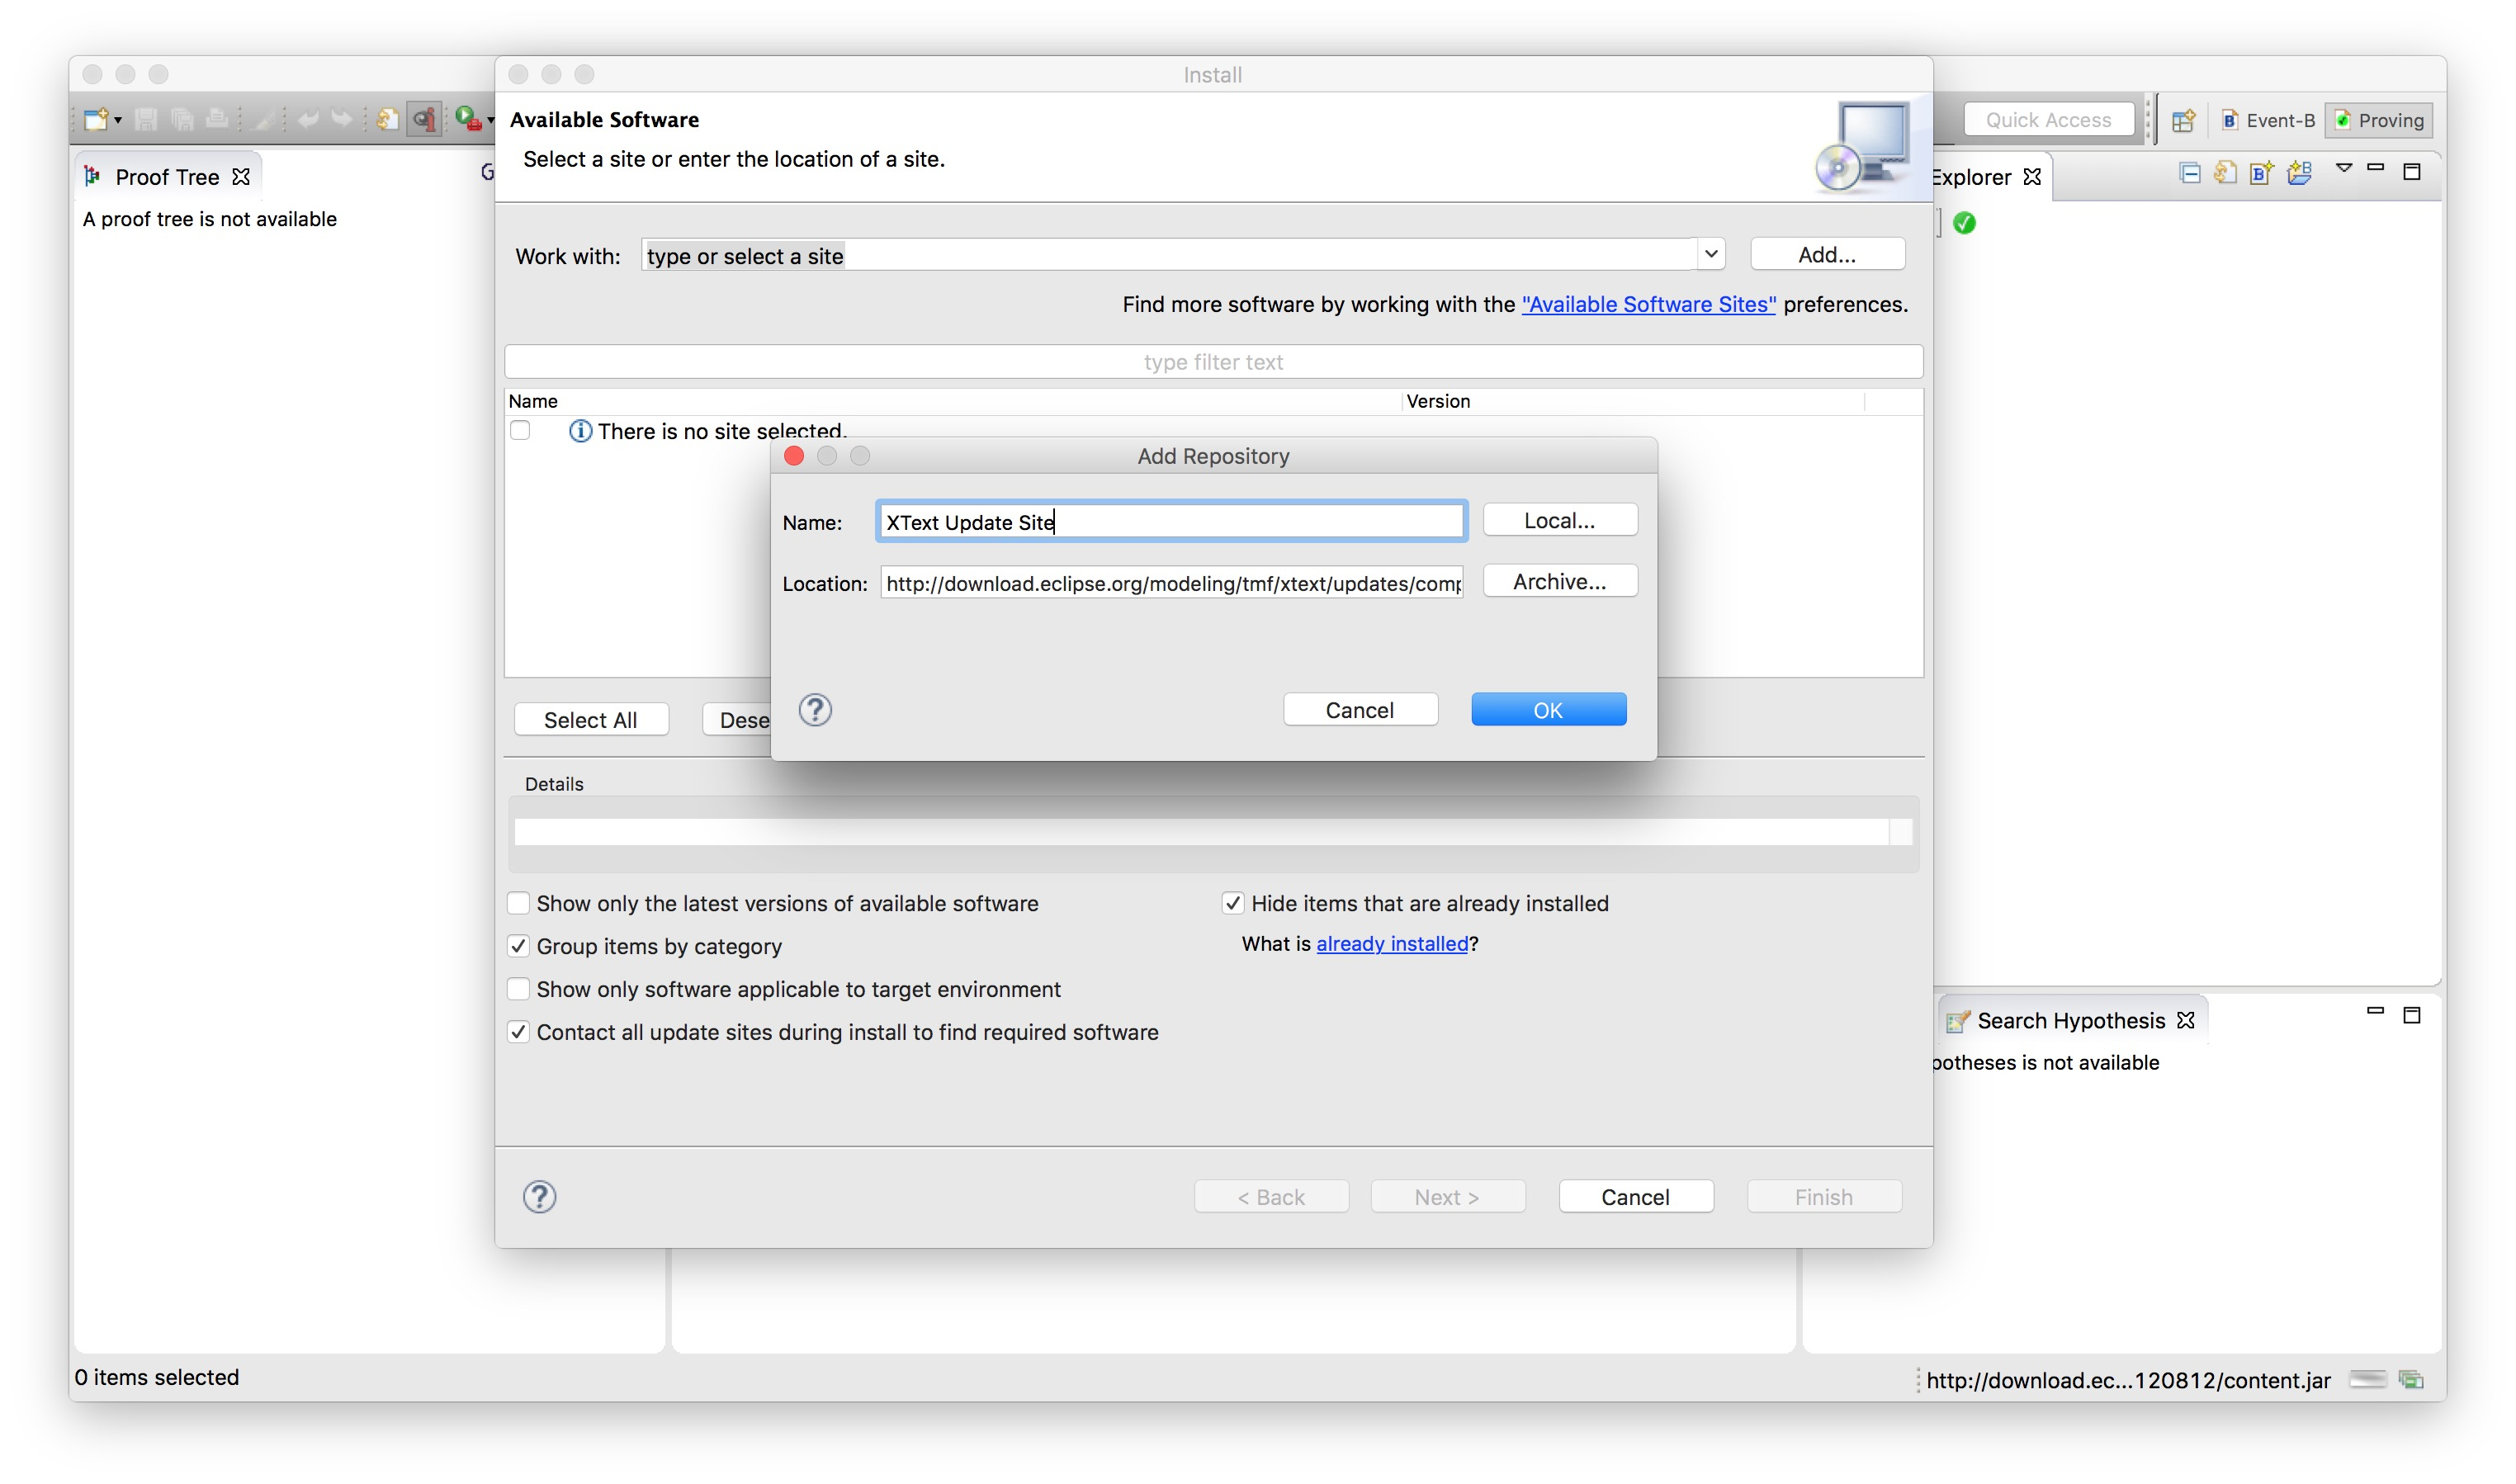
\includegraphics[width=512]{figures/XTextUpdateSite}
  \else
  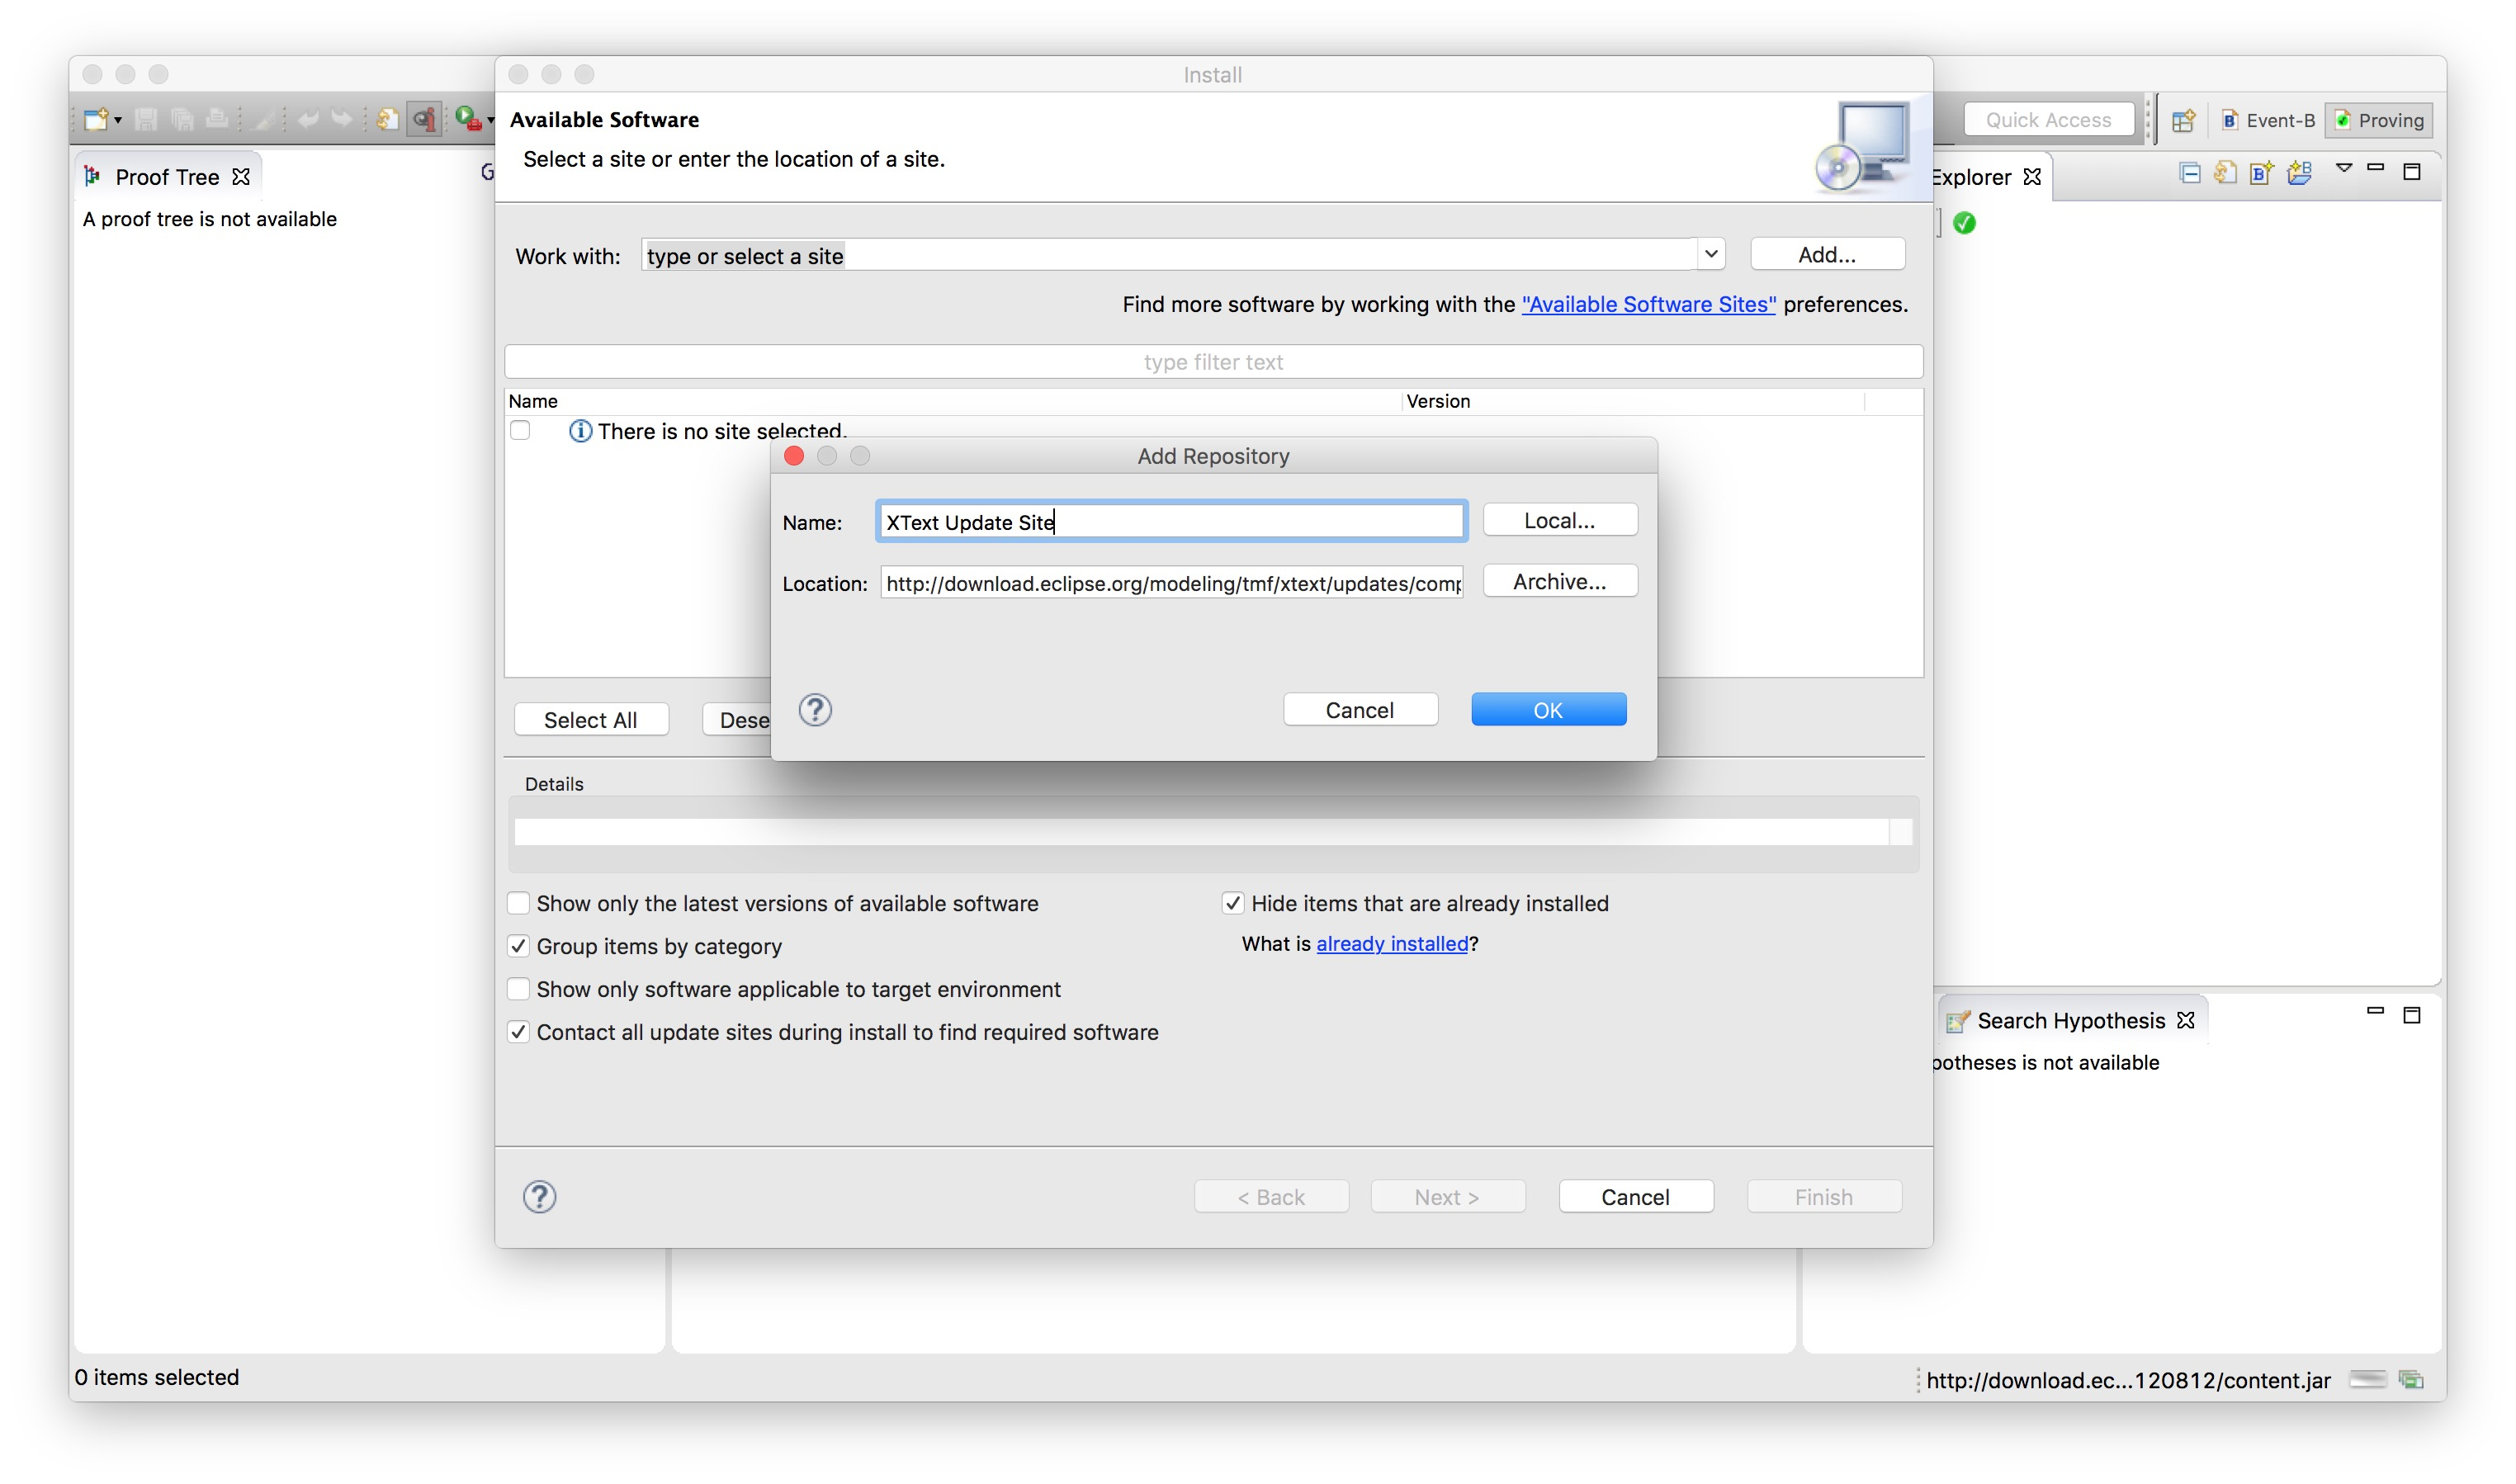
\includegraphics[width=0.9\textwidth]{figures/XTextUpdateSite}
  \endif
  \caption{Adding XText Update Site}
  \label{fig:xtext-updatesite}
\end{figure}


\item The CamilleX feature is available from the main Rodin update site (under ``Modelling Extensions'' category). There are two versions of the feature, \emph{CamilleX} providing facilities for working with CamilleX, and the \emph{CamilleX (SDK)} is the feature including source code for software developers (see Figure~\ref{fig:EventBXText-installation}).
\begin{figure}[!htbp]
  \centering
  \ifdef{PLASTEX}
  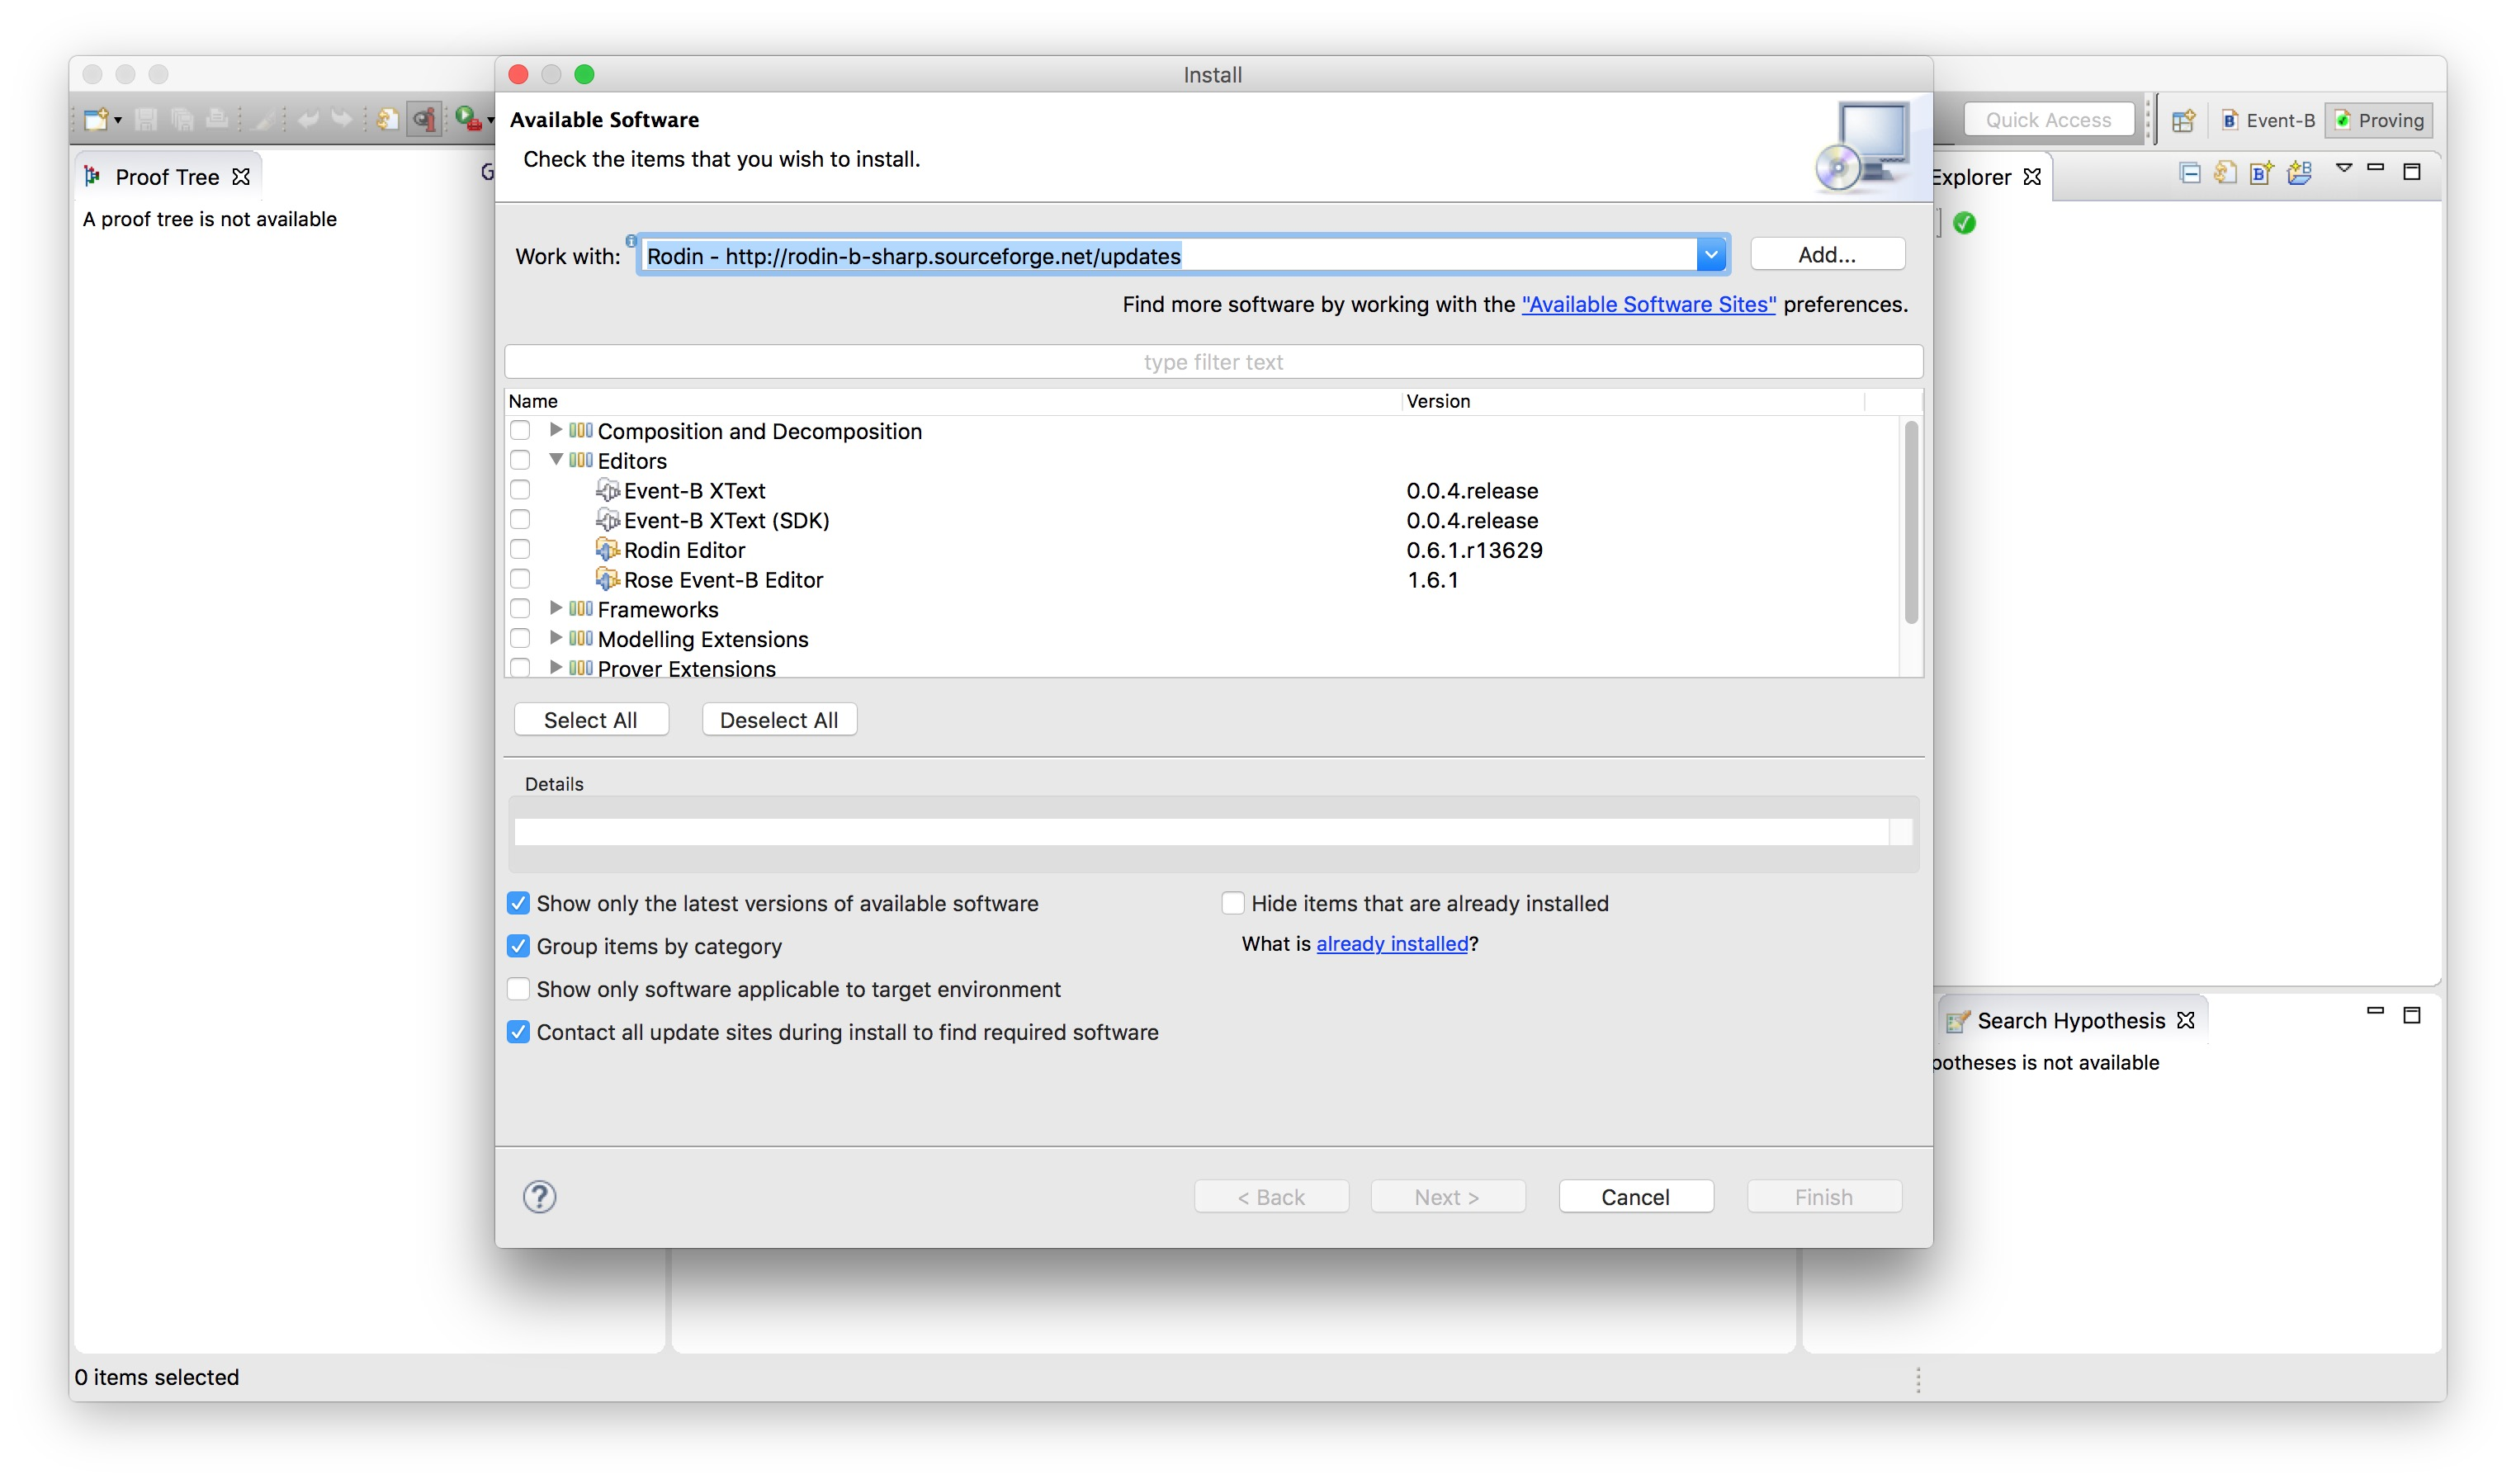
\includegraphics[width=512]{figures/EventBXTextInstallation}
  \else
  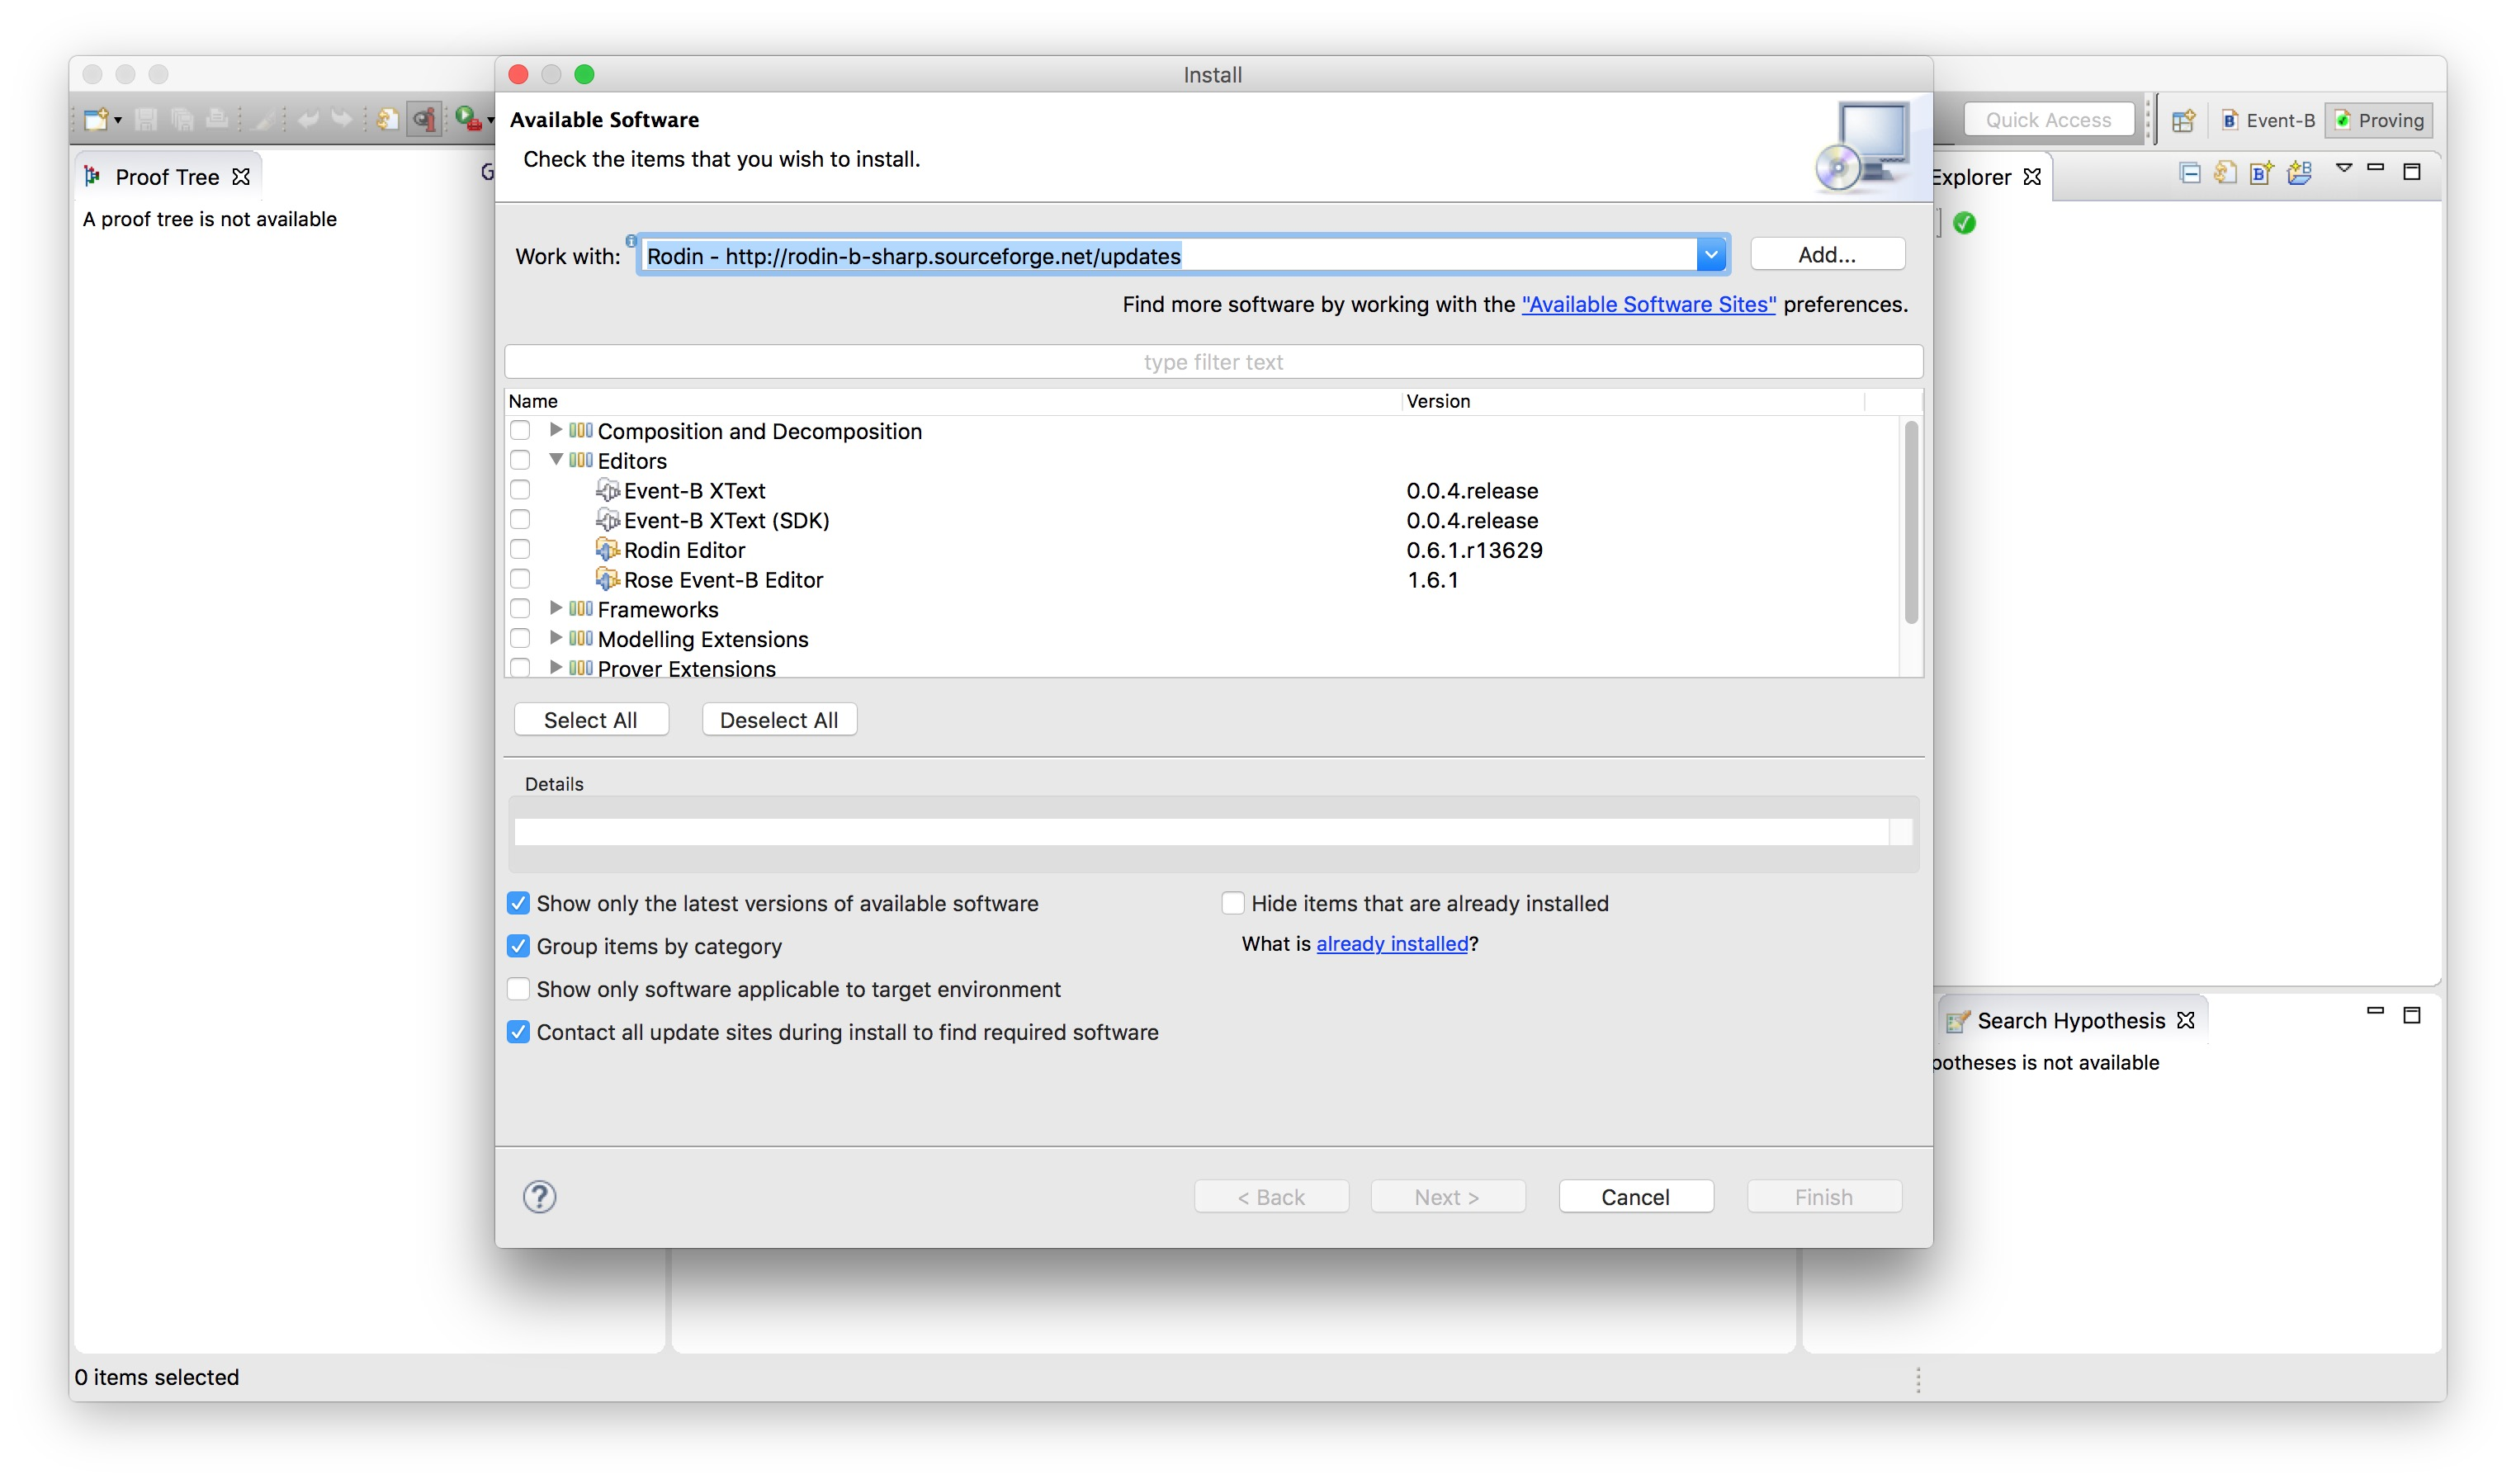
\includegraphics[width=0.9\textwidth]{figures/EventBXTextInstallation}
  \endif
  \caption{Adding XText Update Site}
  \label{fig:EventBXText-installation}
\end{figure}

\end{itemize}

\subsubsection{IMPORTANT}
\label{sec:important}

\begin{itemize}
\item Currently, CamilleX \textbf{not only} supports ``standard'' Event-B machines and contexts, but also supports ``\emph{Machine Inclusion}'' and ``\emph{Event Synchronisation}''.

\item Since the XContexts and XMachines are compiled to the Rodin files, the corresponding Rodin contexts and machines will be \textbf{OVER-WRITTEN}. Any changes in the Rodin files will not be lost.

\item \textbf{DO NOT USE} the CamilleX if you use modelling plug-ins such as \emph{iUML-B} state-machines and class-diagrams, as the additional modelling elements will be over-written.

\item Windows users \textbf{must} change the workspace text file encoding to \textbf{UTF-8}. This can be updated under the Rodin Preferences: General/Workspace then in the ``\emph{Text file encoding}'' section, select Other: UTF-8.

\end{itemize}

\subsubsection{Known Issues}
\label{sec:known-issues}

\begin{itemize}
\item Machine Inclusion: 
\begin{itemize}
	\item Including the \textbf{same} machine to both the abstract and its refining machine can result in the repetition of invariants.
\end{itemize}

\end{itemize}

\subsection{Basic Tutorial}
\label{sec:basic-tutorial}

This tutorial provides a step-by-step walk-through working with CamilleX constructs. This tutorial also available as Cheatsheets with the Rodin Platform (\texttt{Help/Cheat Sheets/CamilleX Cheatsheets/CamilleX Basic Tutorial}).

\subsubsection{Task 1. Create an Event-B Project}\label{CreateProject}
\textbf{Introduction} The purpose of this task is to create an Event-B project for the XEvent-B constructs. 
\begin{description}
\item[Step 1. Create a new Event-B Project] Create a new Event-B Project named ``Club'' using the \emph{New Event-B Project} wizard (see Figure~\ref{fig:CreateProject}).
\begin{figure}[!htbp]
  \centering
  \ifdef{PLASTEX}
  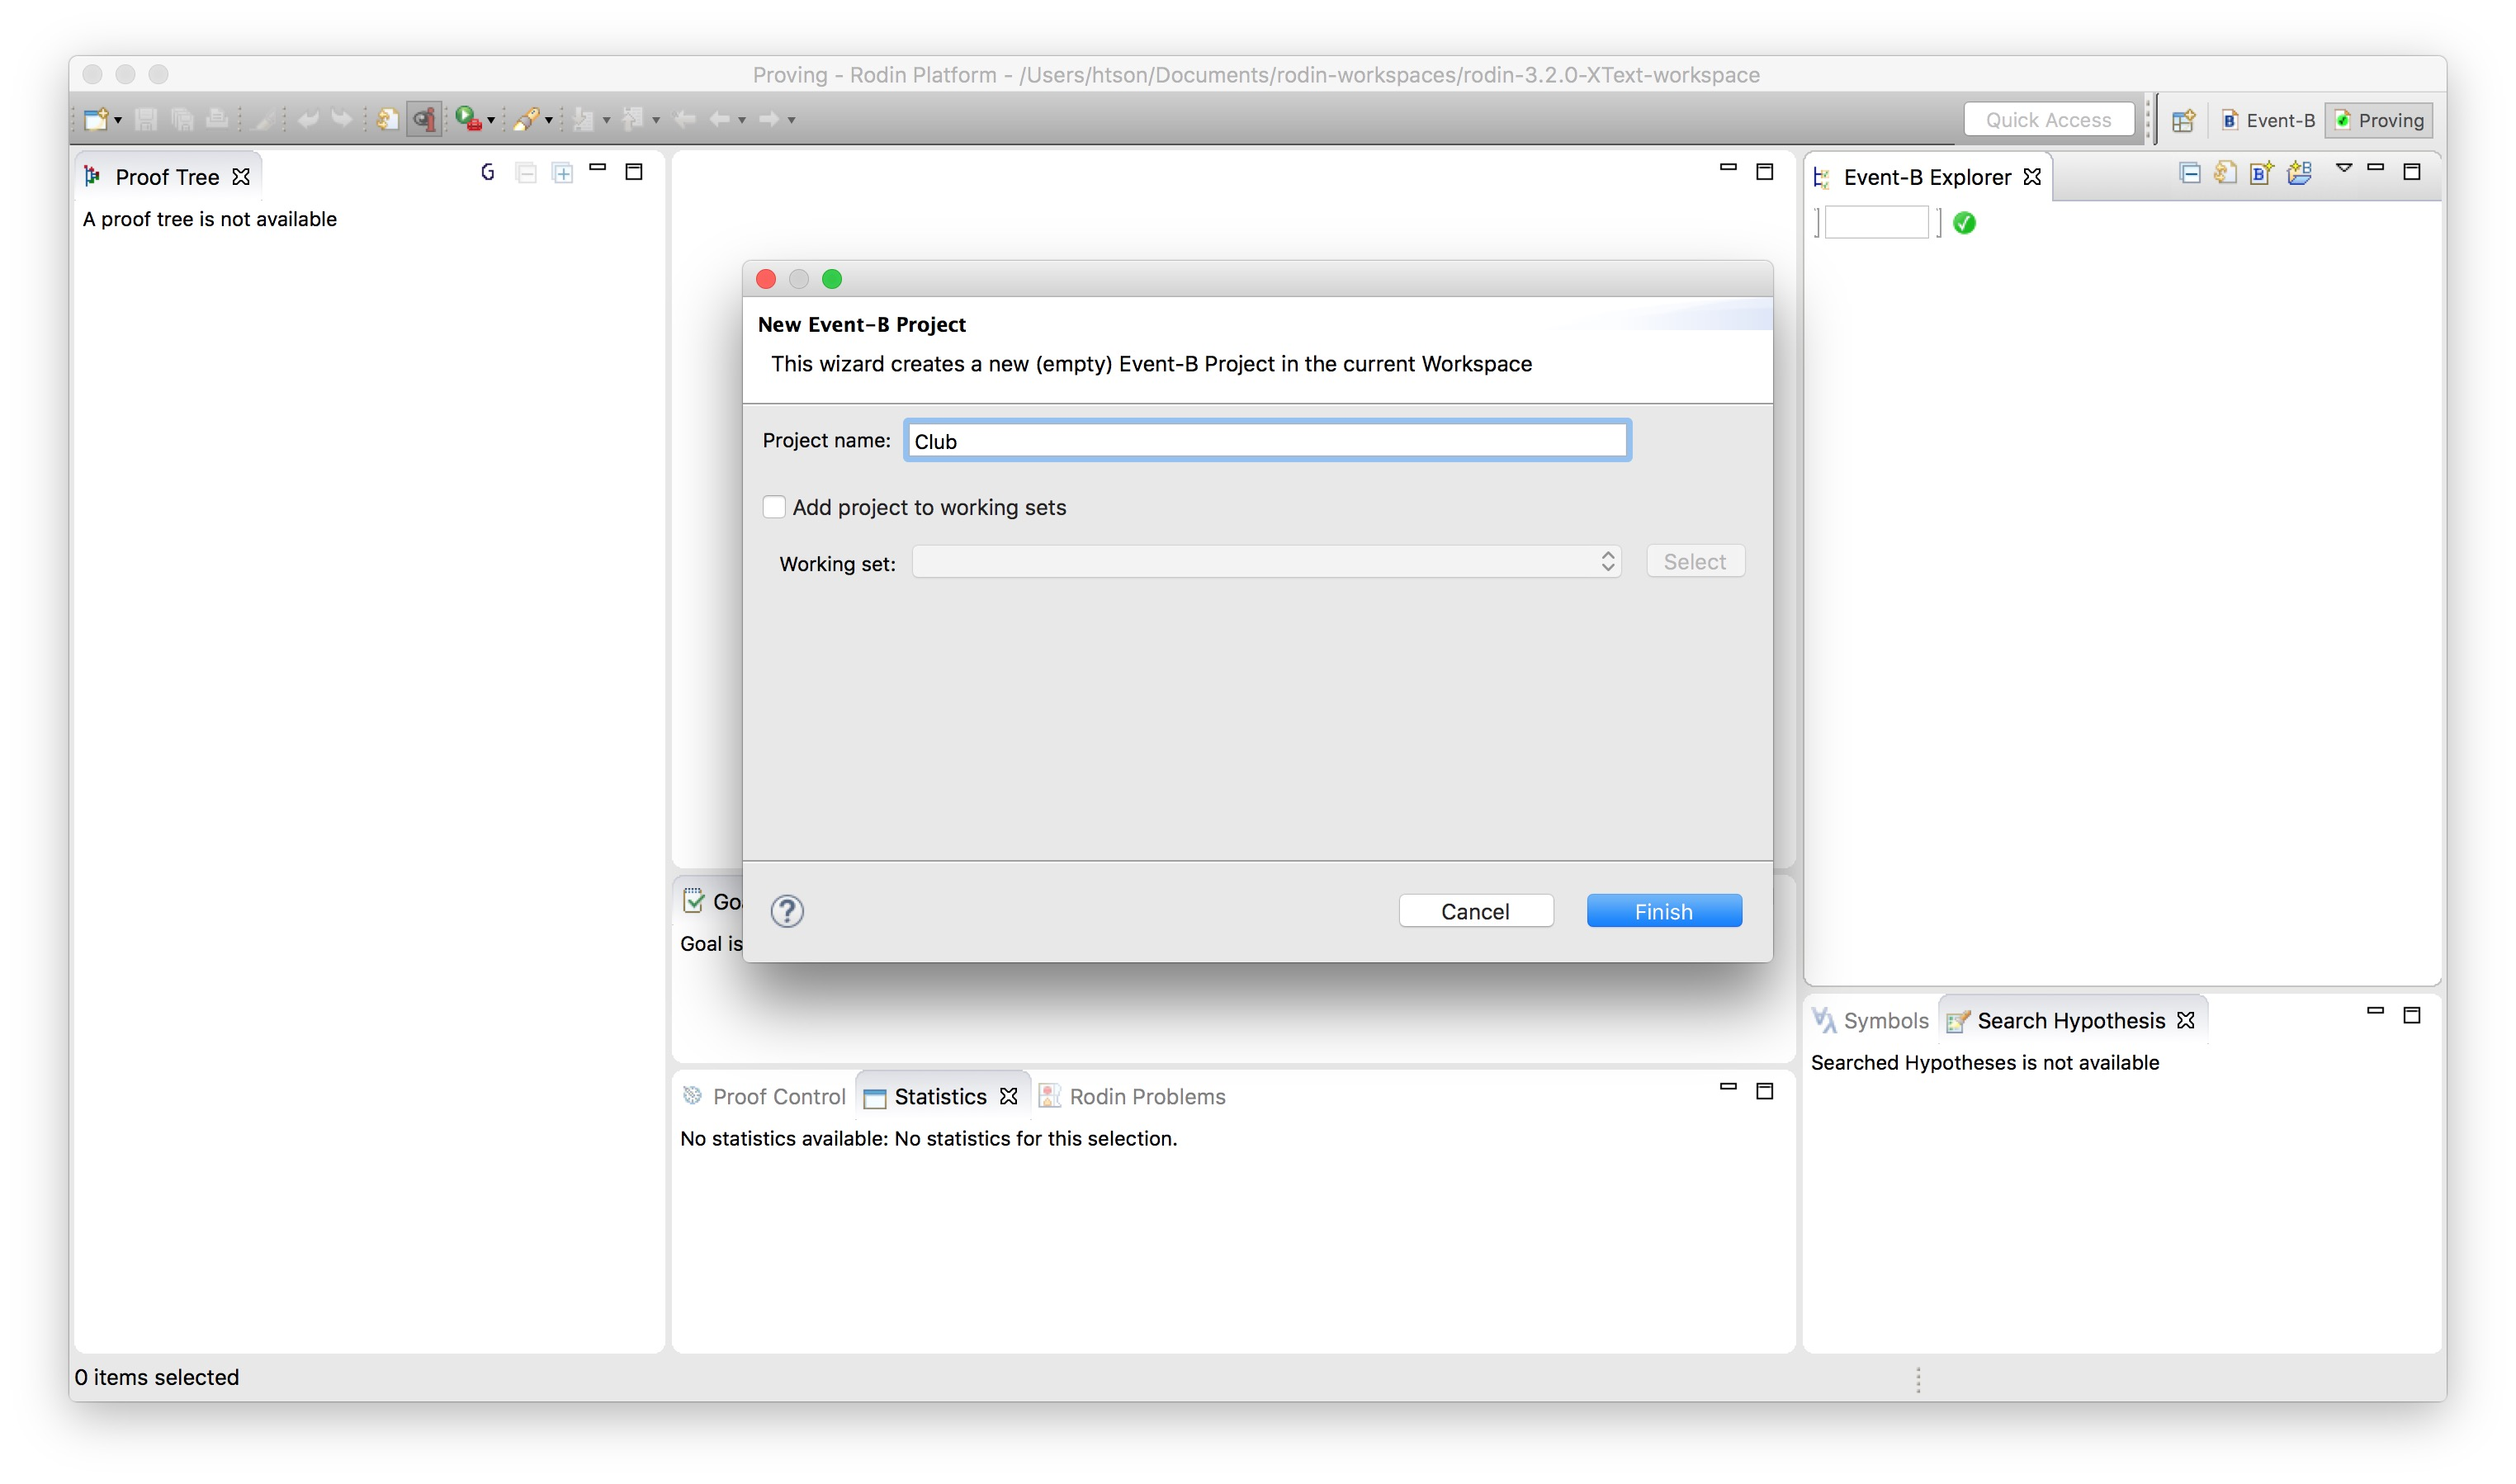
\includegraphics[width=512]{figures/CreateProject}
  \else
  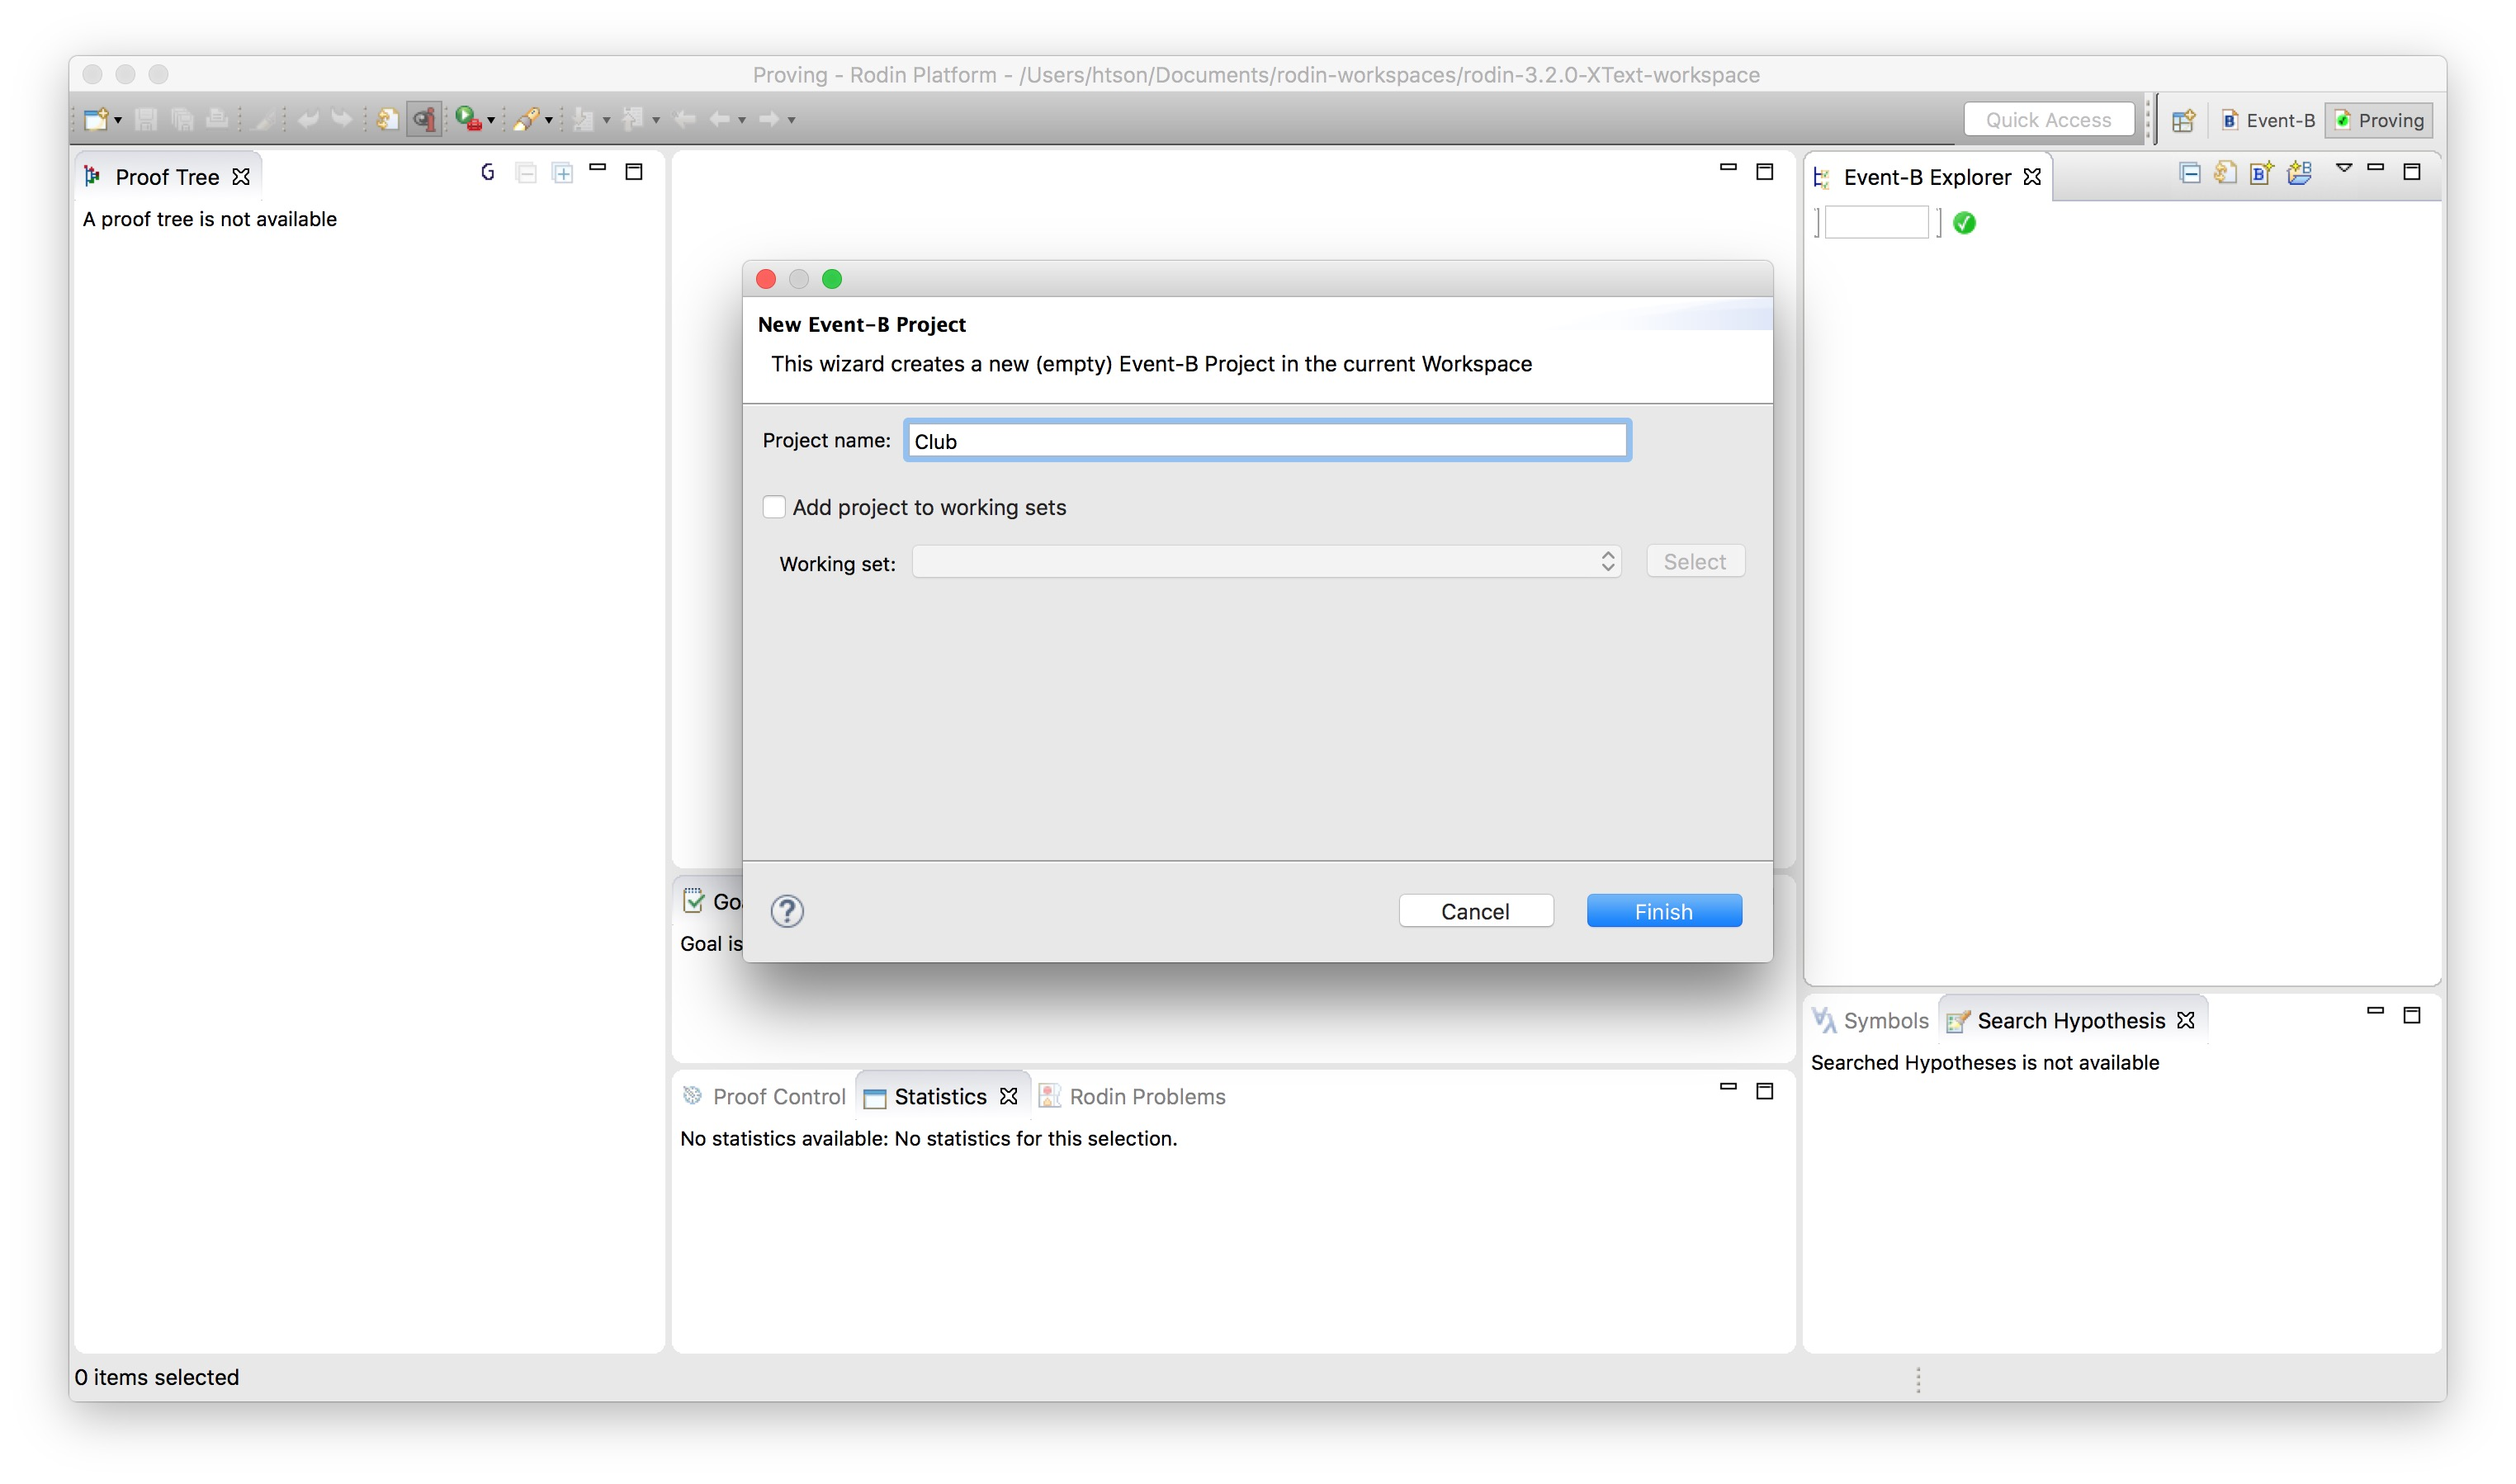
\includegraphics[width=0.9\textwidth]{figures/CreateProject}
  \endif
  \caption{Create Event-B Project called ``Club''}
  \label{fig:CreateProject}
\end{figure}

\end{description}
\textbf{Conclusion} By now, the project ``Club'' should be visible in the Event-B Explorer.


\subsubsection{Task 2. Create a simple XContext coursesCtx.bucx}\label{Sec:SimpleContext}
\textbf{Introduction} The purpose of this task is to create a simple XContext within the newly created project.
\begin{description}
\item[Step 1. Create a new XContext coursesCtx.bucx] Create a new XContext named ``coursesCtx.bucx'' using the \emph{New File wizard} (see Figure~\ref{fig:CreateCoursesCtx}).
         \textbf{Important}: A pop-up dialog will be displayed asking to convert the ``Club''
         project to XText project, please answer \textbf{Yes} (see Figure~\ref{fig:ConvertToXText}).
\begin{figure}[!htbp]
  \centering
  \ifdef{PLASTEX}
  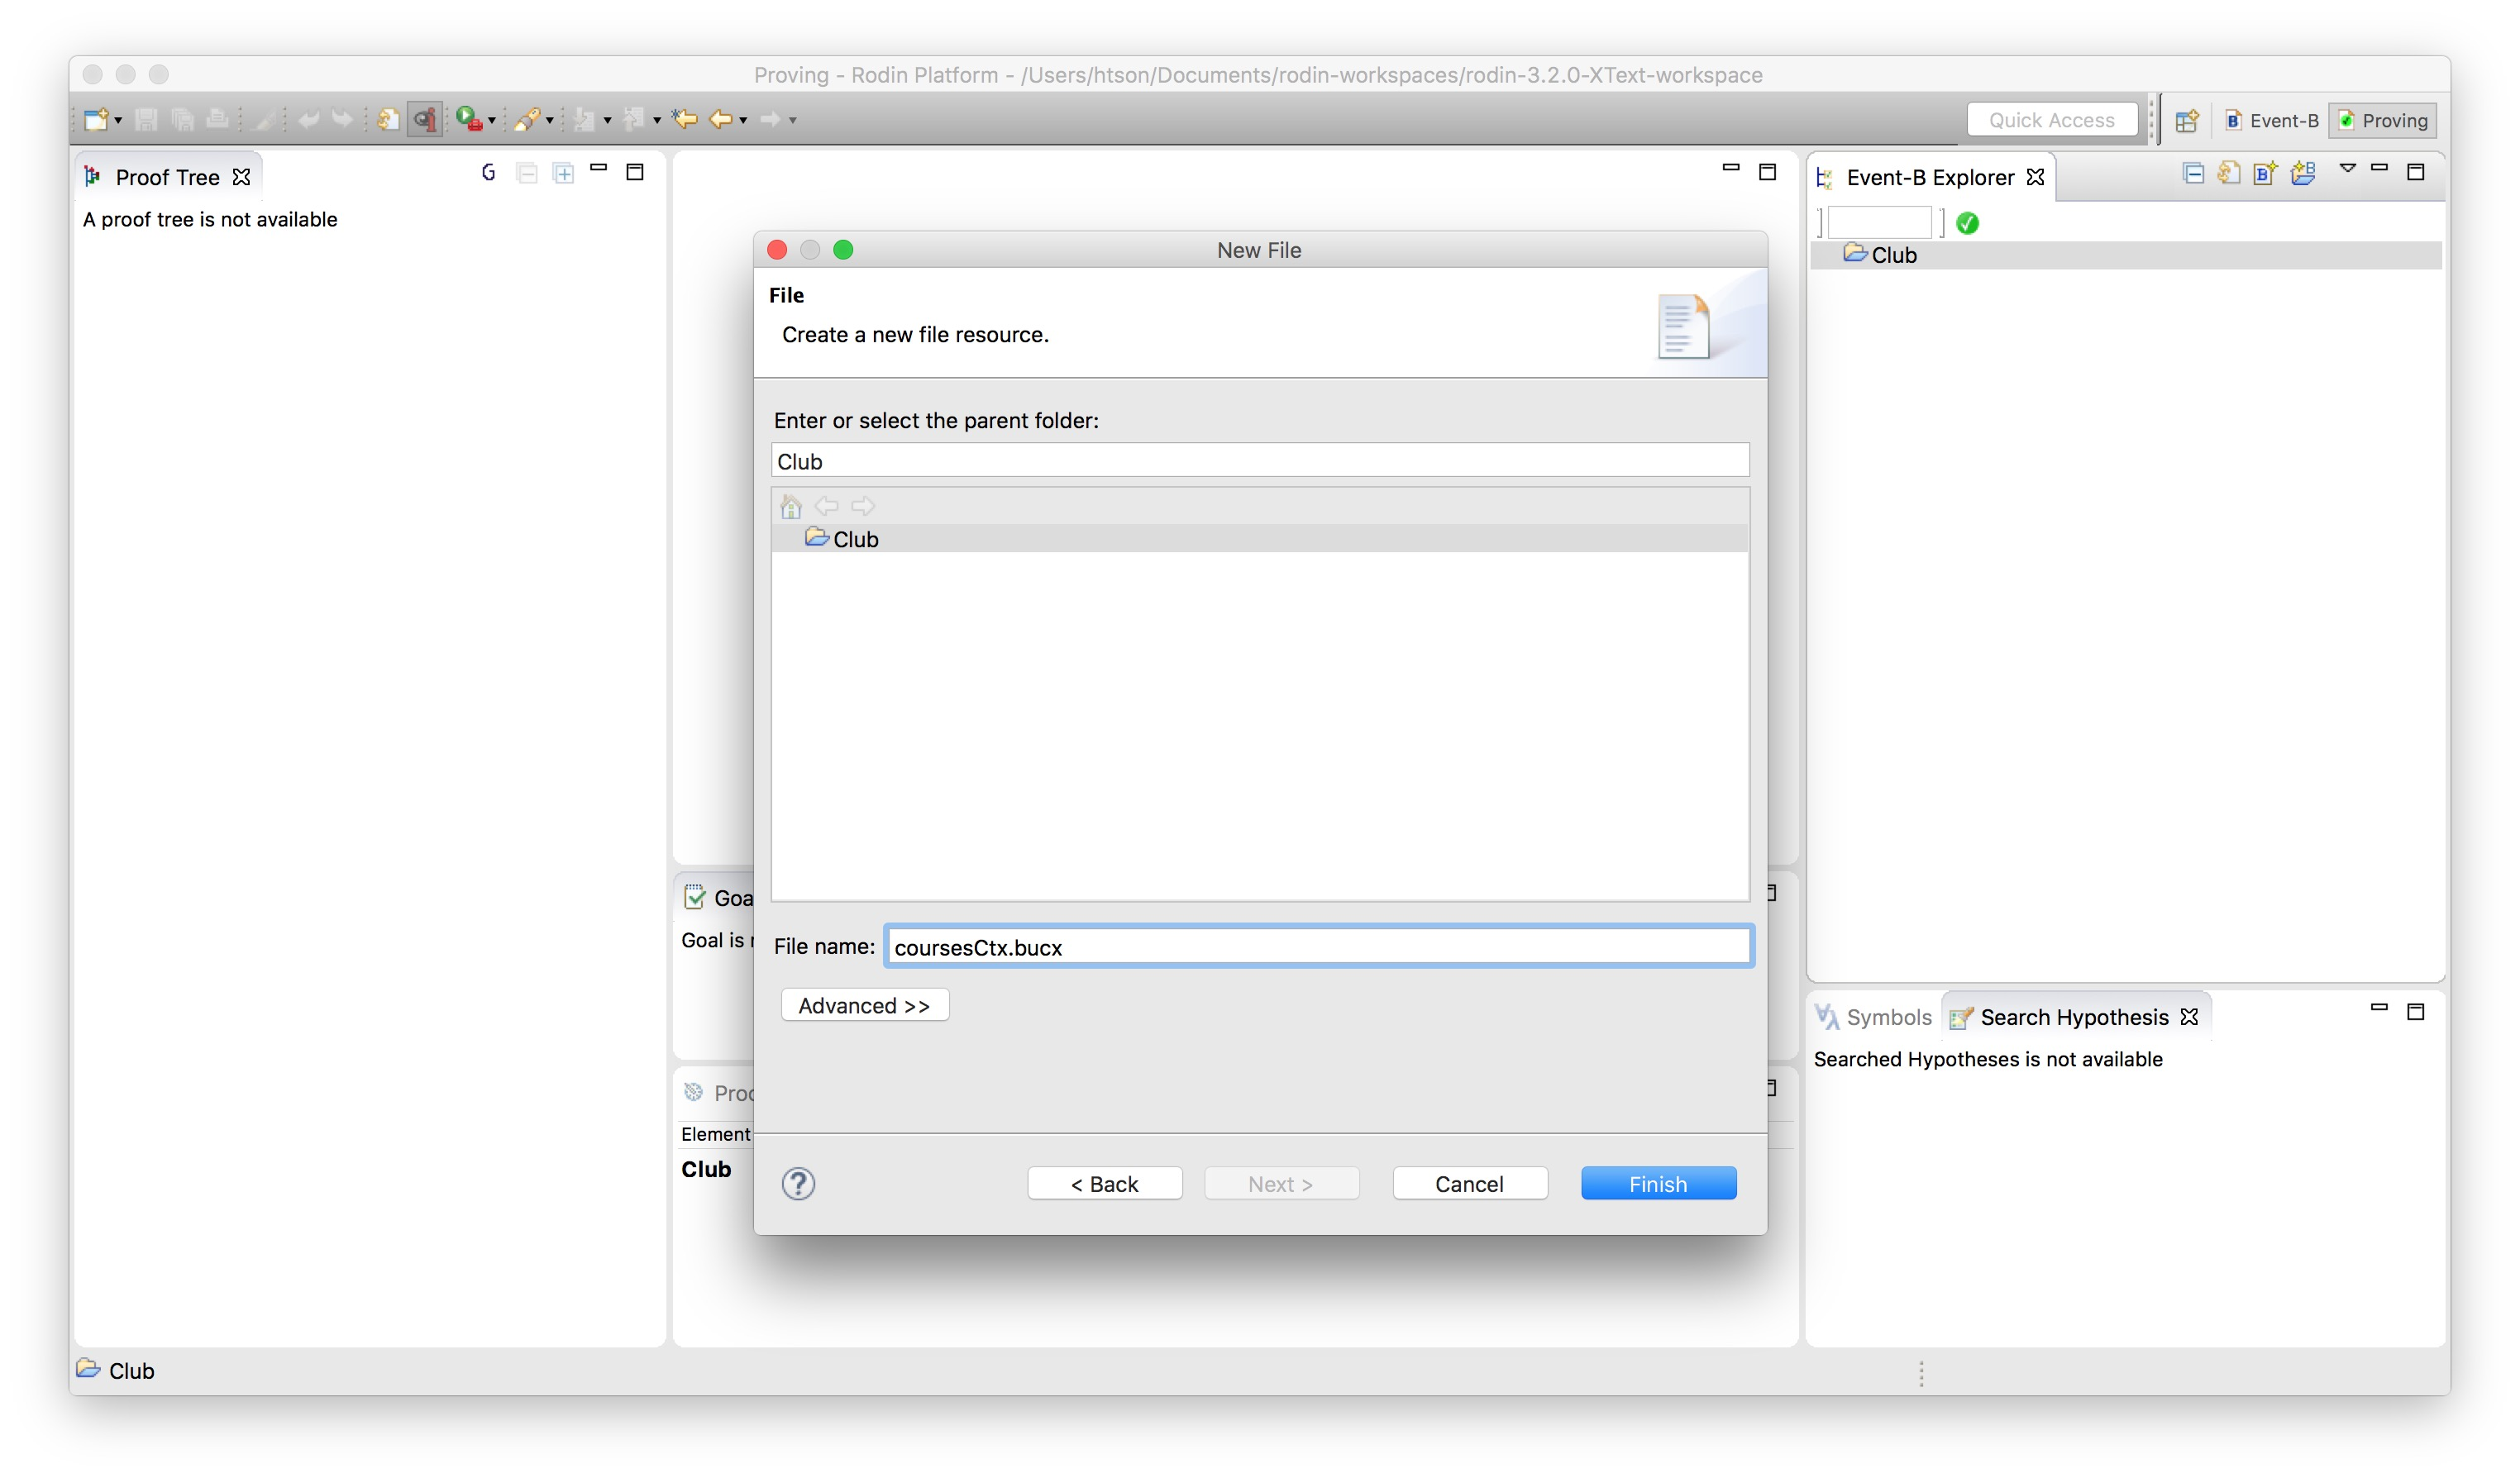
\includegraphics[width=512]{figures/CreateCoursesCtx}
  \else
  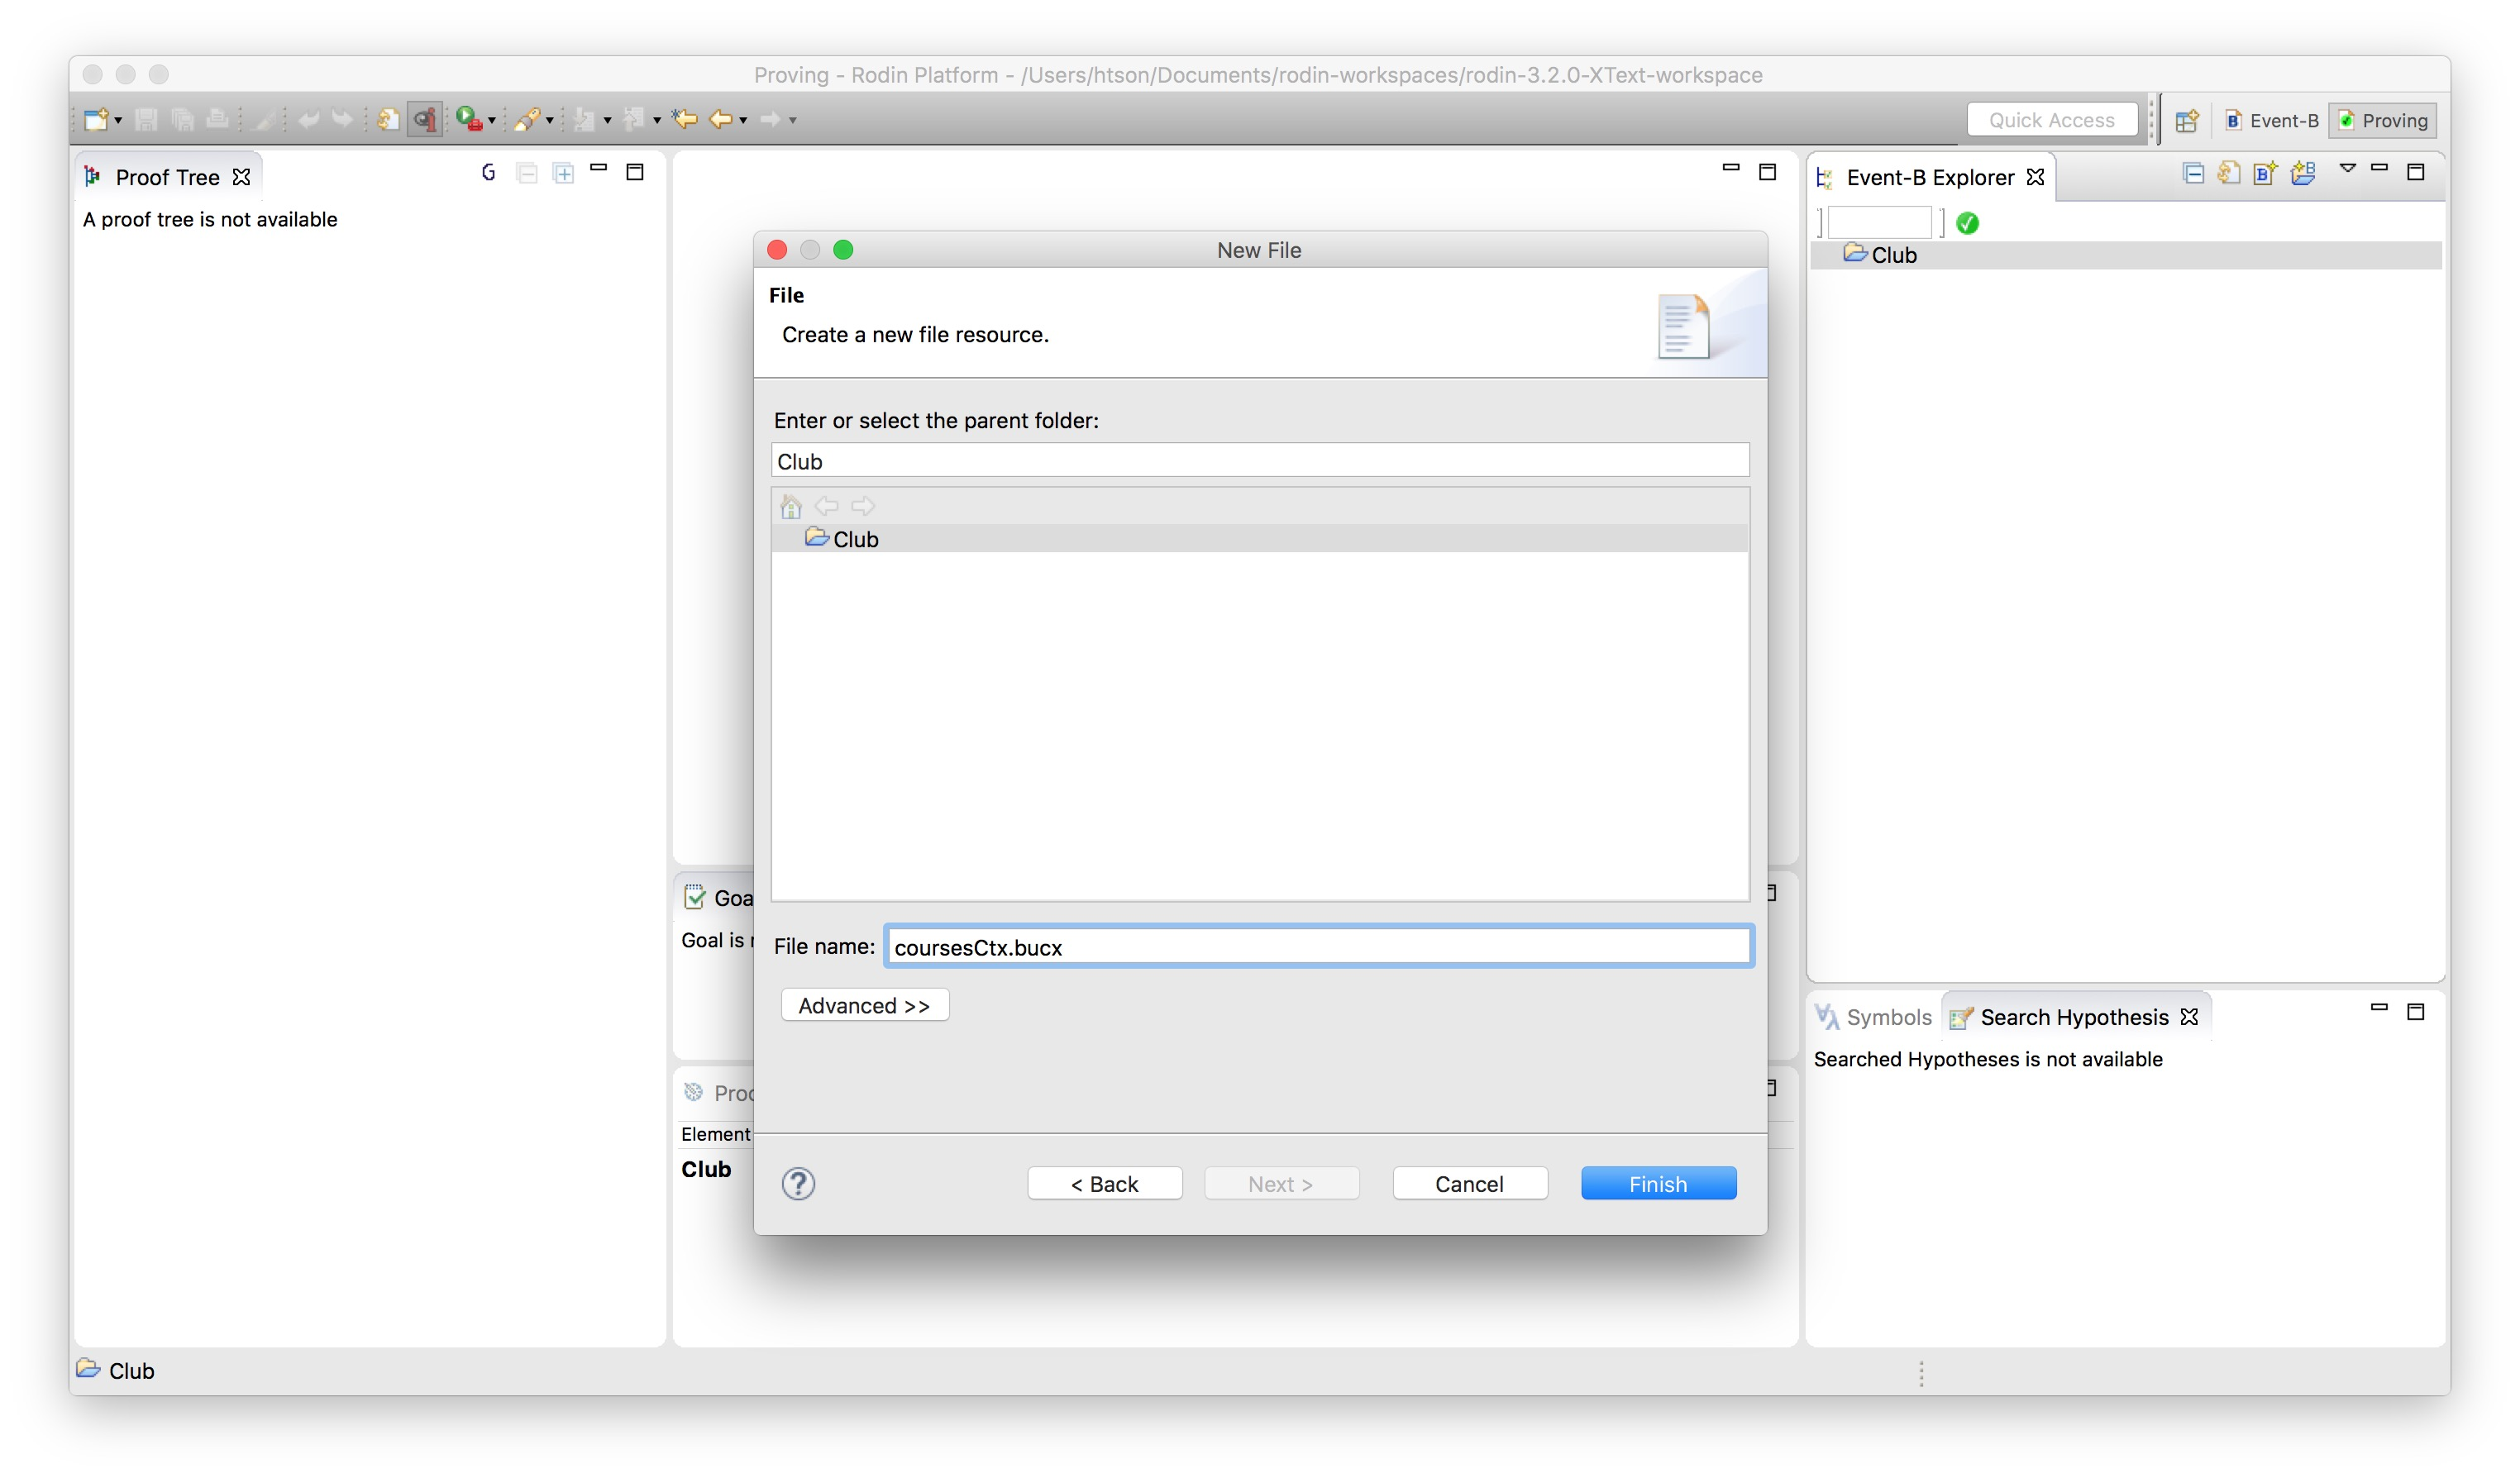
\includegraphics[width=0.9\textwidth]{figures/CreateCoursesCtx}
  \endif
  \caption{Create an XContext called ``coursesCtx.bucx''}
  \label{fig:CreateCoursesCtx}
\end{figure}
\begin{figure}[!htbp]
  \centering
  \ifdef{PLASTEX}
  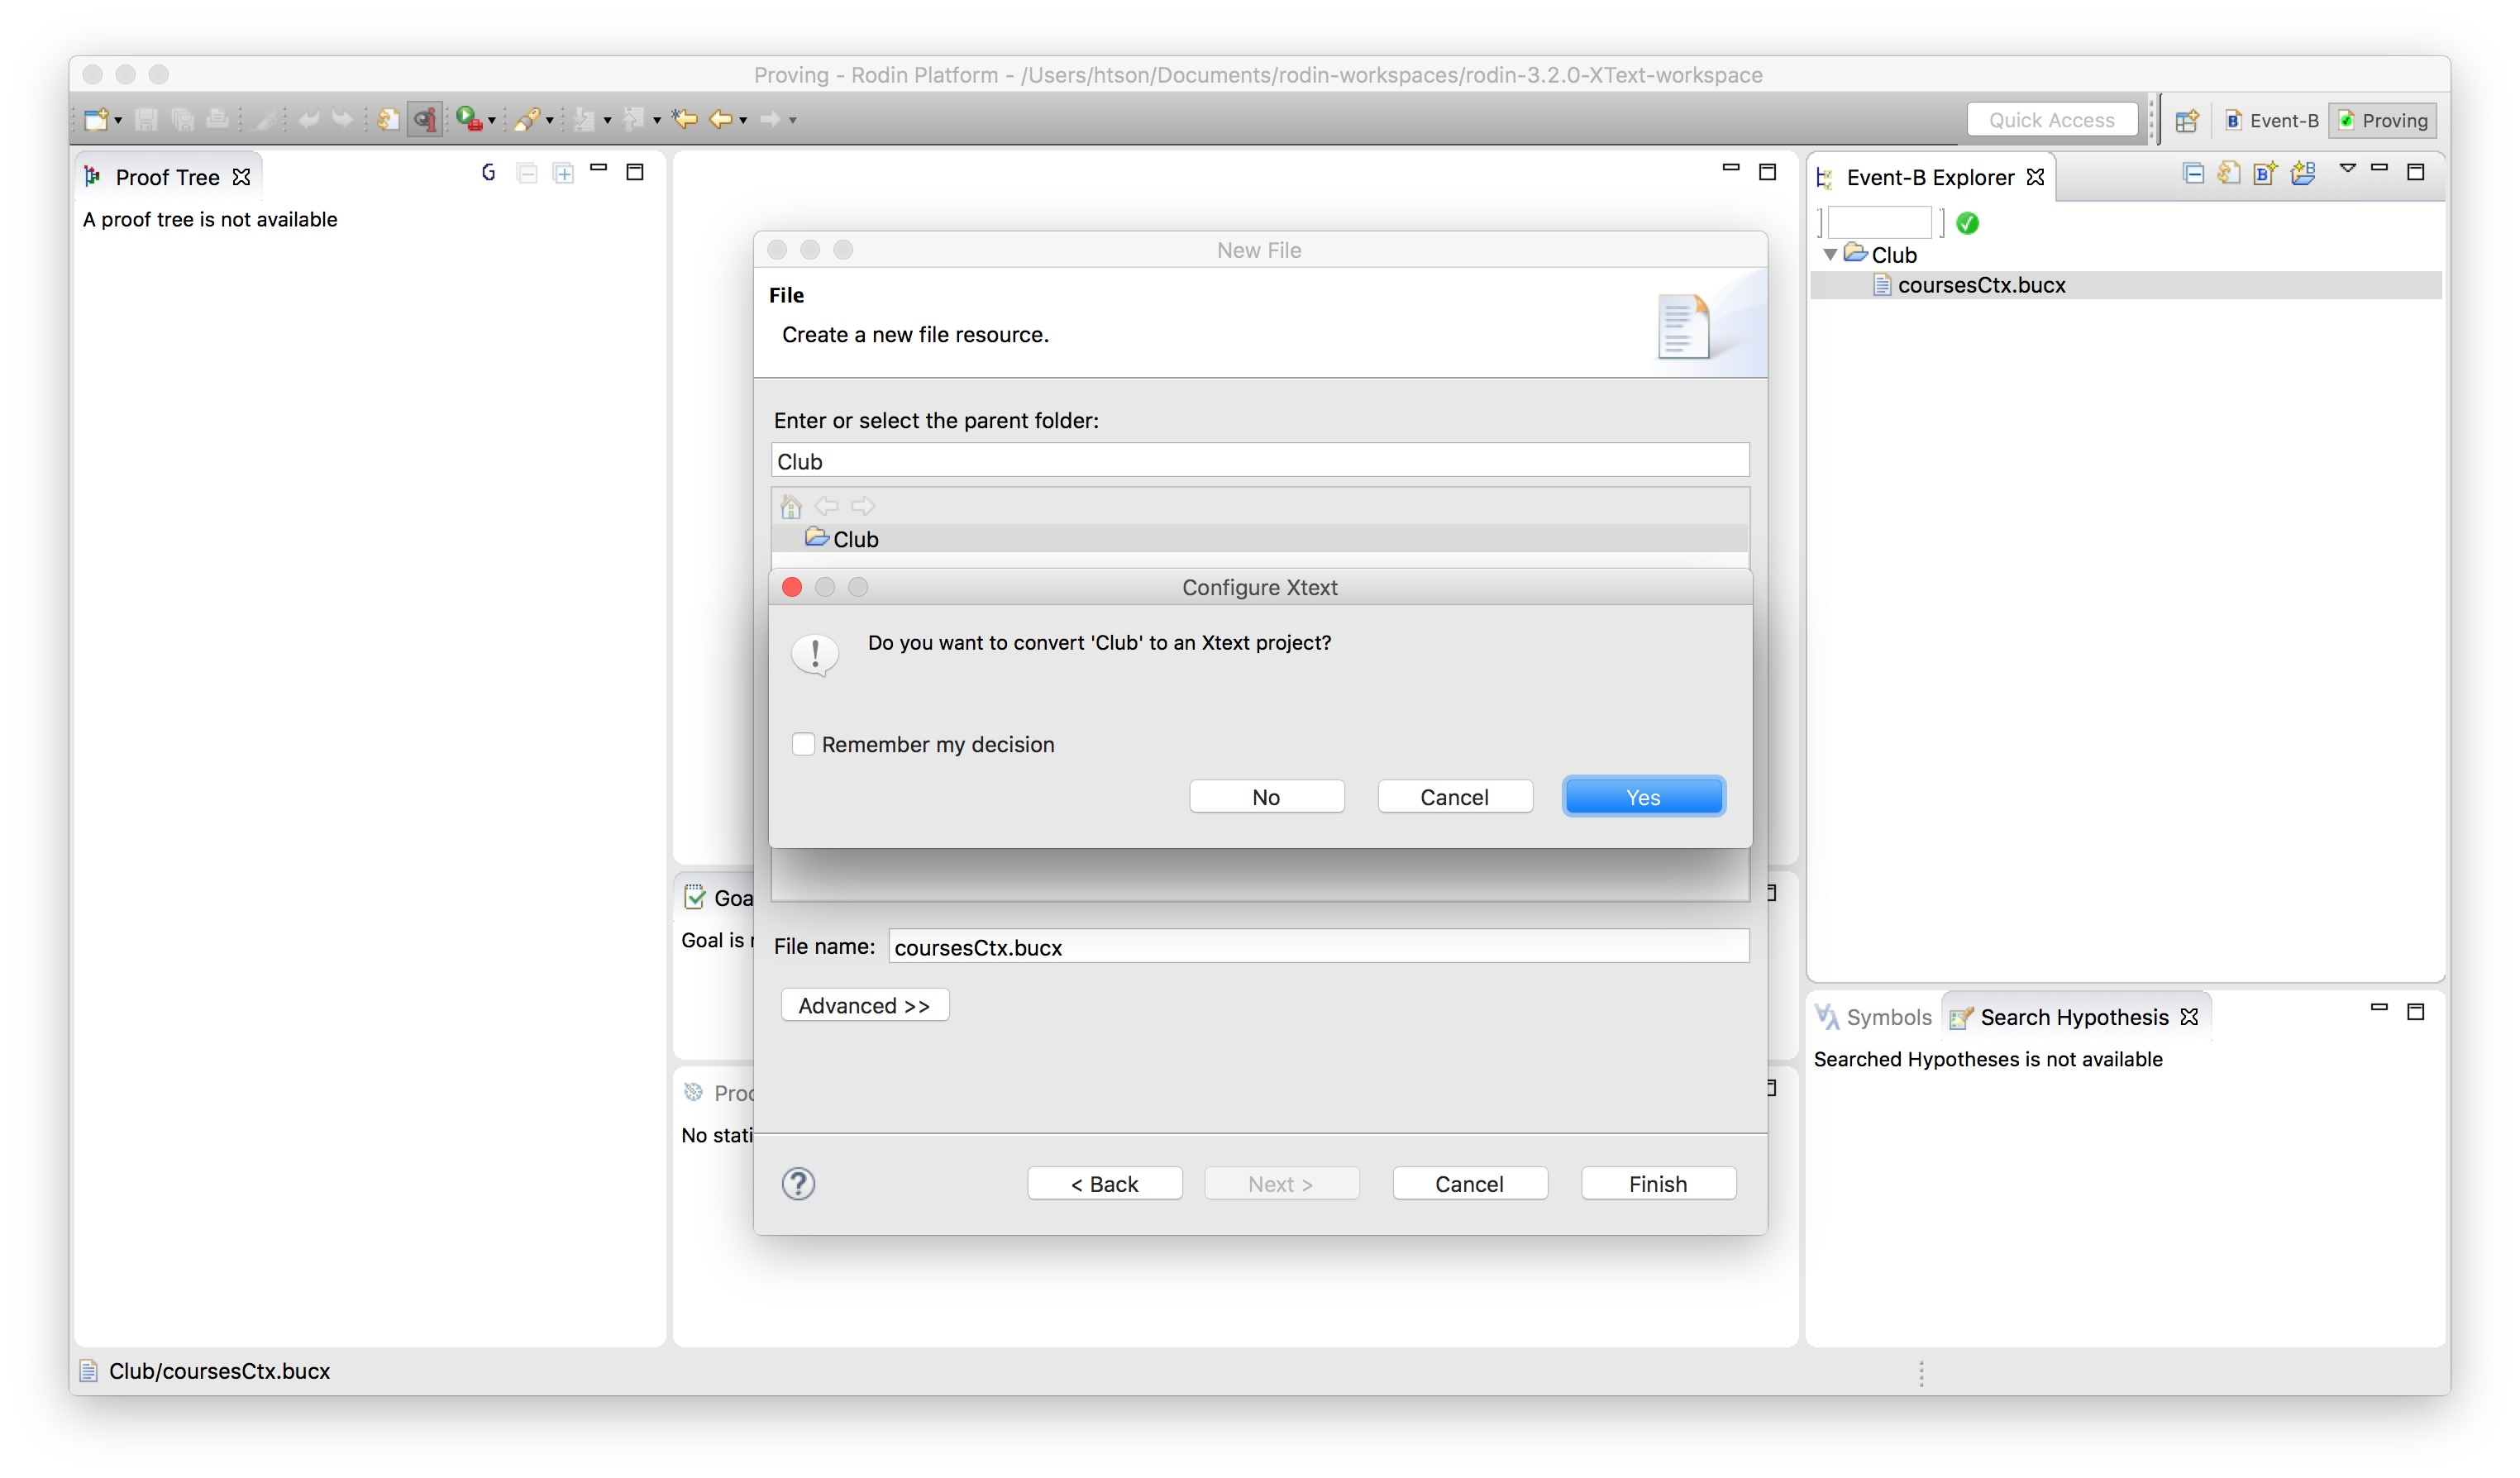
\includegraphics[width=512]{figures/ConvertToXText}
  \else
  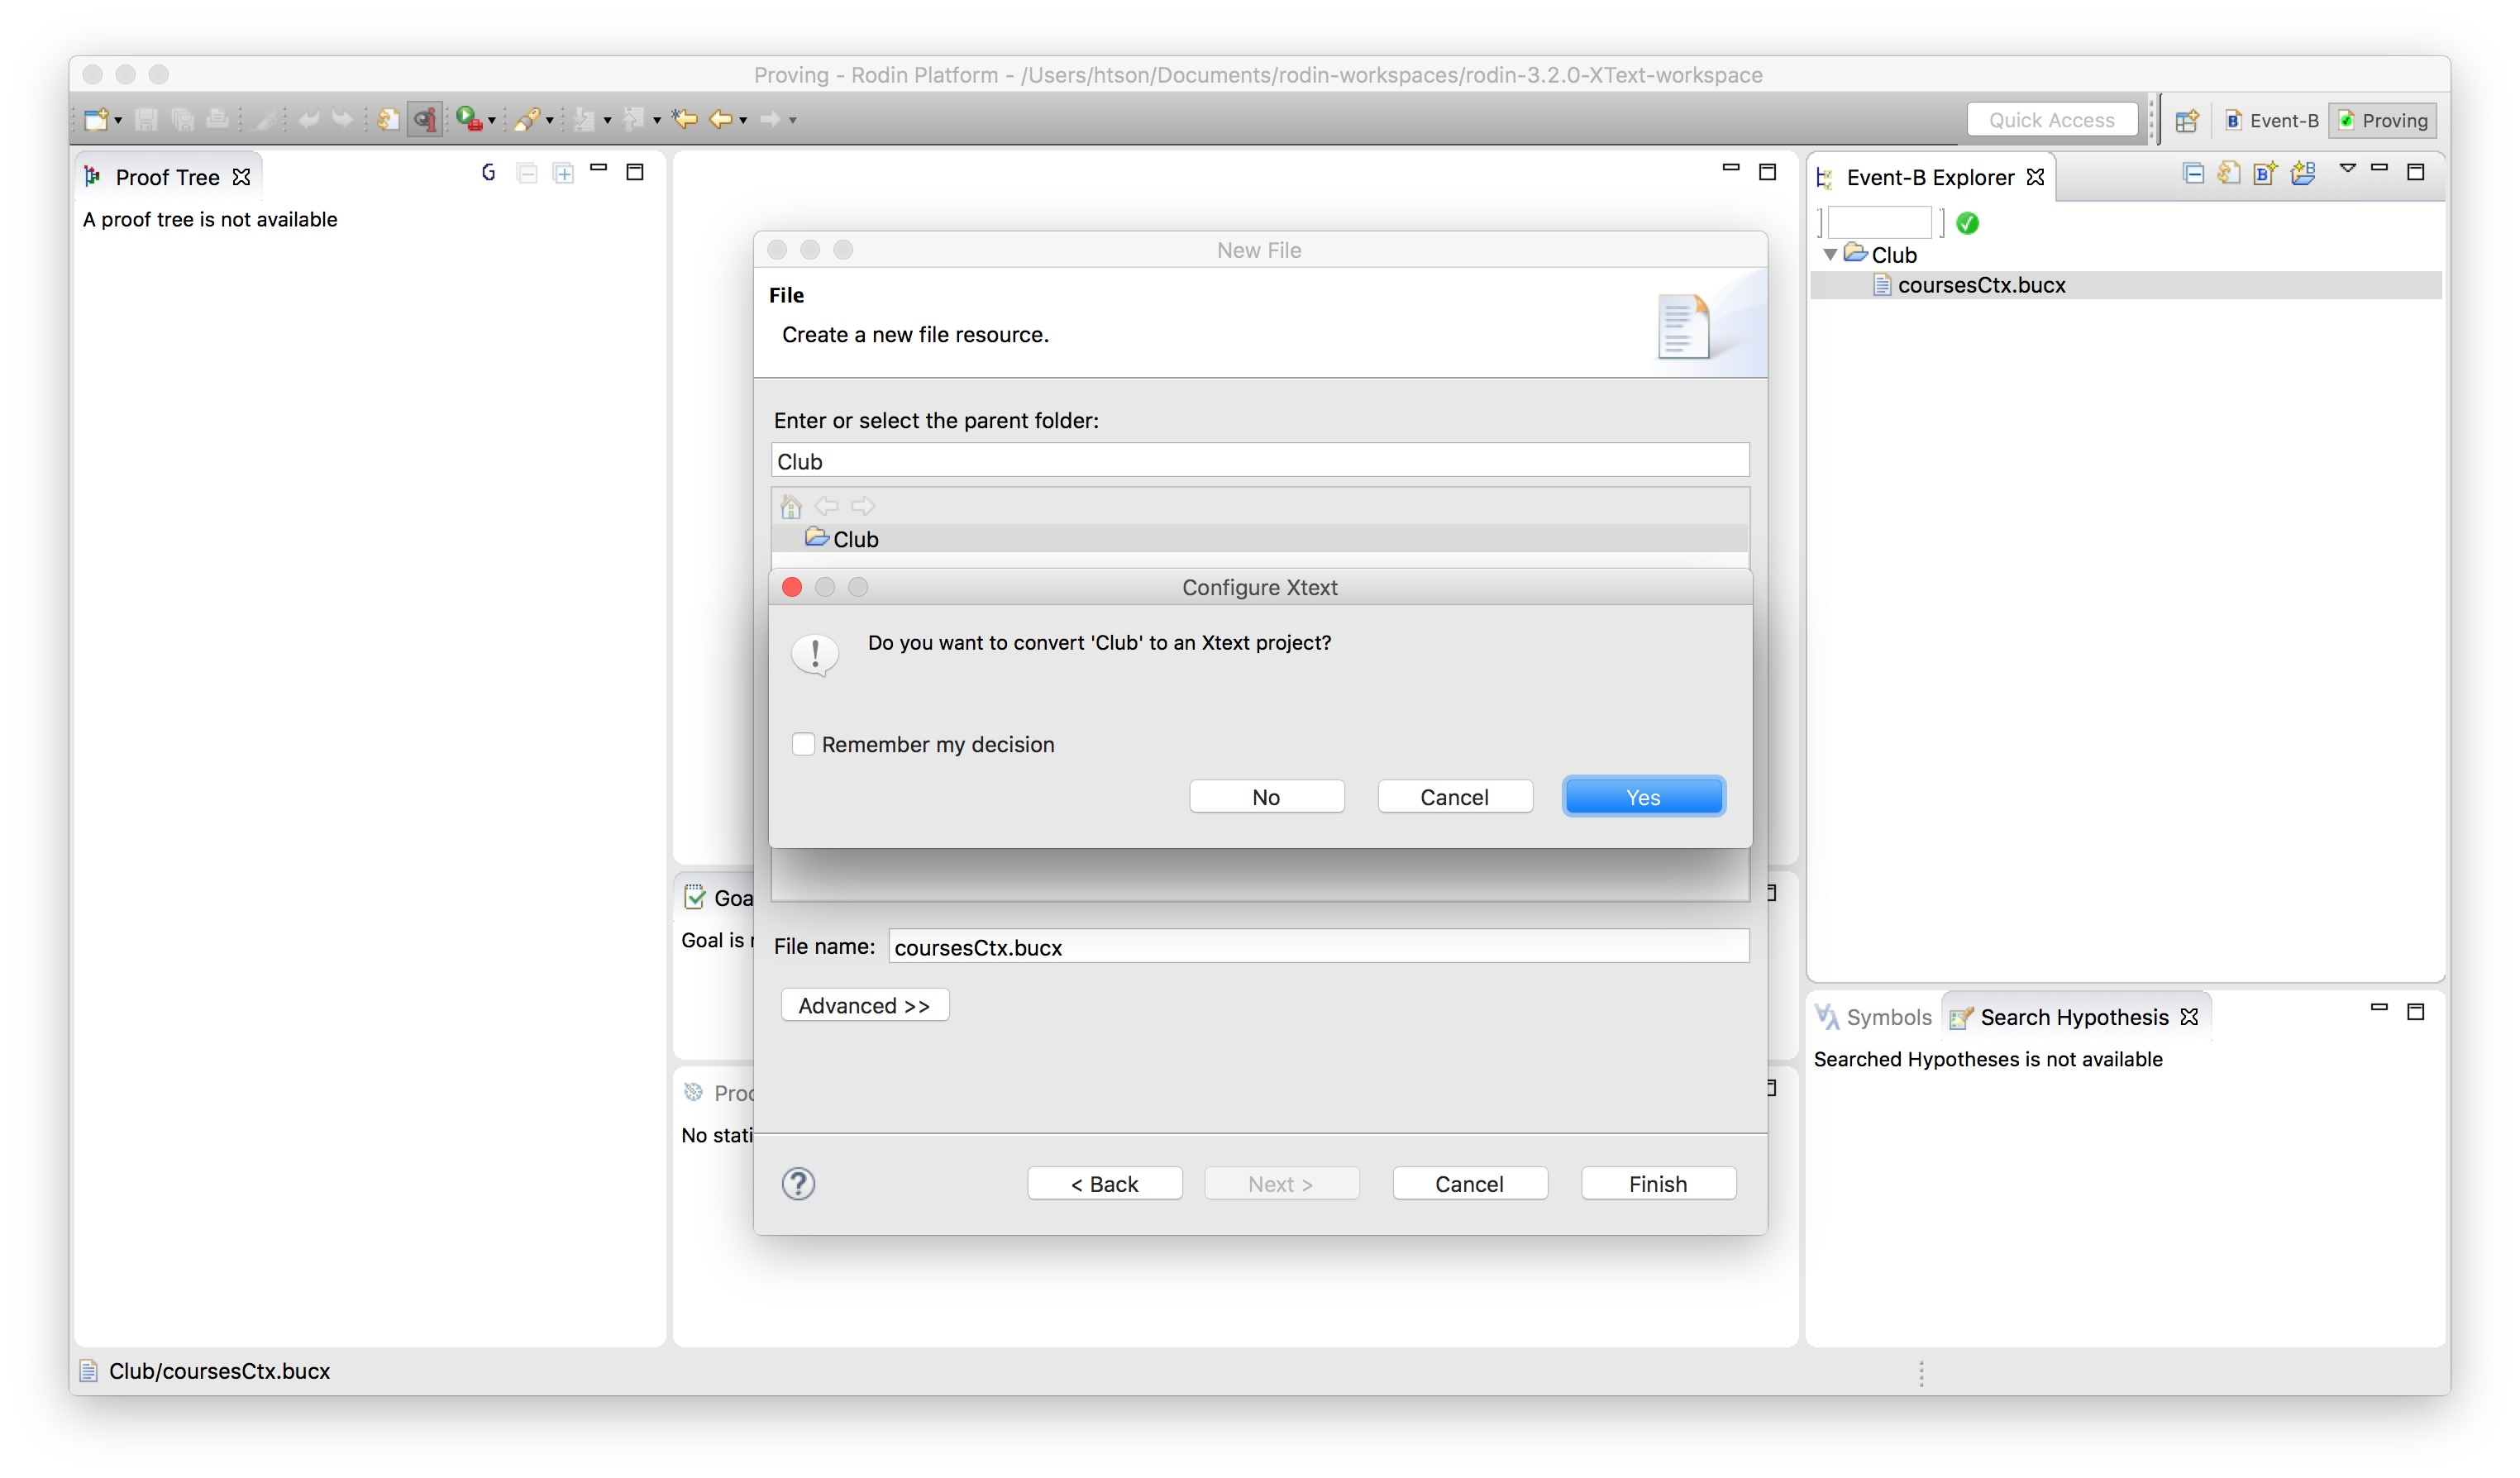
\includegraphics[width=0.9\textwidth]{figures/ConvertToXText}
  \endif
  \caption{Convert ``Club'' to XText project}
  \label{fig:ConvertToXText}
\end{figure}

\item[Step 2. Set the content of courseCtx.bucx] Set the content of ``coursesCtx.bucx'' as follows.
  \begin{center}
    \begin{Bcode}
      \ifdef{PLASTEX}
      \Bcontext{} coursesCtx\\
      \Bsets{} CRS\\
      \Bconstants{} m\\
      \Baxioms\\
      @axm0_1: finite(CRS)\\
      @axm0_2: m ∈ ℕ1\\
      \Btheorem{} @thm0_1: 0 < m \\
      \Bend
      \else
\Bcontext{} coursesCtx\\
\Bsets{} CRS\\
\Bconstants{} m\\
\Baxioms\\
\Btab @axm0\_1: \(\finite(CRS)\)\\
\Btab @axm0\_2: \(m \in \natn\)\\
\Btab \Btheorem{} @thm0\_1: \(0 < m\)\\
\Bend
       \endif
    \end{Bcode}
  \end{center}
  \textbf{Important}: In order to typeset Event-B mathematical symbol, e.g., \ifdef{PLASTEX} ℕ1 \else $\natn$ \endif, one can use content assist. For example, typing \texttt{NAT} and invoking content assist (e.g., on Mac OS \texttt{Ctrl+Space}), a dropdown list will appear with options for typesetting \ifdef{PLASTEX} ℕ \else $\nat$ \endif and \ifdef{PLASTEX} ℕ1 \else $\natn$ \endif (See Figure~\ref{fig:NAT1ContentAssist}.
  \begin{figure}[!htbp]
    \centering
    \ifdef{PLASTEX}
    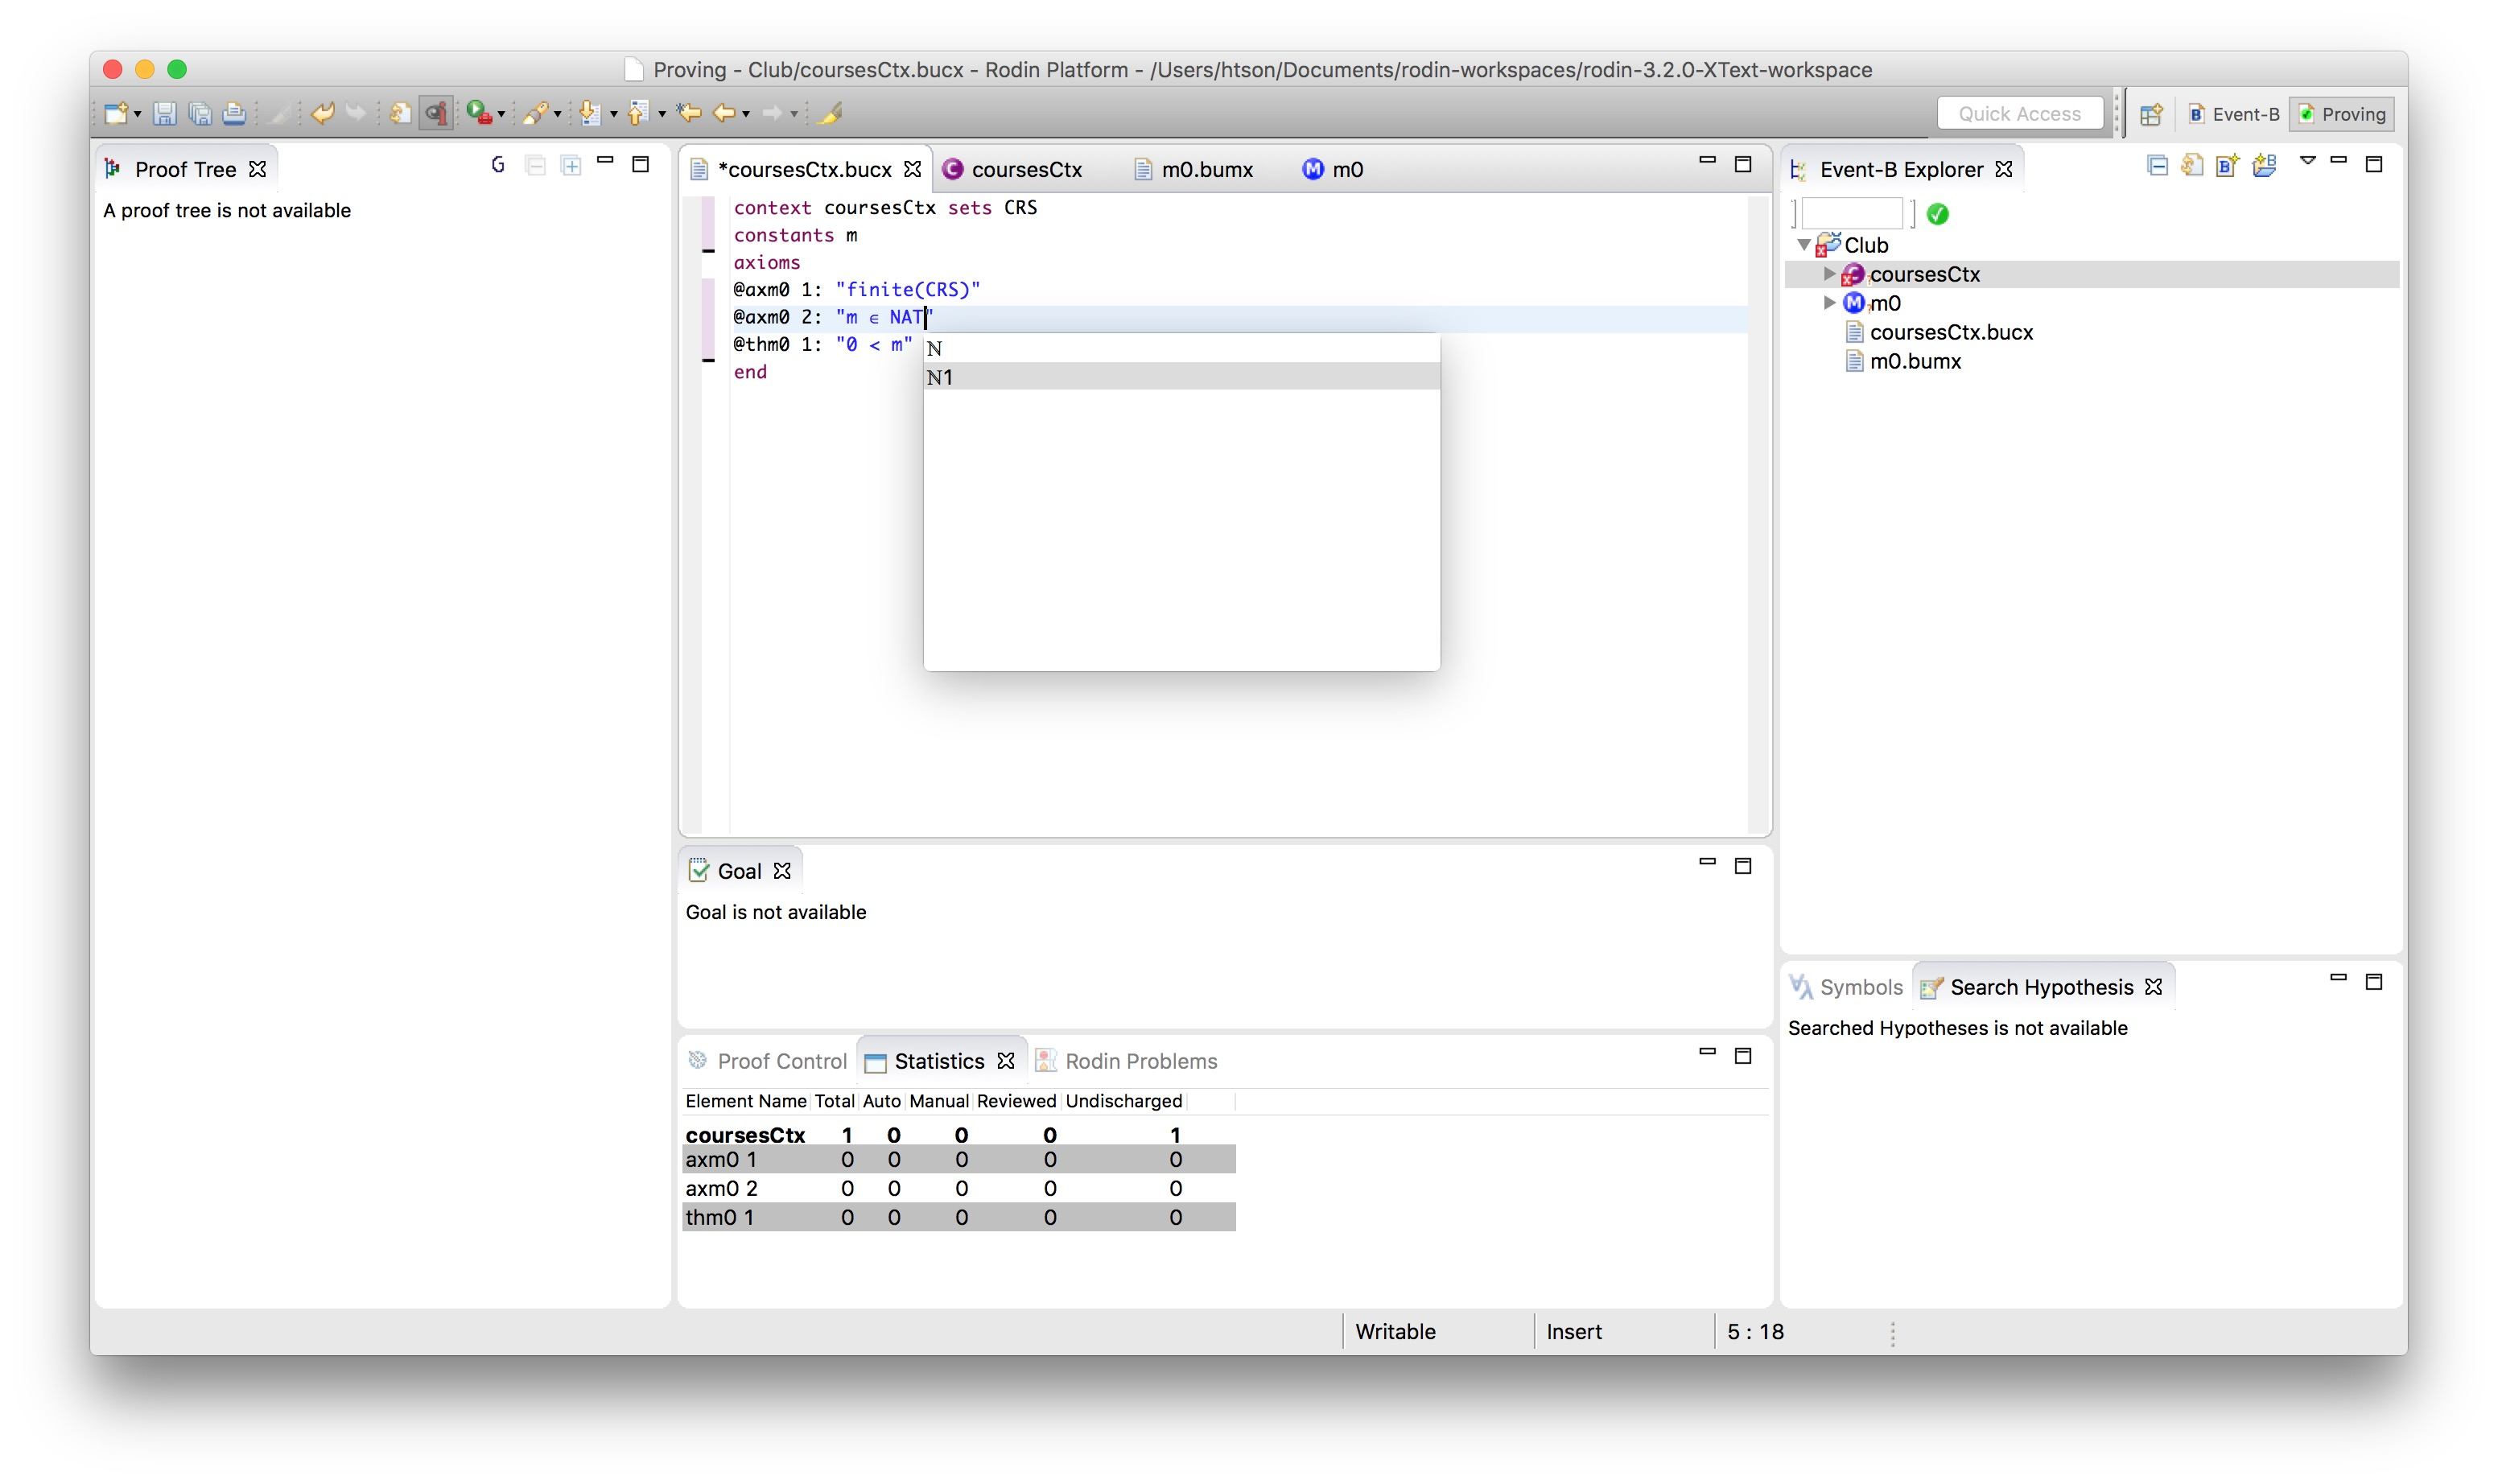
\includegraphics[width=512]{figures/NAT1ContentAssist}
    \else
    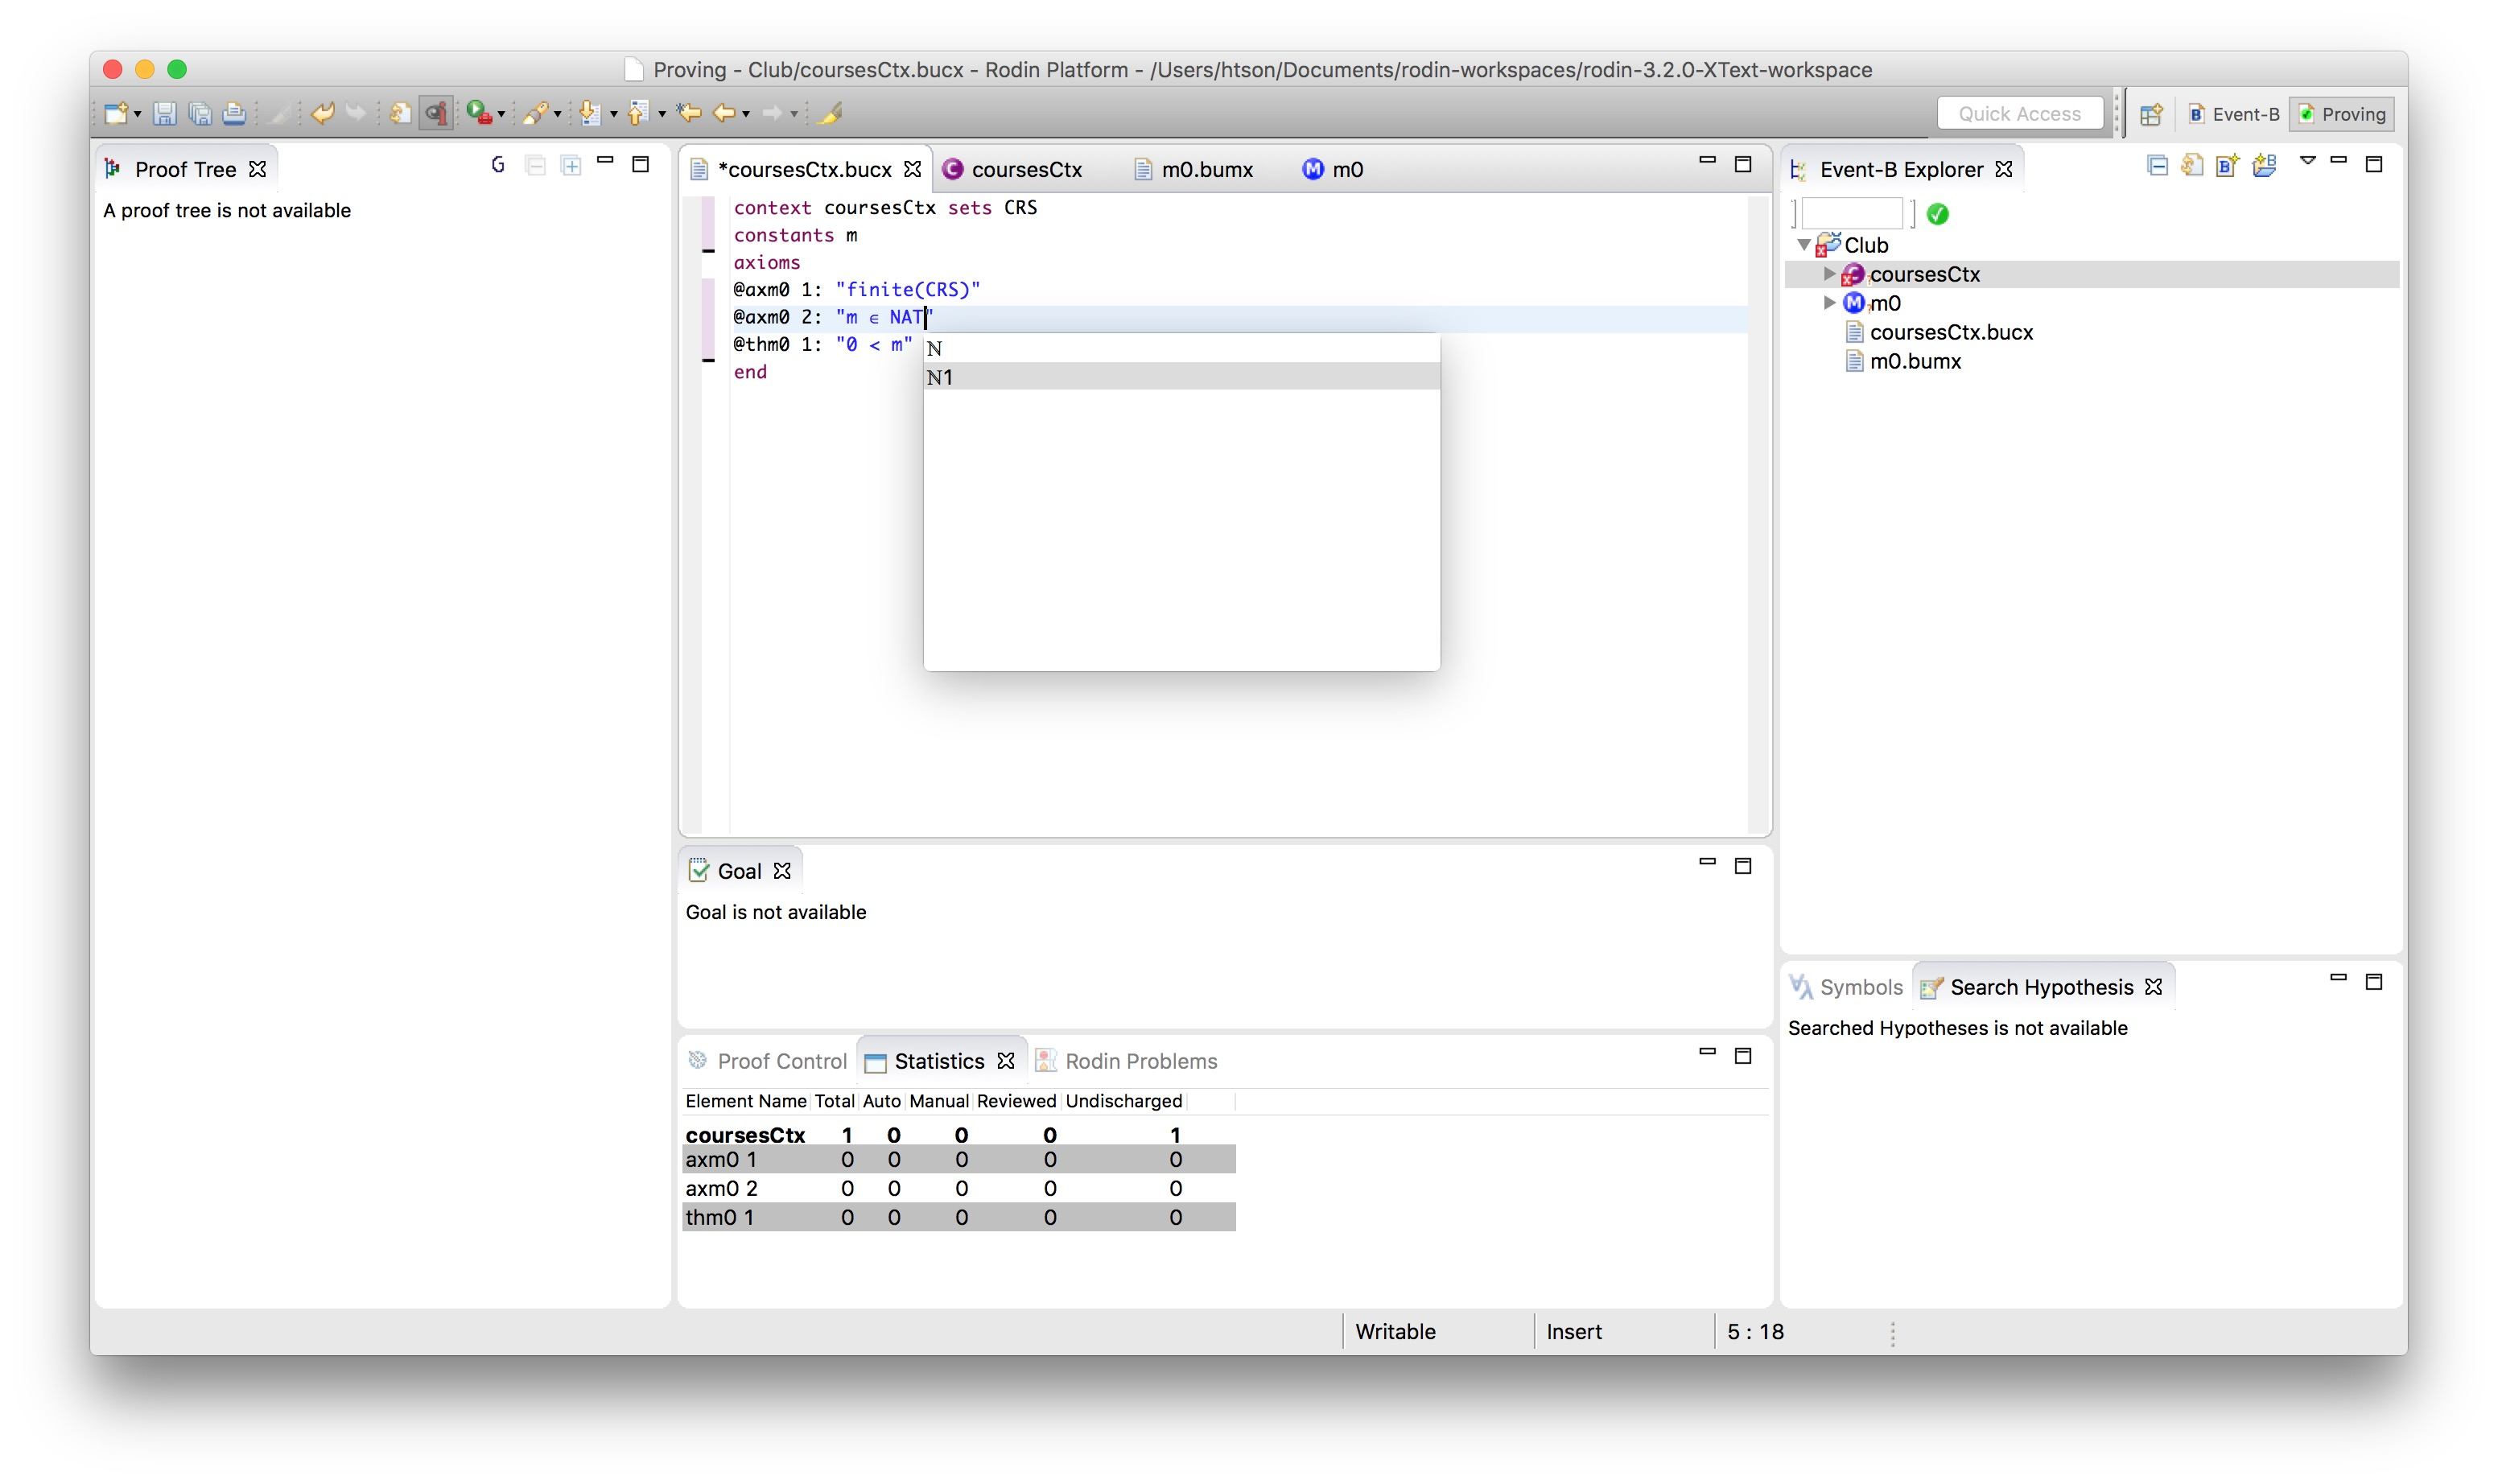
\includegraphics[width=0.9\textwidth]{figures/NAT1ContentAssist}
    \endif
    \caption{Type-setting \ifdef{PLASTEX} ℕ1 \else $\natn$ \endif using Content Assist}
    \label{fig:NAT1ContentAssist}
  \end{figure}

\item[Step 3. Auto-format the code] Automatically format the content of ``coursesCtx.bucx'' using short-cut (e.g., on Mac OS: \texttt{Cmd+Shift+F}).

\item[Step 4. Save the file] \textbf{Save the file ``coursesCtx.bucx''}.
\end{description}
\textbf{Conclusion} By now, the XContext ``coursesCtx.bucx'' and the corresponding Rodin Context ``coursesCtx'' should be visible in the Event-B Explorer (see Figure~\ref{fig:CoursesCtx}). 
  \begin{figure}[!htbp]
    \centering
    \ifdef{PLASTEX}
    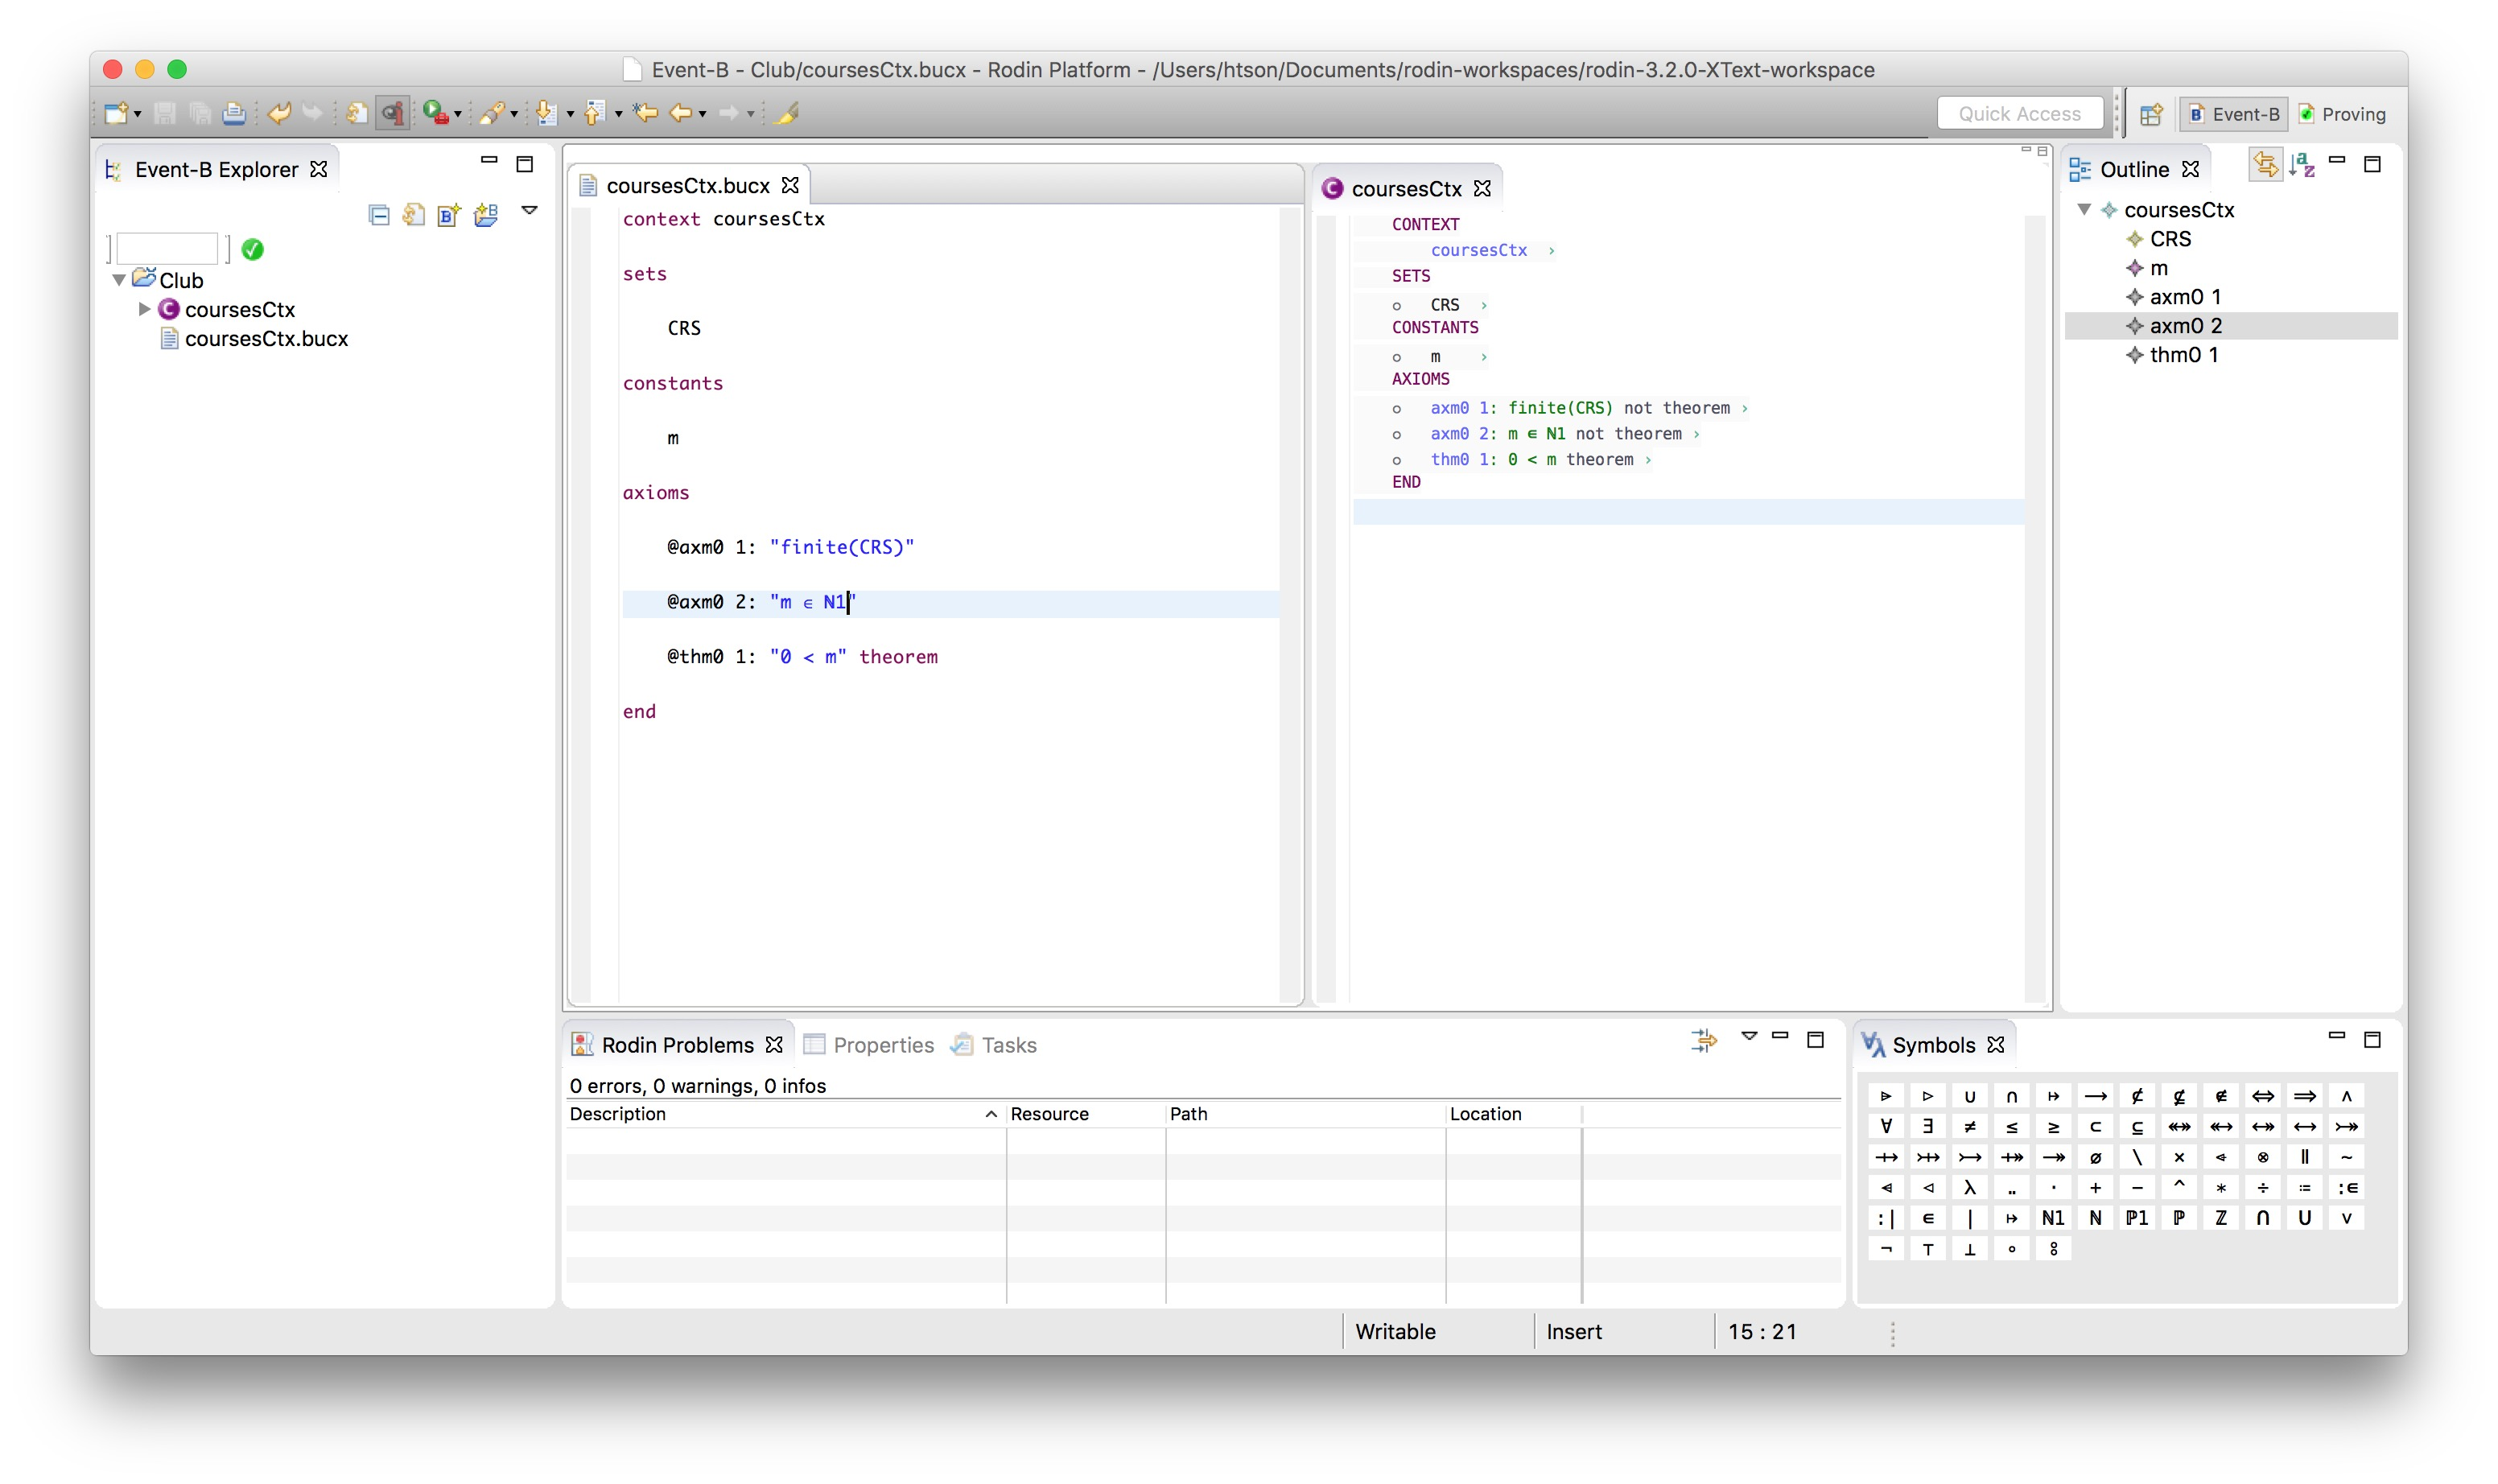
\includegraphics[width=512]{figures/CoursesCtx}
    \else
    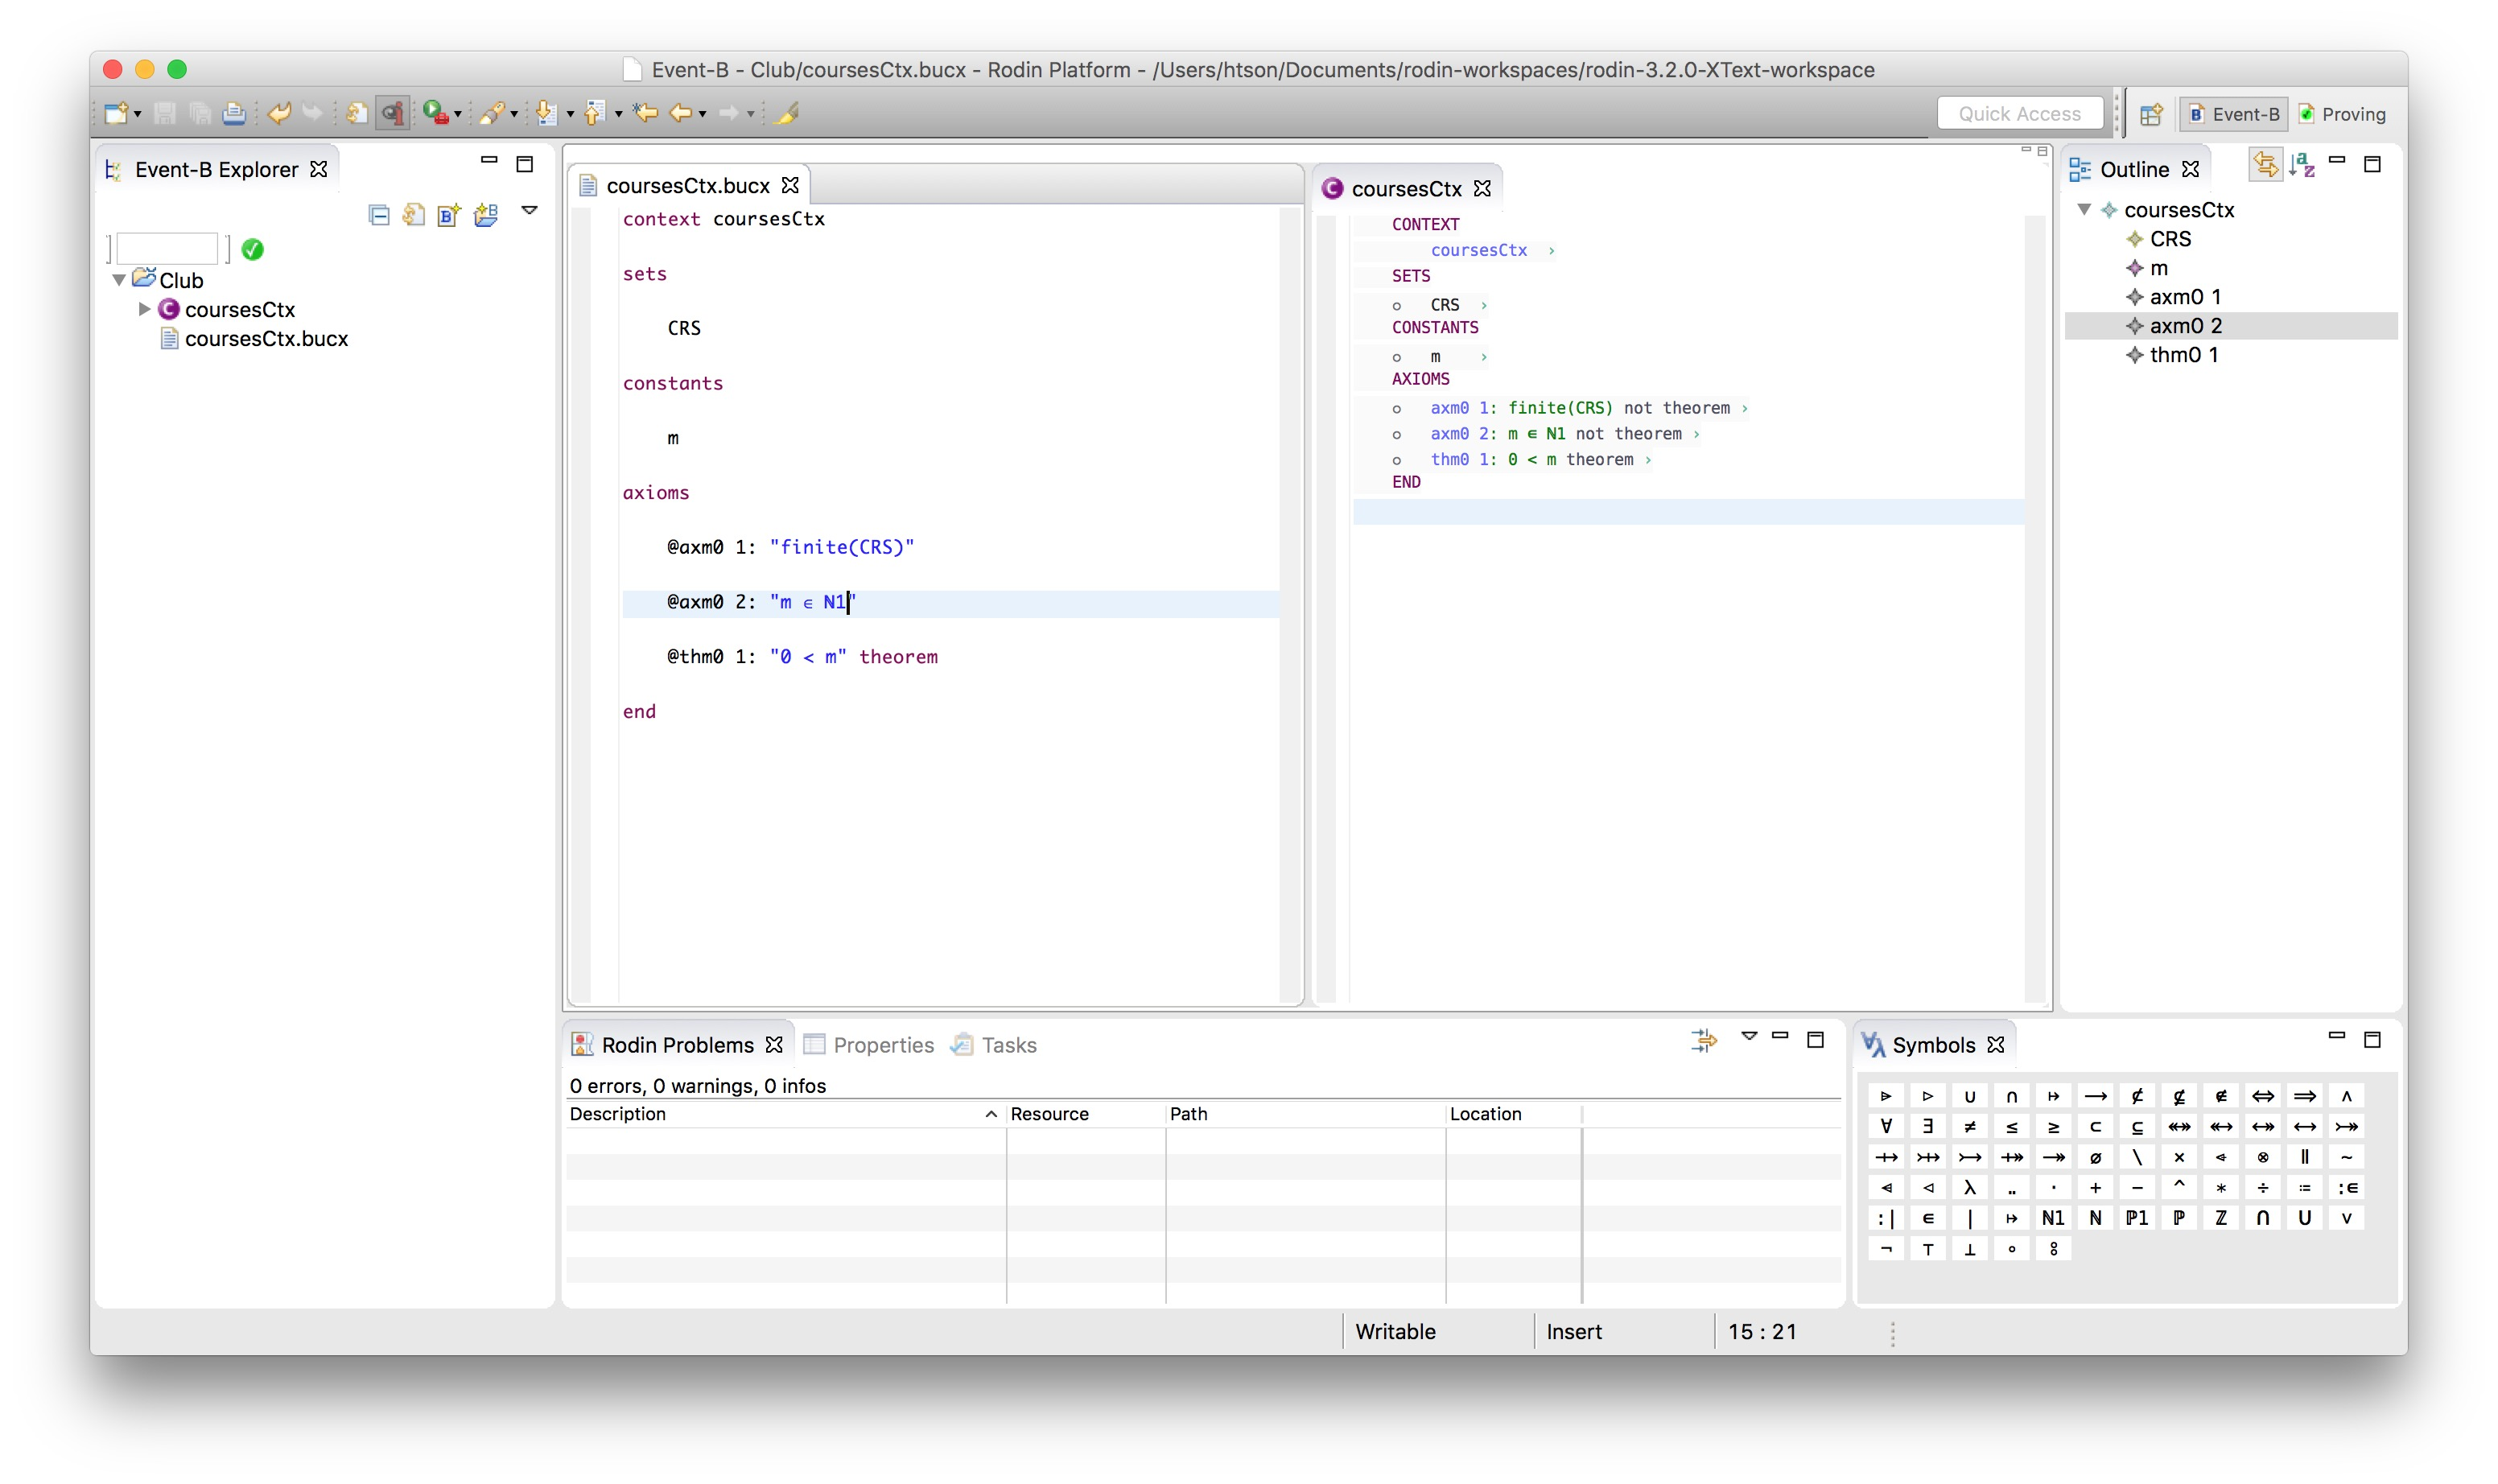
\includegraphics[width=0.9\textwidth]{figures/CoursesCtx}
    \endif
    \caption{The final XContext coursesCtx.bucx}
    \label{fig:CoursesCtx}
  \end{figure}



\subsubsection{Task 4. Create a simple XMachine m0.bumx}\label{CreateMachine}
\textbf{Introduction} The purpose of this task is to create a simple XMachine within the newly created project.

\begin{description}
\item[Step 1. Create a new XMachine m0.bumx] \textbf{Create a new XMachine} named ``m0.bumx'' using the New File wizard (see Figure~\ref{fig:CreateM0}. The newly created file should be opened automatically in an XMachine editor.
  \begin{figure}[!htbp]
    \centering
    \ifdef{PLASTEX}
    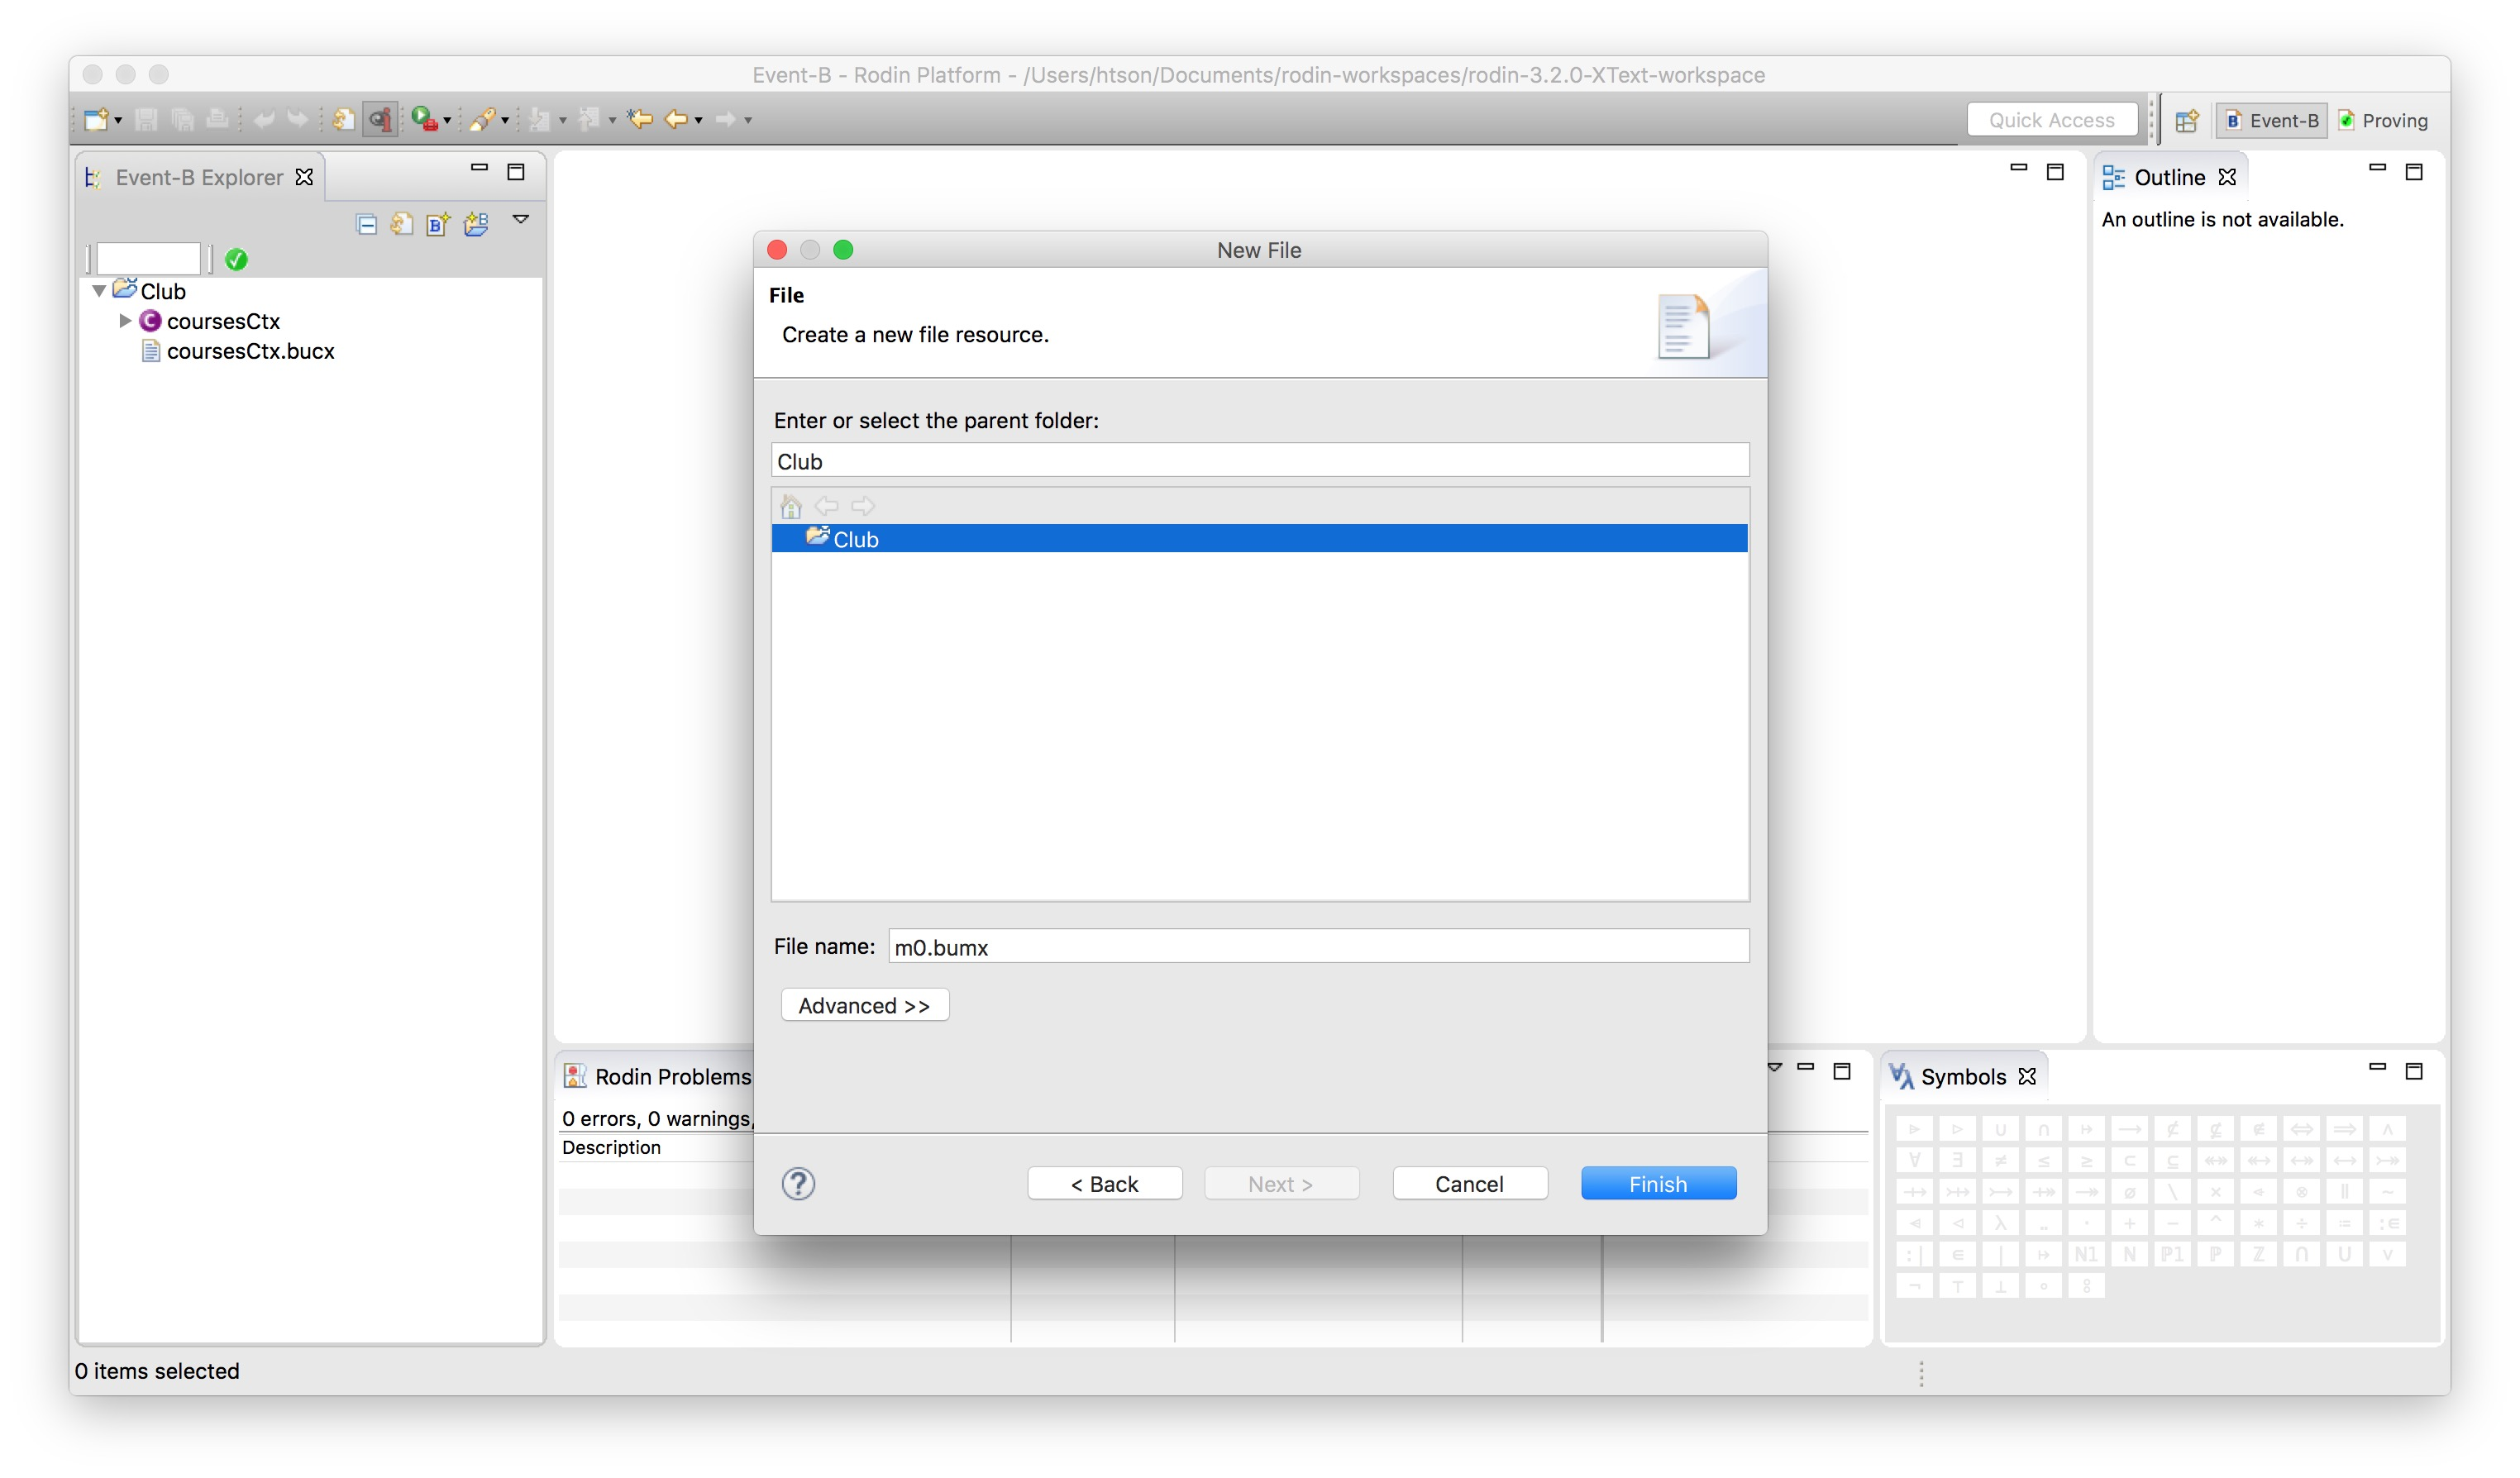
\includegraphics[width=512]{figures/CreateM0}
    \else
    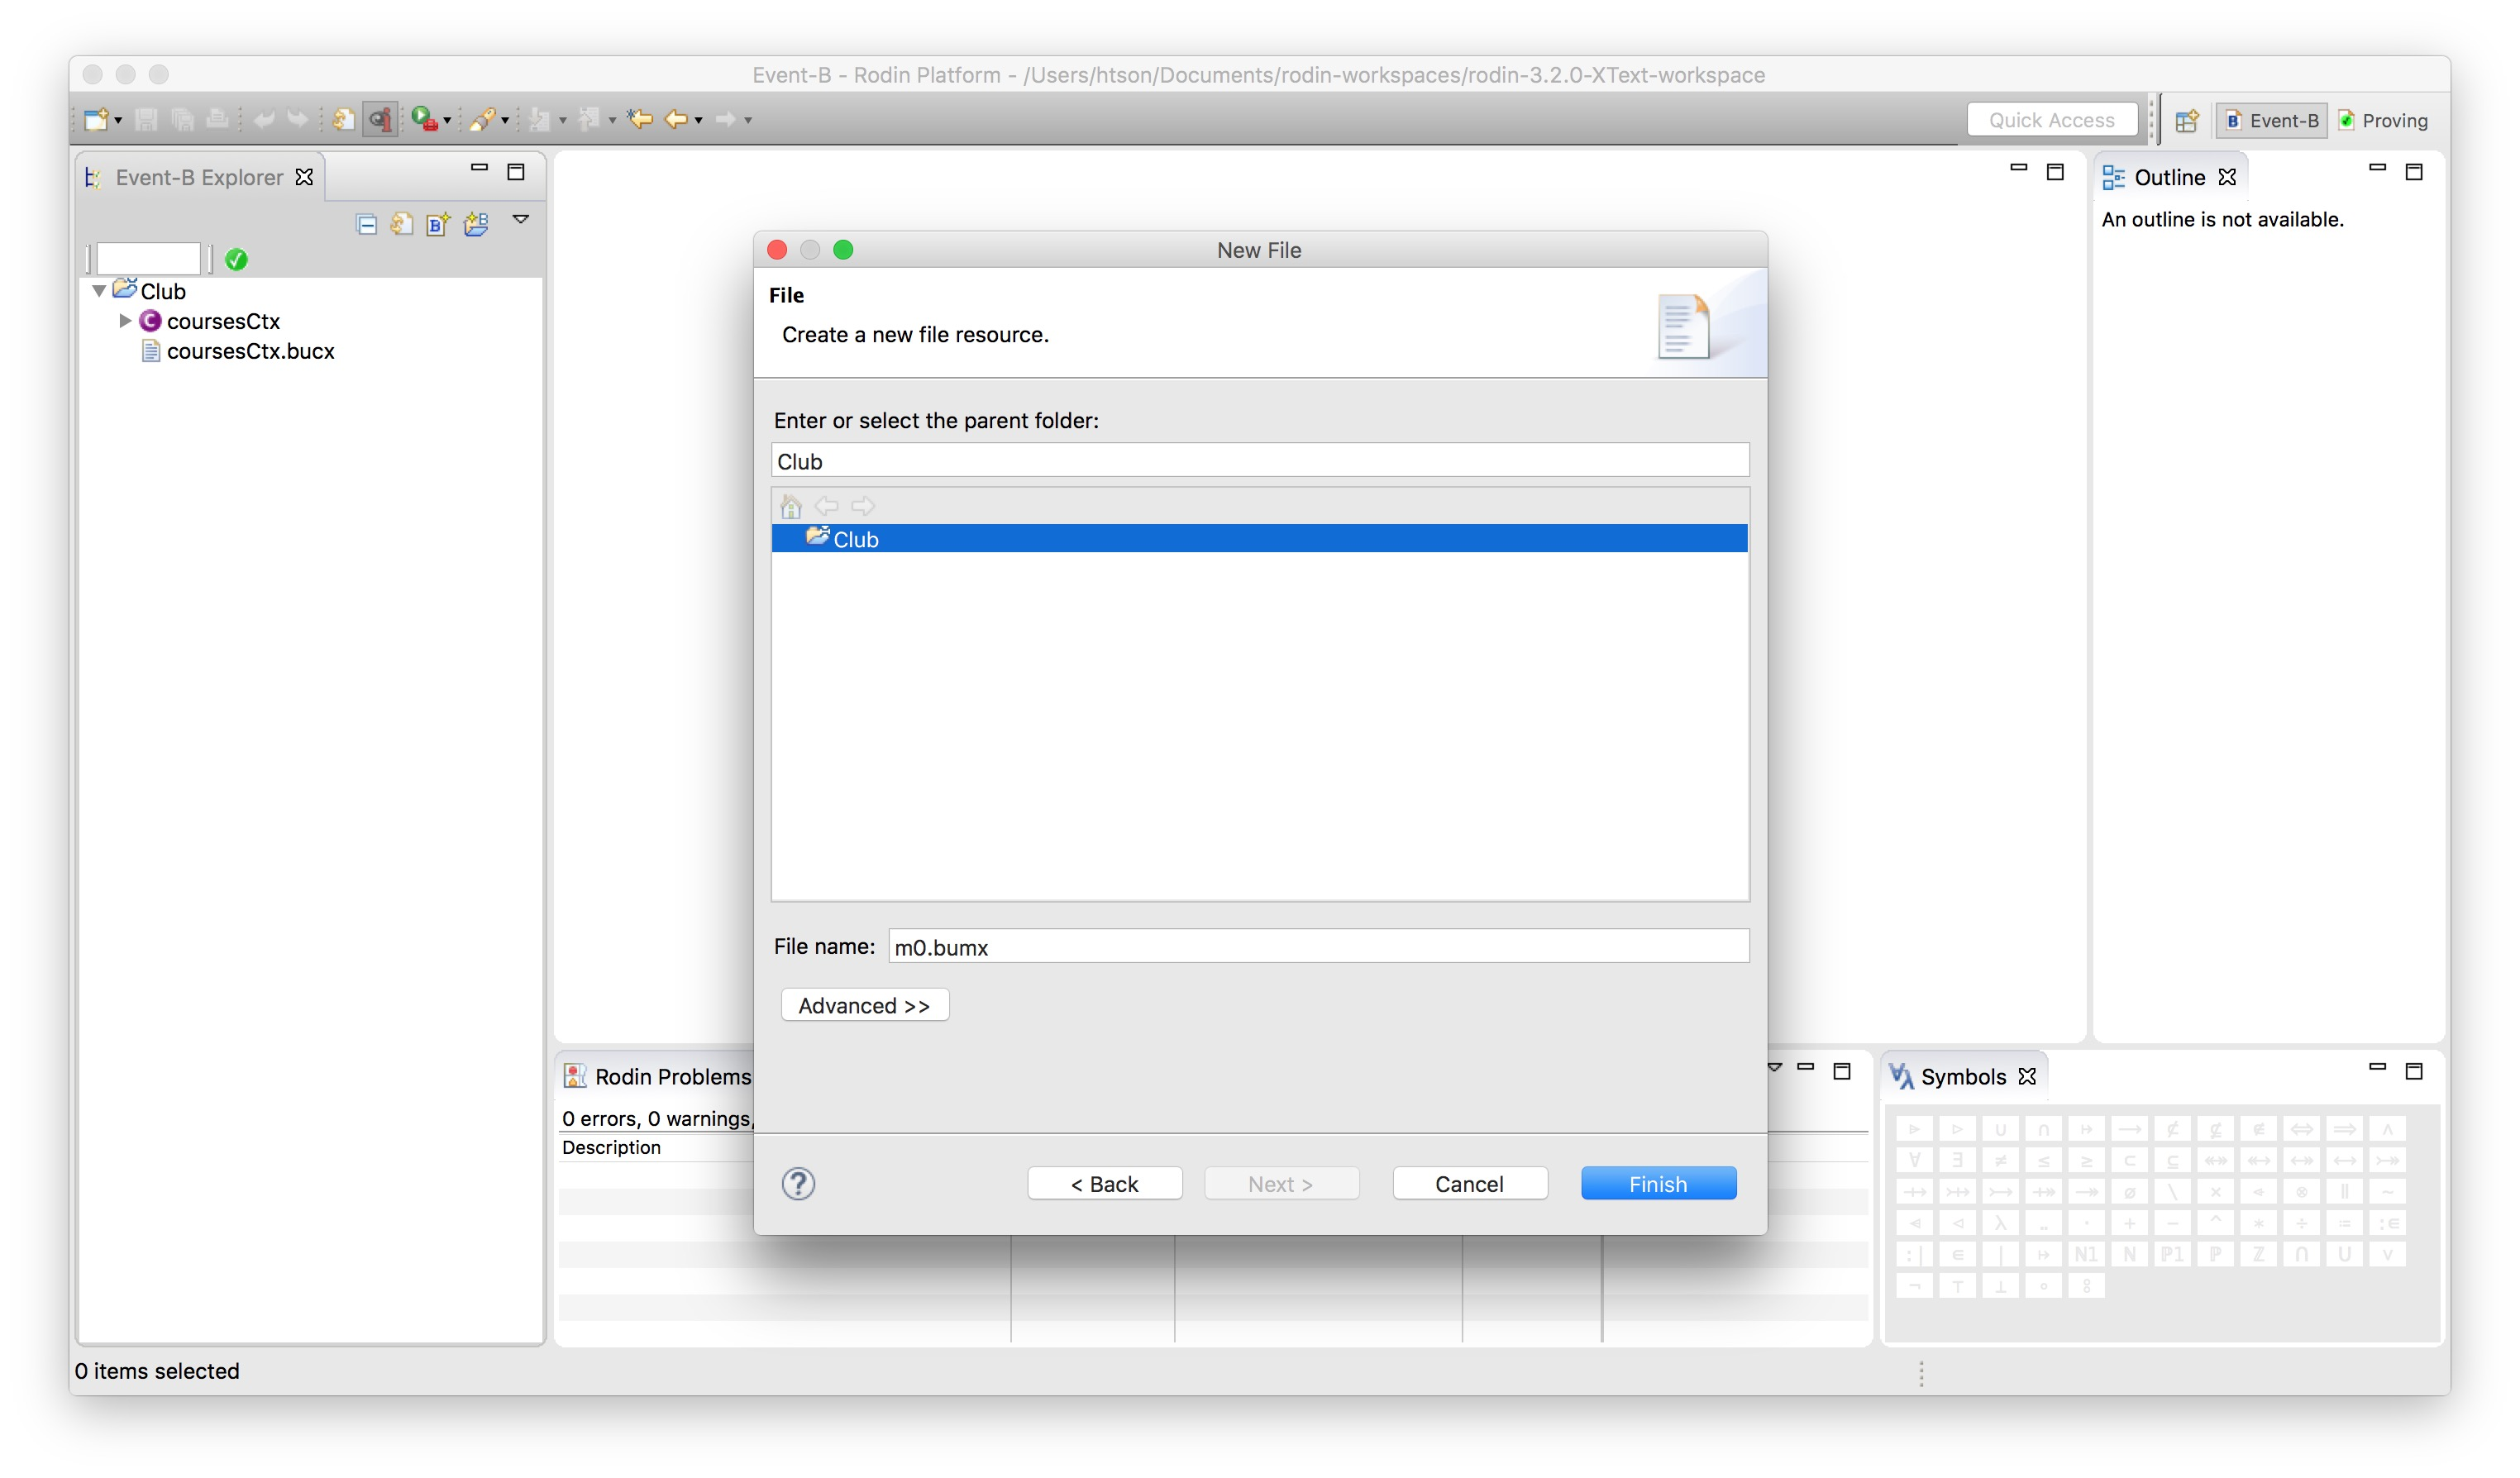
\includegraphics[width=0.9\textwidth]{figures/CreateM0}
    \endif
    \caption{Type-setting \ifdef{PLASTEX} ℕ1 \else $\natn$ \endif using Content Assist}
    \label{fig:CreateM0}
  \end{figure}

\item[Step 2. Set the content of m0.bumx] \textbf{Set the content of "m0.bumx" as follows}.
  \begin{center}
    \begin{Bcode}
      \ifdef{PLASTEX}
      \Bmachine{} m0 \\
      \Bvariables{} crs \\
      \Binvariants \\
      @inv0_1: crs ∈ ℙ(CRS)\\
      \Btheorem{} @thm0_2: finite(crs) \\
      @inv0_2: card(crs) ≤ m \\
      @DLF: (card(crs) ≠ m) ∨ (∃cs·cs ⊆ crs ∧ cs ≠ ∅) \\
      \Bevents\\
      event INITIALISATION\\
      \Bthen \\
      @act0_1: crs ≔ ∅\\
      \Bend\\
      event OpenCourses\\
      \Bwhere\\
      @grd0_1: card(crs) ≠ m\\
      \Btheorem{} @thm0_3: crs ≠ CRS\\
      \Bthen\\
      @act0_1: crs :∣ crs ⊂ crs' ∧ card(crs') ≤ m\\
      \Bend\\
      \Banticipated{} event CloseCourses \\
      \Bany{} cs \Bwhere\\
      @grd0_1: cs ⊆ crs\\
      @grd0_2: cs ≠ ∅\\
      \Bthen\\
      @act0_1: crs ≔ crs ∖ cs\\
      \Bend\\
      \Bend
      \else
      \Bmachine{} m0 \\
      \Bvariables{} crs \\
      \Binvariants \\
      \Btab @inv0\_1: \(crs \in \pow(CRS)\)\\
      \Btab \Btheorem{} @thm0\_2: \(\finite(crs)\) \\
      \Btab @inv0\_2: \(\card(crs) \leq m\) \\
      \Btab @DLF: \((\card(crs) \neq m) \lor (\exists cs \qdot cs \subseteq crs \land cs \neq \emptyset)\) \\
      \Bevents\\
      \Btab event INITIALISATION\\
      \Btab \Bbegin \\
      \Btab\Btab @act0\_1: \(crs \bcmeq \emptyset\)\\
      \Btab \Bend\\
      \Btab event OpenCourses\\
      \Btab \Bwhere\\
      \Btab \Btab @grd0\_1: \(\card(crs) \neq m\) \\
      \Btab \Btab \Btheorem{} @thm0\_3: \(crs \neq CRS\) \\
      \Btab \Bthen\\
      \Btab \Btab @act0\_1: \(crs \bcmsuch crs \subset crs' \land \card(crs') \leq m\)\\
      \Btab \Bend\\
      \Btab \Banticipated{} event CloseCourses \\
      \Btab \Bany{} cs \Bwhere\\
      \Btab \Btab @grd0\_1: \(cs \subseteq crs\)\\
      \Btab \Btab @grd0\_2: \(cs \neq \emptyset\)\\
      \Btab \Bthen\\
      \Btab \Btab @act0\_1: \(crs \bcmeq crs \setminus cs\)\\
      \Btab \Bend\\
      \Bend
      \endif
    \end{Bcode}
  \end{center}
\item[Step 3. Auto-format the code] \textbf{Automatically format the content of ``m0.bumx''} by using short-cut (e.g., on Mac OS: Cmd+Shift+F).

\item[Step 4. Save the file] \textbf{Save the file ``m0.bumx''}.

\item[Step 5. Add missing ``sees'' clause] In the compiled Rodin Machine m0, there are several errors, due to the fact that \textbf{m0} refers to the sets and constants of the context courseCtx.
  \textbf{Add the missing ``sees'' clause} after the ``machine'' clause
  \begin{center}
    \begin{Bcode}
      \Bsees{} courseCtx
    \end{Bcode}
  \end{center}
  (Note: One can use \emph{Content Assist} after typing the ``sees'' keyword to select the context, see Figure~\ref{fig:SeesCoursesCtx}).
  \begin{figure}[!htbp]
    \centering
    \ifdef{PLASTEX}
    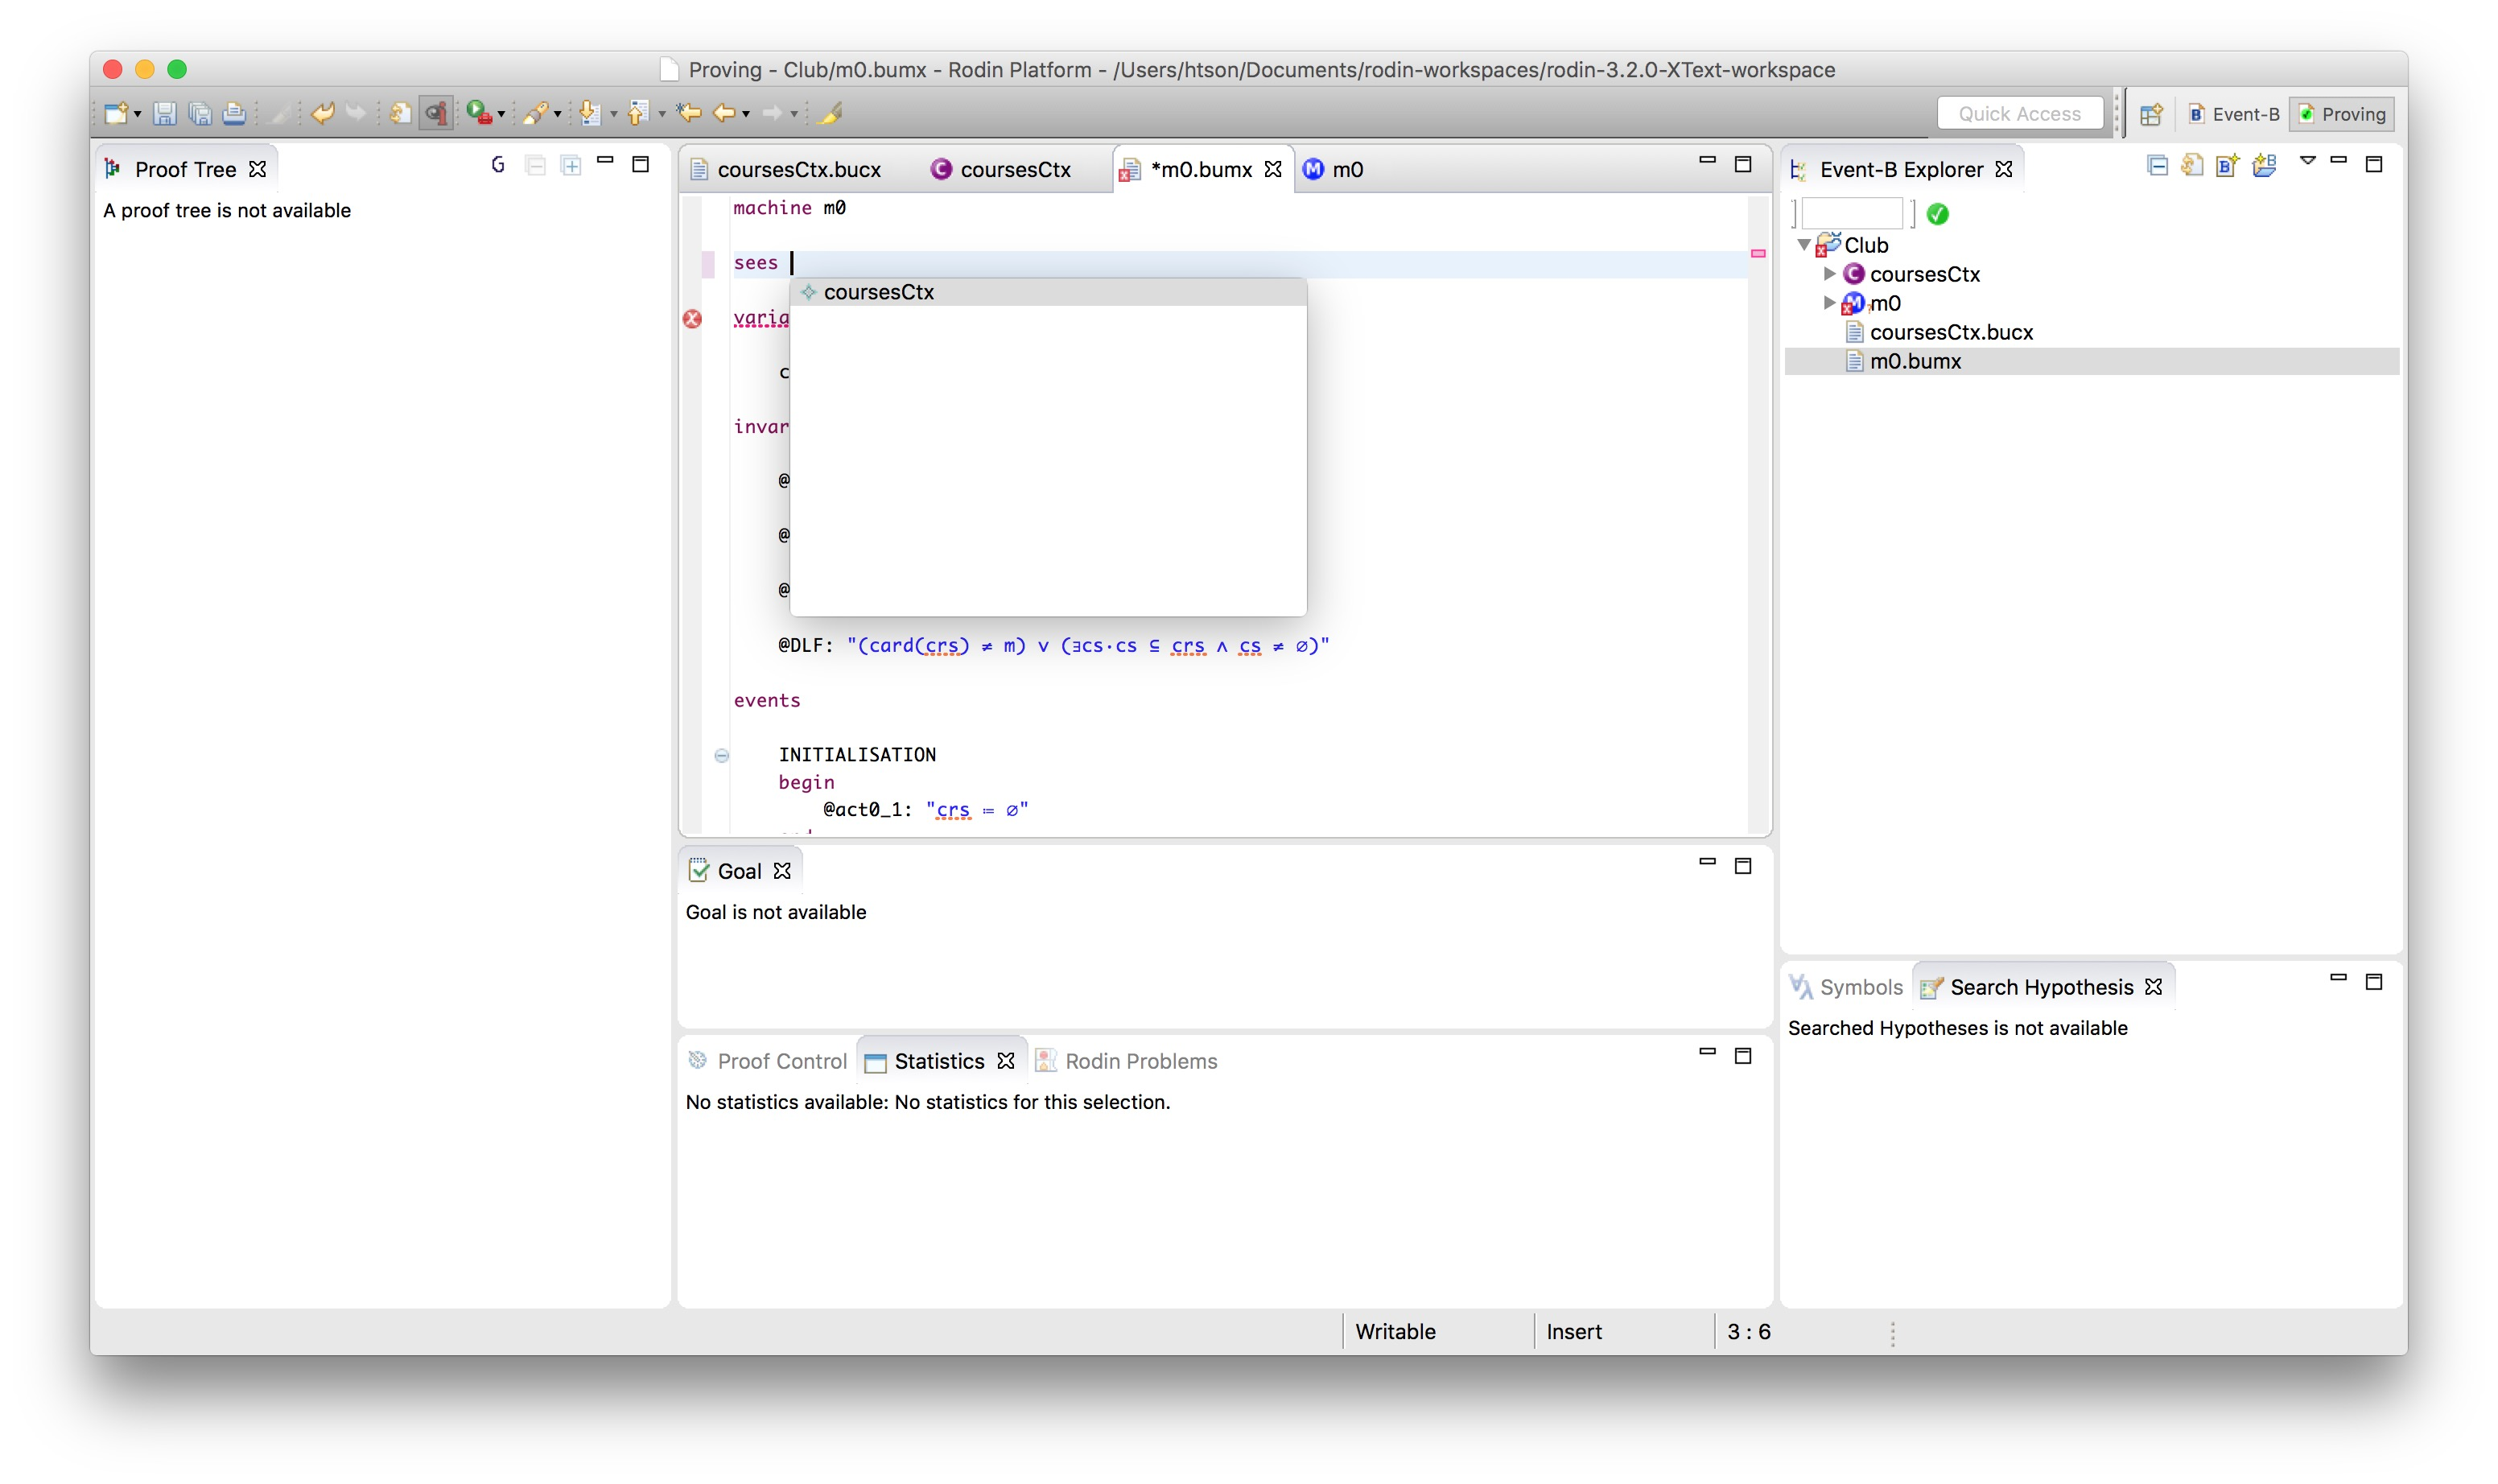
\includegraphics[width=512]{figures/SeesCoursesCtx}
    \else
    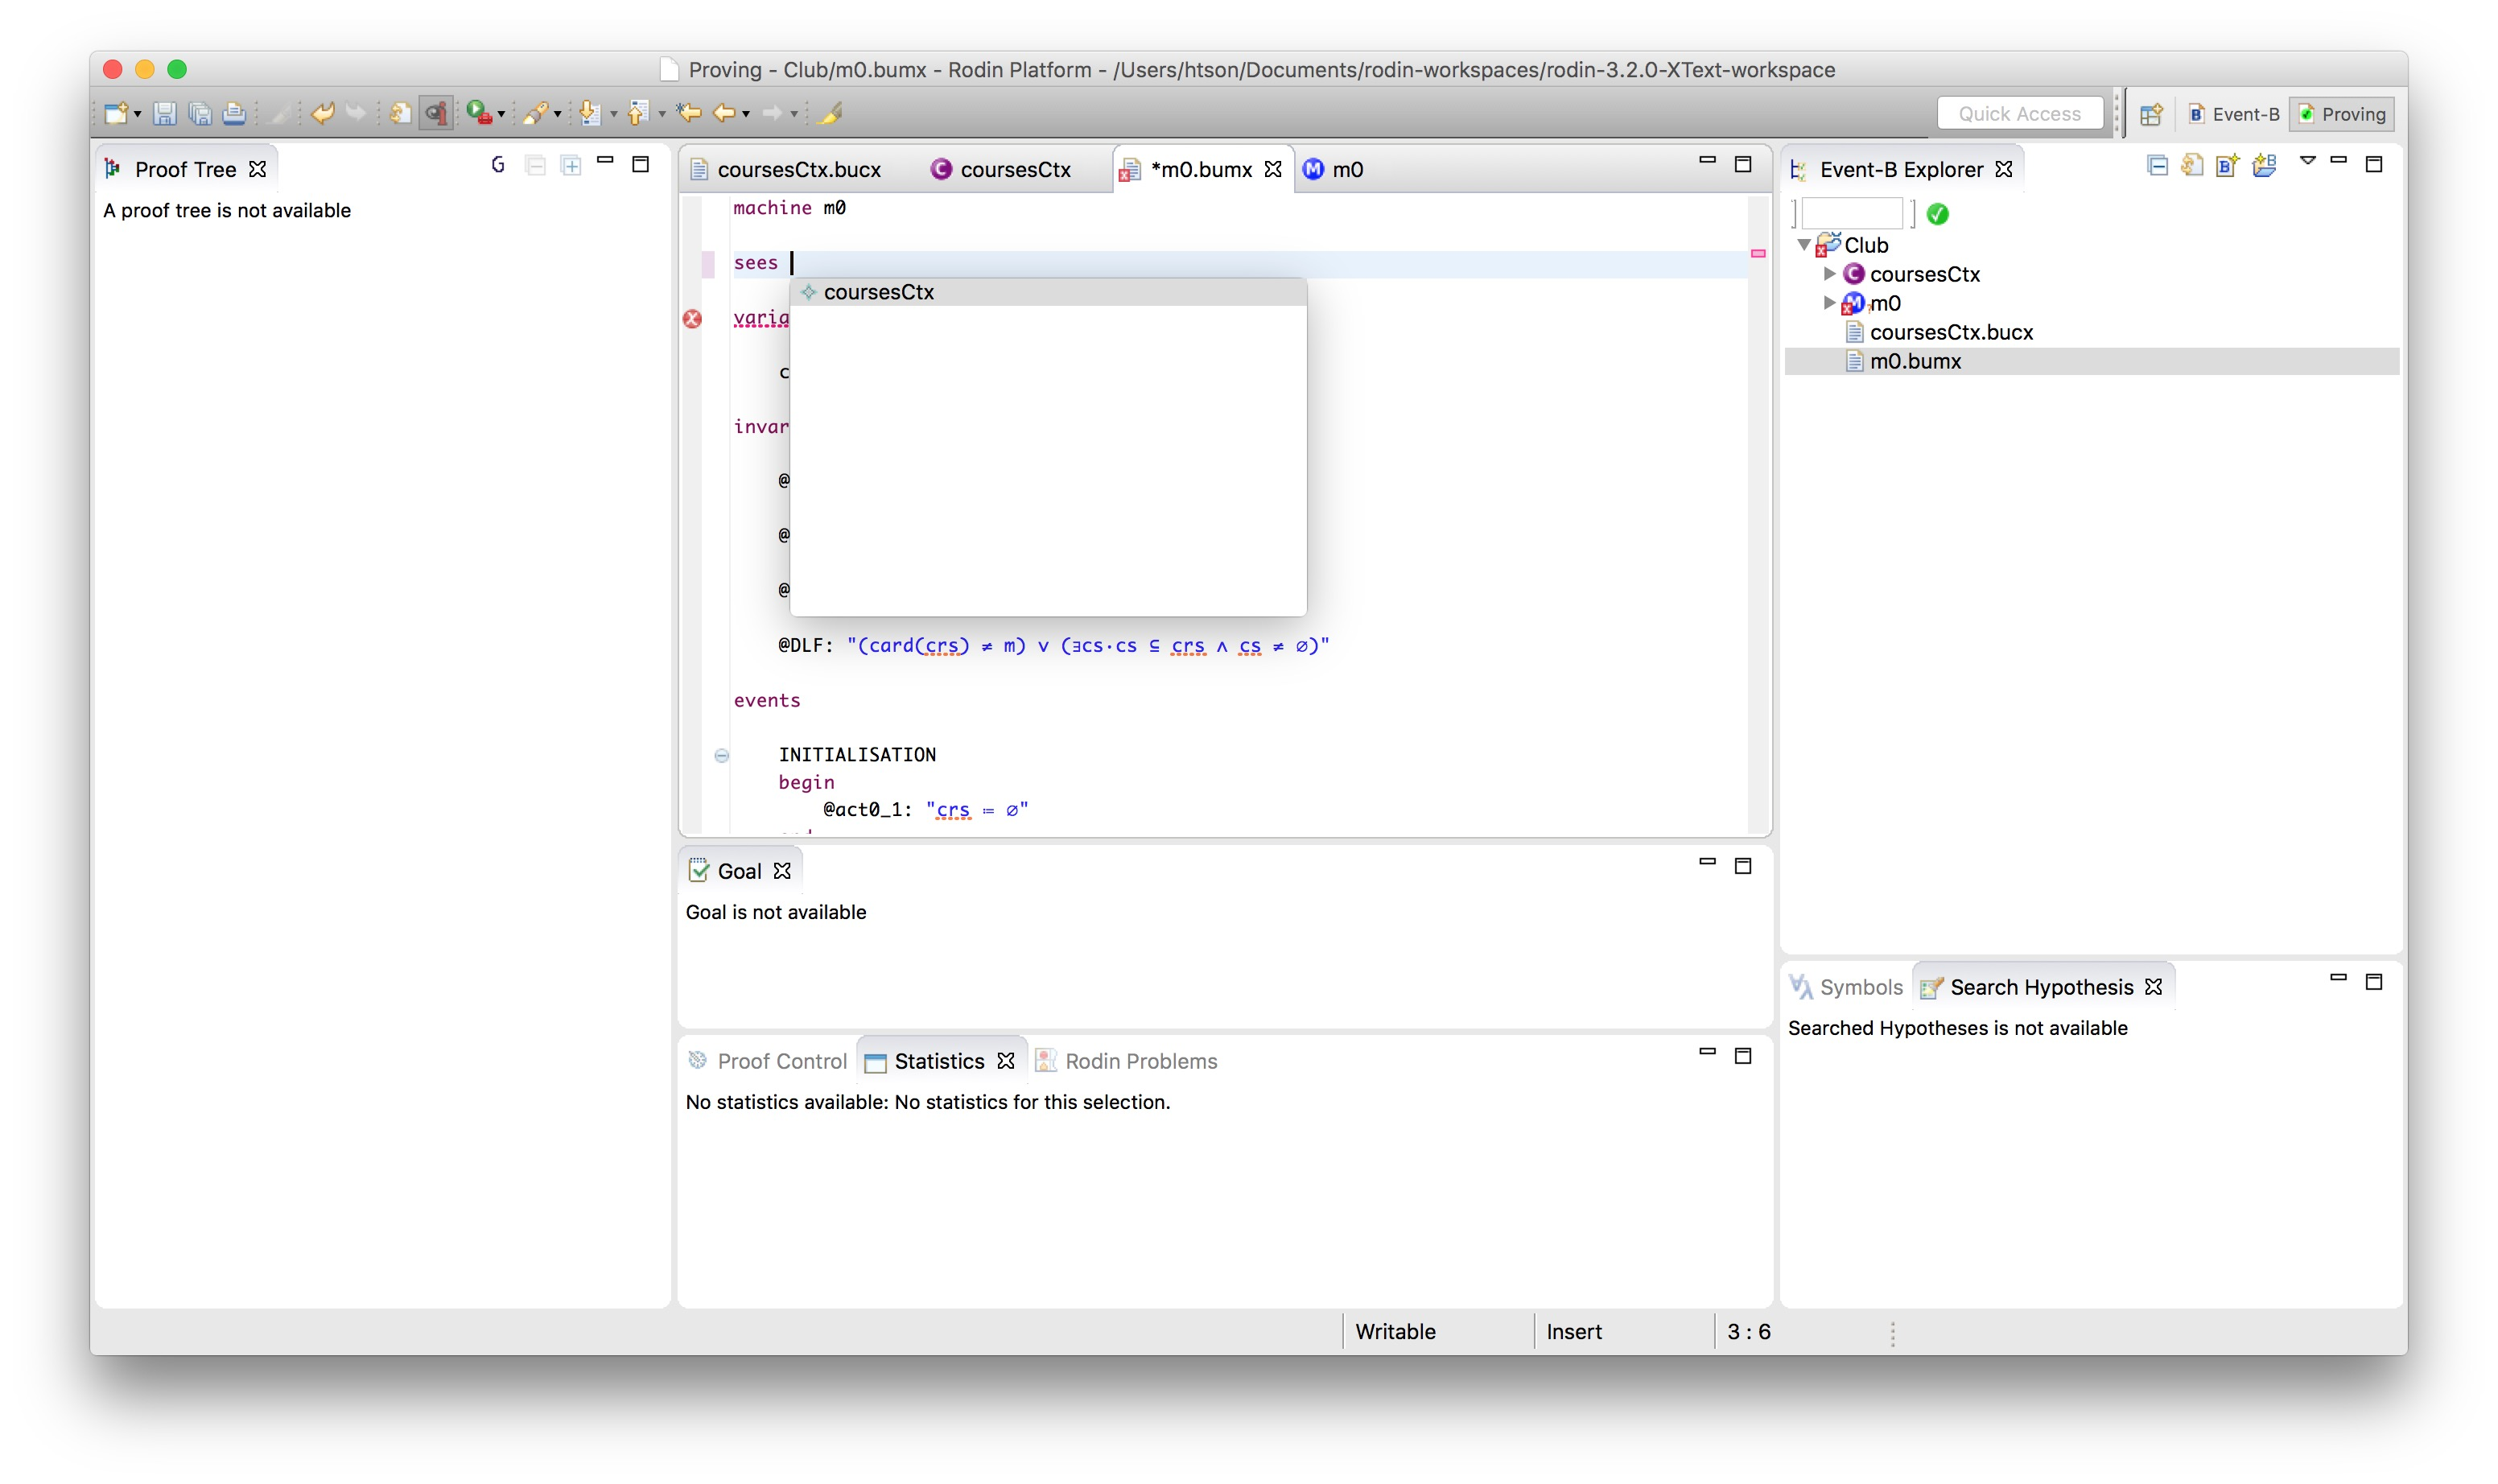
\includegraphics[width=0.9\textwidth]{figures/SeesCoursesCtx}
    \endif
    \caption{Content Assist for adding Sees clause}
    \label{fig:SeesCoursesCtx}
  \end{figure}

\item[Step 6. Save the file again] \textbf{Save the file "m0.bumx" again}.
\end{description}
\textbf{Conclusion} By now, the XMachine ``m0.bumx'' and the corresponding Rodin Machine ``m0'' (without any error) should be visible in the Event-B Explorer (see Figure~\ref{fig:M0}.
  \begin{figure}[!htbp]
    \centering
    \ifdef{PLASTEX}
    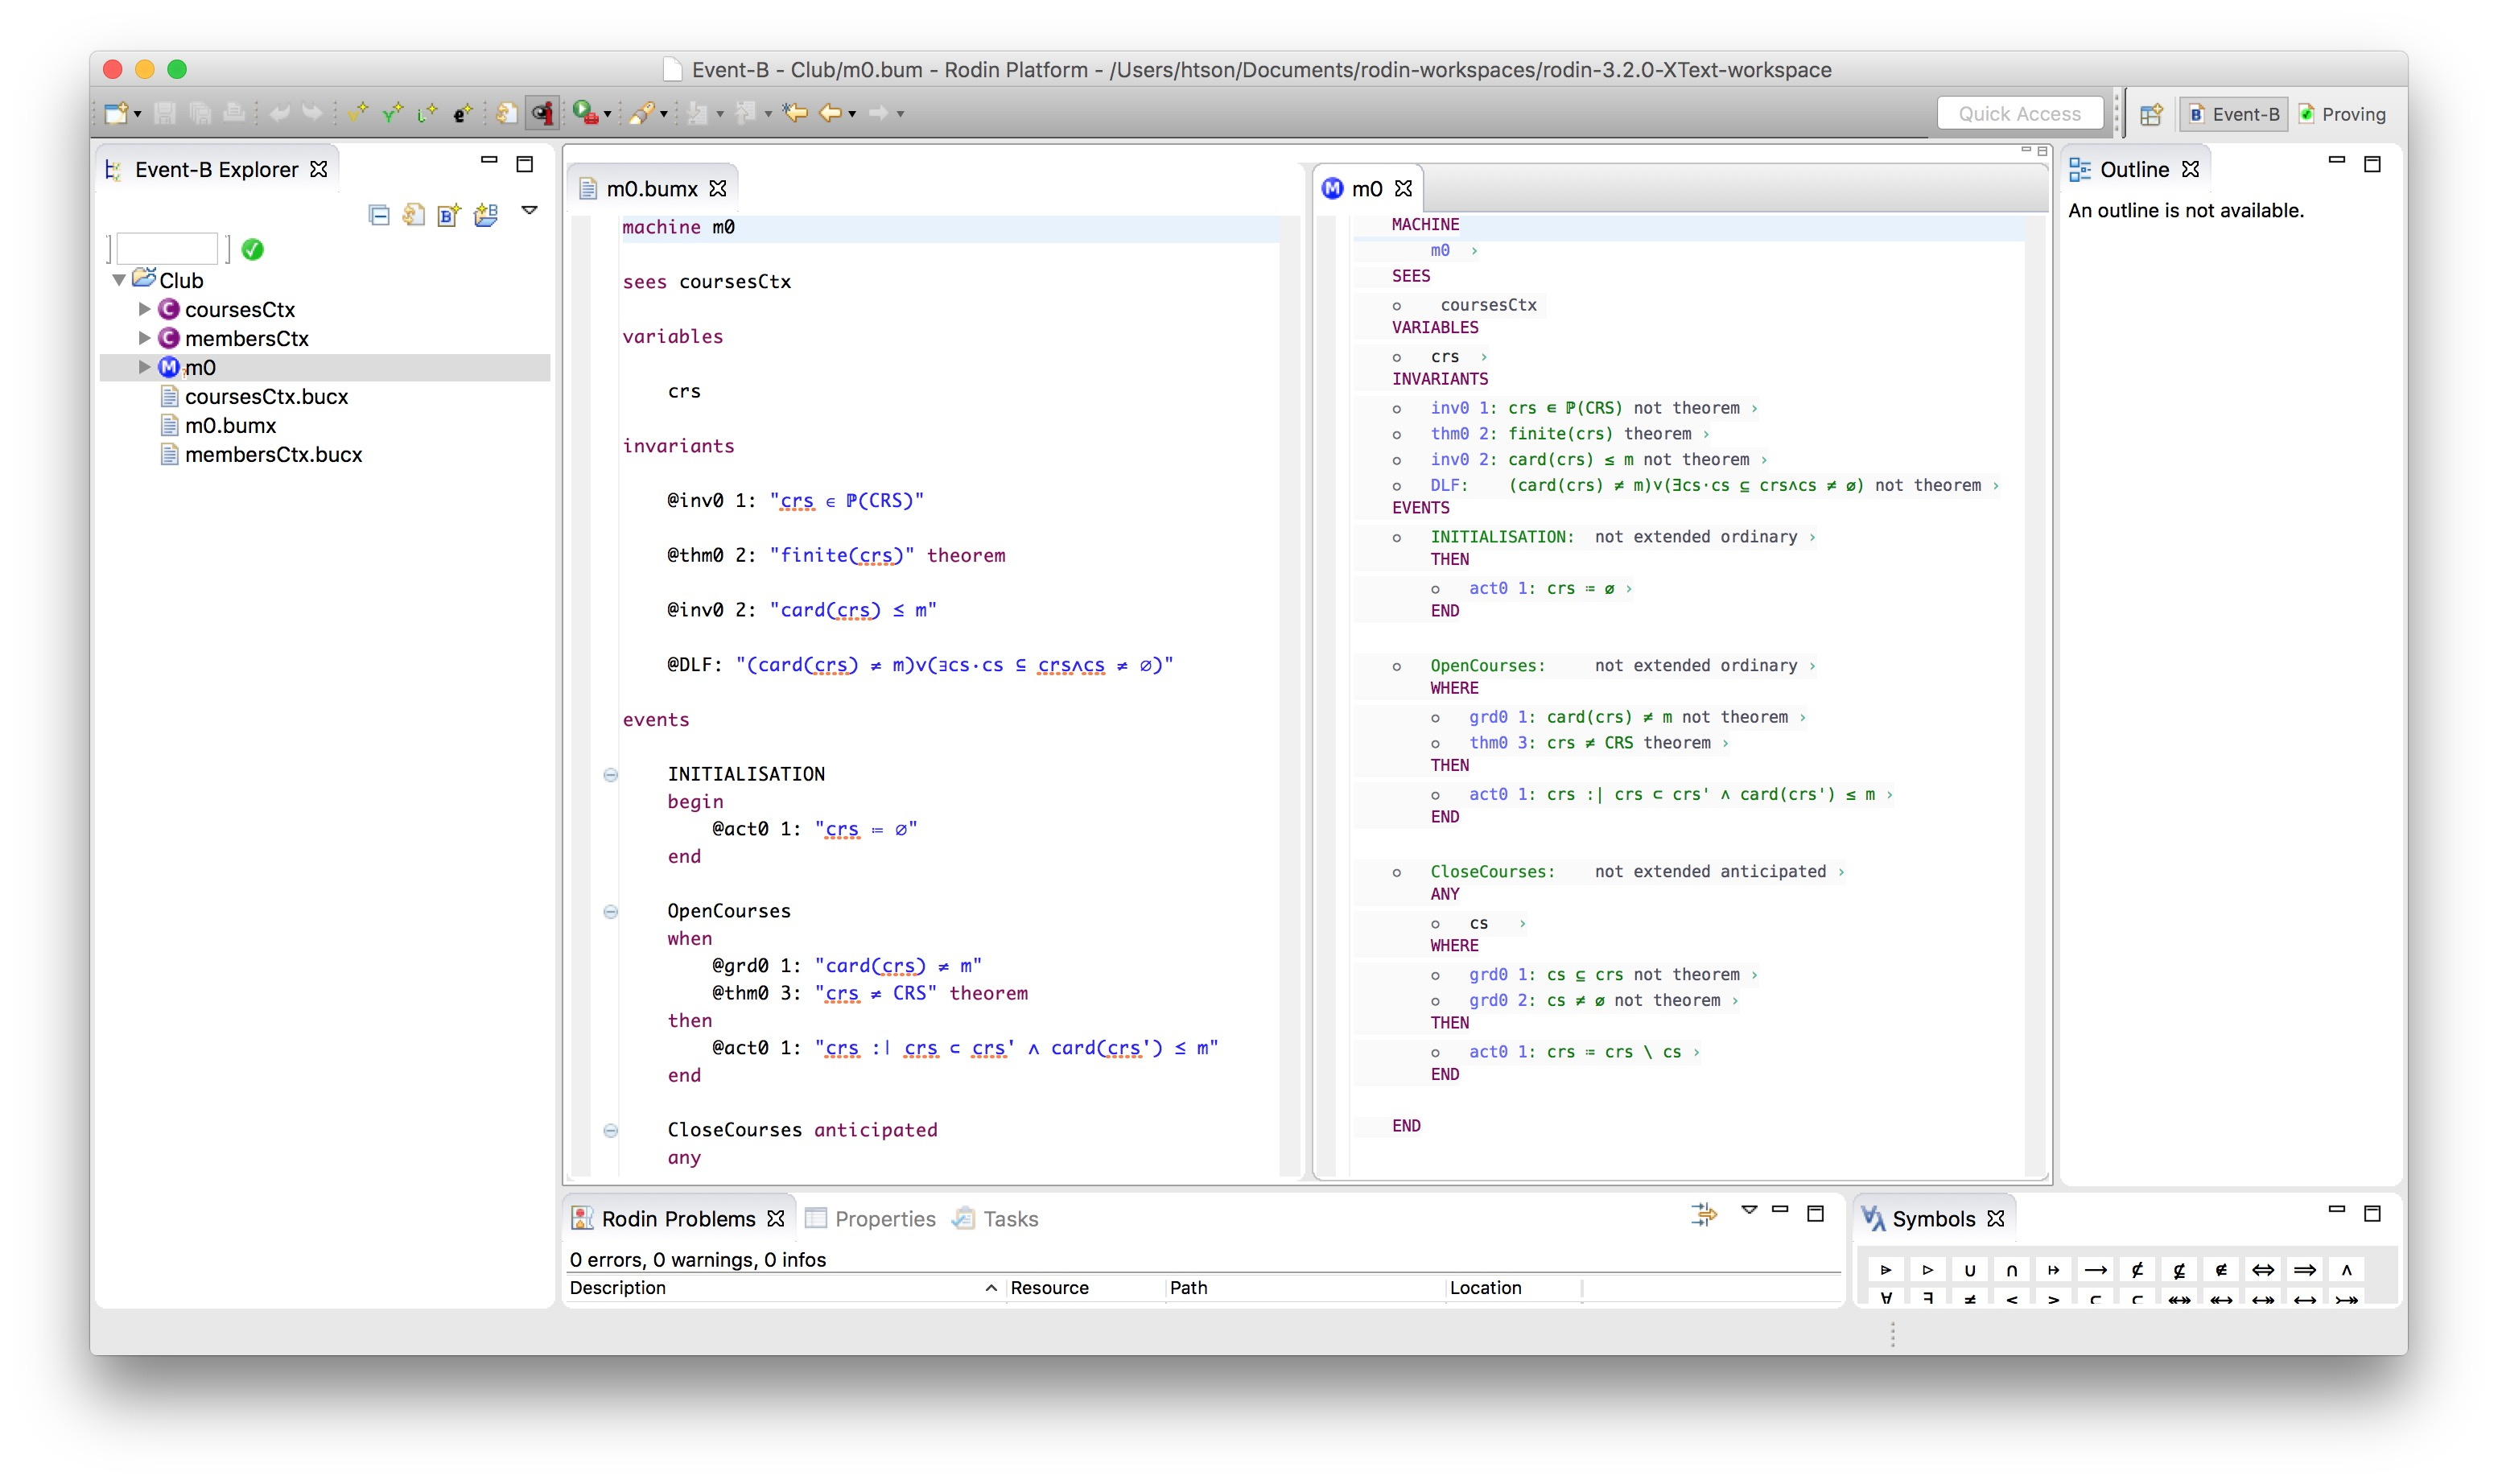
\includegraphics[width=512]{figures/M0}
    \else
    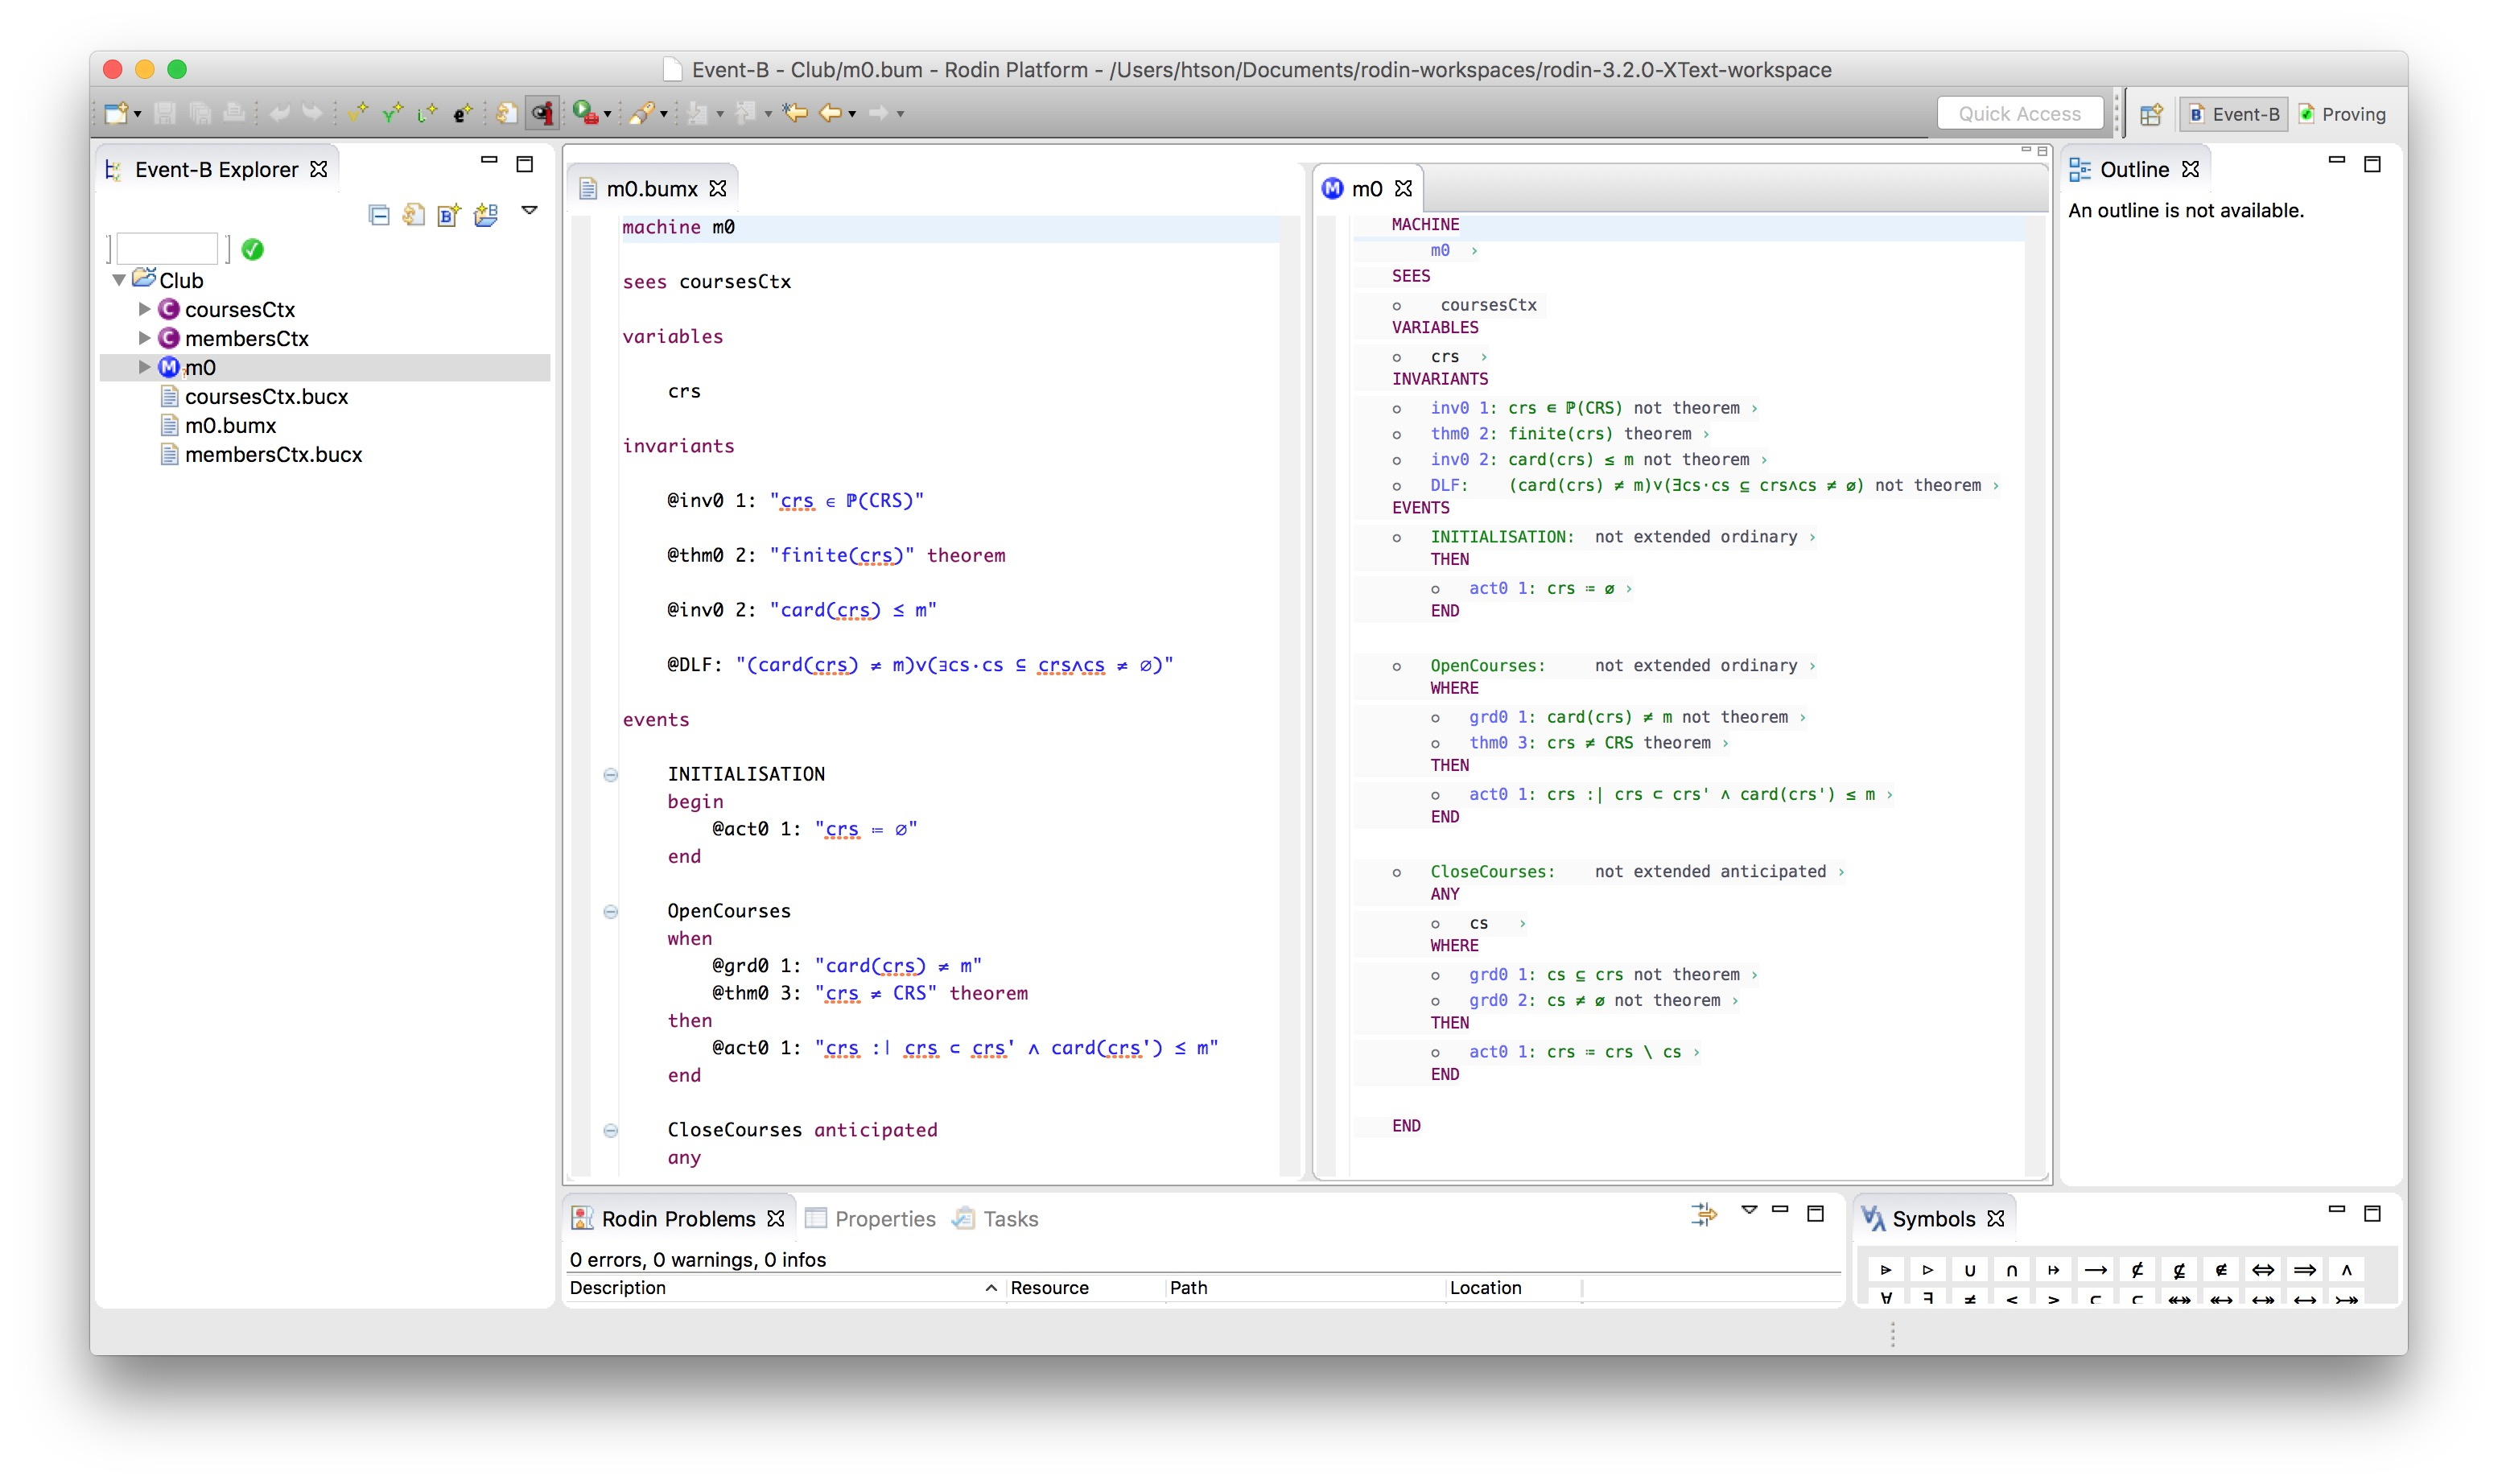
\includegraphics[width=0.9\textwidth]{figures/M0}
    \endif
    \caption{XMachine m0.bucx}
    \label{fig:M0}
  \end{figure}

\subsubsection{Task 5. Create extended XContexts}
\textbf{Introduction} The purpose of this task is to create some more extended XContexts within the "Club" project.

\paragraph{Task 5.1. Create a simple XContext membersCtx.bucx}
\textbf{Introduction} The purpose of this sub-task is to create a simple XContext ``membersCtx.bucx'' within the ``Club'' project.
\begin{description}
\item[Step 1. Create a new XContext membersCtx.bucx] \textbf{Create a new XContext} named ``membersCtx.bucx'' using the \emph{New File} wizard (see Figure~\ref{fig:CreateMembersCtx}.
  \begin{figure}[!htbp]
    \centering
    \ifdef{PLASTEX}
    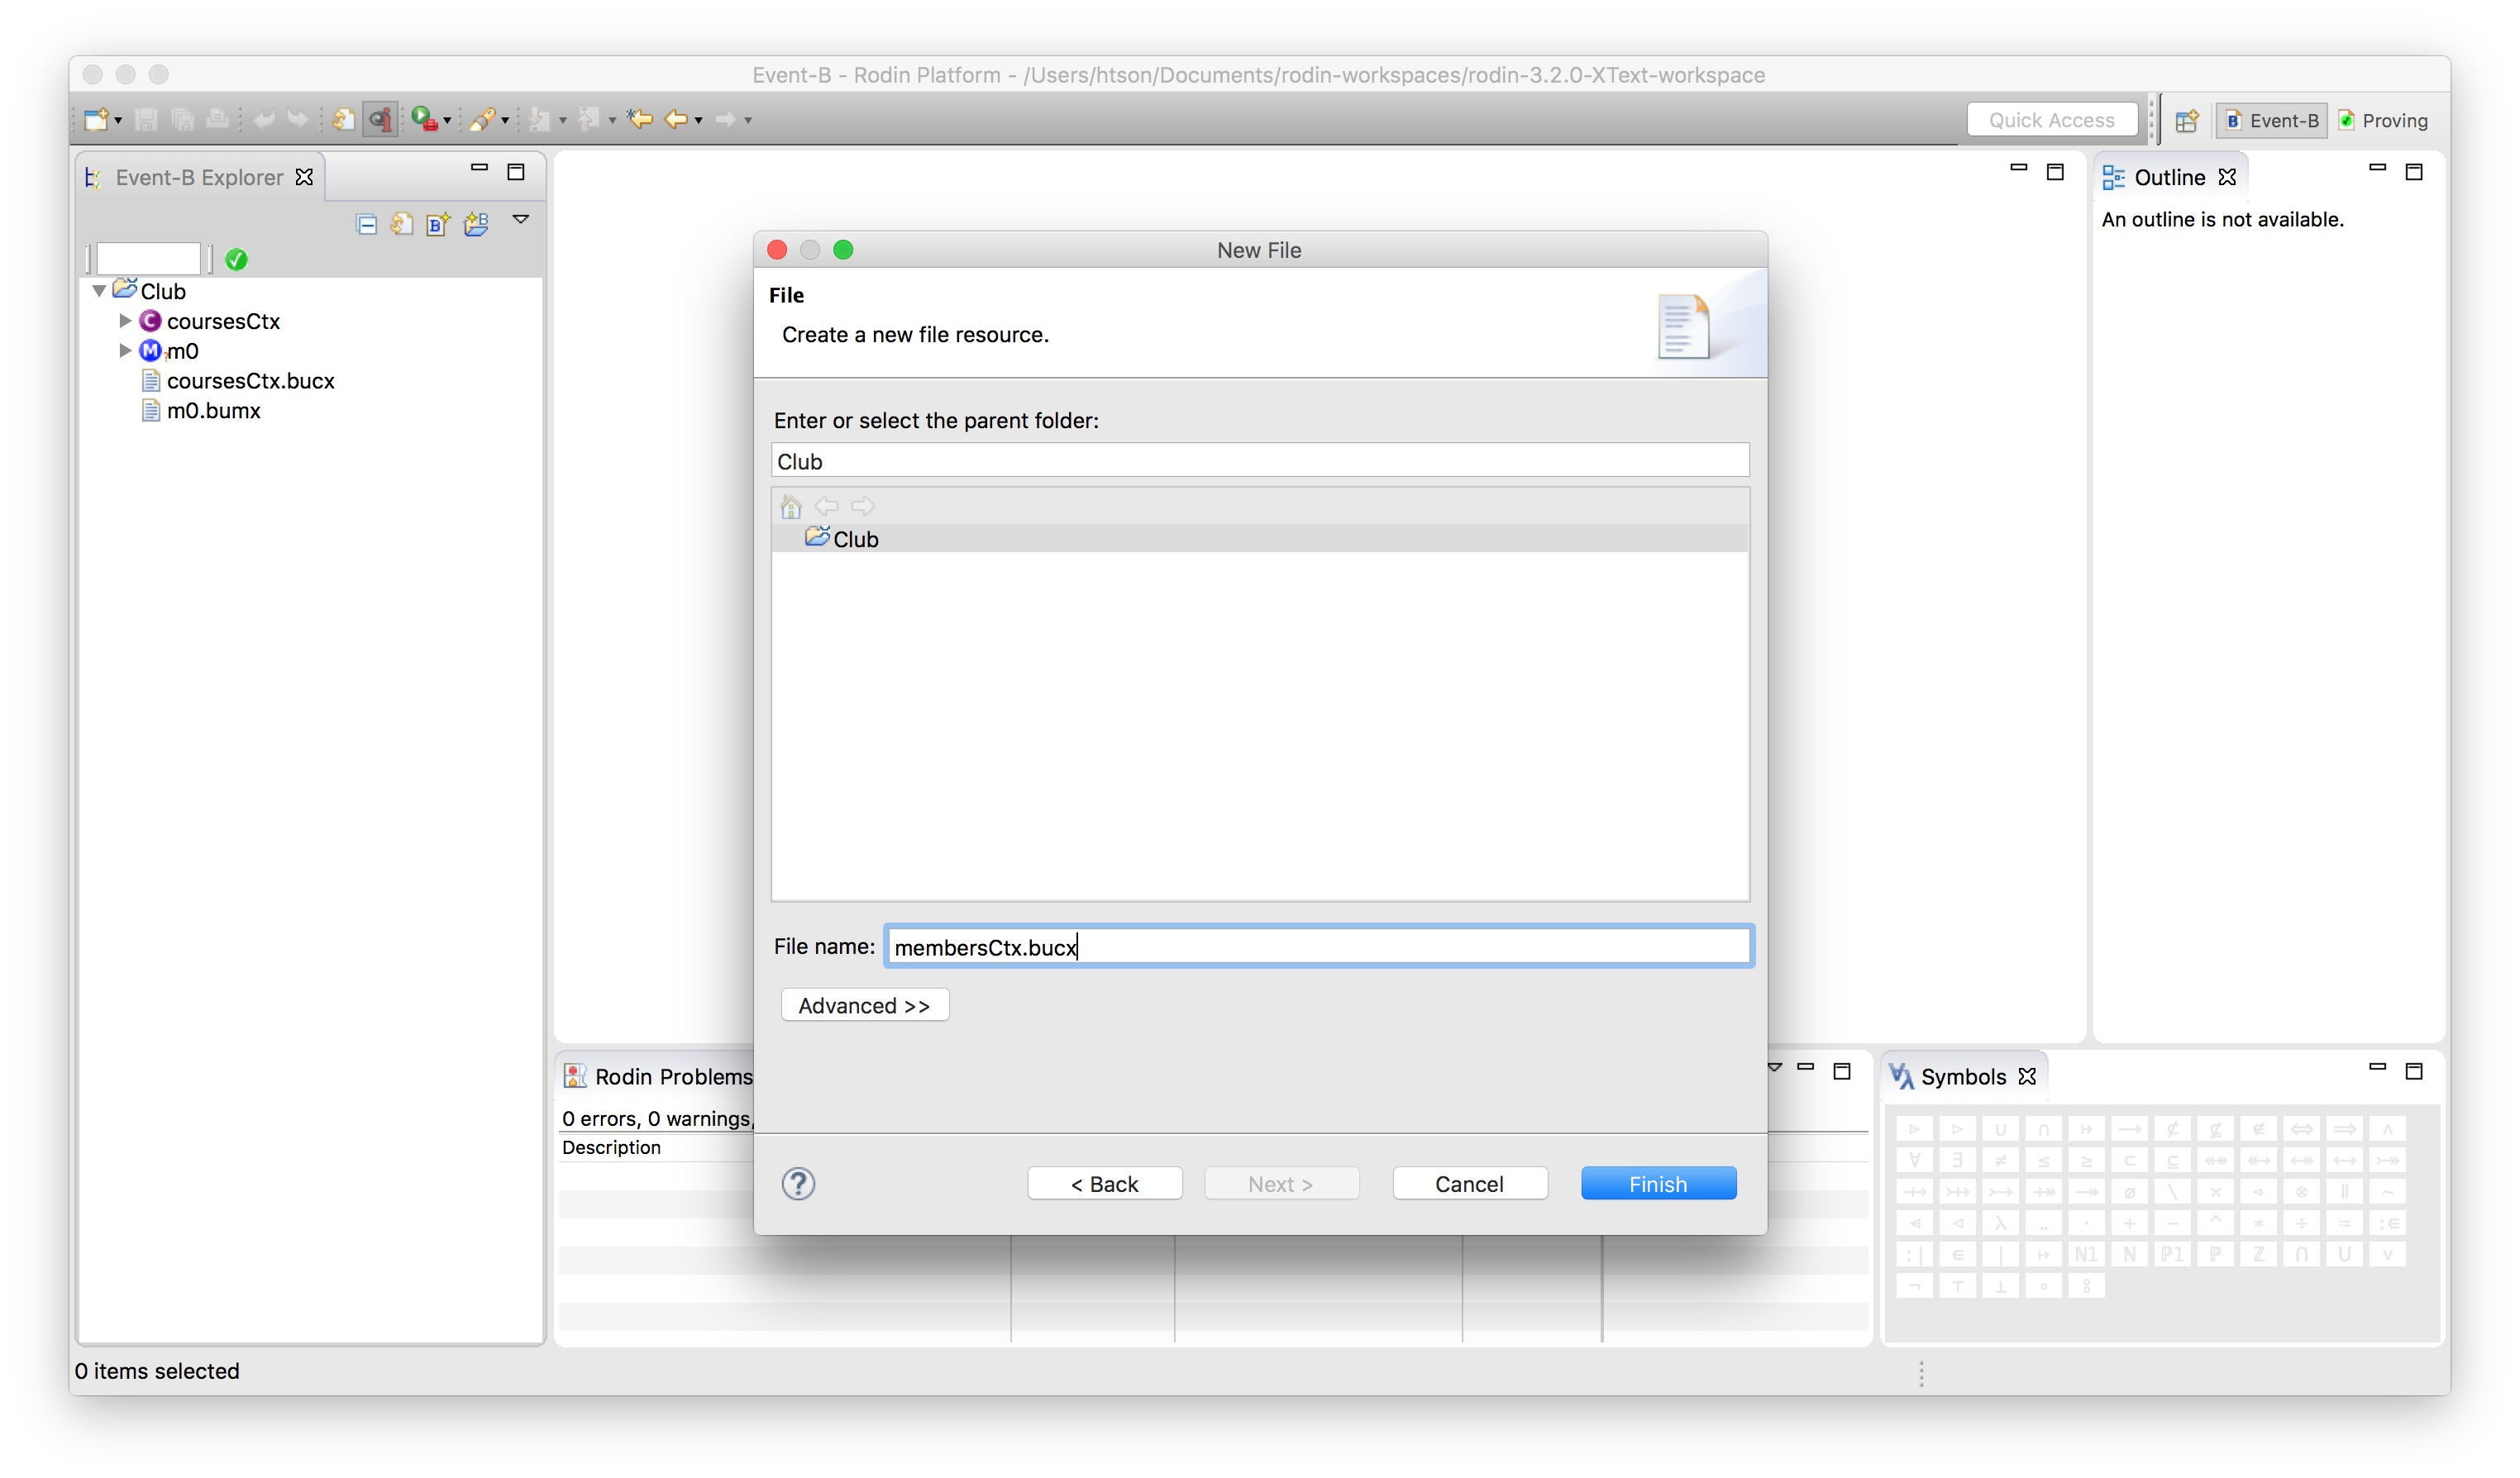
\includegraphics[width=512]{figures/CreateMembersCtx}
    \else
    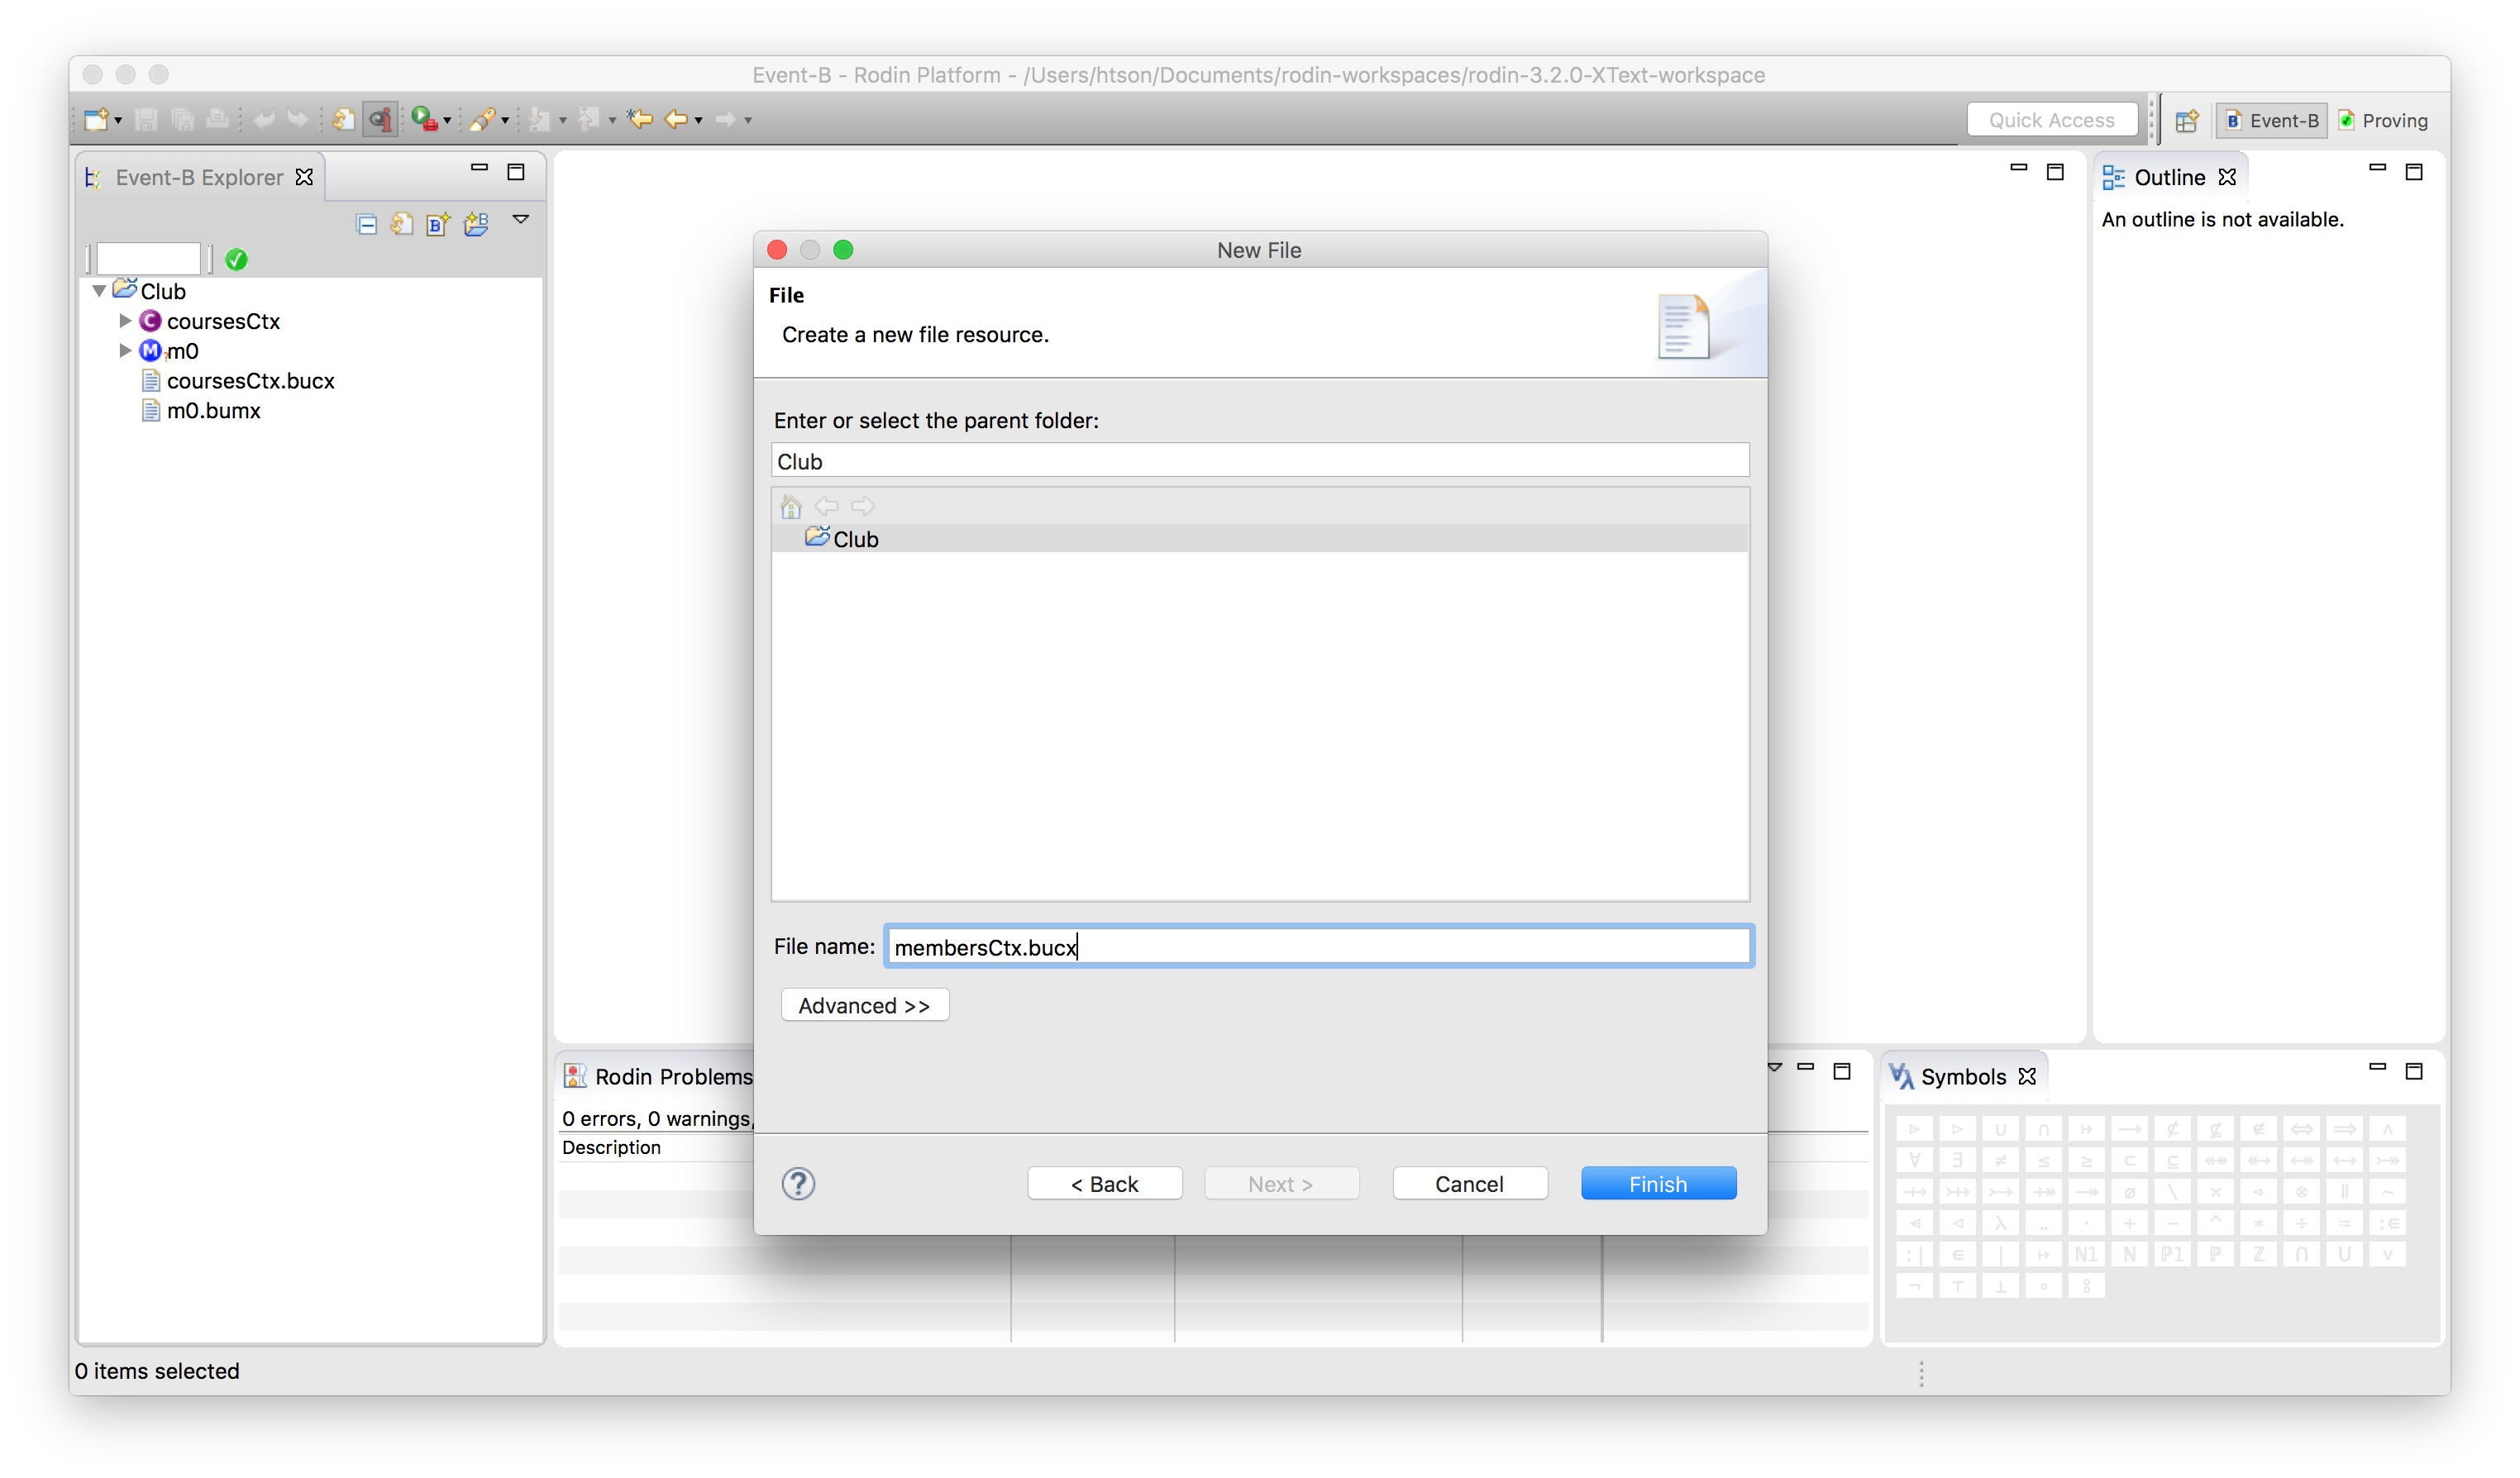
\includegraphics[width=0.9\textwidth]{figures/CreateMembersCtx}
    \endif
    \caption{Create membersCtx.bucx}
    \label{fig:CreateMembersCtx}
  \end{figure}

\item[Step 2. Set the content of membersCtx.bucx] \textbf{Set the content of ``membersCtx.bucx'' as follows}.
  \begin{center}
    \begin{Bcode}
      \ifdef{PLASTEX}
      \Bcontext{} memebersCtx\\
      \Bsets{} MEM\\
      \Baxioms\\
      @axm0_1: finite(MEM)\\
      \Bend
      \else
      \Bcontext{} memebersCtx\\
      \Bsets{} MEM\\
      \Baxioms\\
      \Btab @axm0_1: \(\finite(MEM)\)\\
      \Bend
      \endif
    \end{Bcode}
  \end{center}

\item [Step 3. Auto-format the code] \textbf{Automatically format the content of ``membersCtx.bucx''} by using short-cut (e.g., on Mac OS: Cmd+Shift+F).

\item[Step 4. Save the file] Save the file \textbf{``membersCtx.bucx''}.
\end{description}

\textbf{Conclusion} By now, the XContext ``membersCtx.bucx'' and the corresponding Rodin Context ``membersCtx'' should be visible in the Event-B Explorer (see Figure~\ref{fig:membersCtx}.
  \begin{figure}[!htbp]
    \centering
    \ifdef{PLASTEX}
    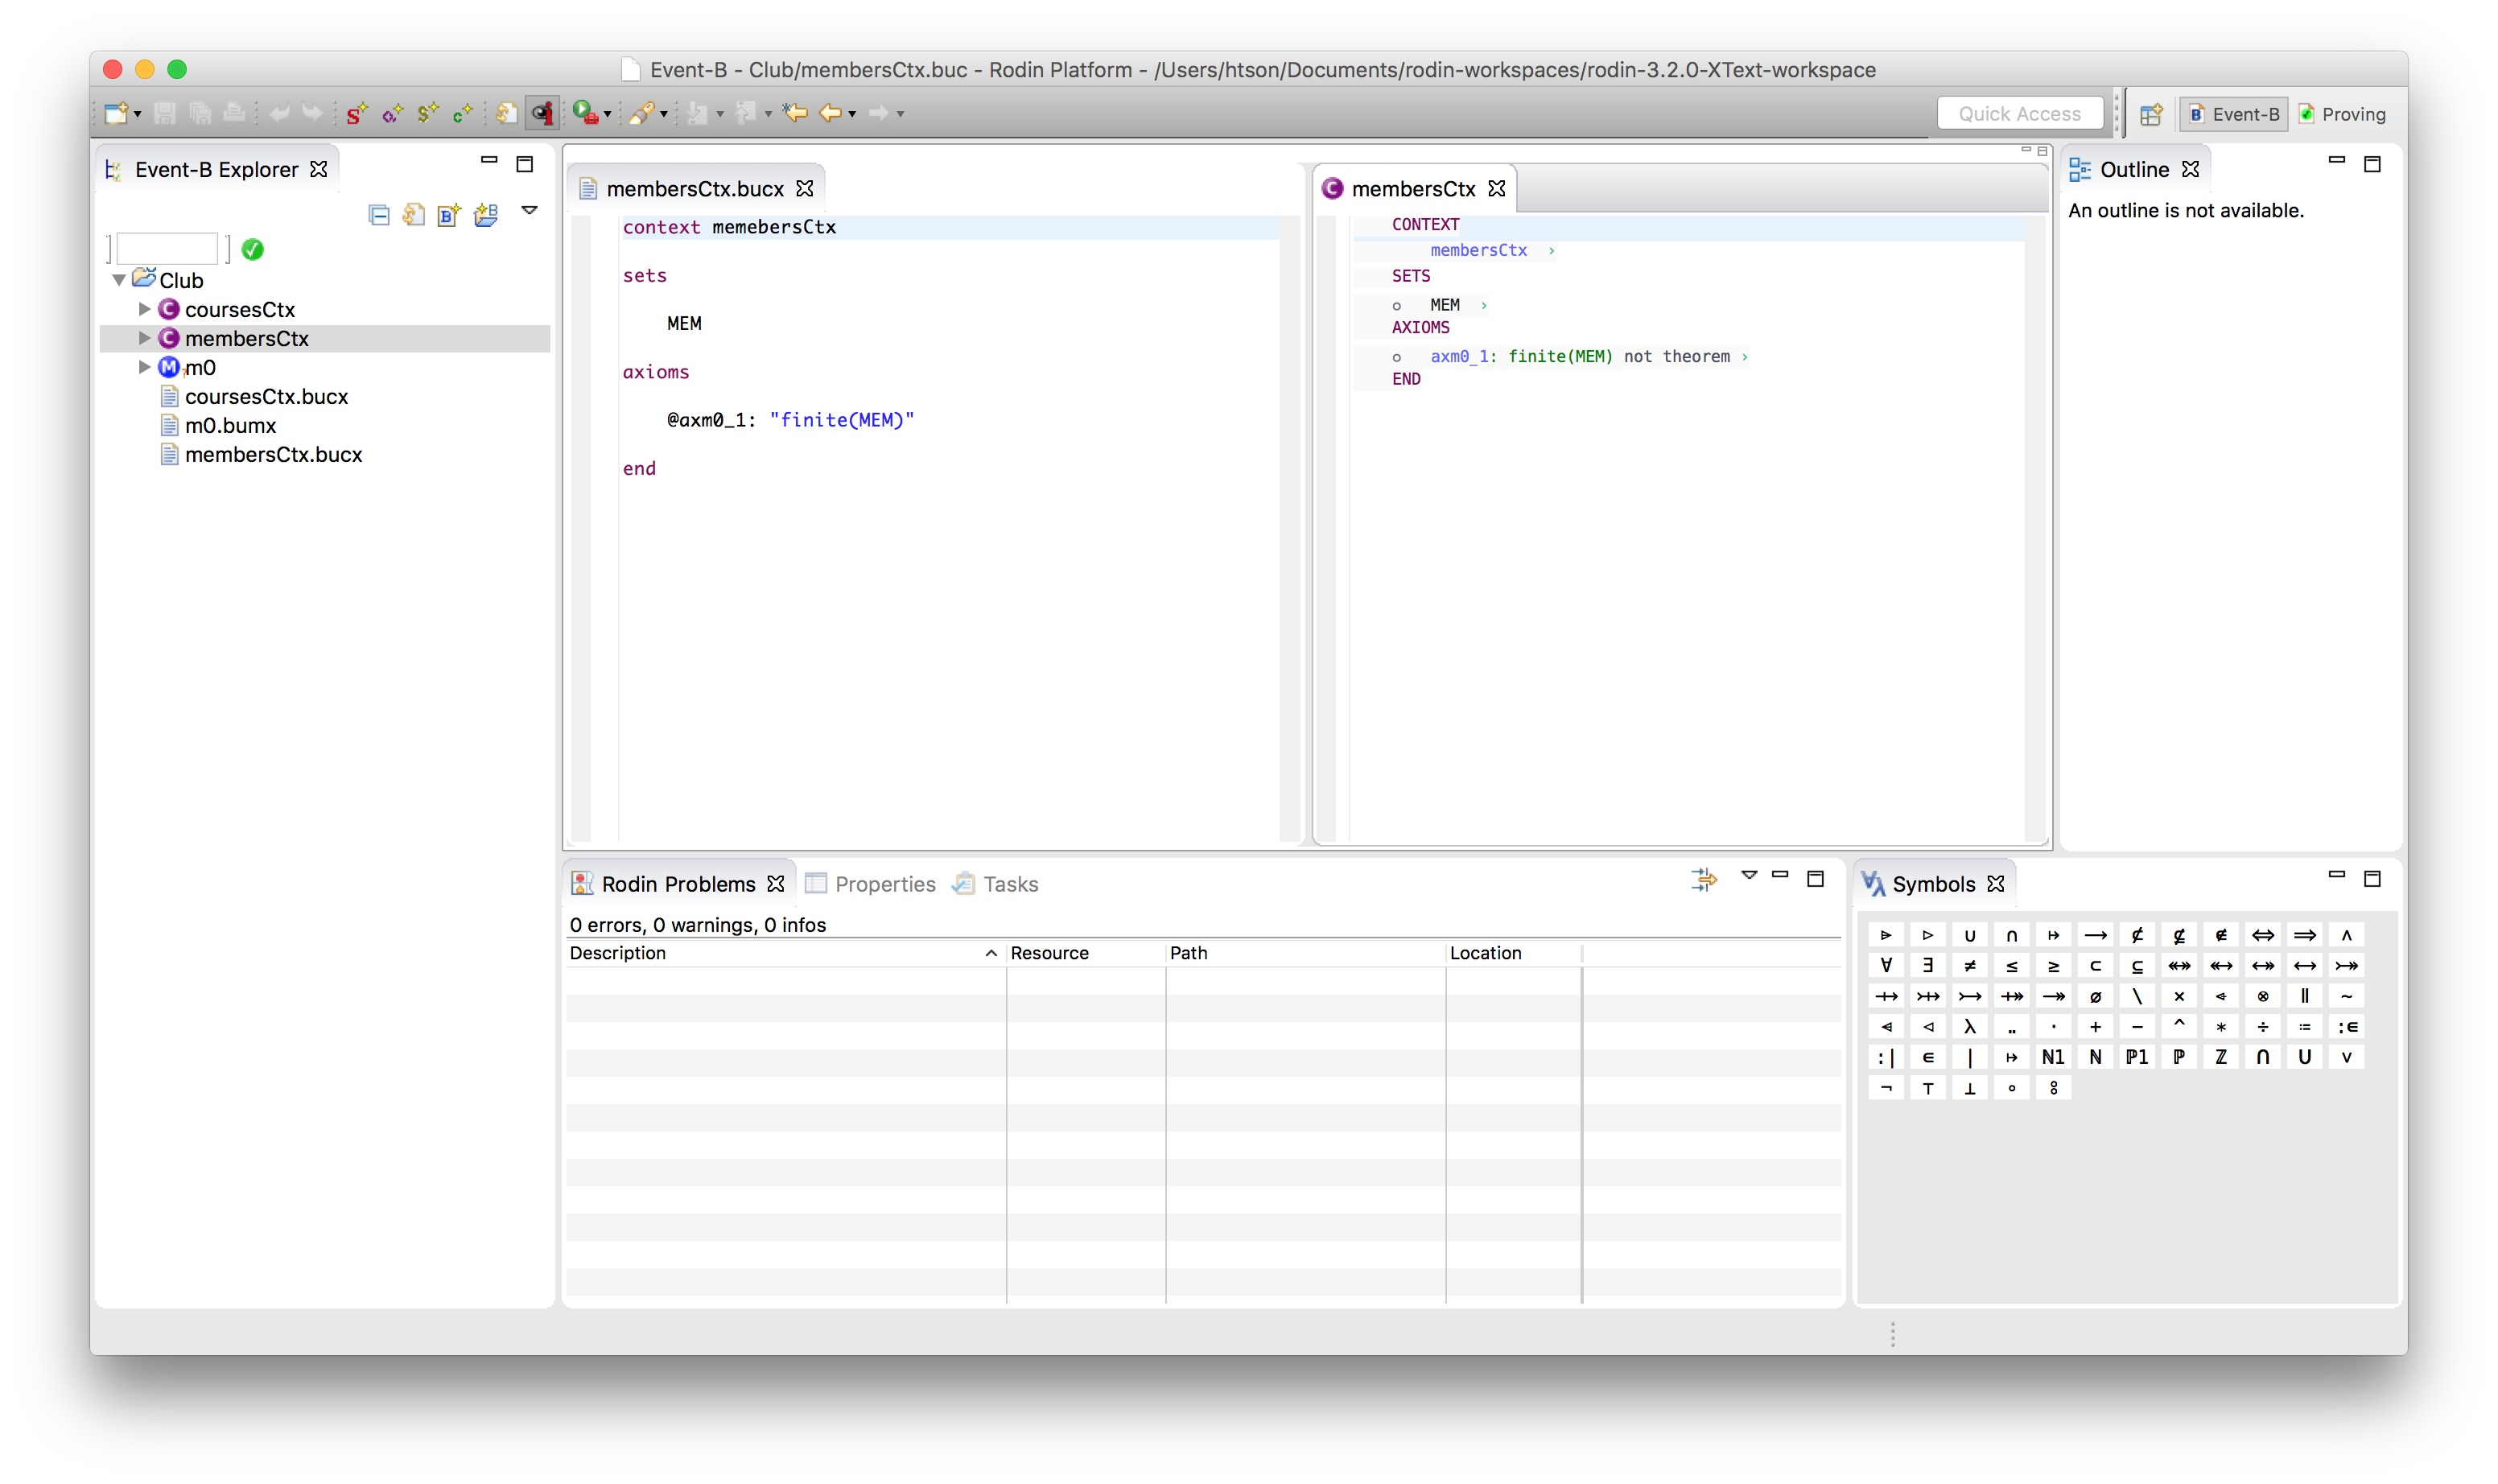
\includegraphics[width=512]{figures/MembersCtx}
    \else
    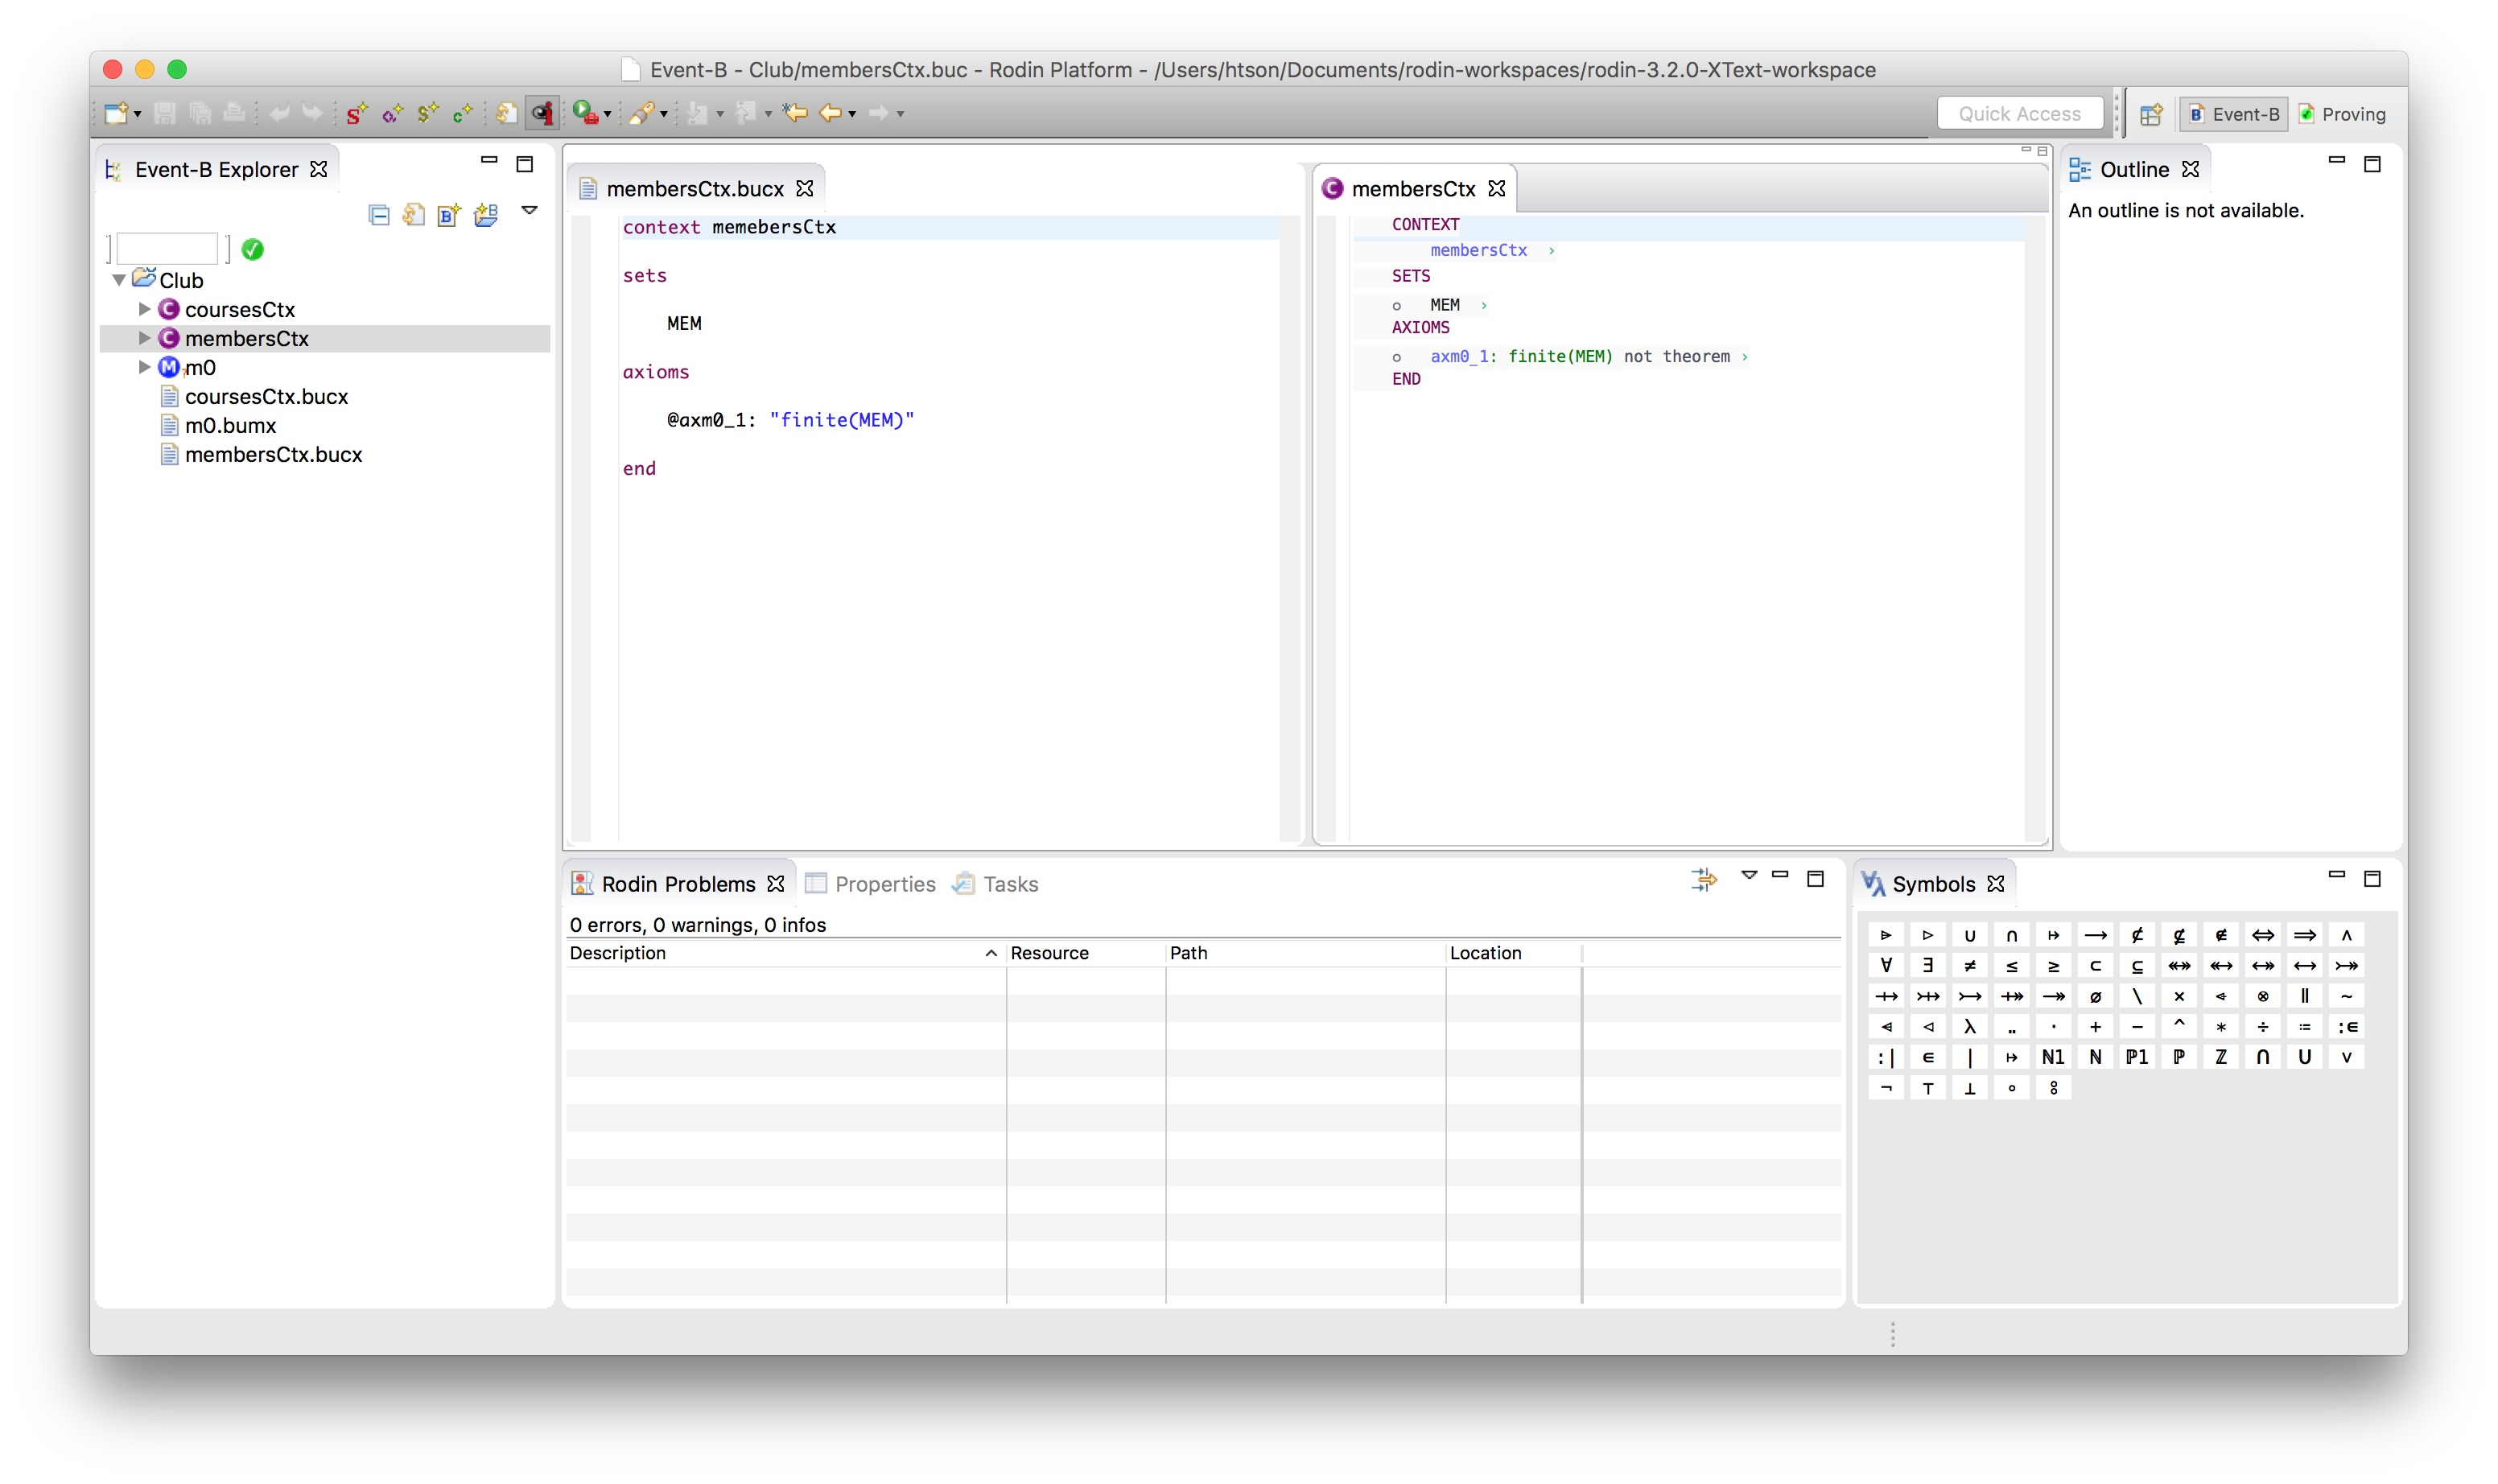
\includegraphics[width=0.9\textwidth]{figures/MembersCtx}
    \endif
    \caption{XContext membersCtx.bucx}
    \label{fig:membersCtx}
  \end{figure}

\paragraph{Task 5.2. Create an extended XContext participantsCtx.bucx}
\textbf{Introduction} The purpose of this sub-task is to create an extended XContext ``participantsCtx.bucx'' within the ``Club'' project.

\begin{description}
\item[Step 1. Create a new XContext participantsCtx.bucx] \textbf{Create a new XContext} named ``participantsCtx.bucx'' using the \emph{New File wizard} (see Figure~\ref{fig:CreateParticipantsCtx}.
  \begin{figure}[!htbp]
    \centering
    \ifdef{PLASTEX}
    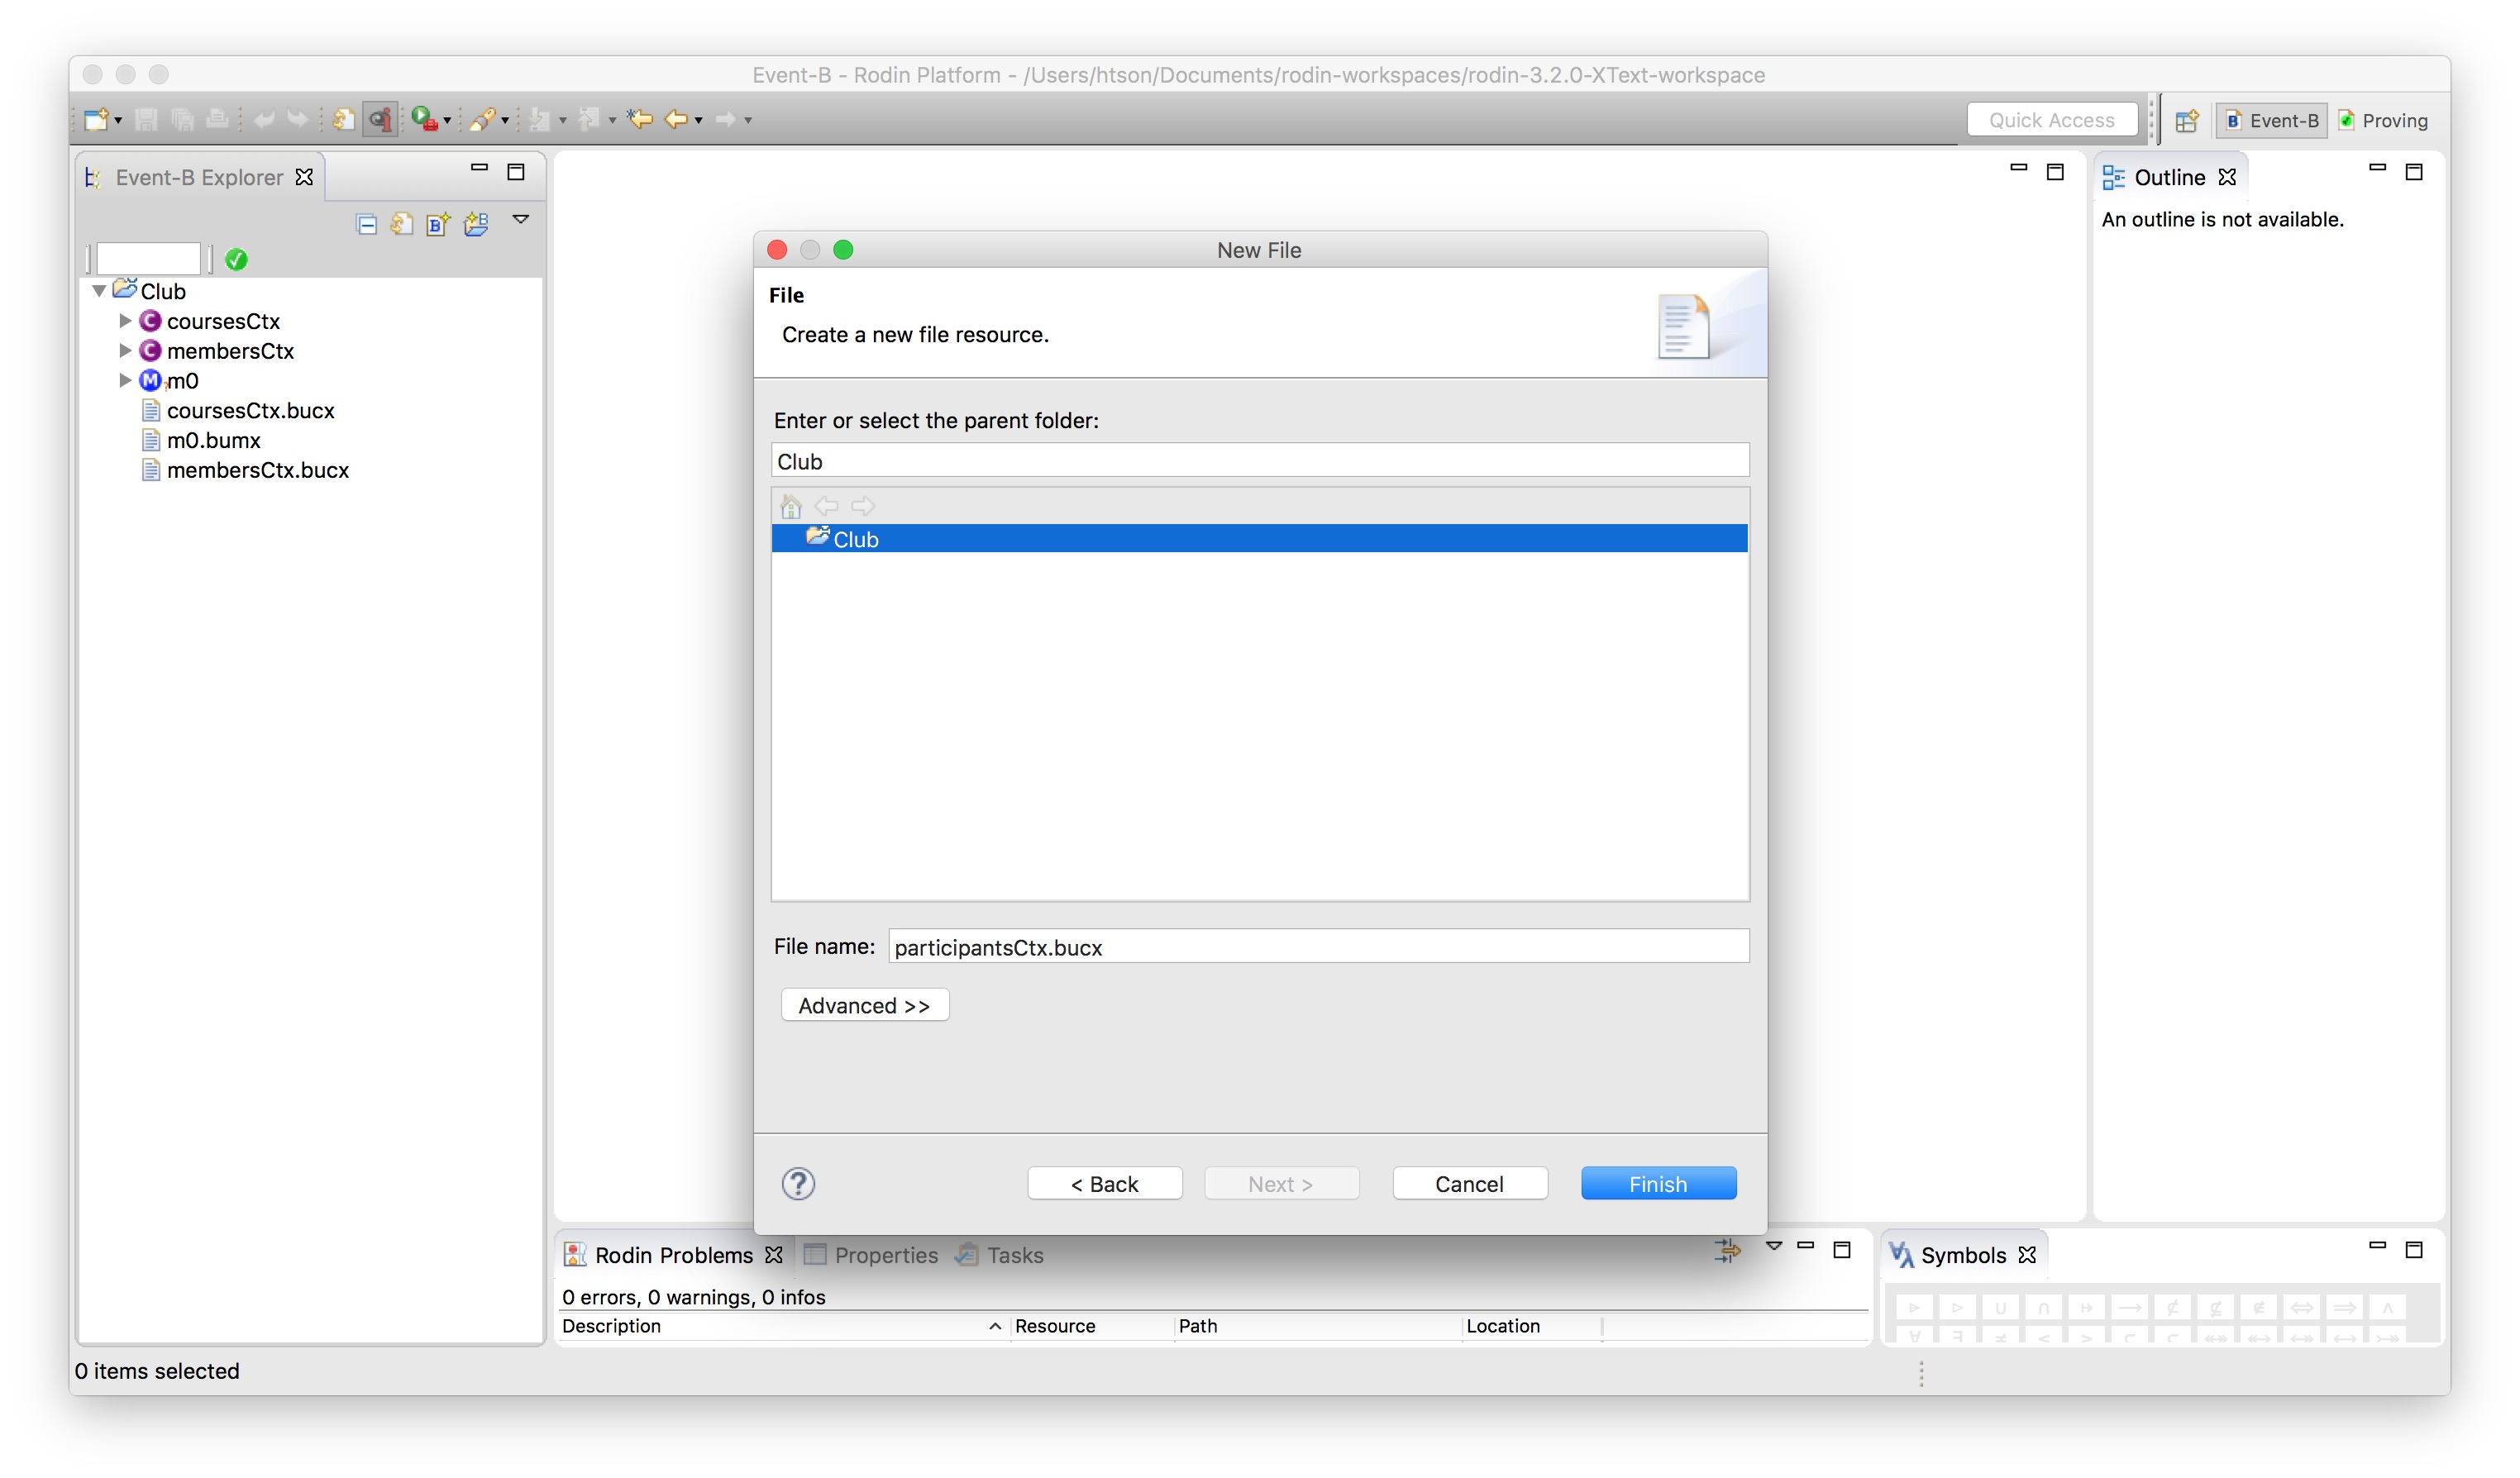
\includegraphics[width=512]{figures/CreateParticipantsCtx}
    \else
    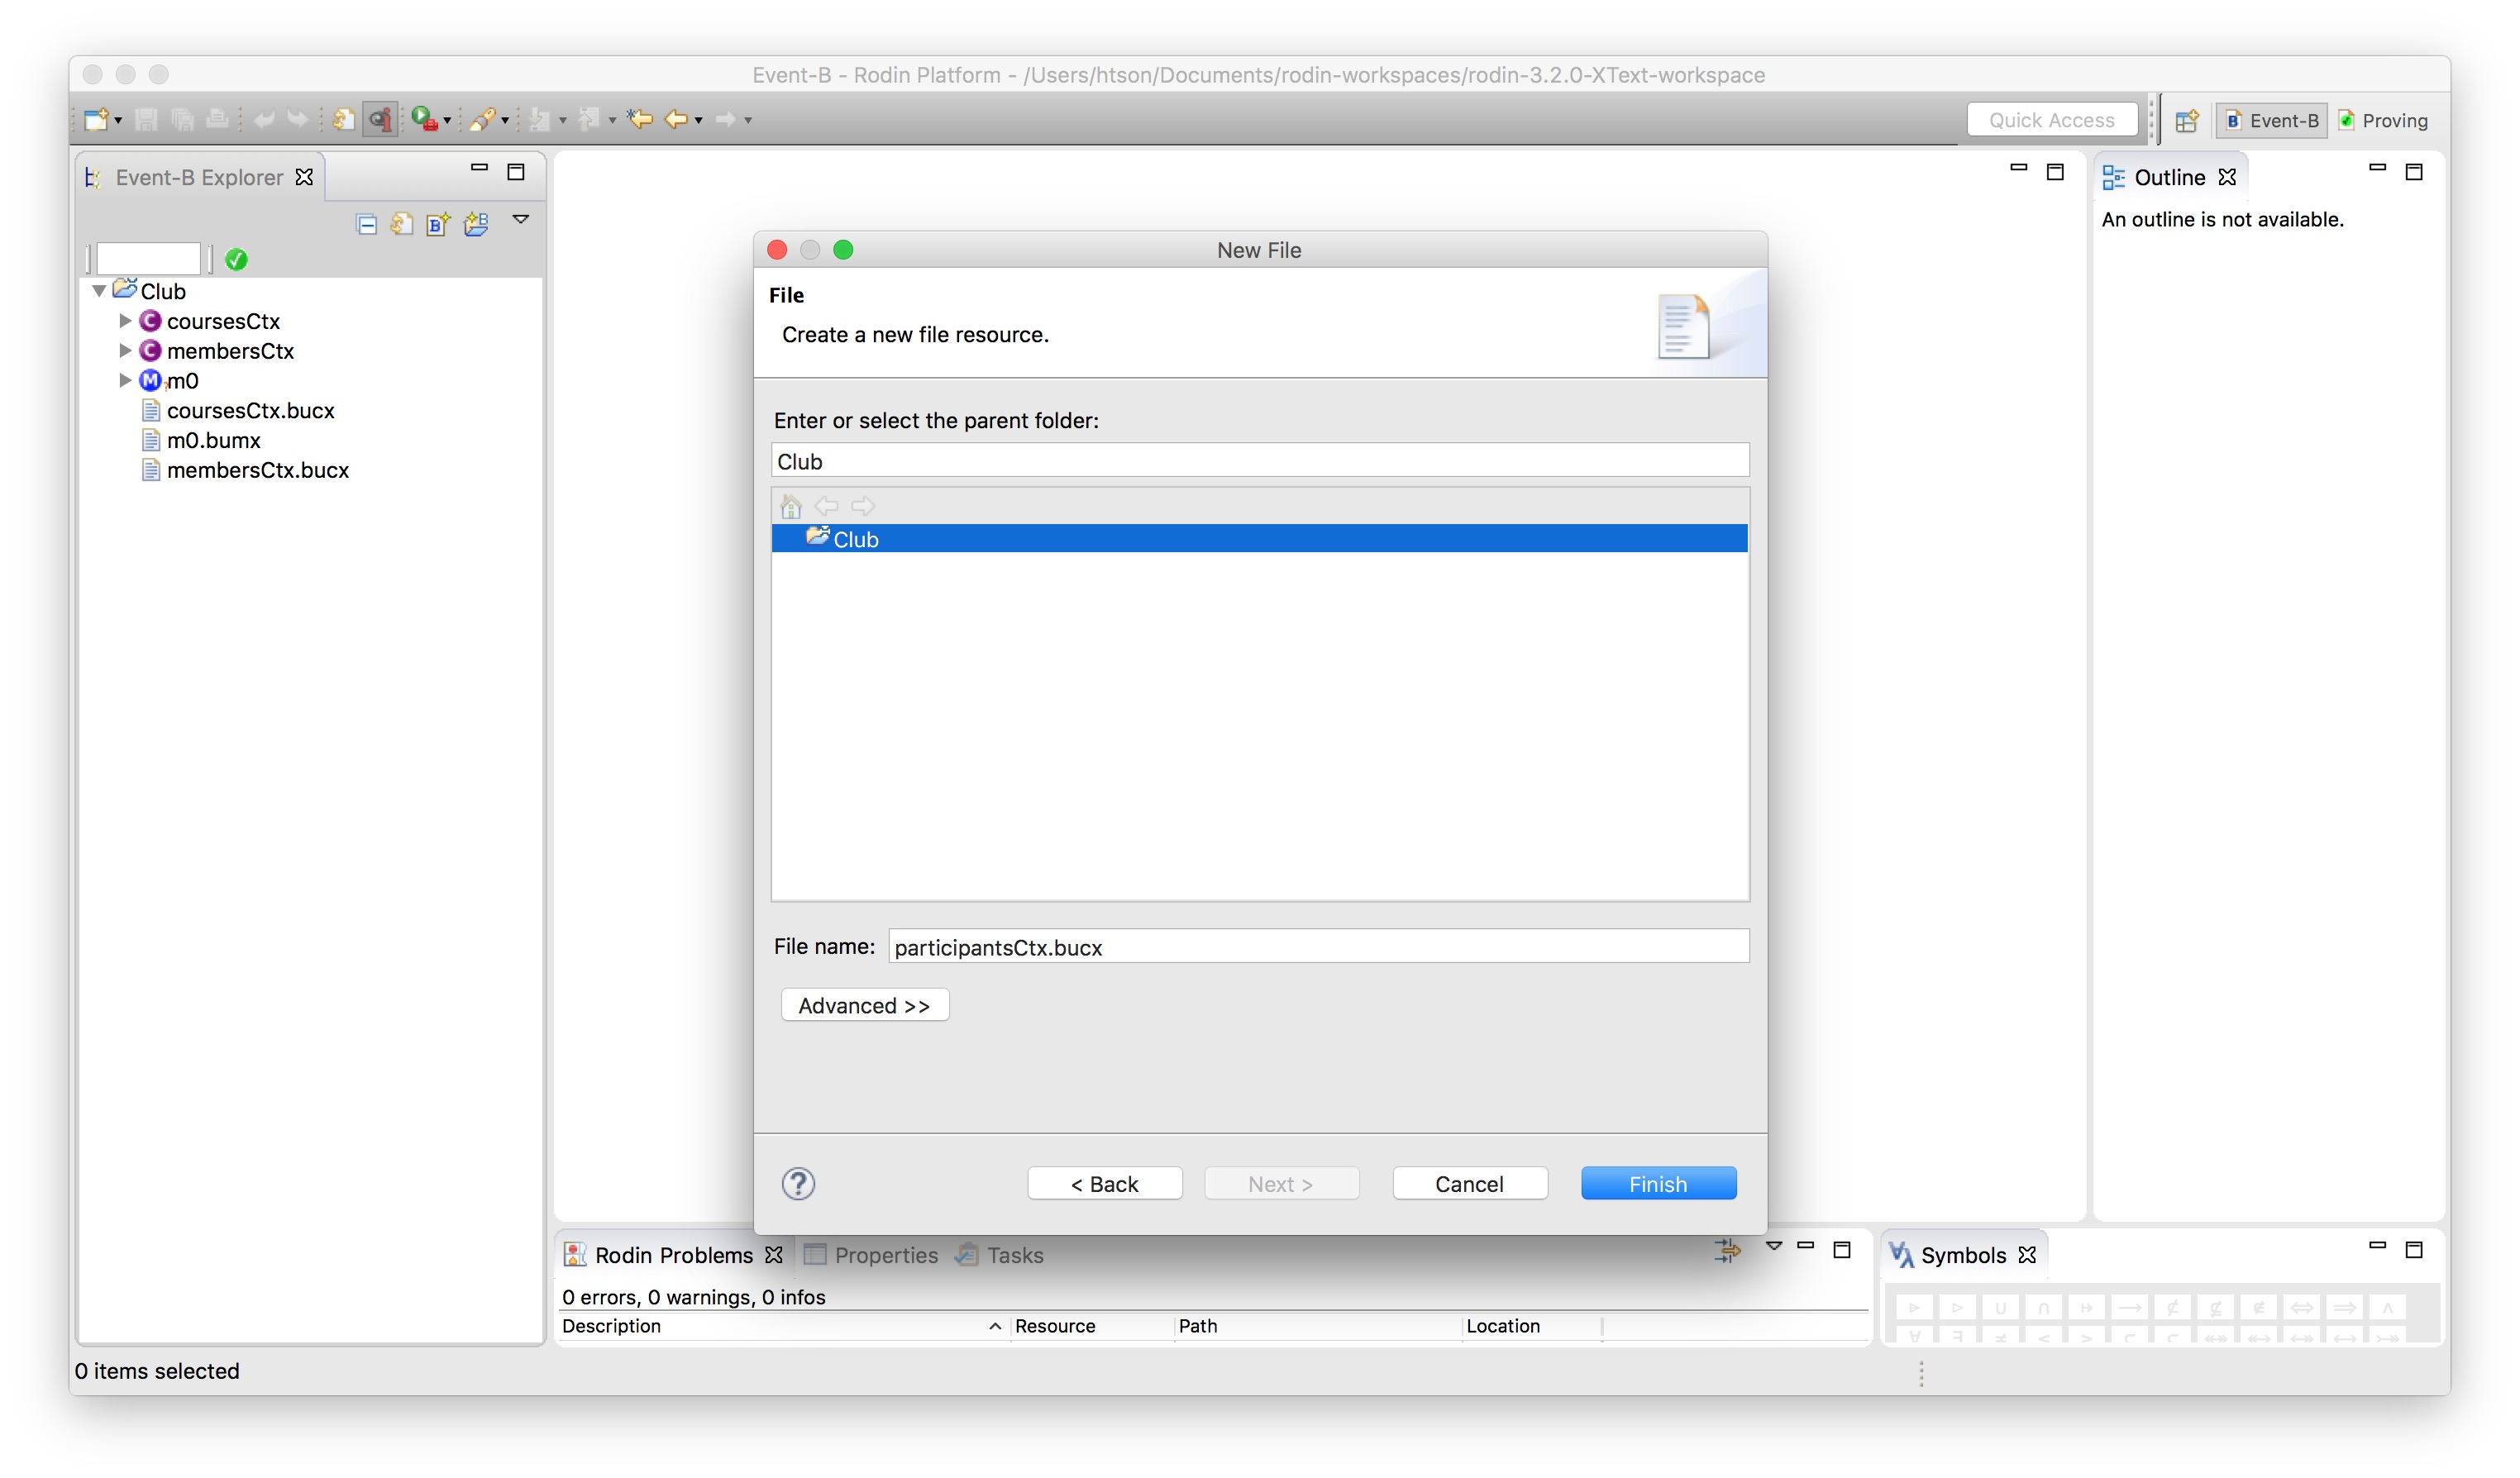
\includegraphics[width=0.9\textwidth]{figures/CreateParticipantsCtx}
    \endif
    \caption{Create participantsCtx.bucx}
    \label{fig:CreateParticipantsCtx}
  \end{figure}

\item[Step 2. Set the content of participantsCtx.bucx] \textbf{Set the content of ``participantsCtx.bucx'' as follows}.
  \begin{center}
    \begin{Bcode}
      \ifdef{PLASTEX}
      \Bcontext{} participantsCtx\\
      \Bextends{} membersCtx\\
      \Bconstants{} PRTCPT\\
      \Baxioms\\
      @axm1_2: PRTCPT ∈ ℙ(MEM)\\
      \Btheorem{} @thm1_1: finite(PRTCPT)\\
      \Bend
      \else
      \Bcontext{} participantsCtx\\
      \Bextends{} membersCtx\\
      \Bconstants{} PRTCPT\\
      \Baxioms\\
      \Btab @axm1_2: \(PRTCPT \in \pow(MEM)\)\\
      \Btab \Btheorem{} @thm1_1: \(\finite(PRTCPT)\)\\
      \Bend
      \endif
    \end{Bcode}
  \end{center}

\item[Step 3. Auto-format the code] \textbf{Automatically format the content of ``participantsCtx.bucx''} by using short-cut (e.g., on Mac OS: Cmd+Shift+F).

\item[Step 4. Save the file] \textbf{Save the file ``participantsCtx.bucx''}.
\end{description}

\textbf{Conclusion} By now, the XContext ``participantsCtx.bucx'' and the corresponding Rodin Context ``participantsCtx'' should be visible in the Event-B Explorer (see Figure~\ref{fig:ParticipantsCtx}).
  \begin{figure}[!htbp]
    \centering
    \ifdef{PLASTEX}
    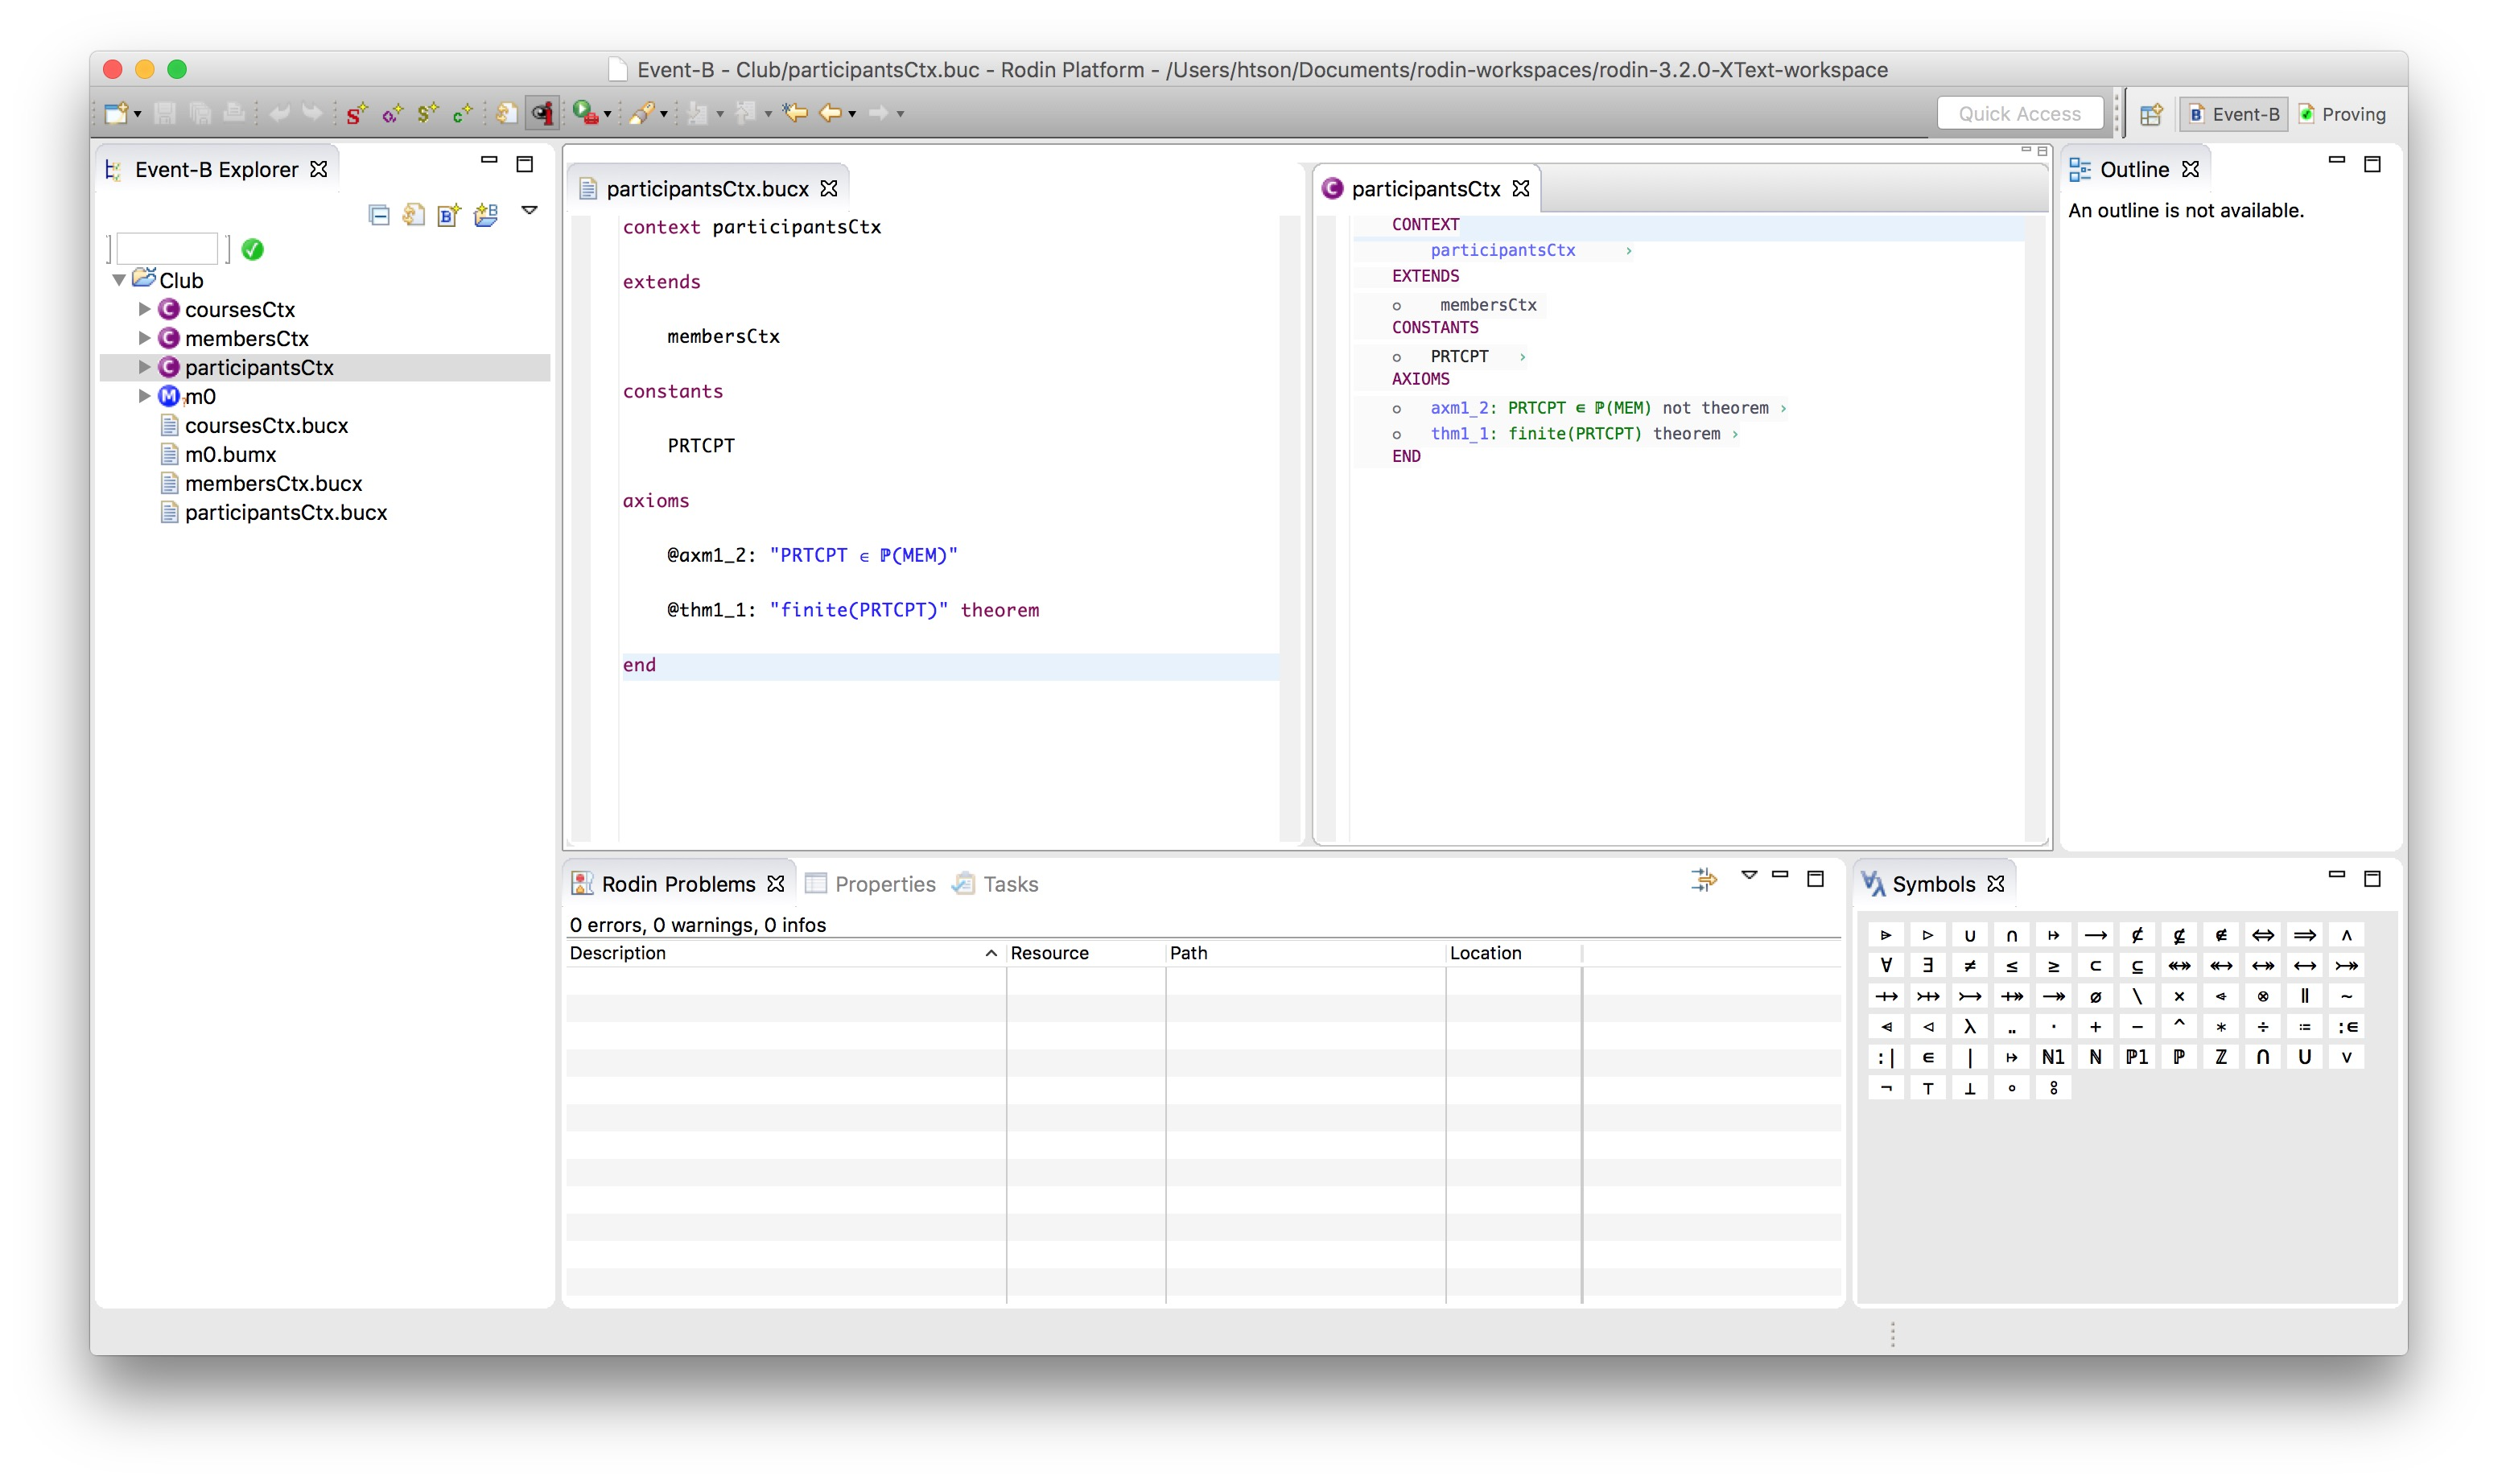
\includegraphics[width=512]{figures/ParticipantsCtx}
    \else
    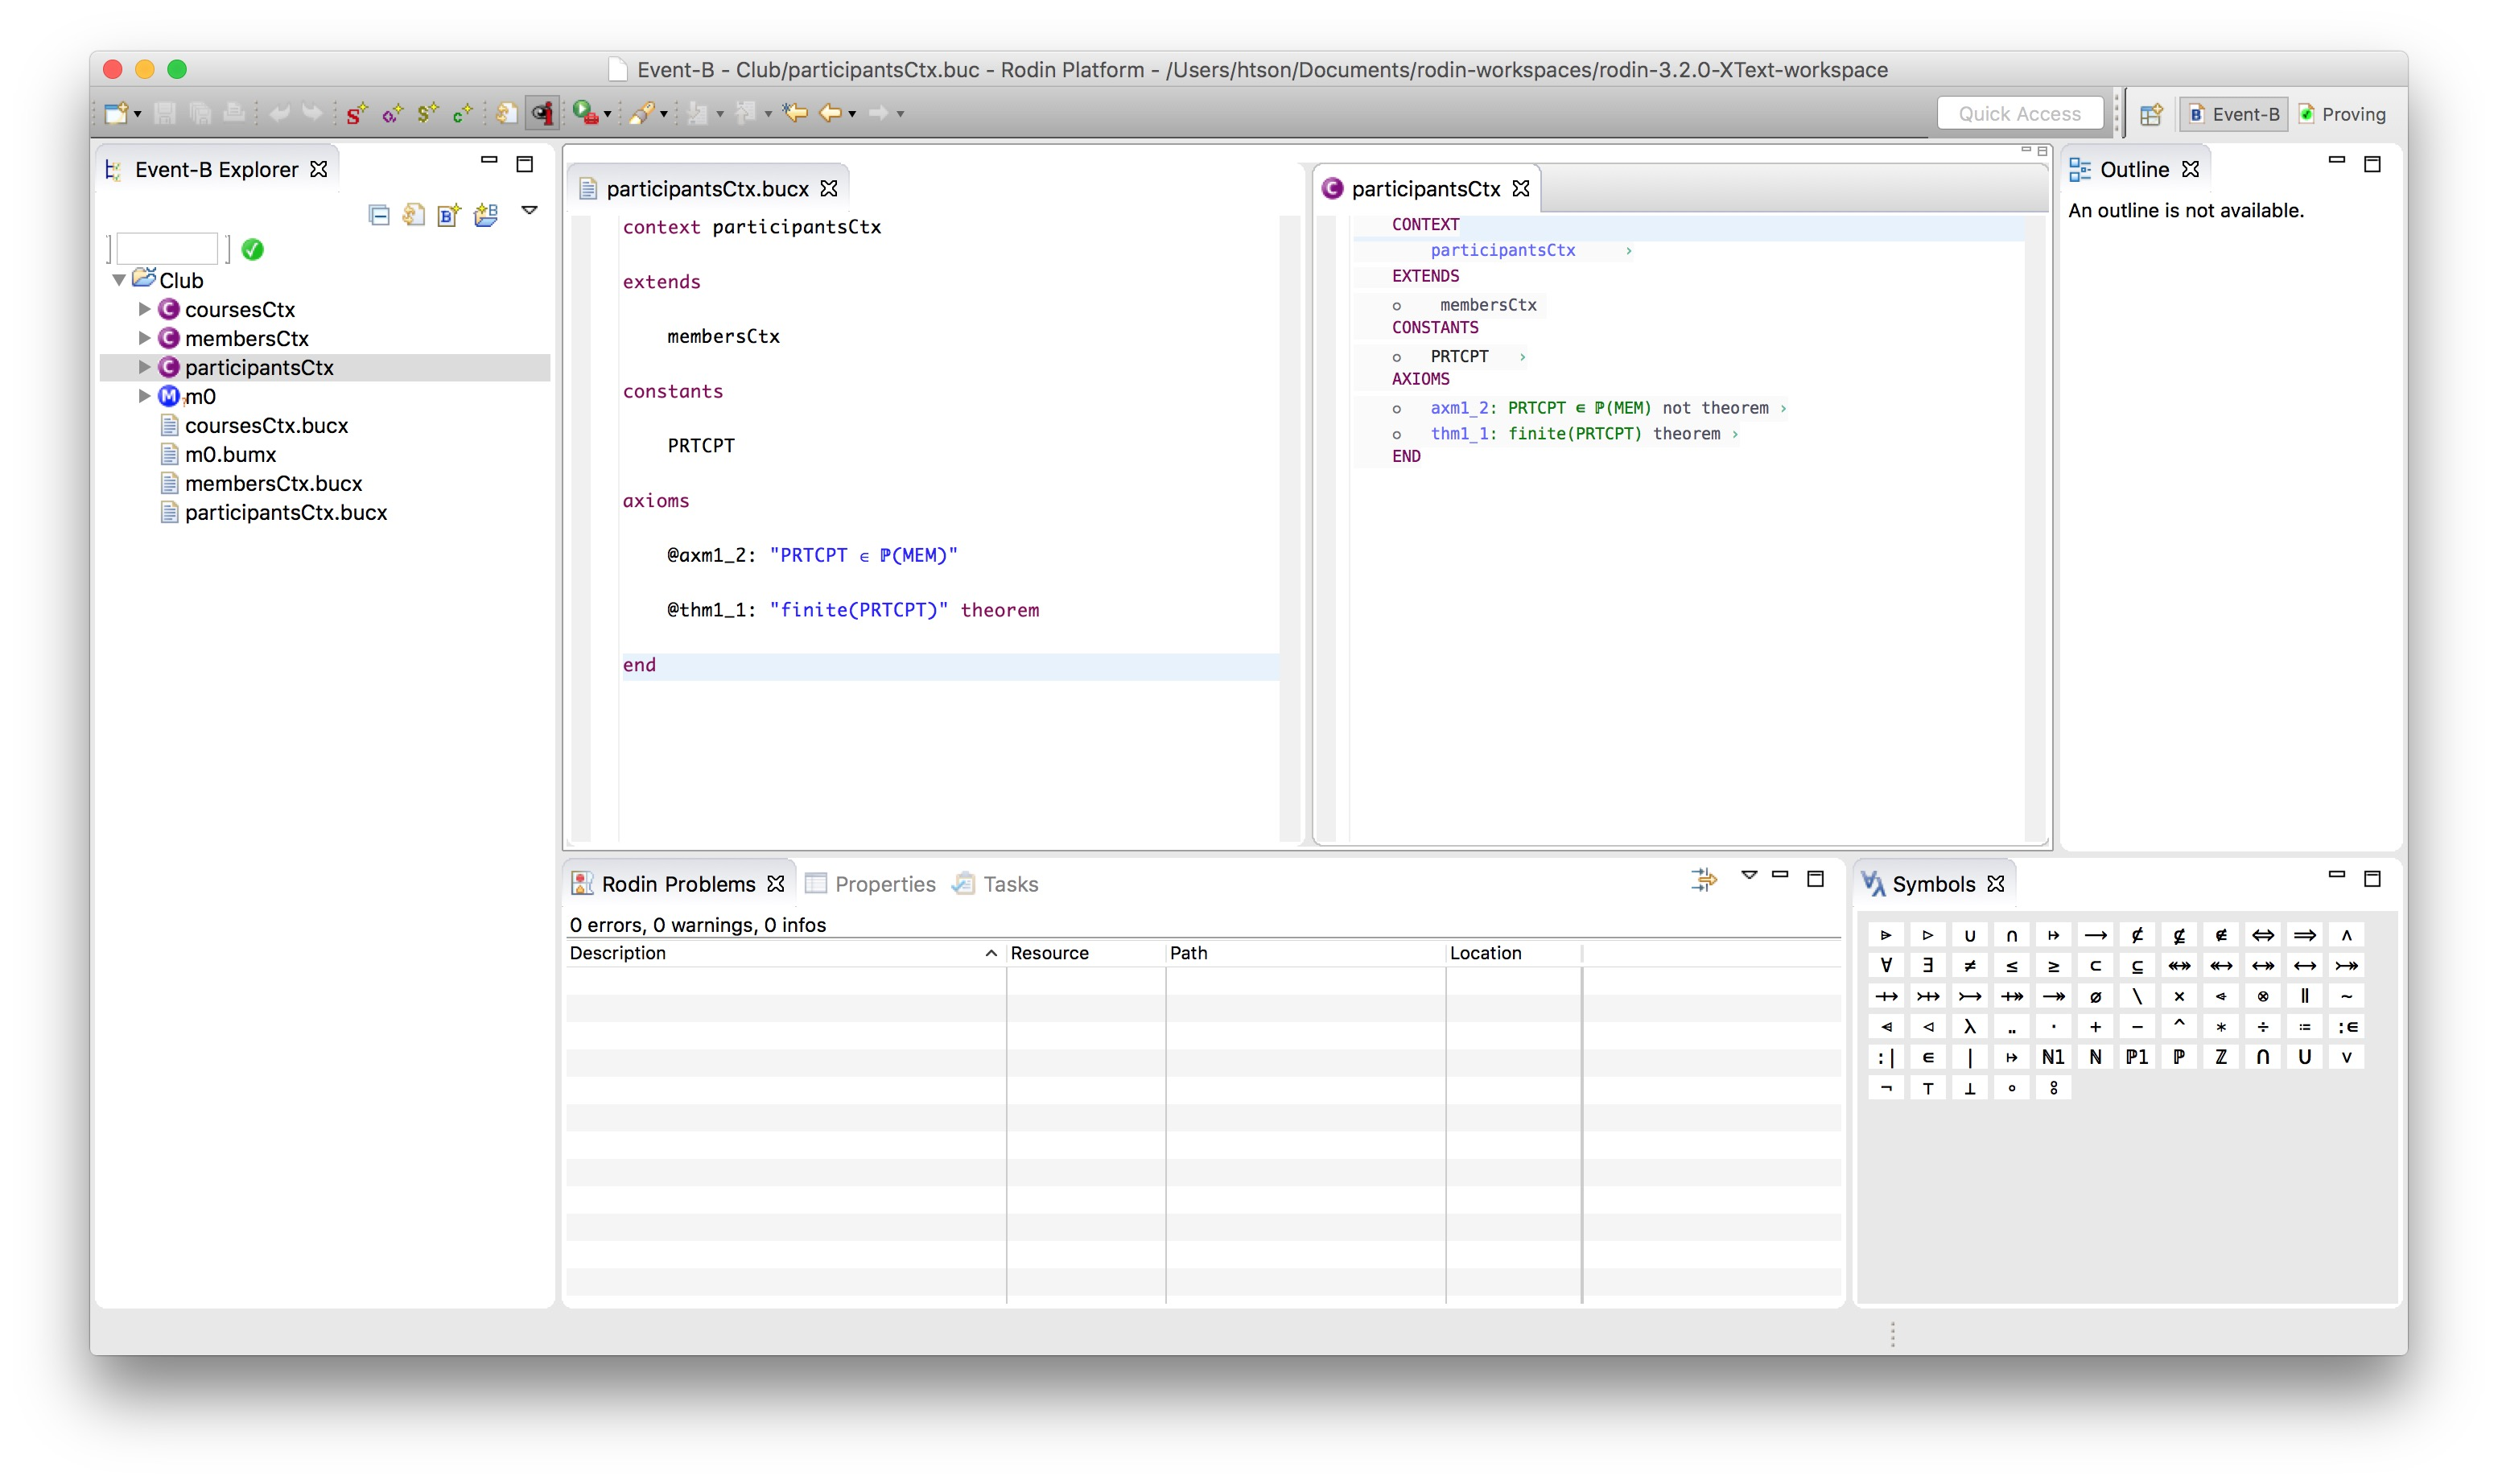
\includegraphics[width=0.9\textwidth]{figures/ParticipantsCtx}
    \endif
    \caption{XContext participantsCtx.bucx}
    \label{fig:ParticipantsCtx}
  \end{figure}

\paragraph{Task 5.3. Create an extended XContext instructorsCtx.bucx}
\textbf{Introduction} The purpose of this sub-task is to create an extended XContext ``instructorsCtx.bucx'' within the ``Club'' project.
\begin{description}
\item[Step 1. Create a new XContext instructorsCtx.bucx] \textbf{Create a new XContext} named ``instructorsCtx.bucx'' using the \emph{New File wizard} (see Figure~\ref{fig:CreateInstructorsCtx}.
  \begin{figure}[!htbp]
    \centering
    \ifdef{PLASTEX}
    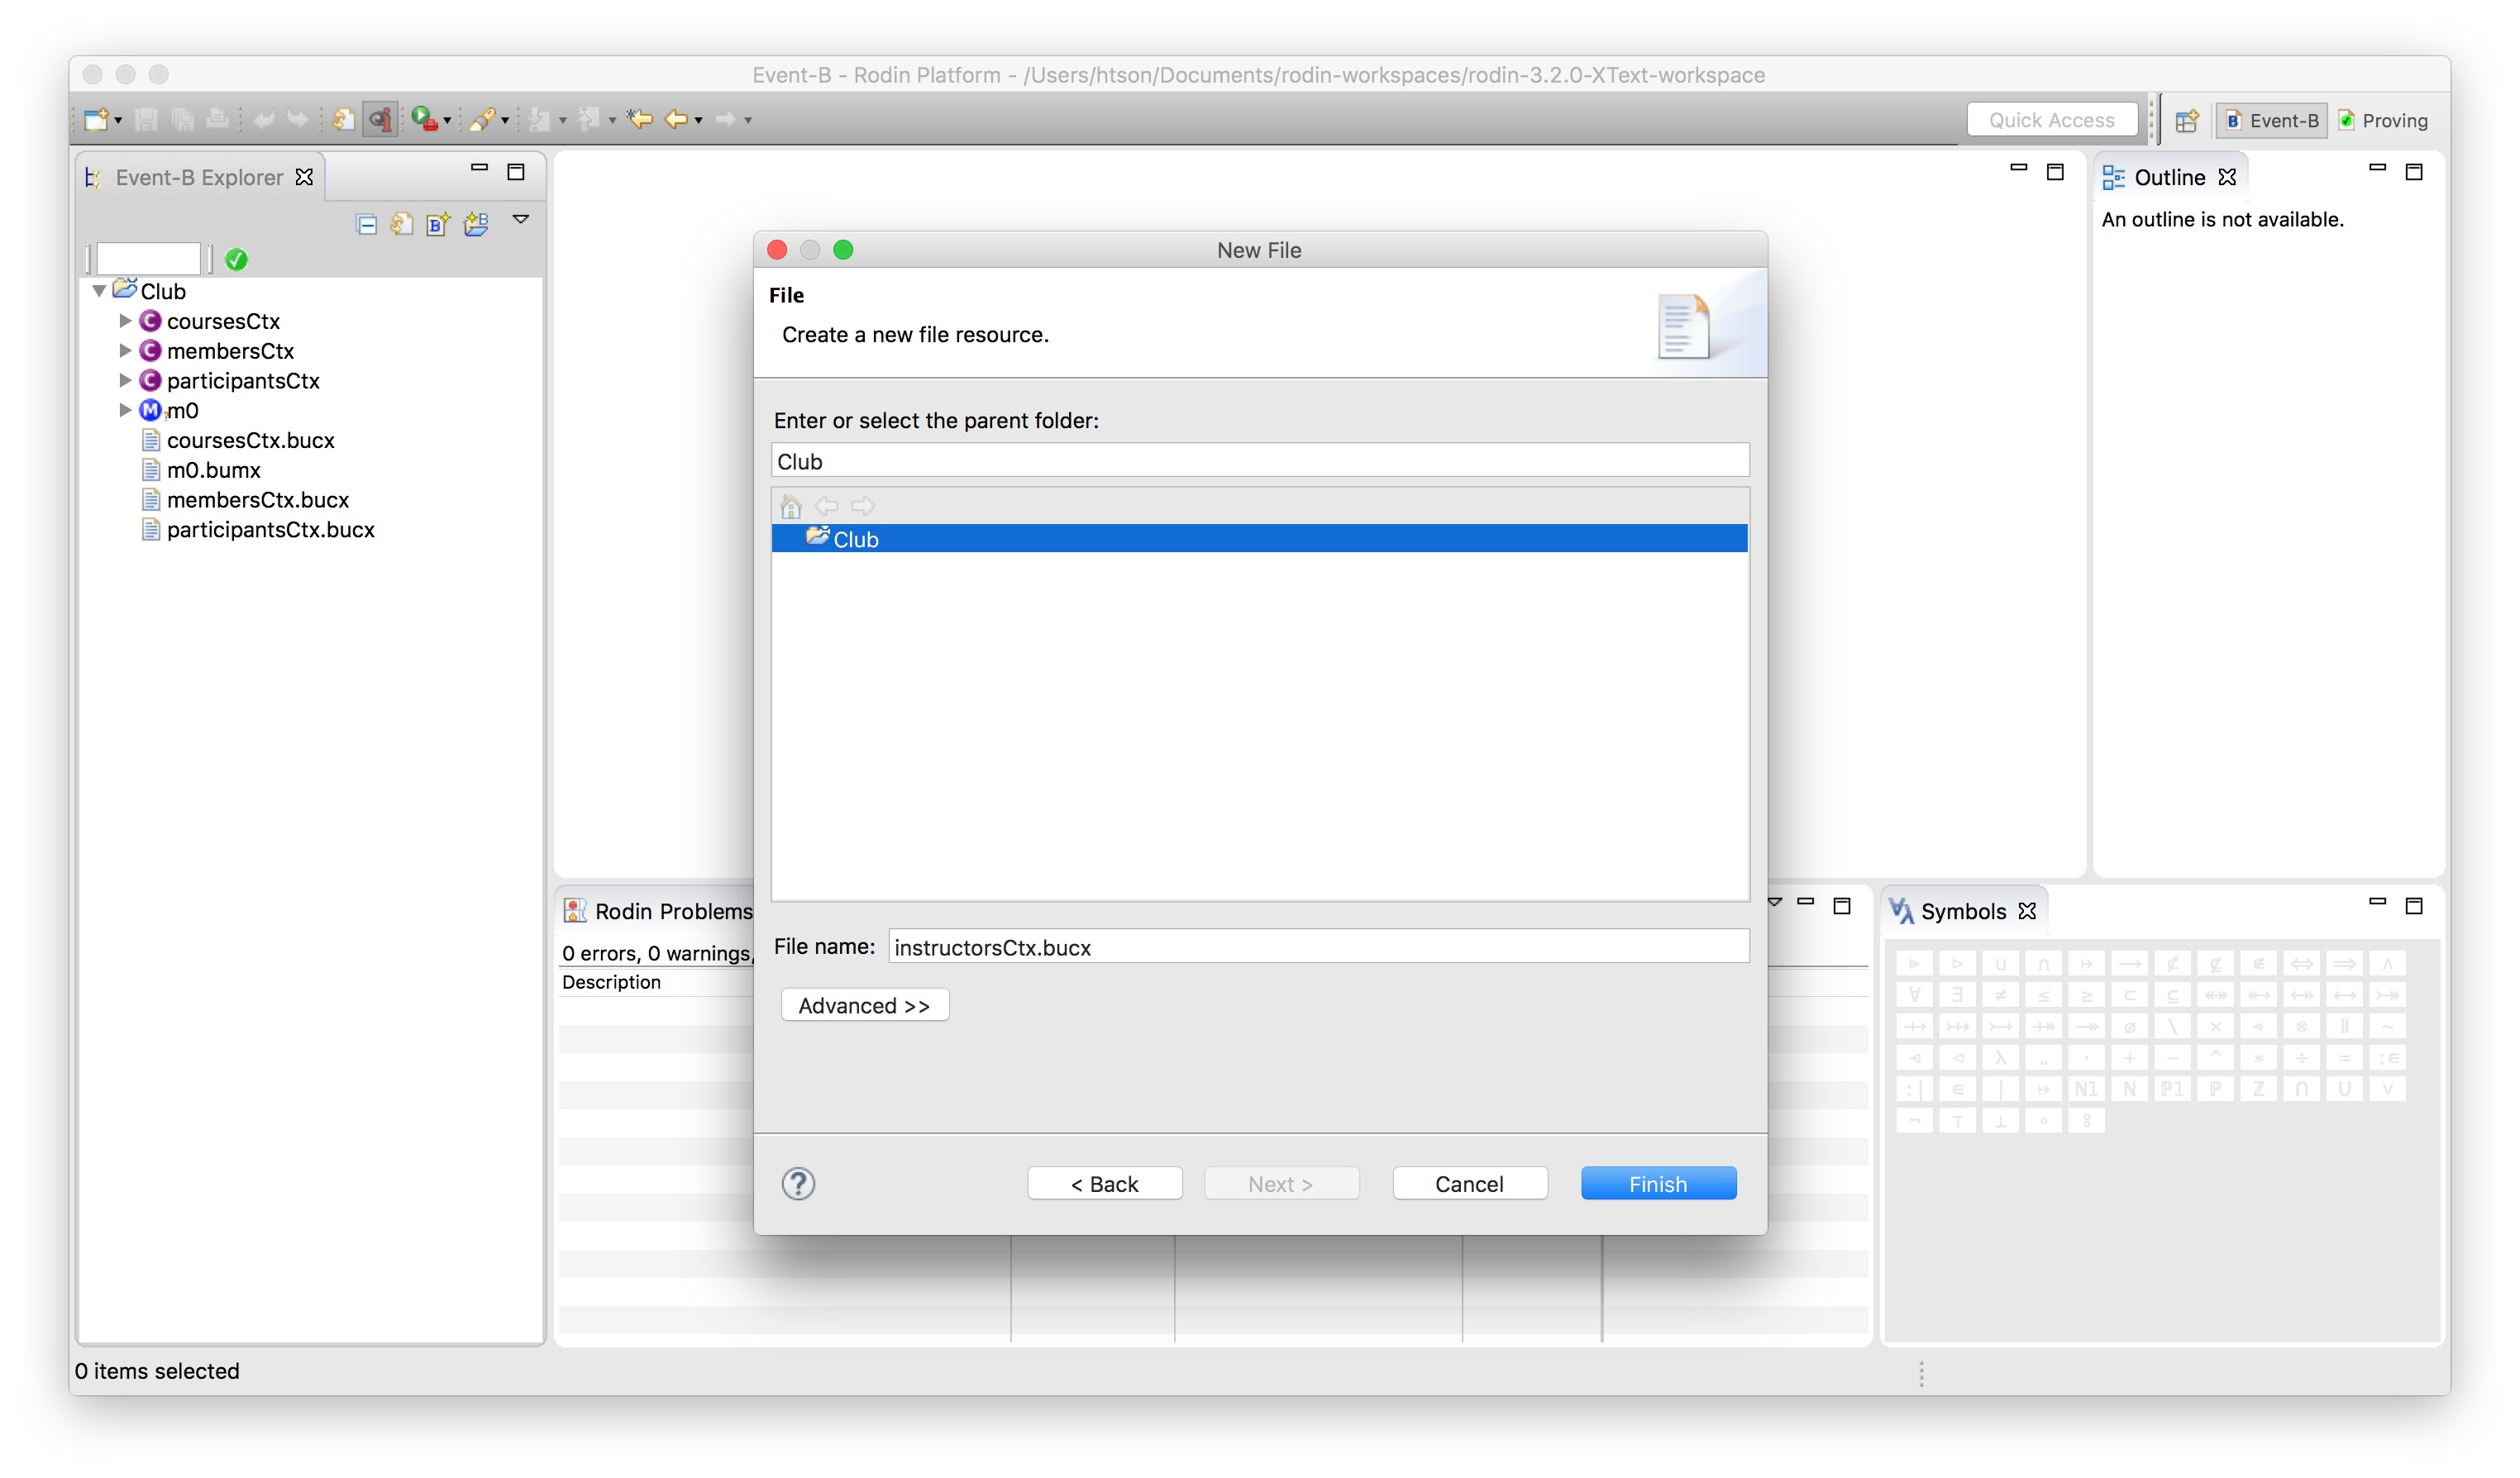
\includegraphics[width=512]{figures/CreateInstructorsCtx}
    \else
    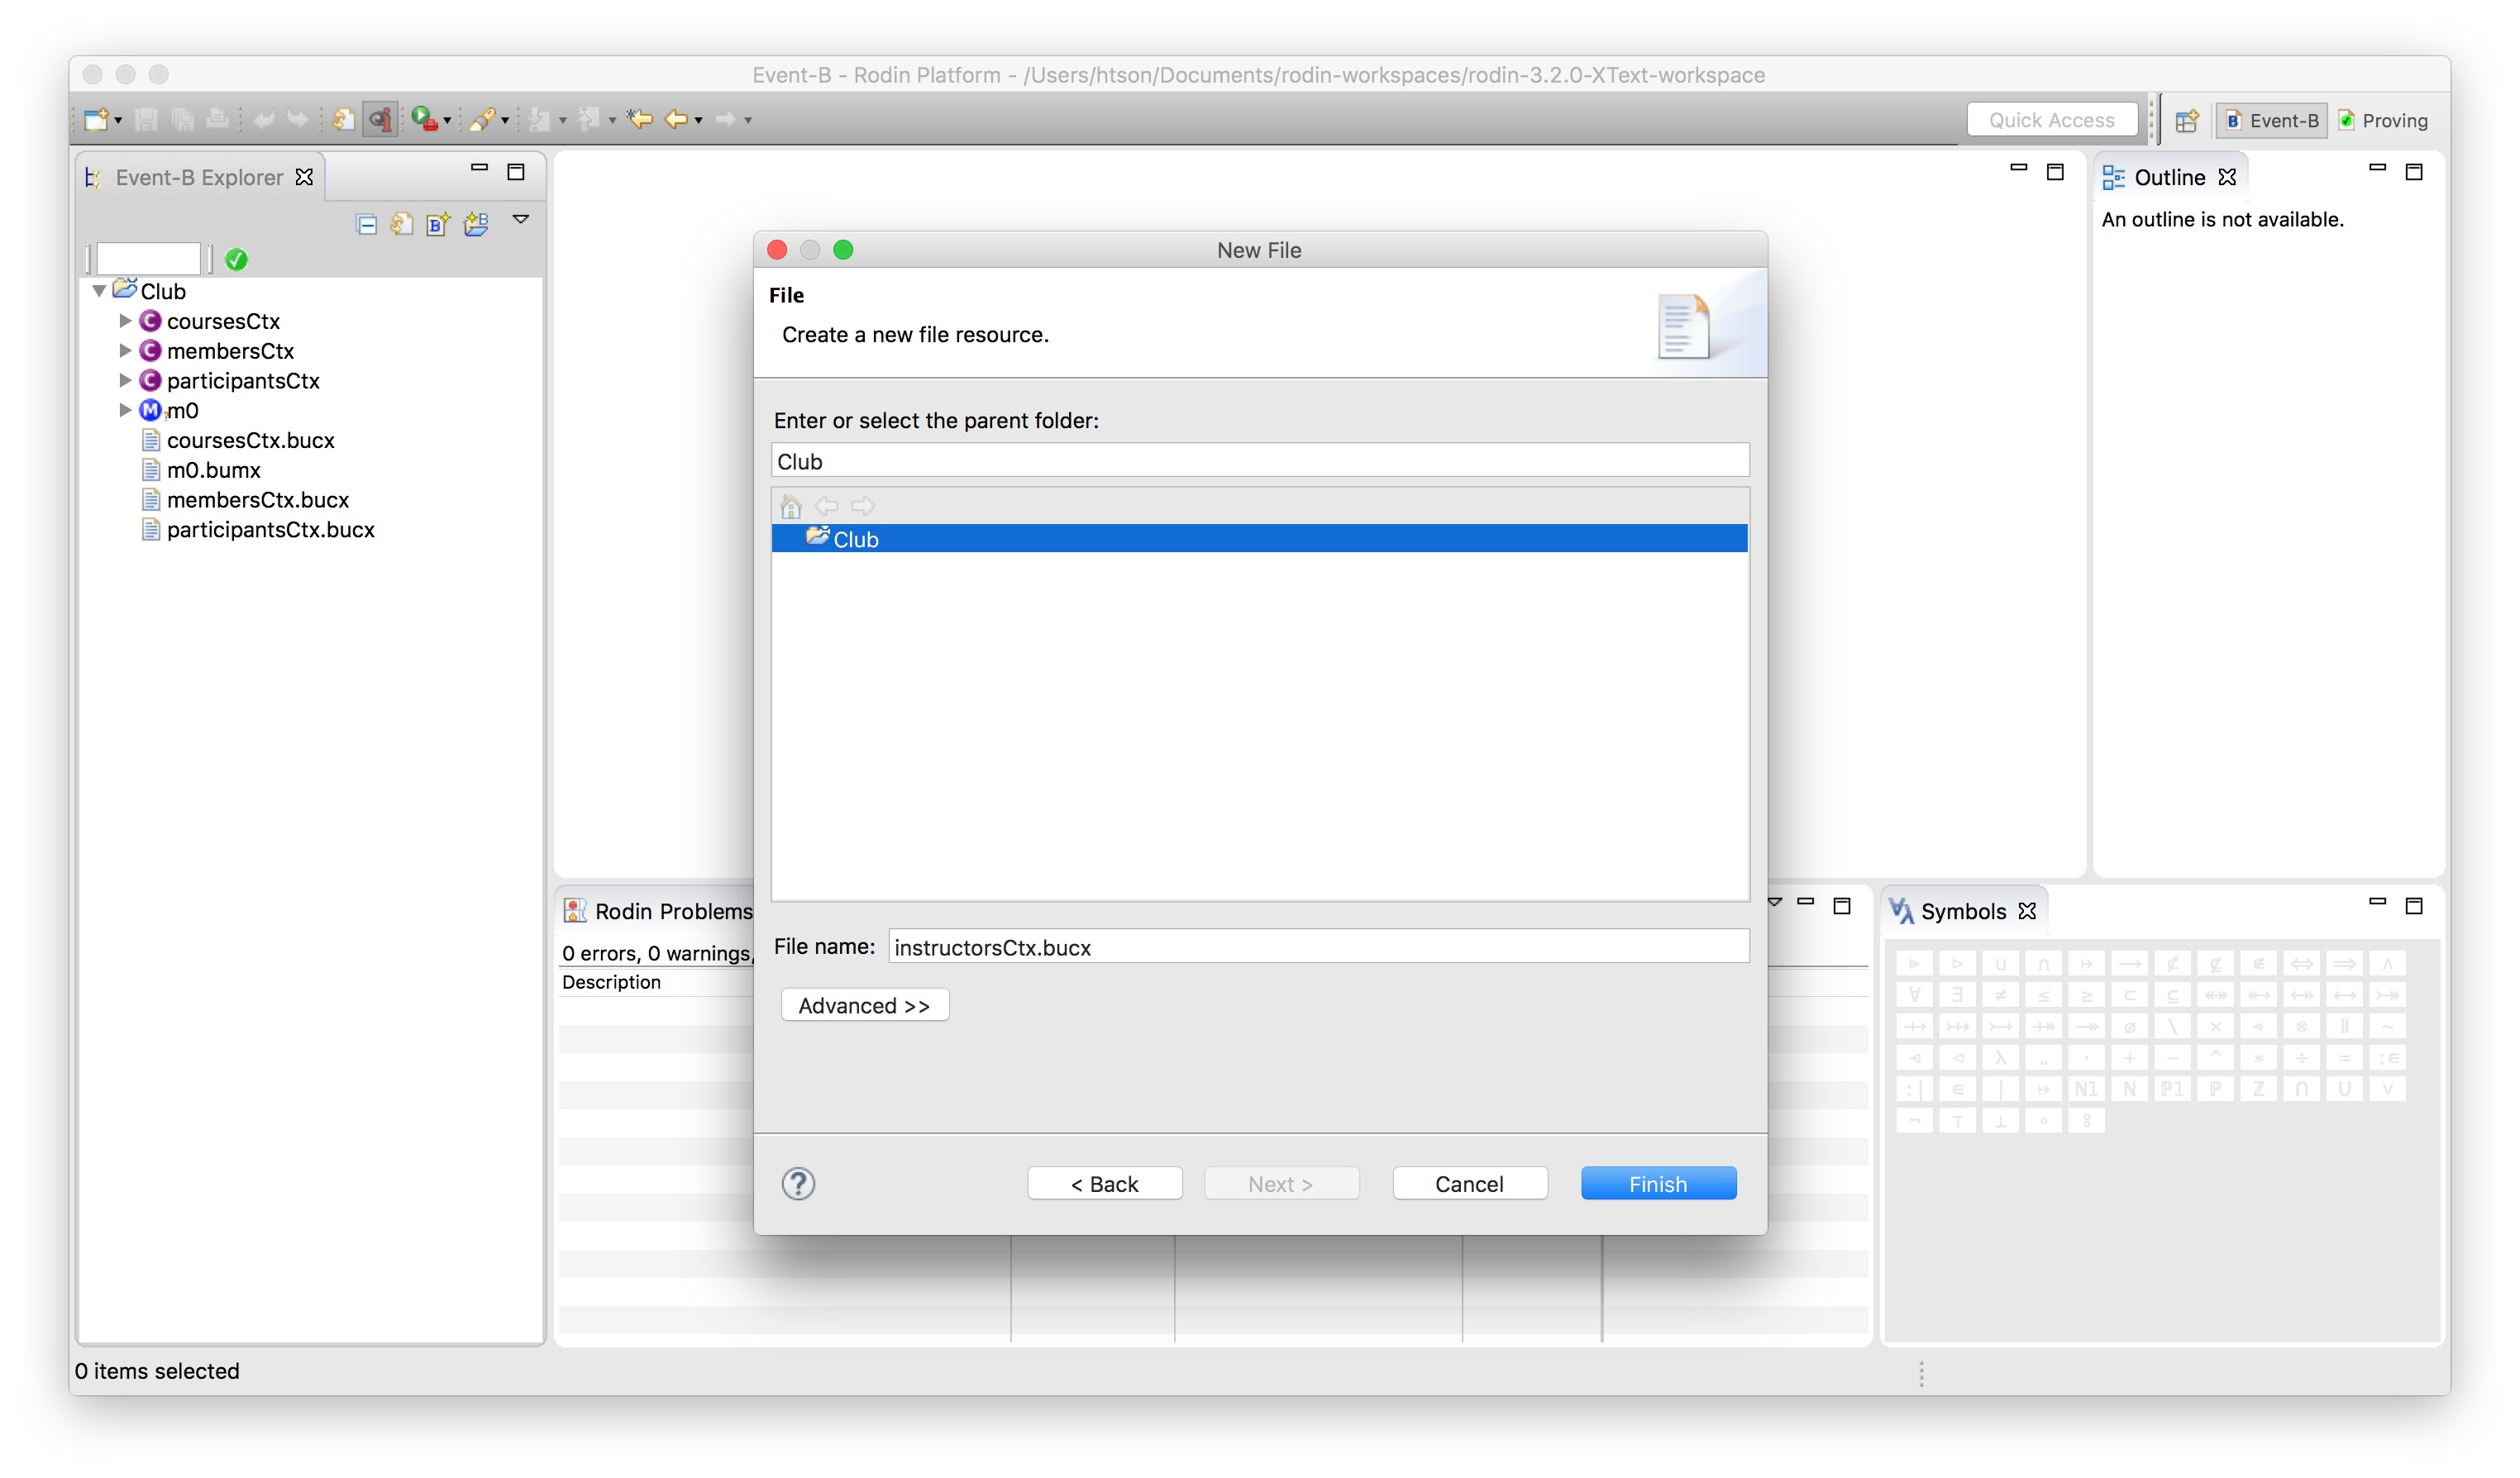
\includegraphics[width=0.9\textwidth]{figures/CreateInstructorsCtx}
    \endif
    \caption{Create instructorsCtx.bucx}
    \label{fig:CreateInstructorsCtx}
  \end{figure}

\item[Step 2. Set the content of instructorsCtx.bucx] \textbf{Set the content of ``instructorsCtx.bucx'' as follows}.
  \begin{center}
    \begin{Bcode}
      \ifdef{PLASTEX}
      \Bcontext{} instructorsCtx\\
      \Bextends{} membersCtx coursesCtx\\
      \Bconstants{} INSTR instrs\\
      \Baxioms\\
      @axm1_3: INSTR ∈ ℙ(MEM)\\
      @axm1_4: instrs ∈ CRS → INSTR\\
      \Bend
      \else
      \Bcontext{} instructorsCtx\\
      \Bextends{} membersCtx coursesCtx\\
      \Bconstants{} INSTR instrs\\
      \Baxioms\\
      \Btab @axm1_3: \(INSTR \in \pow(MEM)\)\\
      \Btab @axm1_4: \(instrs \in CRS \tfun INSTR\)\\
      \Bend
      \endif
    \end{Bcode}
  \end{center}

\item[Step 3. Auto-format the code] \textbf{Automatically format the content of ``intructorsCtx.bucx''} by using short-cut (e.g., on Mac OS: Cmd+Shift+F).

\item[Step 4. Save the file] \textbf{Save the file ``instructorsCtx.bucx''}.
\end{description}

\textbf{Conclusion} By now, the XContext ``instructorsCtx.bucx'' and the corresponding Rodin Context ``instructorsCtx'' should be visible in the Event-B Explorer (see Figure.
  \begin{figure}[!htbp]
    \centering
    \ifdef{PLASTEX}
    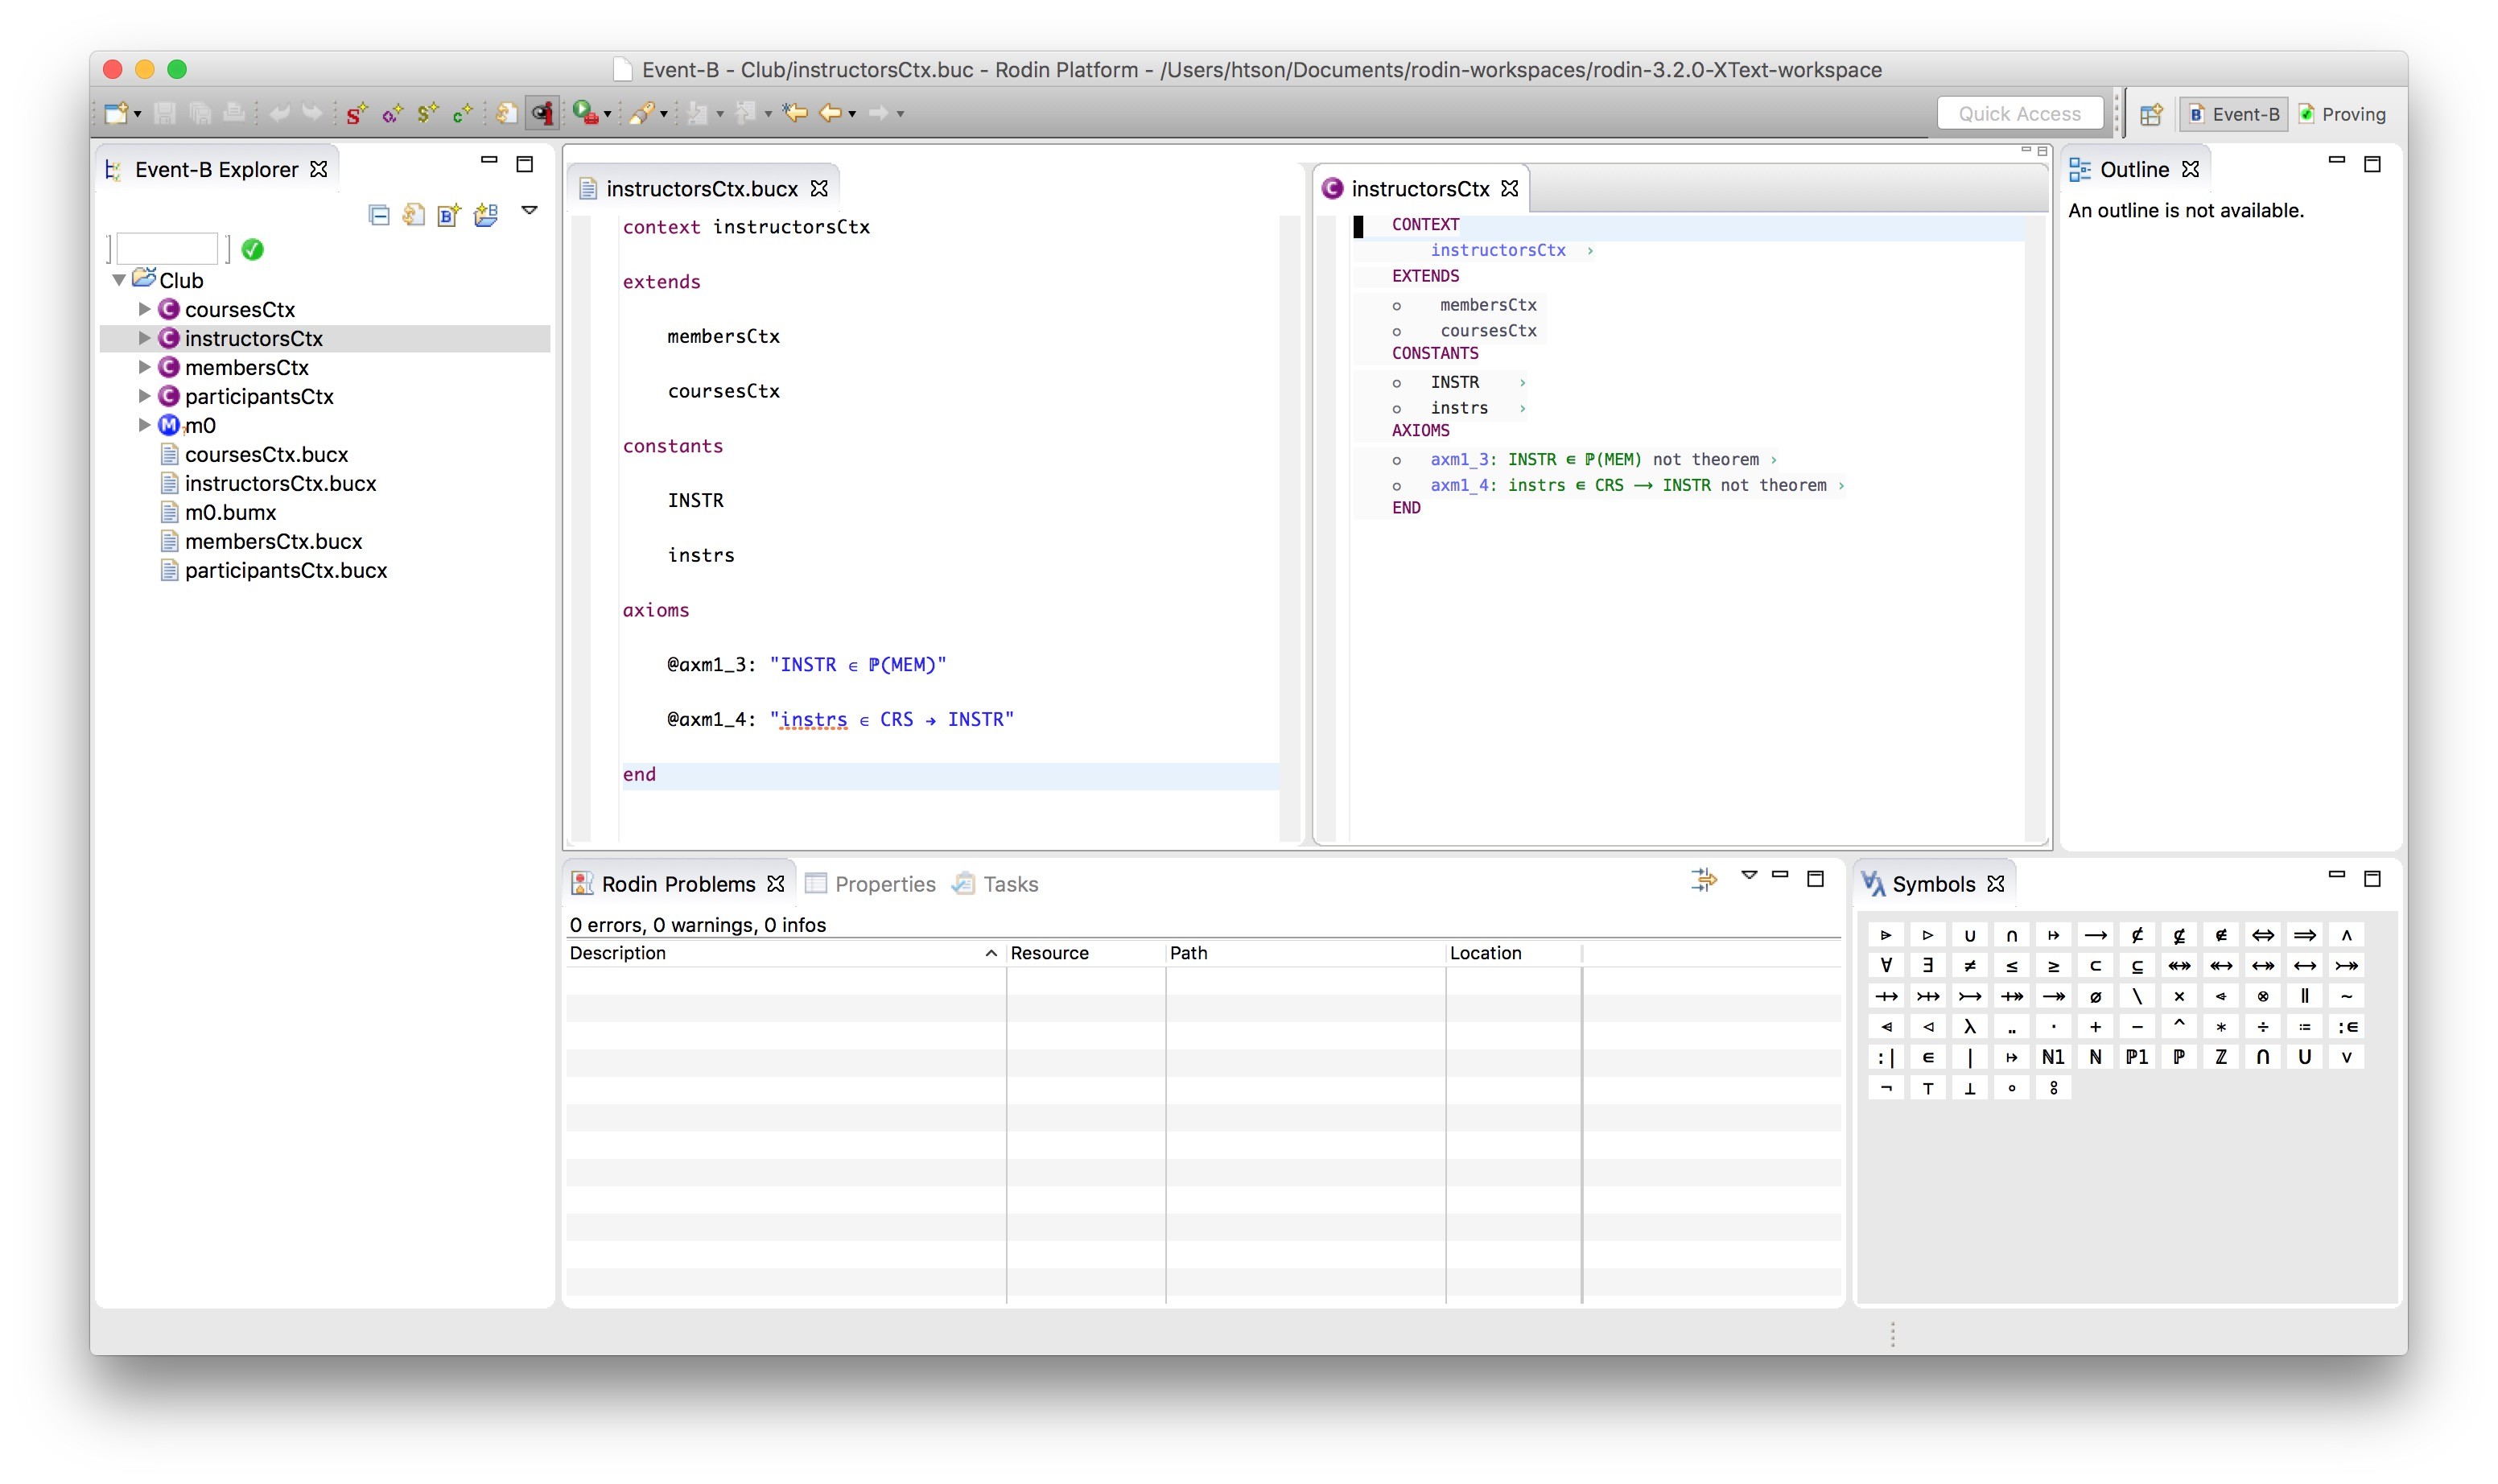
\includegraphics[width=512]{figures/InstructorsCtx}
    \else
    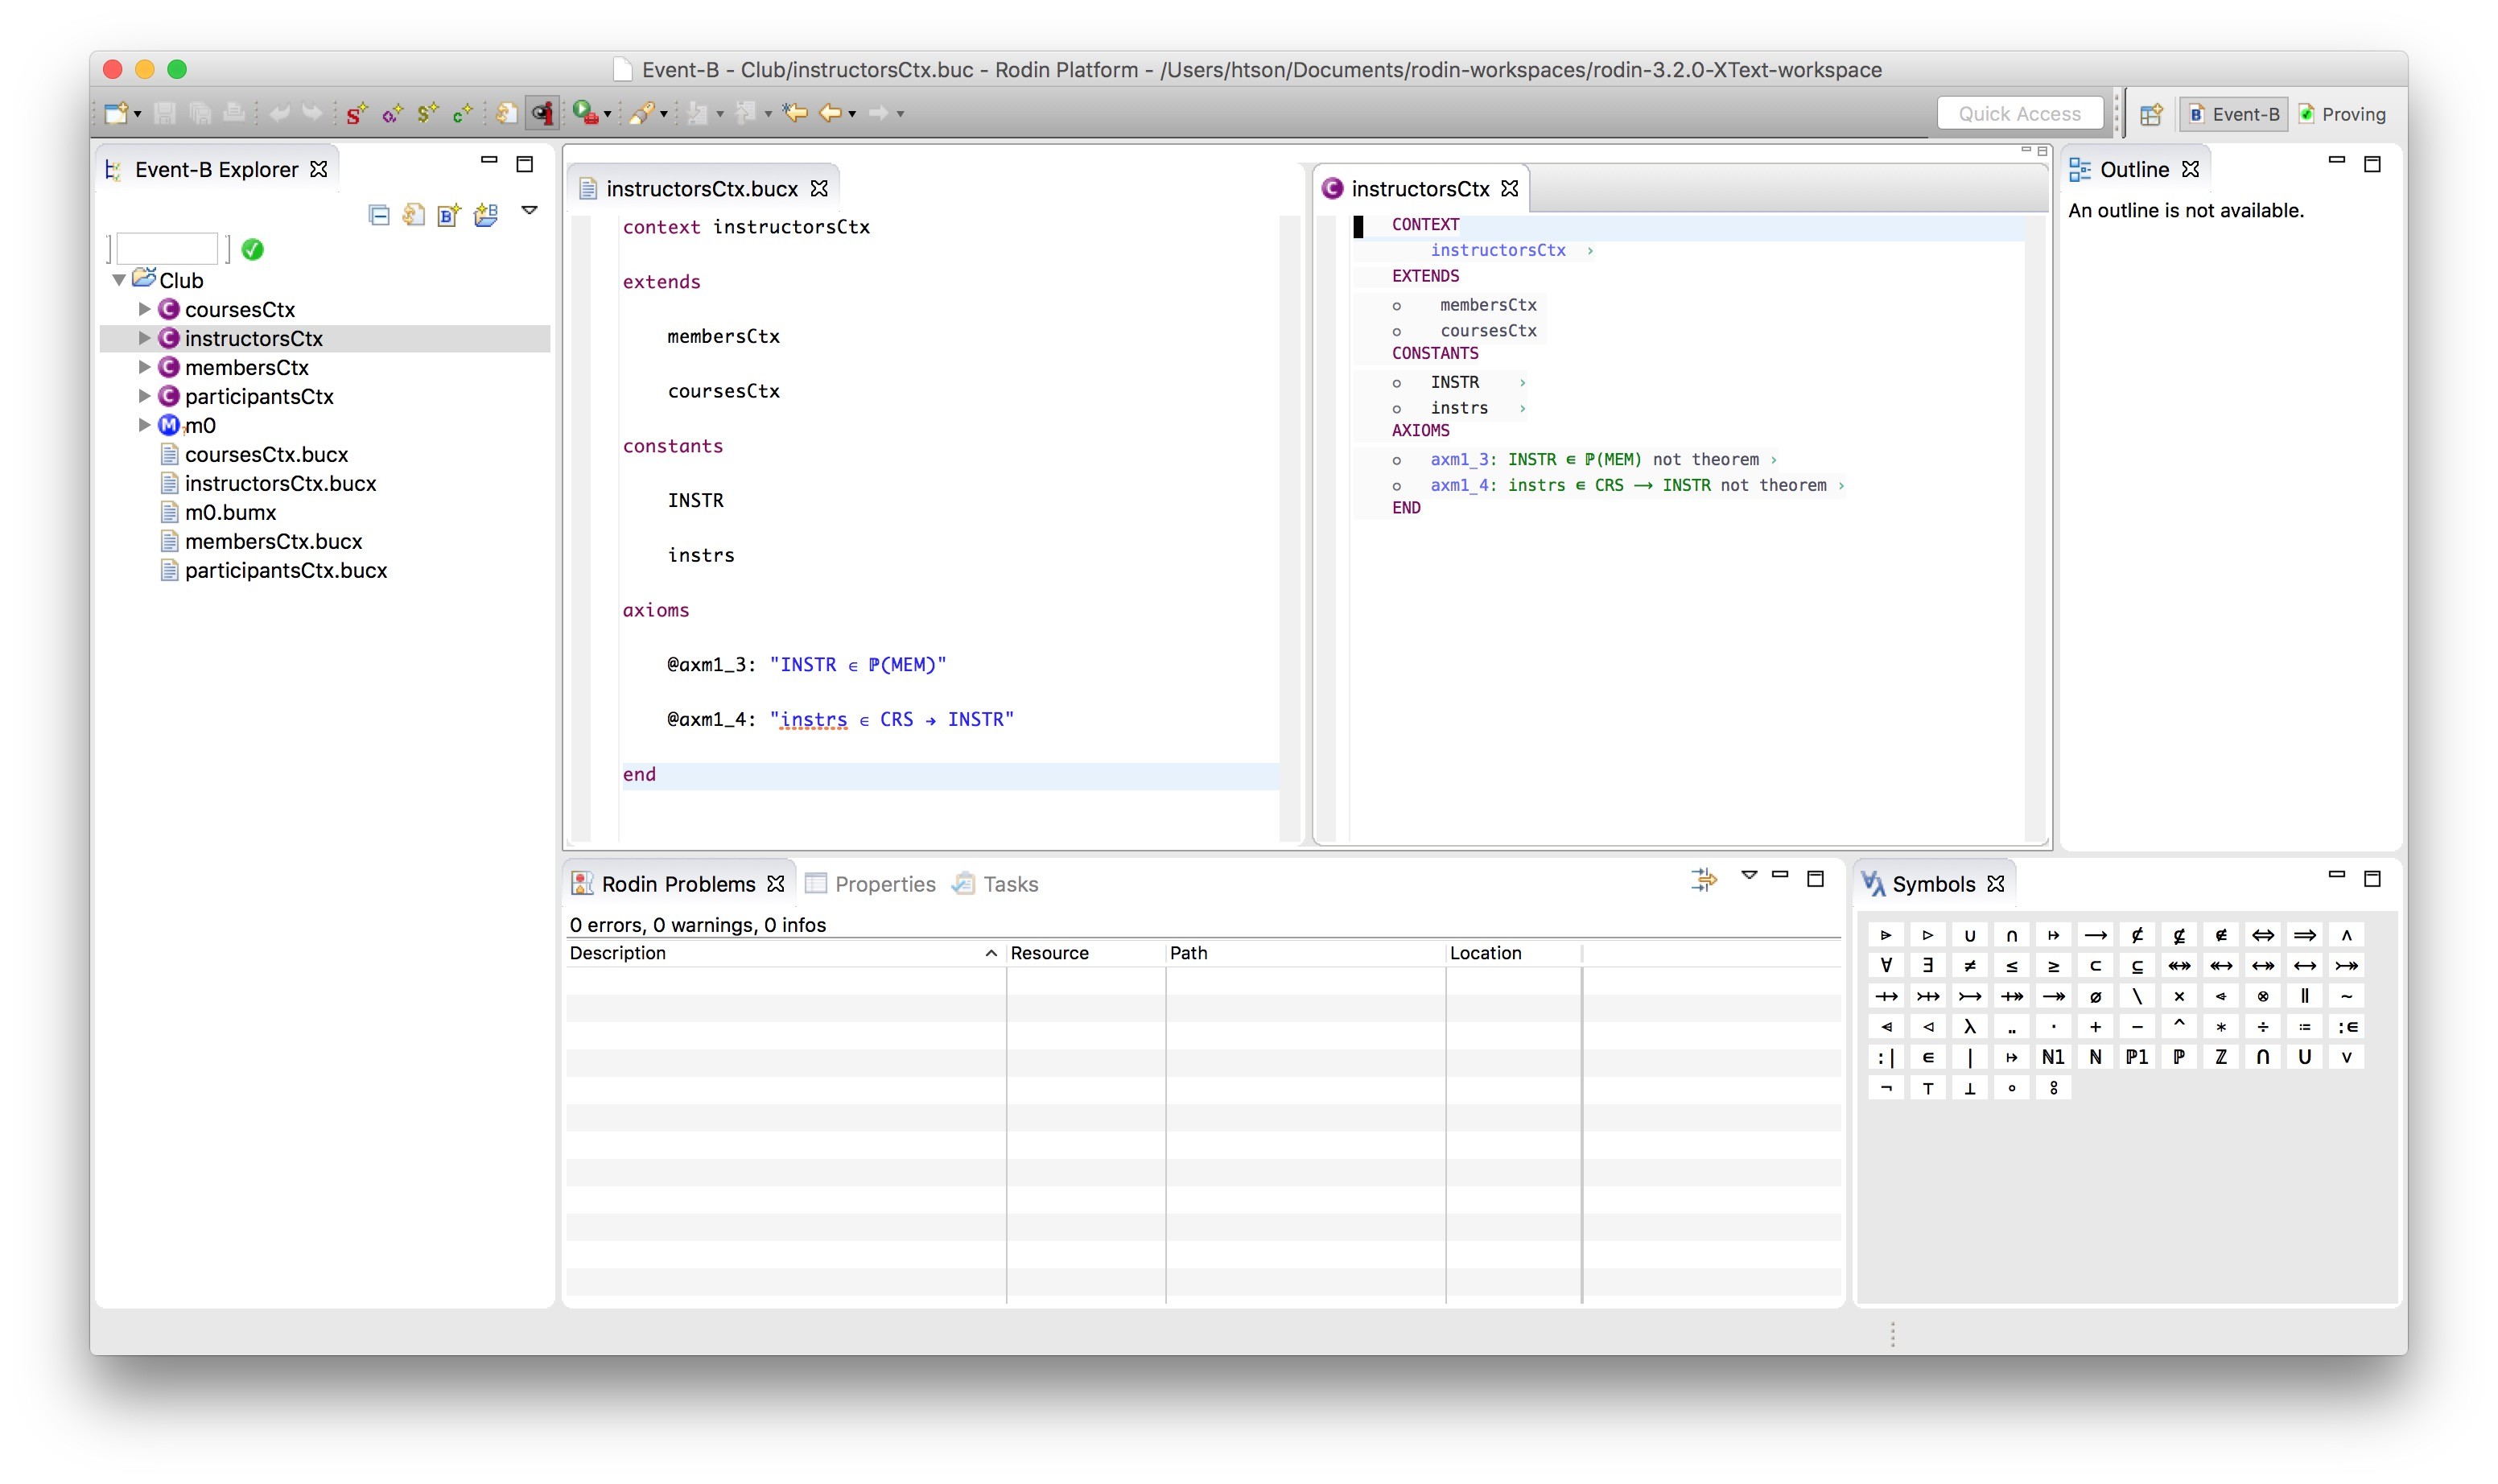
\includegraphics[width=0.9\textwidth]{figures/InstructorsCtx}
    \endif
    \caption{XContext instructorsCtx.bucx}
    \label{fig:instructorsCtx}
  \end{figure}

\subsubsection{Task 6. Create refined XMachines}
\textbf{Introduction} The purpose of this task is to create some more refined XMachines within the ``Club'' project.

\paragraph{Task 6.1. Create a refined XMachine m1.bumx}
\textbf{Introduction} The purpose of this sub-task is to create a refined XMachine ``m1.bumx'' within the ``Club'' project.
\begin{description}
\item[Step 1. Create a new XMachine m1.bumx] \textbf{Create a new XMachine} named ``m1.bumx'' using the \emph{New File wizard} (see Figure~\ref{fig:CreateM1}. The newly created file should be opened automatically in an XMachine editor.
  \begin{figure}[!htbp]
    \centering
    \ifdef{PLASTEX}
    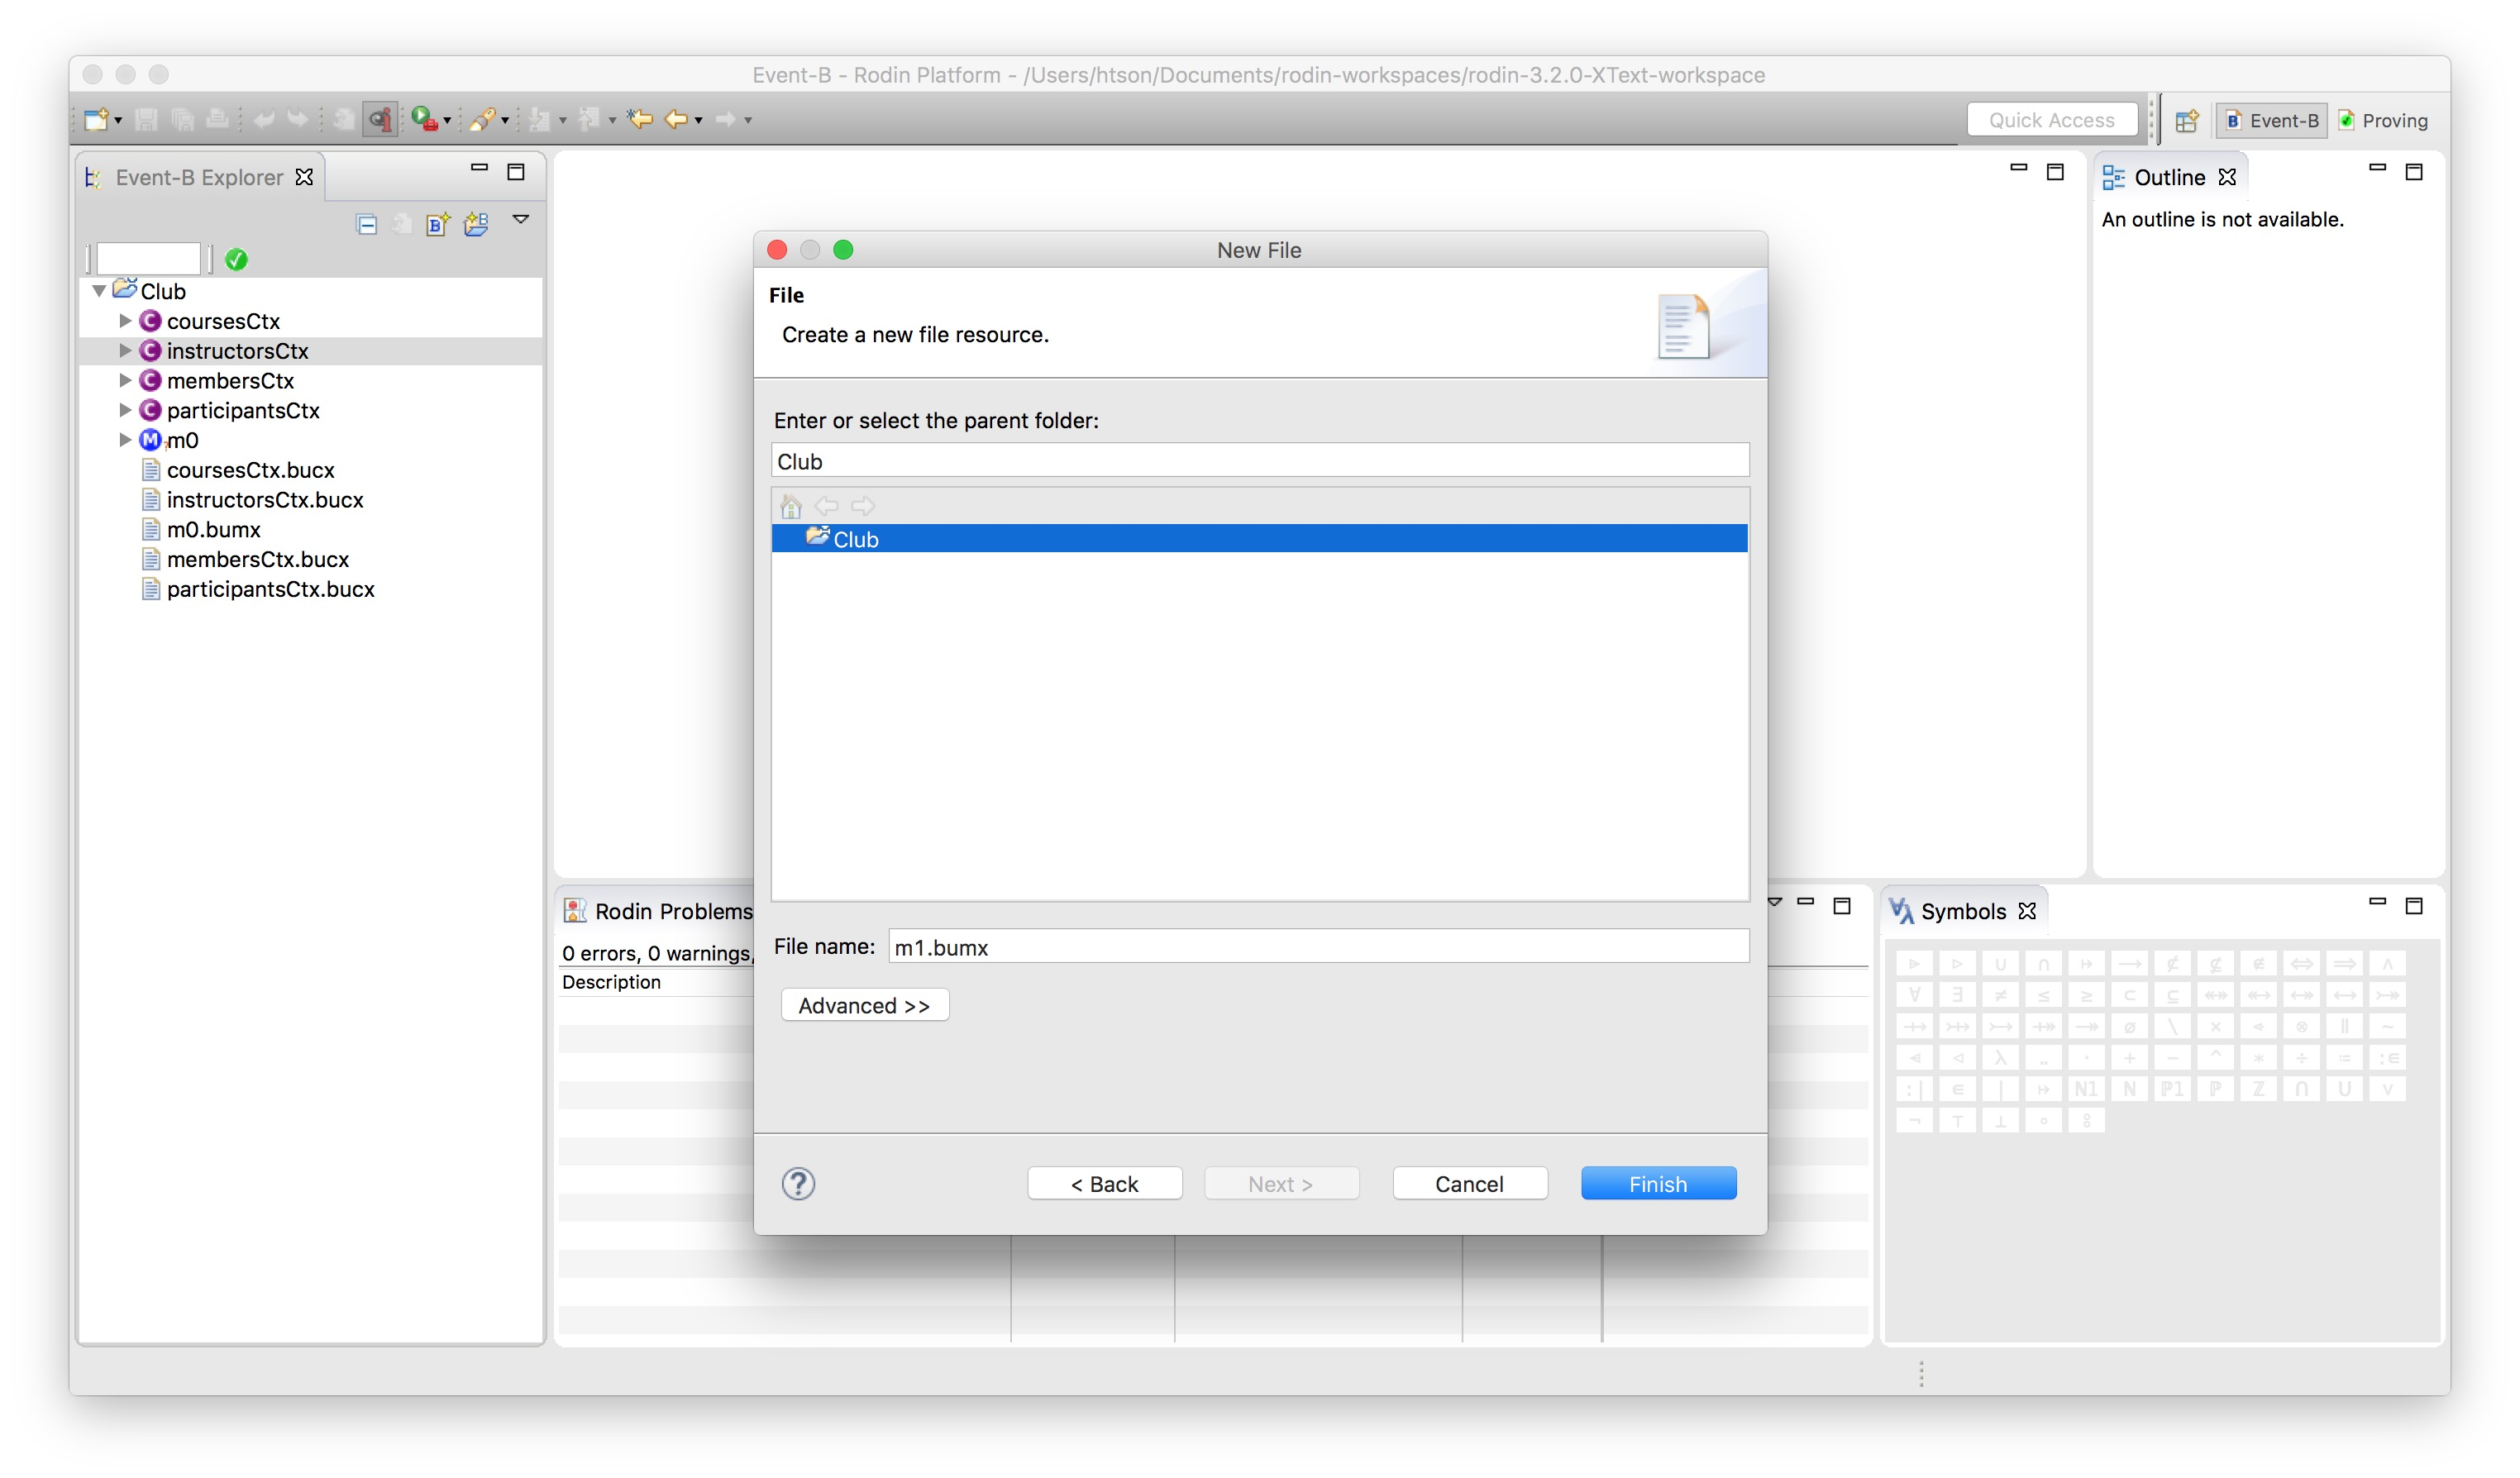
\includegraphics[width=512]{figures/CreateM1}
    \else
    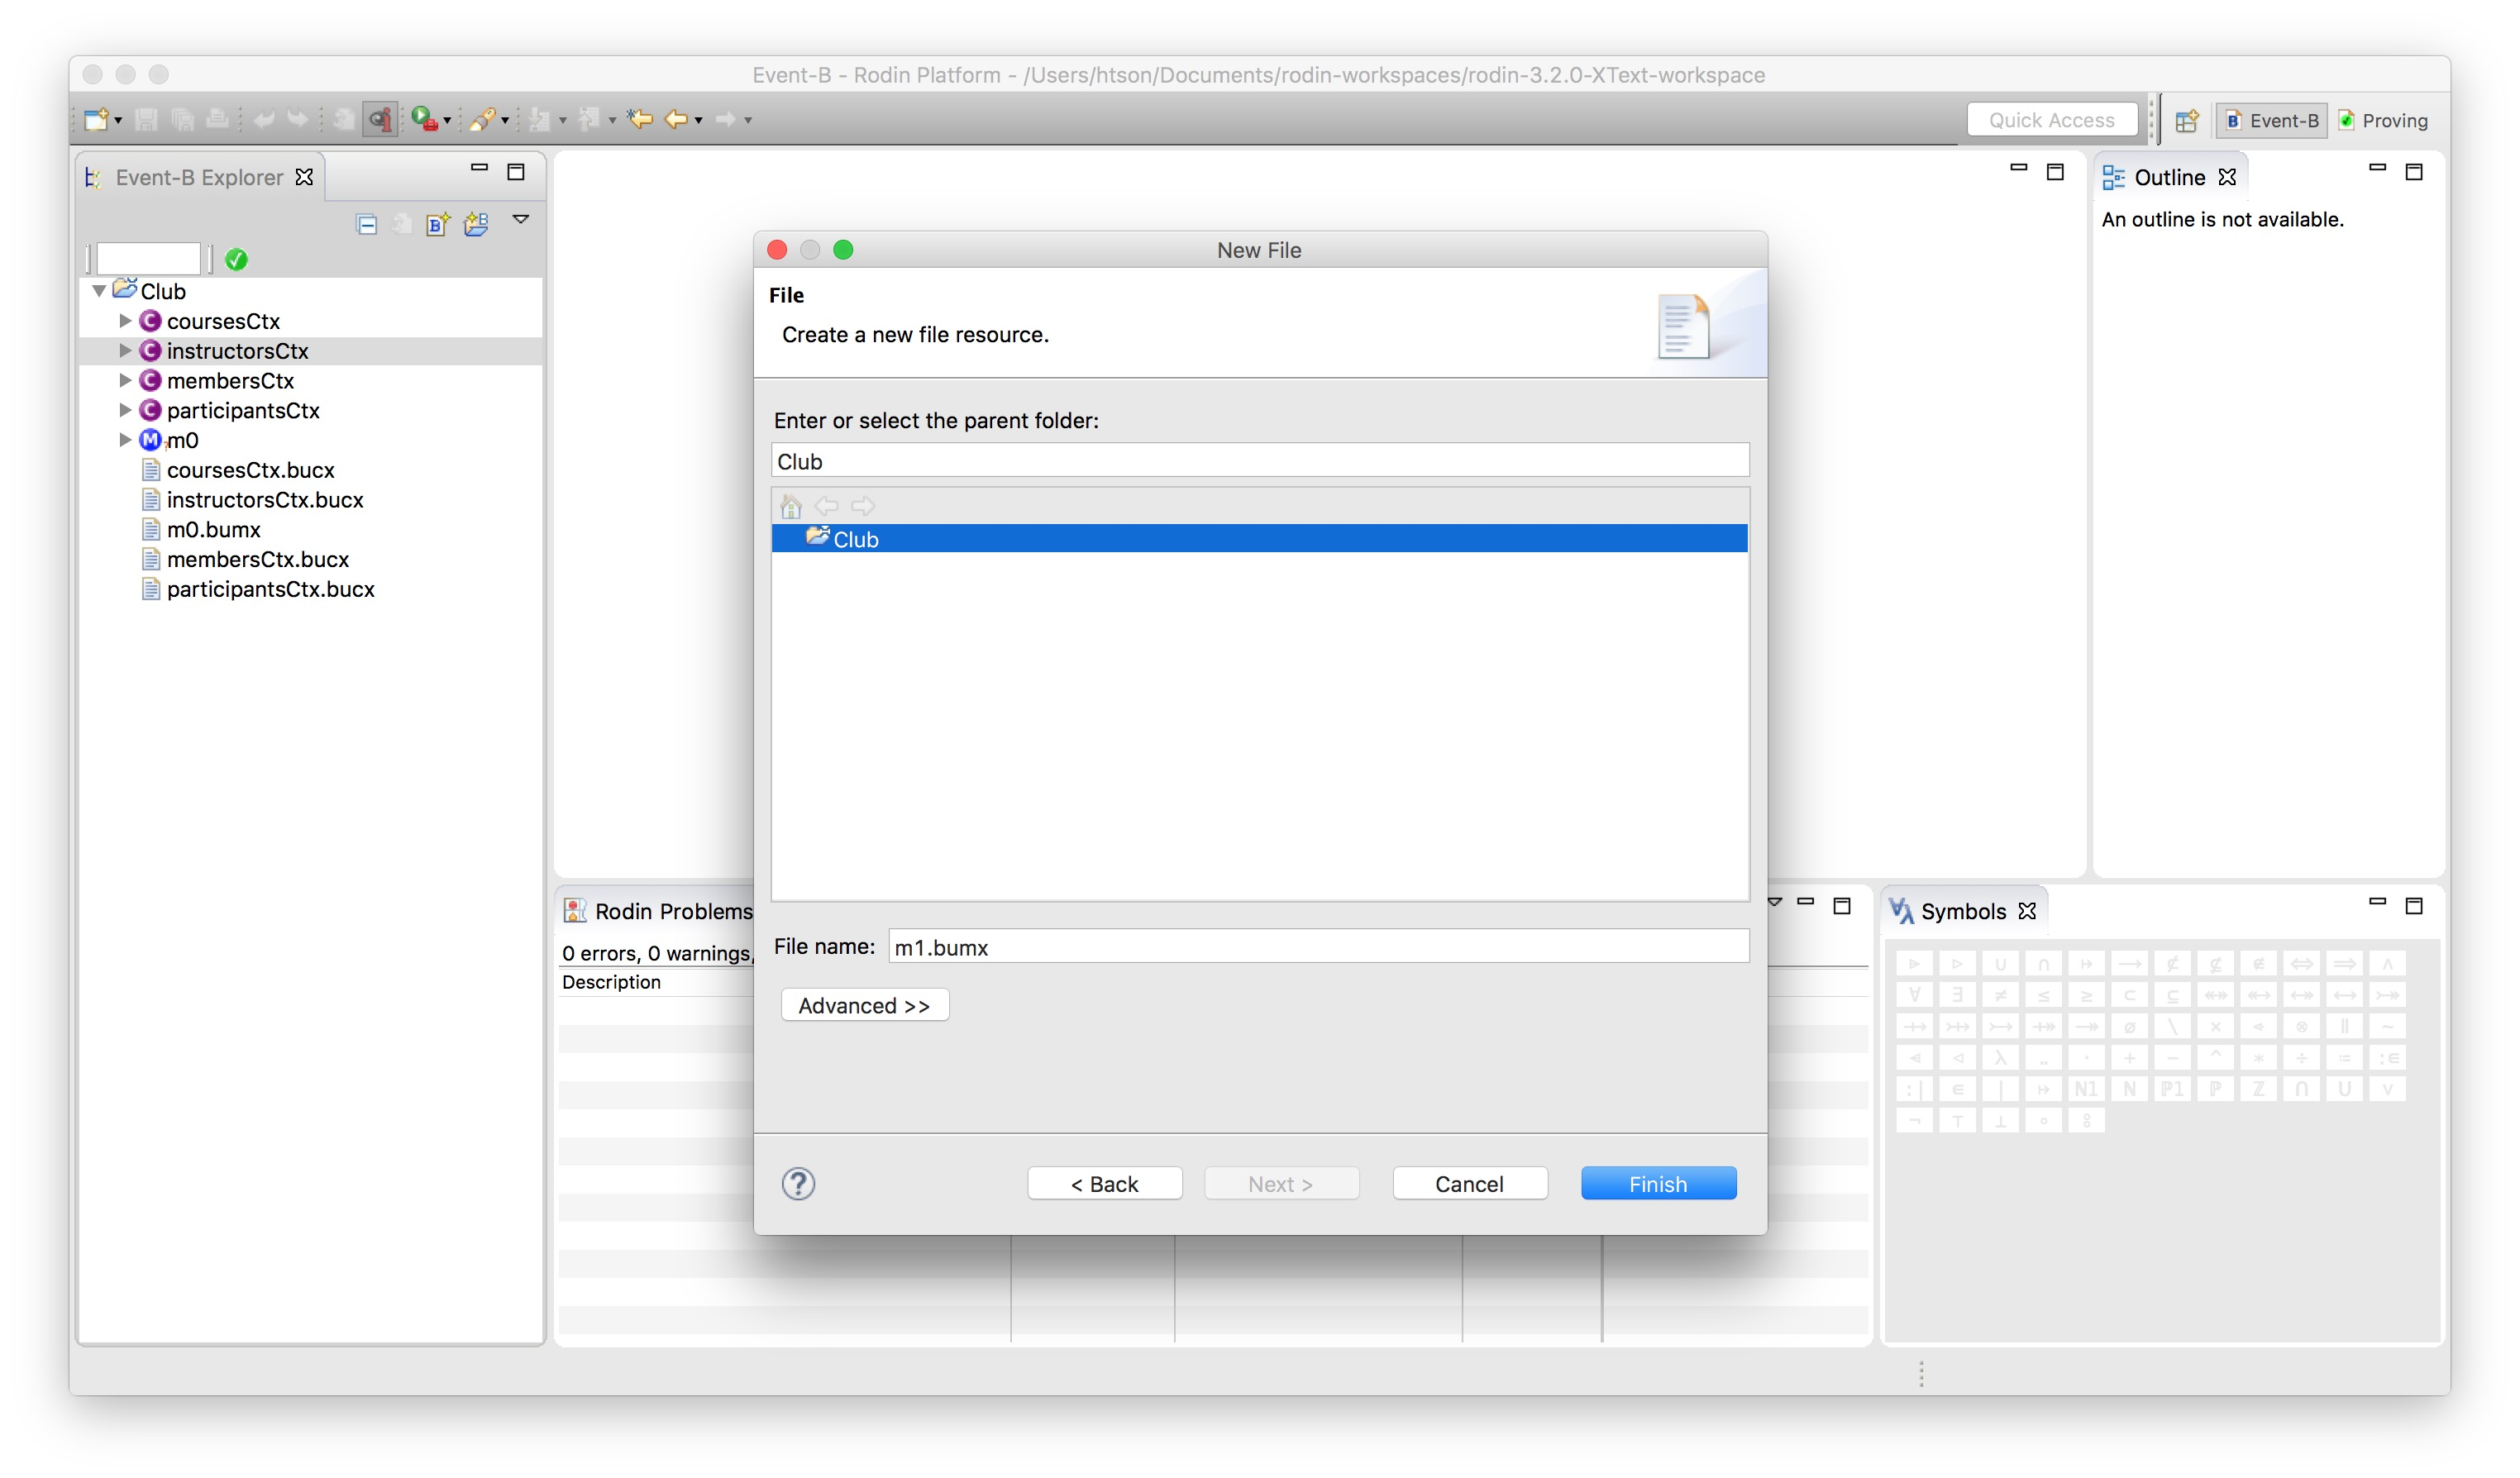
\includegraphics[width=0.9\textwidth]{figures/CreateM1}
    \endif
    \caption{Create m1.bumx}
    \label{fig:CreateM1}
  \end{figure}

\item[Step 2. Set the content of m1.bumx] \textbf{Set the content of ``m1.bumx'' as follows}.
  \begin{center}
    \begin{Bcode}
      \ifdef{PLASTEX}
      \Bmachine{} m1\\
      \Brefines{} m0\\
      \Bsees{} instructorsCtx participantsCtx \\
      \Bvariables{} crs prtcpts \\
      \Binvariants\\
      @inv1_1: prtcpts ∈ crs ↔ PRTCPT\\
      @inv1_2: ∀c·c ∈ crs ⇒ instrs(c) ∉ prtcpts[\{c\}]\\
      variants @v0: (crs × PRTCPT) ∖ prtcpts\\
      \Bevents\\
      event INITIALISATION extends INITIALISATION\\
      \Bthen\\
      @act1_2: prtcpts ≔ ∅\\
      \Bend\\
      event OpenCourses \Brefines{} OpenCourses\\
      \Bwhere\\
      \Btheorem{} @thm1_2: dom(prtcpts) ⊆ crs\\
      \Bend\\
      \Banticipated{} event CloseCourses extends CloseCourses\\
      \Bthen\\
      @act1_2: prtcpts ≔ cs ⩤ prtcpts\\
      \Bend\\
      \Bconvergent event Register \\
      \Bany{} p c \Bwhere \\
      @grd1_1: p ∈ PRTCPT\\
      @grd1_2: c ∈ crs\\
      @grd1_3: p ≠ instrs(c)\\
      @grd1_4: c ↦ p ∉ prtcpts\\
      \Bthen\\
      @act1_1: prtcpts ≔ prtcpts ∪ \{c ↦ p\}\\
      \Bend\\
      \Bend
      \else
      \Bmachine{} m1\\
      \Brefines{} m0\\
      \Bsees{} instructorsCtx participantsCtx \\
      \Bvariables{} crs prtcpts \\
      \Binvariants\\
      \Btab @inv1_1: \(prtcpts \in crs \rel PRTCPT\)\\
      \Btab @inv1_2: \(\forall c \qdot c ∈ crs \limp instrs(c) \notin prtcpts[\{c\}]\)\\
      variants @v0:\((crs \cprod PRTCPT) \setminus prtcpts\)\\
      \Bevents\\
      \Btab event INITIALISATION extends INITIALISATION\\
      \Btab \Bthen\\
      \Btab \Btab @act1_2: \(prtcpts \bcmeq \emptyset\)\\
      \Btab \Bend\\
      \Btab event OpenCourses extends OpenCourses\\
      \Btab \Bwhere\\
      \Btab \Btab \Btheorem{} @thm1_2: \(\dom(prtcpts) \subseteq crs\) \\
      \Btab \Bend\\
      \Btab \Banticipated{} event CloseCourses extends CloseCourses\\
      \Btab \Bthen\\
      \Btab \Btab @act1_2: \(prtcpts \bcmeq cs \domsub prtcpts\)\\
      \Btab \Bend\\
      \Btab \Bconvergent{} event Register \\
      \Btab \Bany{} p c \Bwhere \\
      \Btab \Btab @grd1_1: \(p \in PRTCPT\)\\
      \Btab \Btab @grd1_2: \(c \in crs\)\\
      \Btab \Btab @grd1_3: \(p \neq instrs(c)\)\\
      \Btab \Btab @grd1_4: \(c \mapsto p \neq prtcpts\)\\
      \Btab \Bthen\\
      \Btab \Btab @act1_1: \(prtcpts \bcmeq prtcpts \bunion \{c \mapsto p\}\)\\
      \Btab \Bend\\
      \Bend
      \endif
    \end{Bcode}
  \end{center}

\item[Step 3. Auto-format the code] \textbf{Automatically format the content of ``m1.bumx''} by using short-cut (e.g., on Mac OS: Cmd+Shift+F).

\item[Step 4. Save the file] Save the file ``m1.bumx''.
\end{description}

\textbf{Conclusion} By now, the XMachine ``m1.bucx'' and the corresponding Rodin Machine ``m1'' should be visible in the Event-B Explorer (see Figure~\ref{fig:M1}).
  \begin{figure}[!htbp]
    \centering
    \ifdef{PLASTEX}
    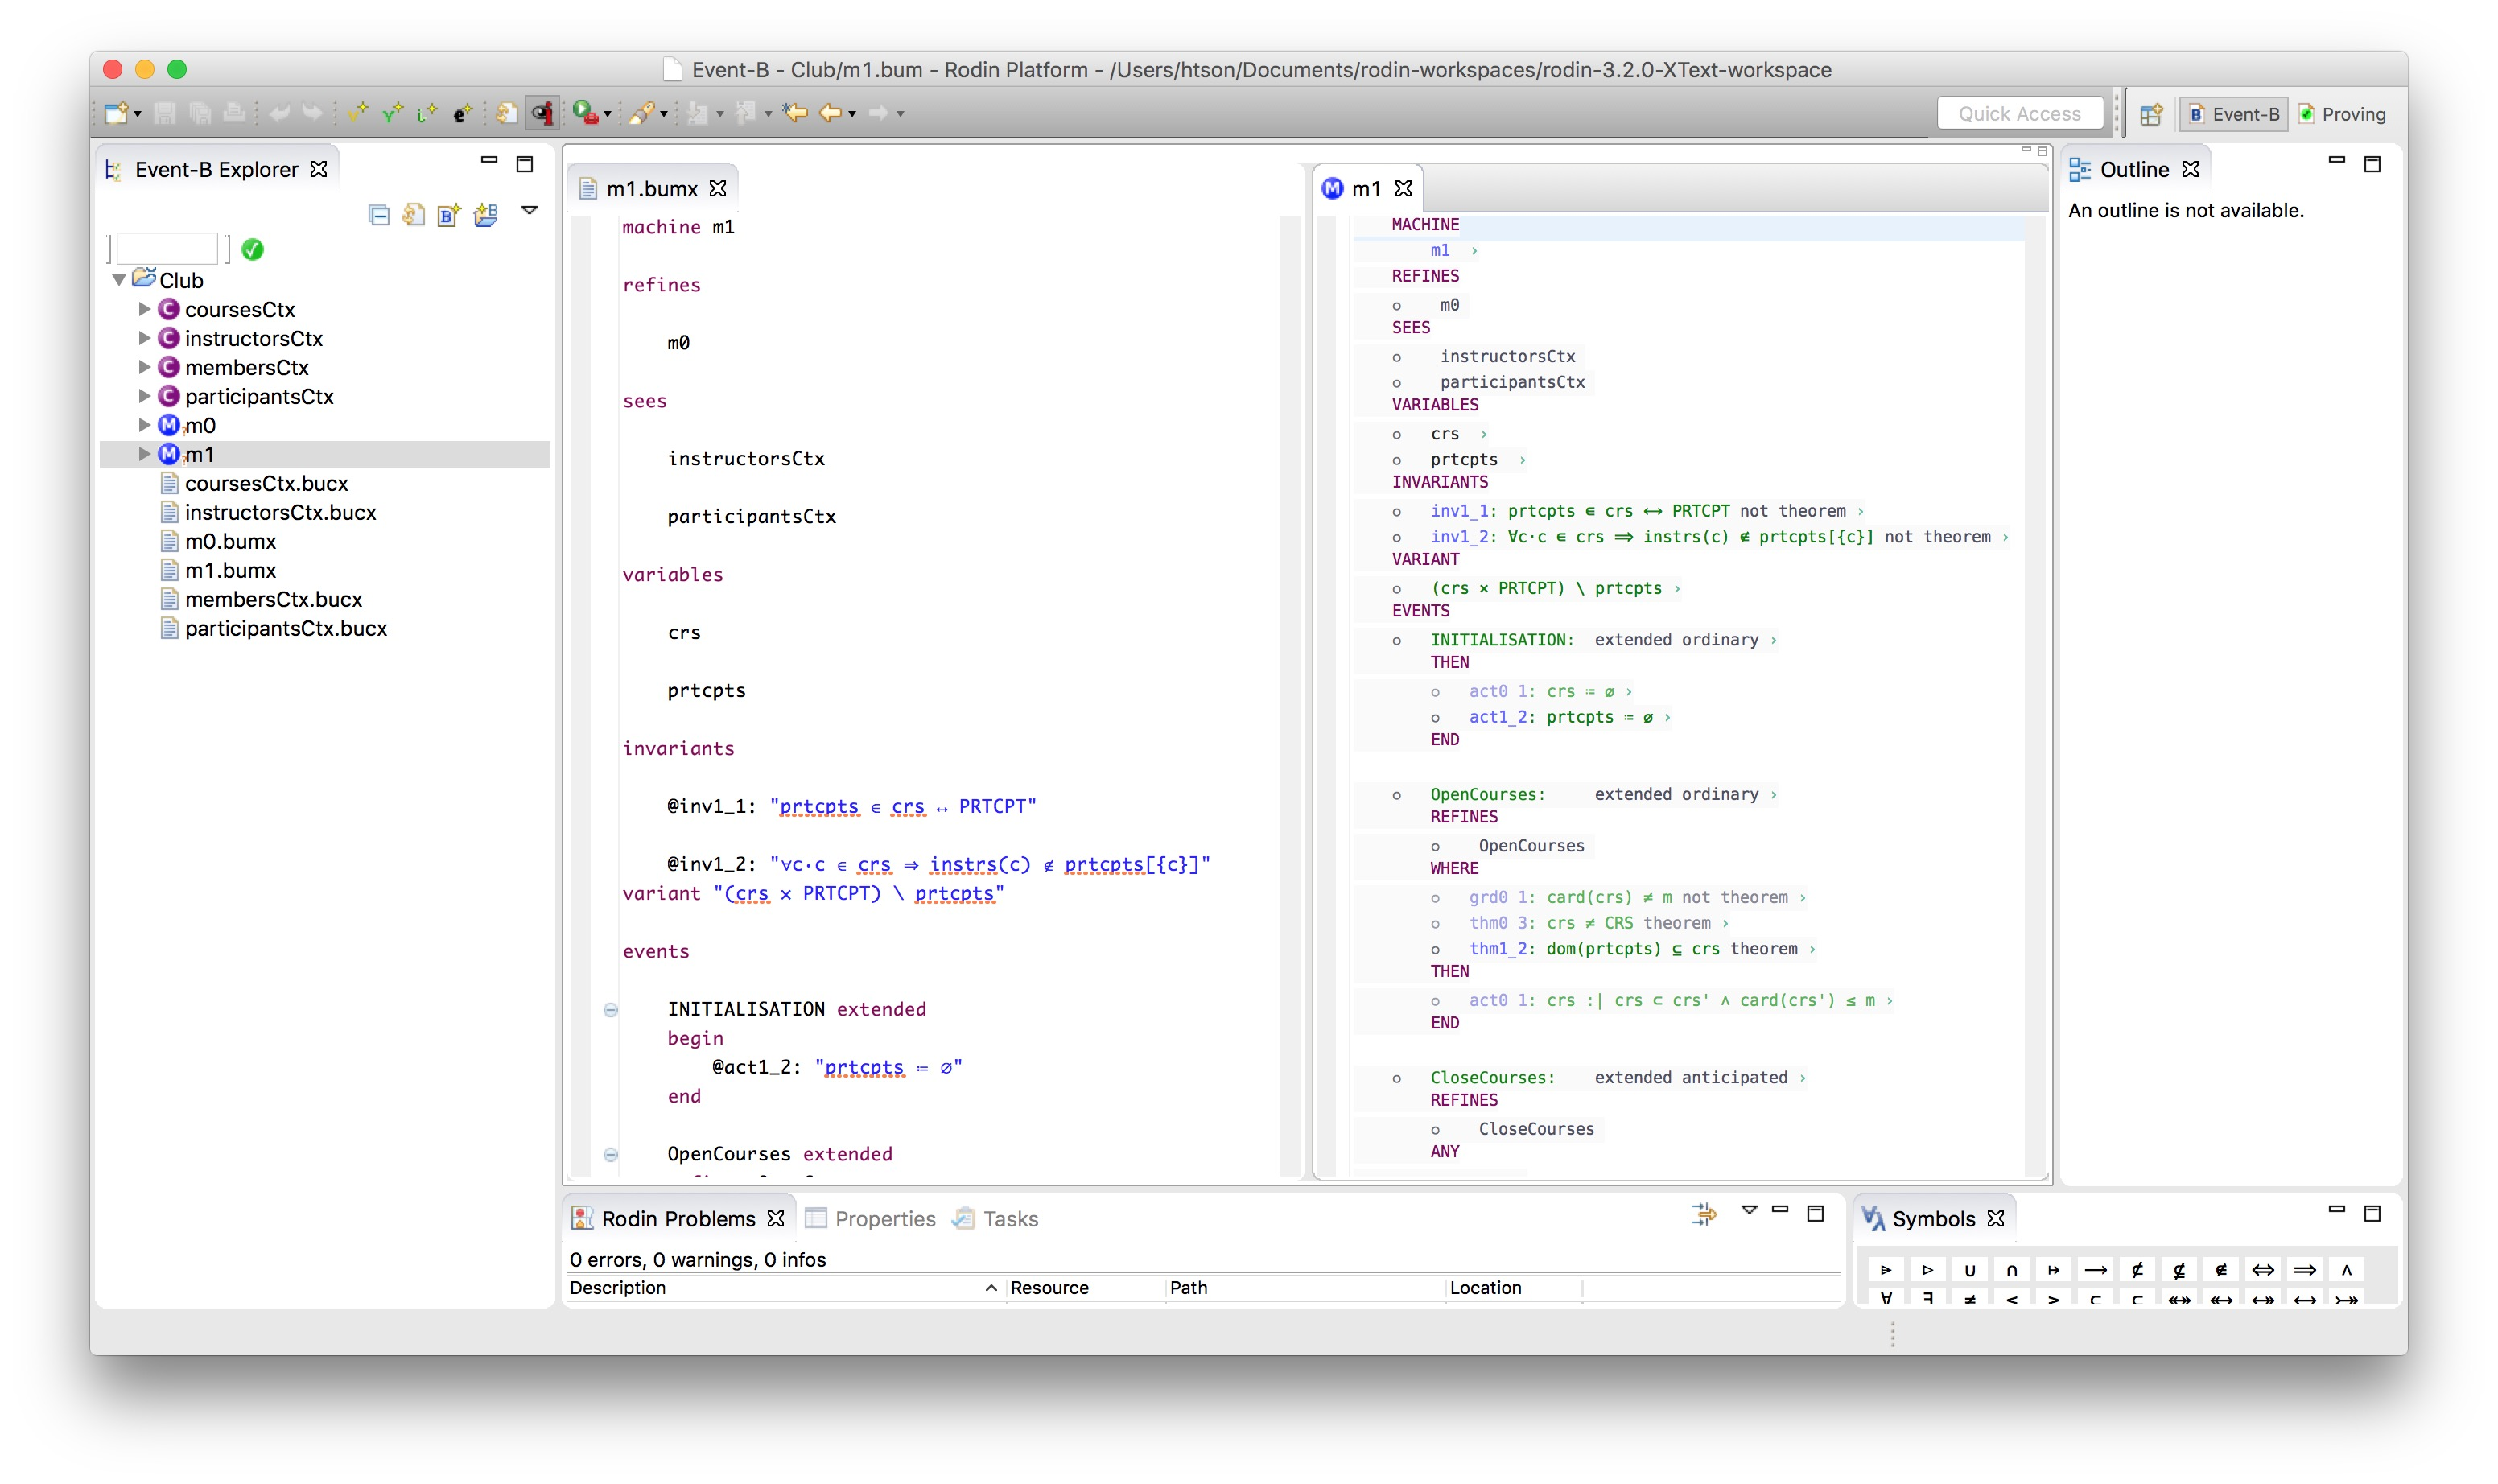
\includegraphics[width=512]{figures/M1}
    \else
    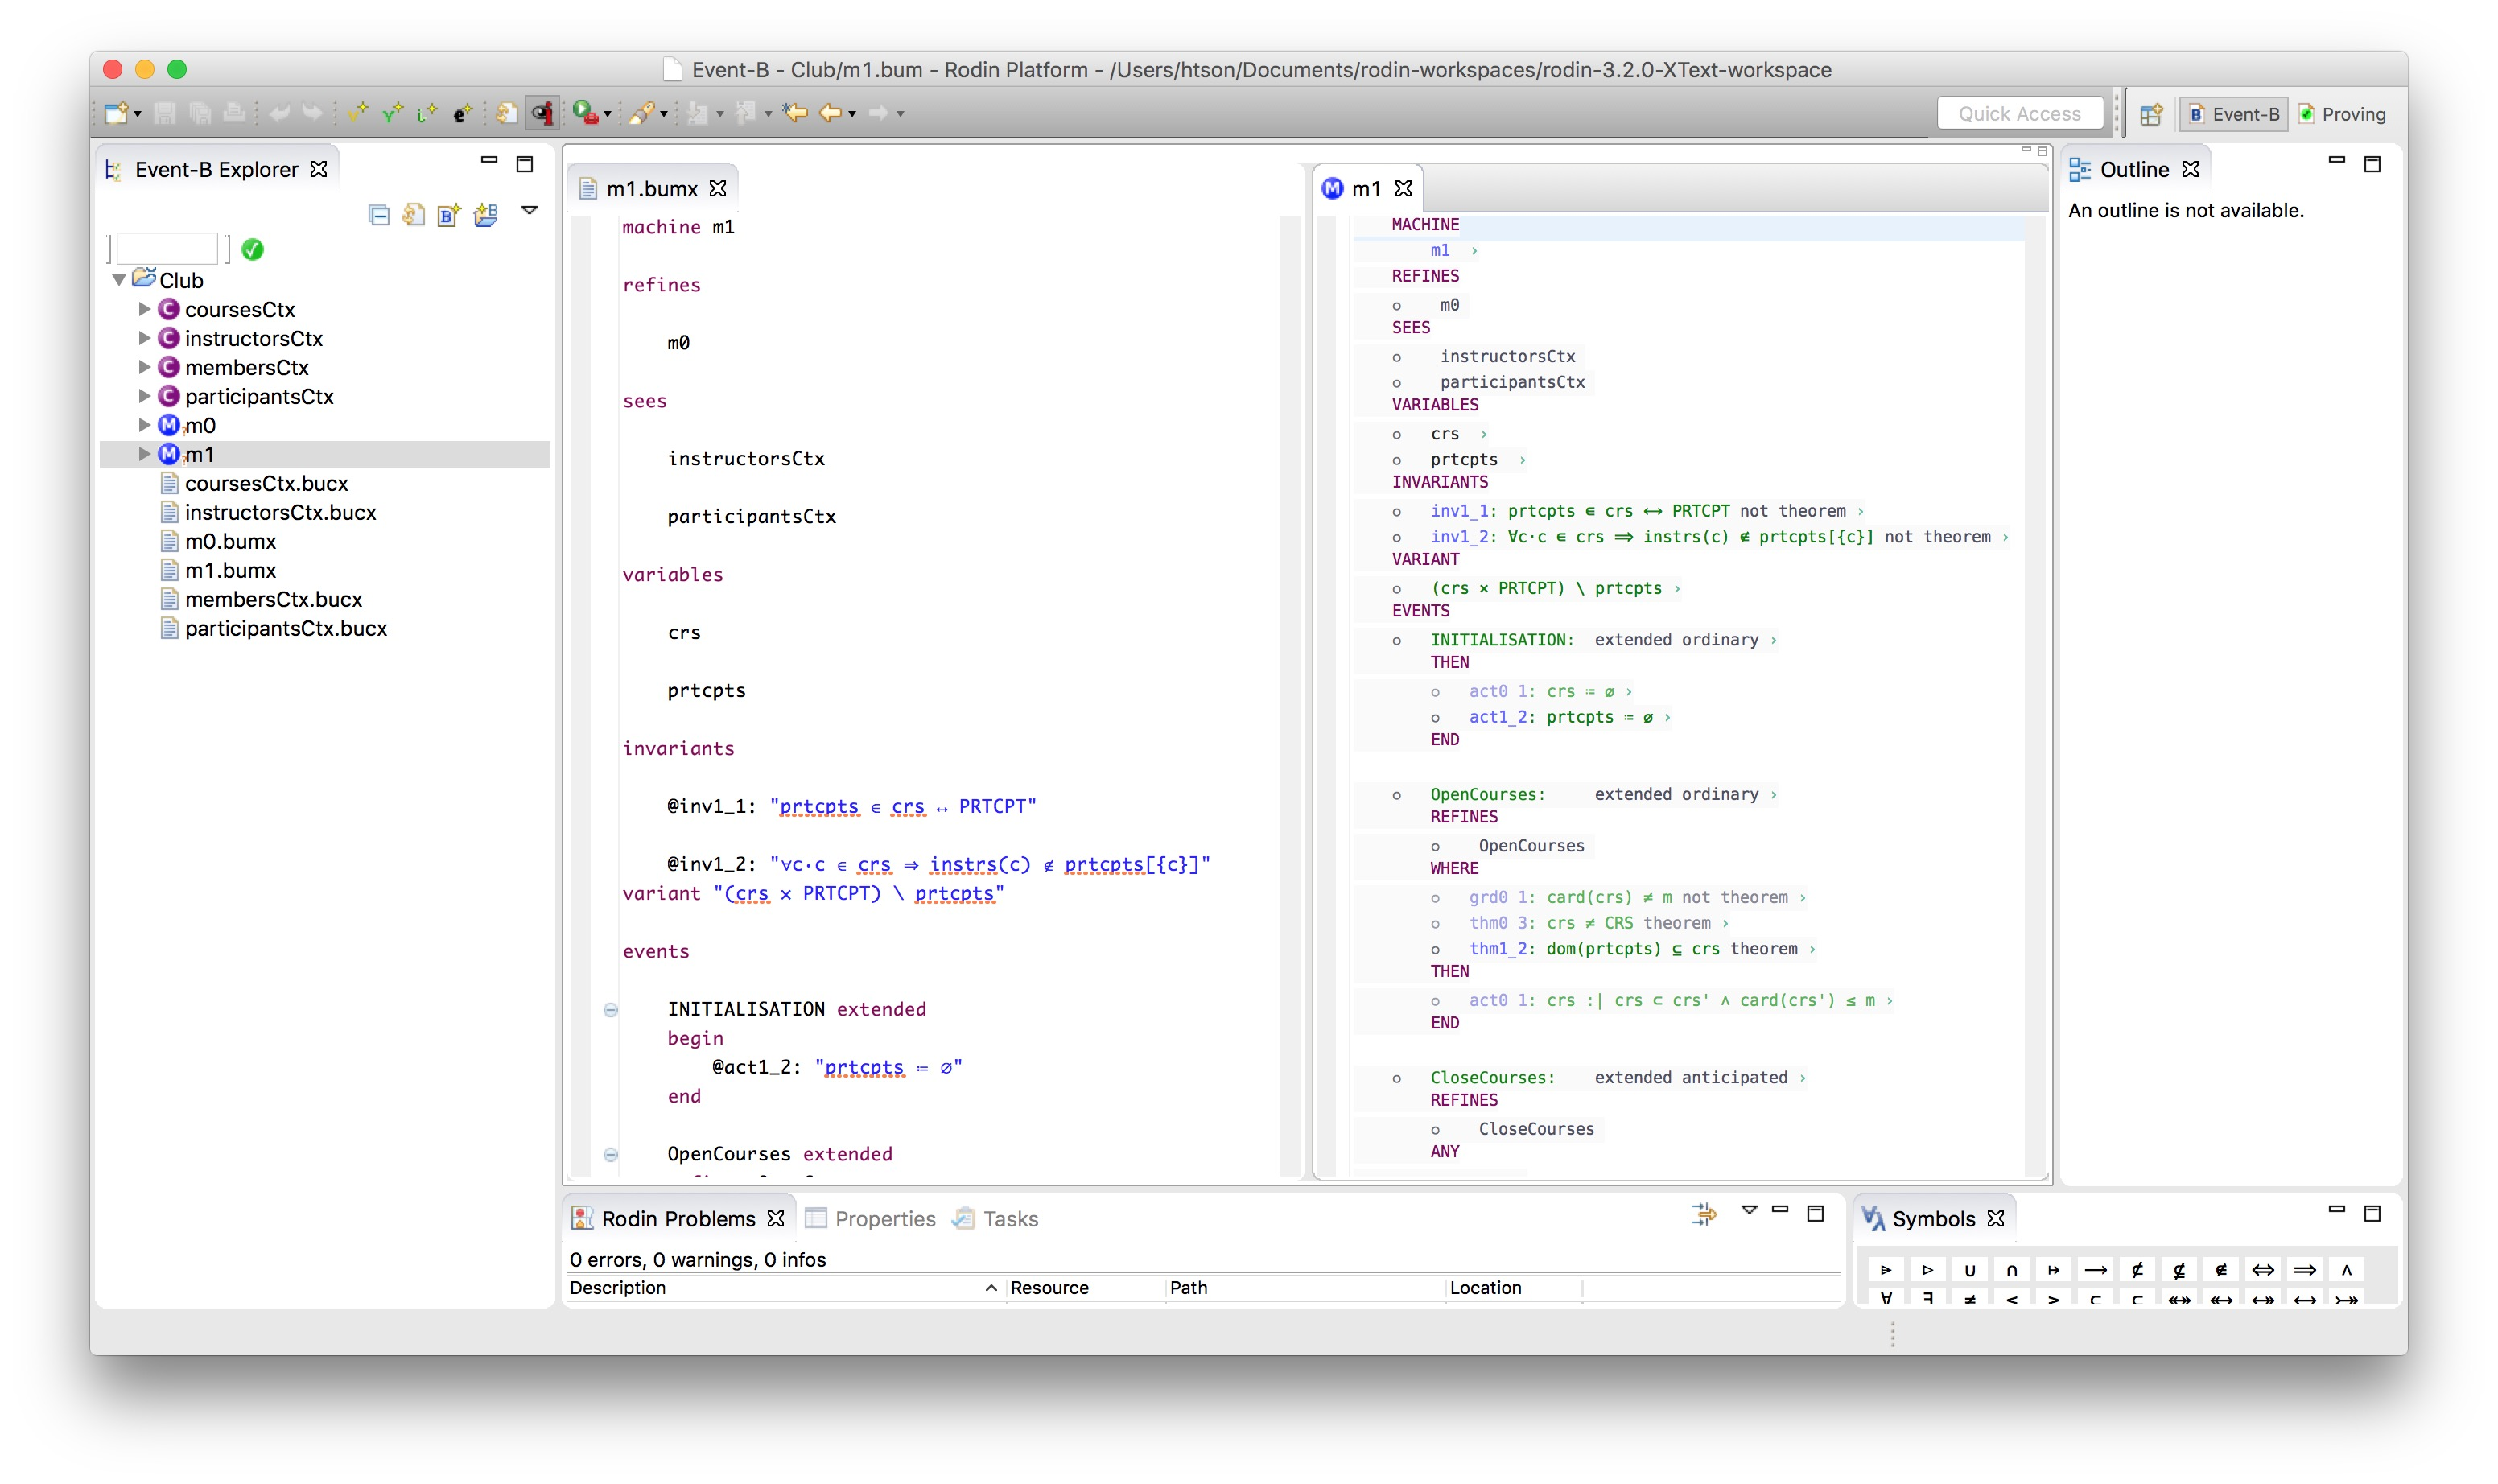
\includegraphics[width=0.9\textwidth]{figures/M1}
    \endif
    \caption{XMachine m1.bumx}
    \label{fig:M1}
  \end{figure}

\paragraph{Task 6.2. Create a refined XMachine m2.bumx}
\textbf{Introduction} The purpose of this sub-task is to create a refined XMachine ``m2.bumx'' within the ``Club'' project.

\begin{description}
\item[Step 1. Create a new XMachine m2.bumx] \textbf{Create a new XMachine} named ``m2.bumx'' using the \emph{New File wizard} (see Figure~\ref{fig:CreateM2}. The newly created file should be opened automatically in an XMachine editor.
  \begin{figure}[!htbp]
    \centering
    \ifdef{PLASTEX}
    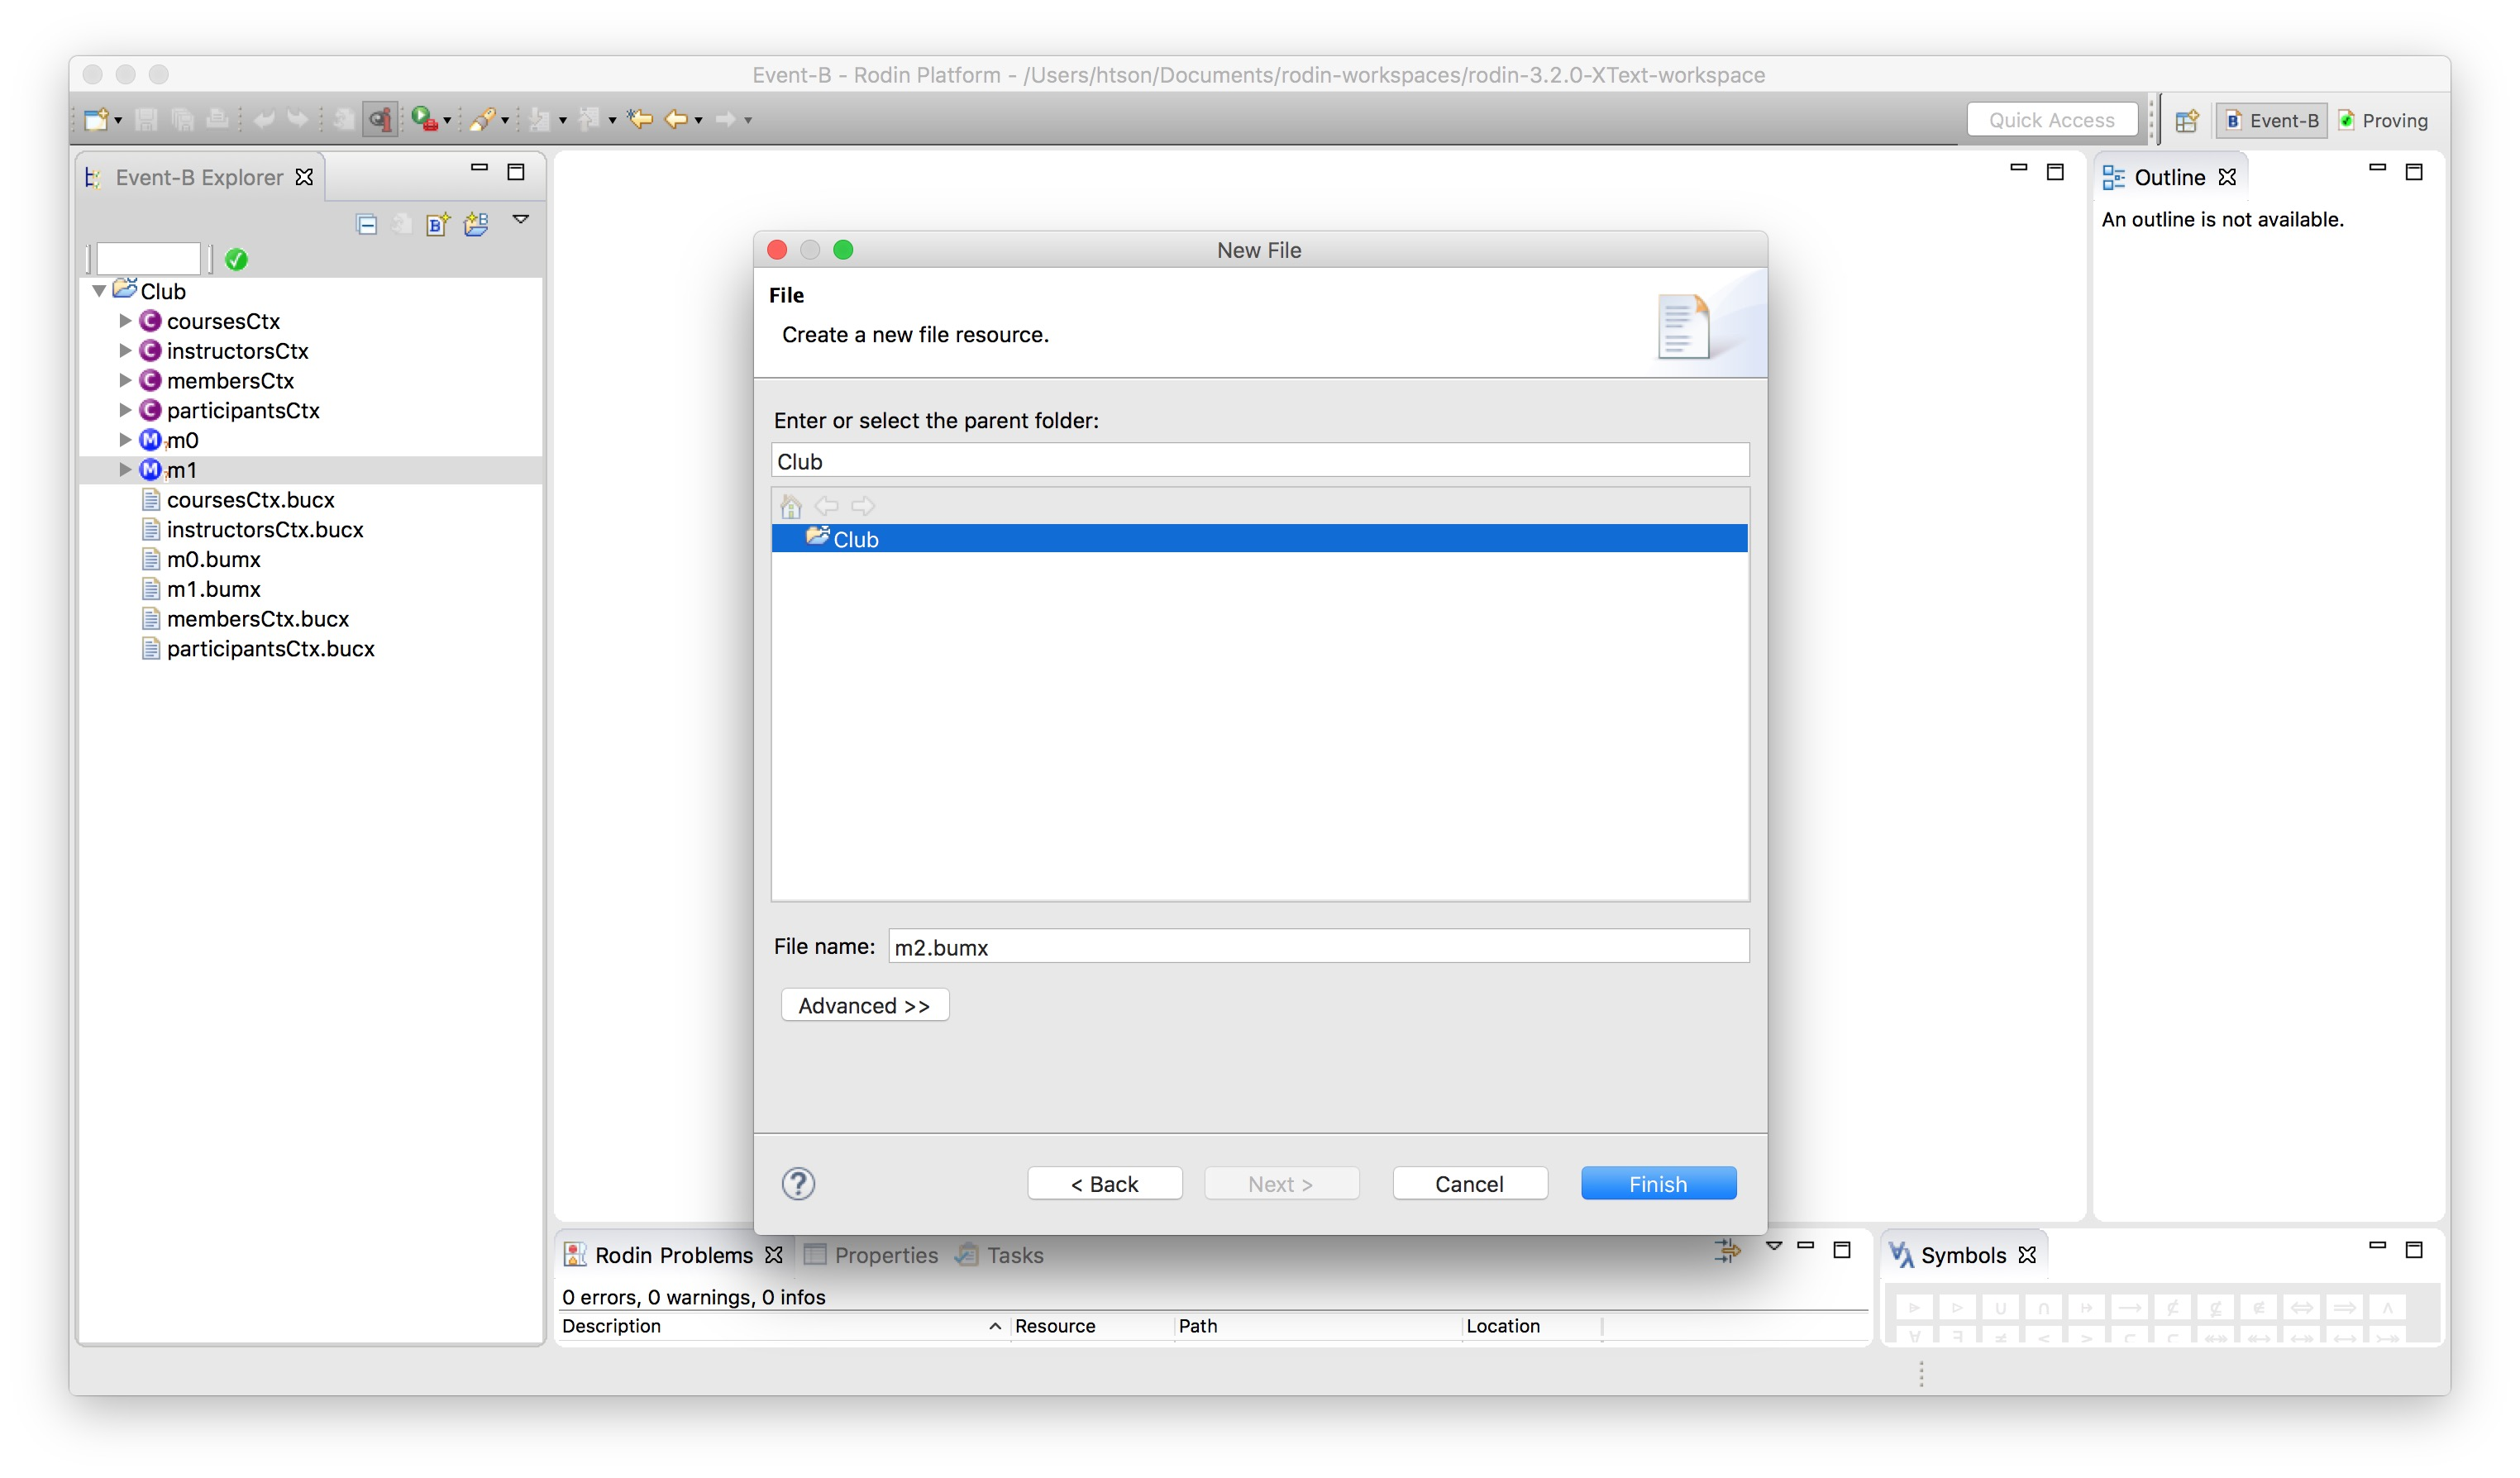
\includegraphics[width=512]{figures/CreateM2}
    \else
    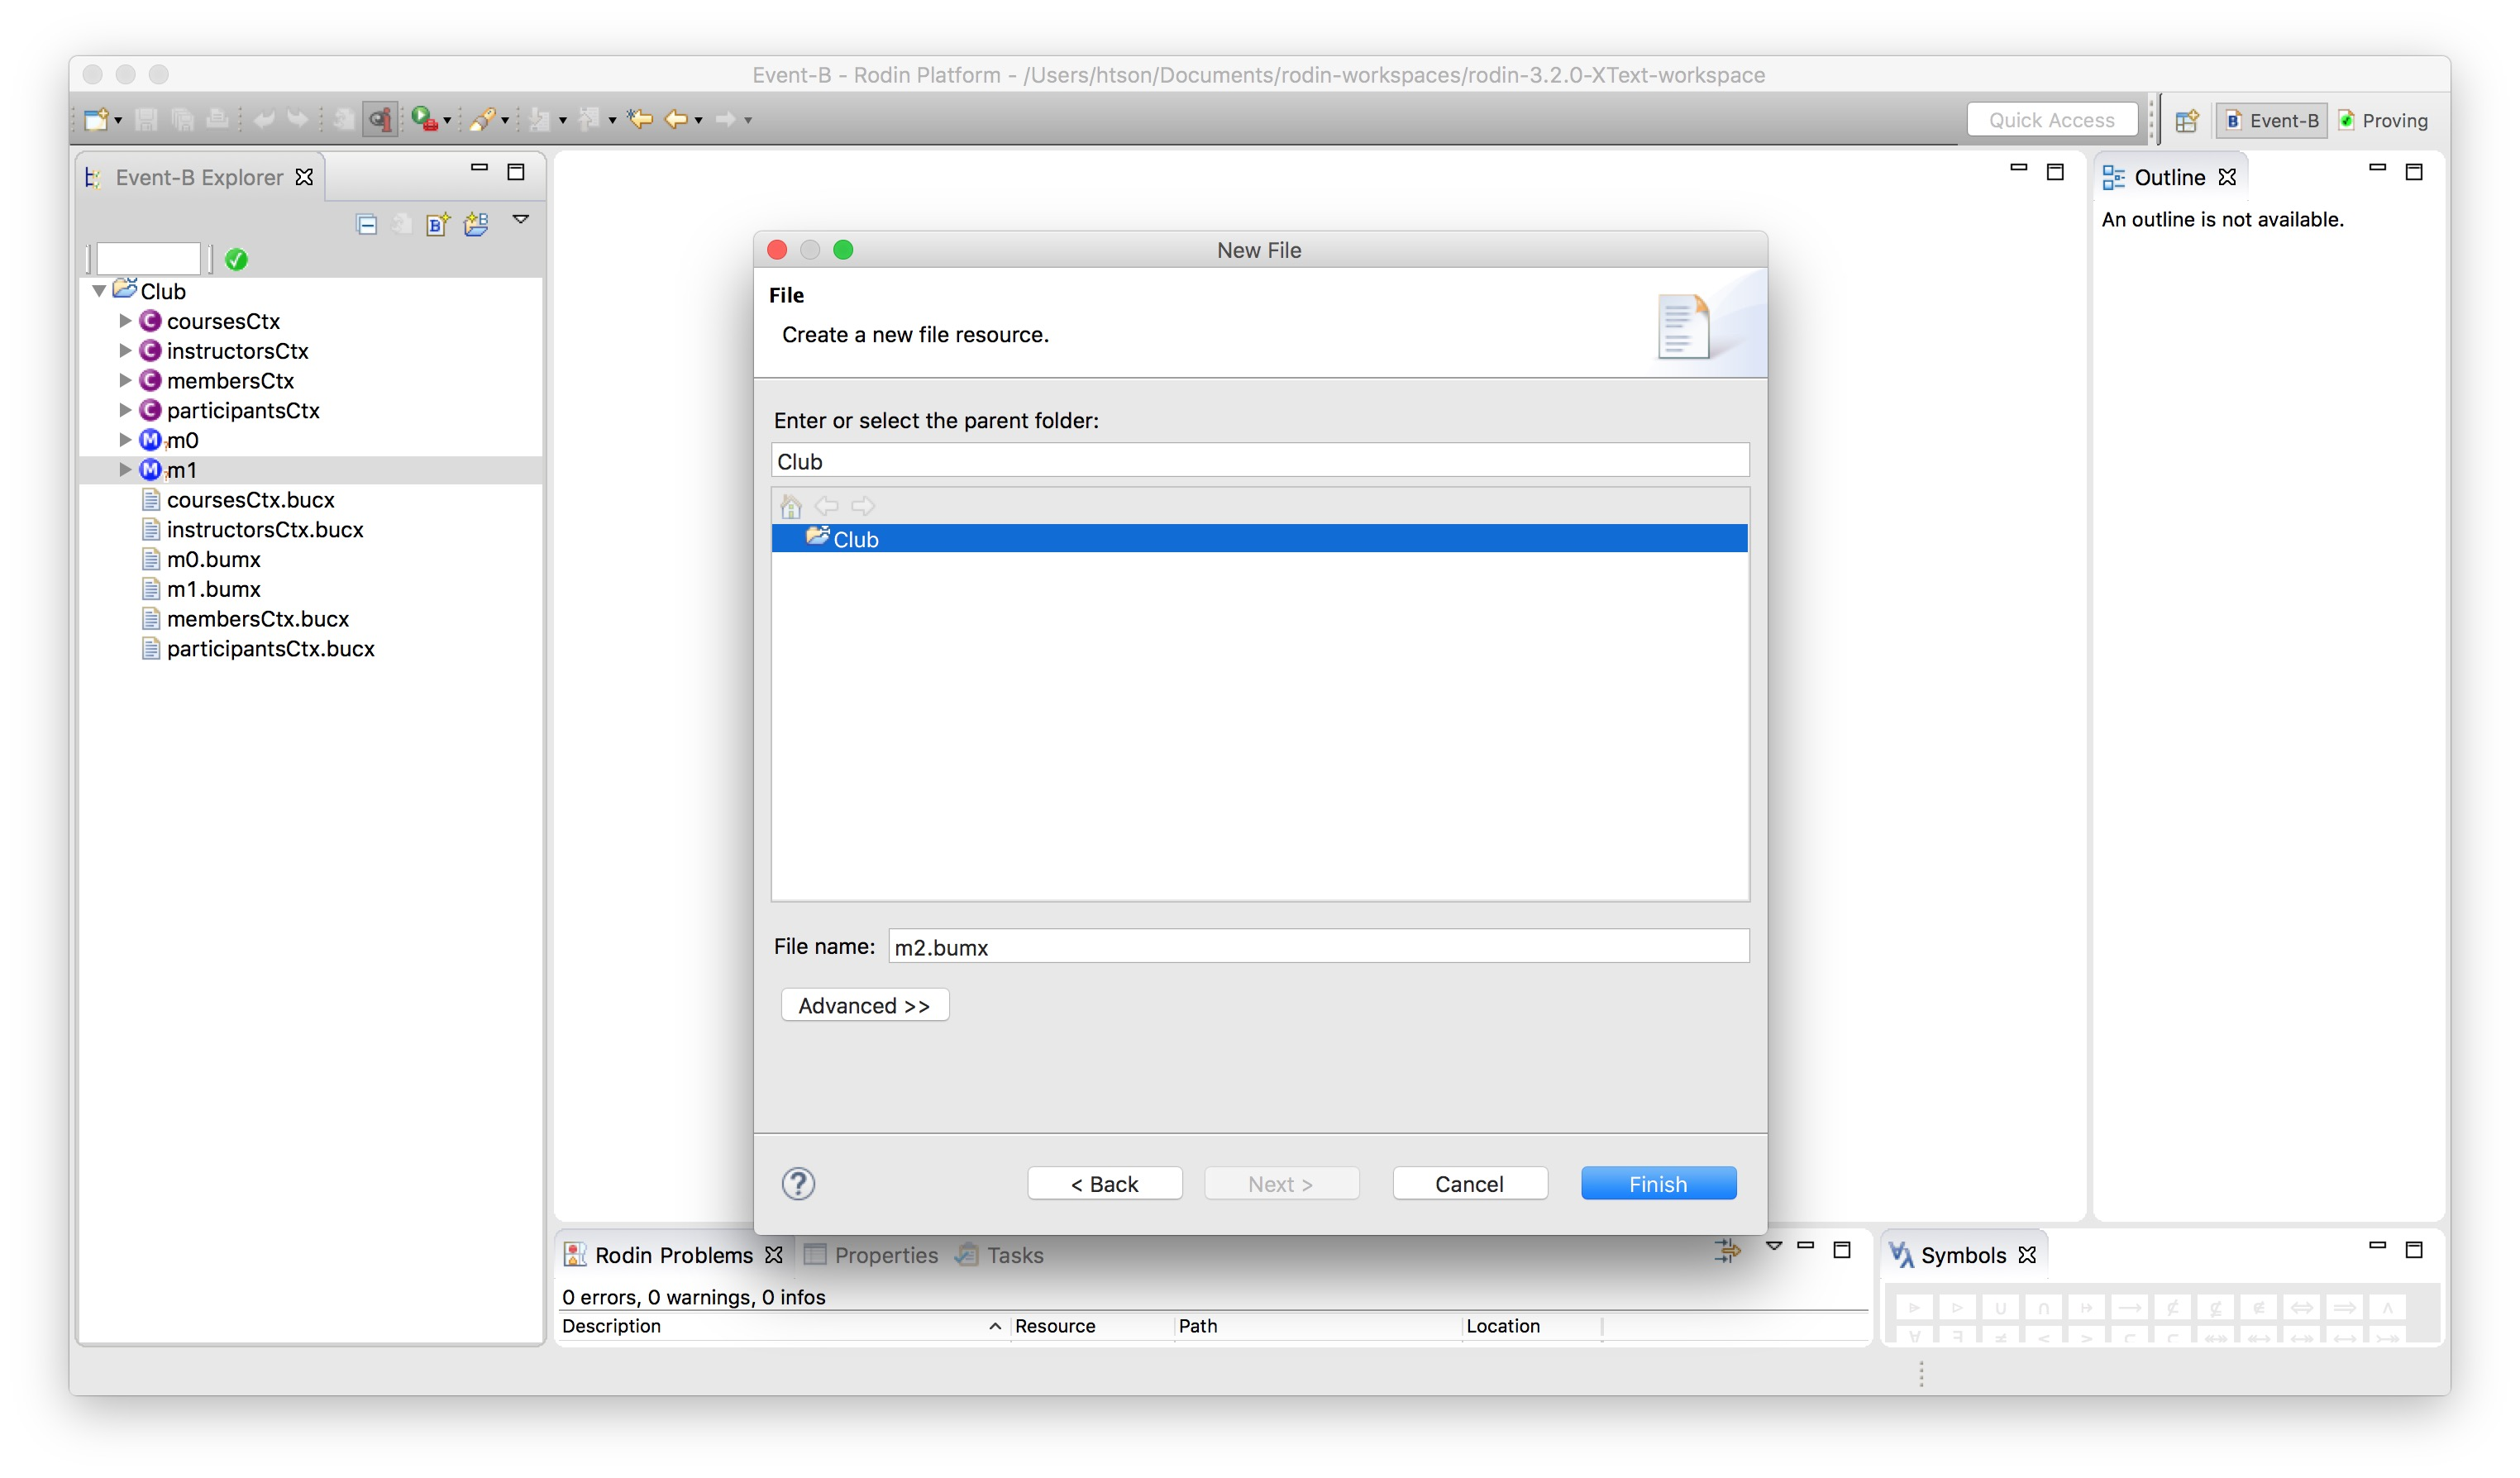
\includegraphics[width=0.9\textwidth]{figures/CreateM2}
    \endif
    \caption{Create m2.bumx}
    \label{fig:CreateM2}
  \end{figure}

\item[Step 2. Set the content of m2.bumx] \textbf{Set the content of ``m2.bumx'' as follows}.
  \begin{center}
    \begin{Bcode}
      \ifdef{PLASTEX}
      \Bmachine{} m2\\
      \Brefines{} m1\\
      \Bsees{} instructorsCtx participantsCtx\\
      \Bvariables{} atnds\\
      \Binvariants\\
      @inv2_1: atnds ∈ CRS ⇸ ℙ(PRTCPT)\\
      @inv2_2: crs = dom(atnds)\\
      @inv2_3: ∀c·c ∈ crs ⇒ prtcpts[\{c\}] = atnds(c)\\
      \Btheorem{} @thm2_1: finite(atnds)\\
      variants @v0: card(atnds)\\
      \Bevents\\
      event INITIALISATION\\
      \Bthen \\
      @act2_1: atnds ≔ ∅\\
      \Bend\\
      event OpenCourse \Brefines{} OpenCourses\\
      \Bany{} c \Bwhere\\
      @grd2_1: c ∉ dom(atnds)\\
      @grd2_2: card(atnds) ≠ m \\
      \Btheorem{} @thm2_2: card(crs) ≠ m\\
      \Bthen\\
      @act2_1: atnds(c) ≔ ∅\\
      \Bwith\\
      @crs': crs' = crs ∪ \{c\}\\
      \Bend\\
      \Bconvergent{} event CloseCourse \\
      \Brefines{} CloseCourses\\
      \Bany{} c \Bwhere\\
      @grd2_1: c ∈ dom(atnds)\\
      \Bthen\\
      @act1_2: atnds ≔\{c\} ⩤ atnds\\
      \Bwith\\
      @cs: cs = \{c\}\\
      \Bend\\
      \Bconvergent{} event Register \\
      \Brefines{} Register\\
      \Bany{} p c \Bwhere\\
      @grd2_1: p ∈ PRTCPT\\
      @grd2_2: p ≠ instrs(c)\\
      @grd2_3: c ∈ dom(atnds)\\
      @grd2_4: p ∉ atnds(c)\\
      \Btheorem{} @thm2_3: atnds(c) = prtcpts[\{c\}]\\
      \Bthen\\
      @act2_1: atnds(c) ≔ atnds(c) ∪ \{p\}\\
      \Bend\\
      \Bend
      \else
      \Bmachine{} m2\\
      \Brefines{} m1\\
      \Bsees{} instructorsCtx participantsCtx\\
      \Bvariables{} atnds\\
      \Binvariants\\
      \Btab @inv2_1: \(atnds \in CRS \pfun \pow(PRTCPT)\)\\
      \Btab @inv2_2: \(crs = \dom(atnds)\)\\
      \Btab @inv2_3: \(\forall c \qdot c \in crs \limp prtcpts[\{c\}] = atnds(c)\)\\
      \Btab \Btheorem{} @thm2_1: \(\finite(atnds)\)\\
      variants @v0: \(\card(atnds)\)\\
      \Bevents\\
      \Btab event INITIALISATION\\
      \Btab \Bthen\\
      \Btab \Btab @act2_1: \(atnds \bcmeq \emptyset\)\\
      \Btab \Bend\\
      \Btab event OpenCourse\\
      \Btab \Brefines{} OpenCourses\\
      \Btab \Bany{} c \Bwhere\\
      \Btab \Btab @grd2_1: \(c \notin \dom(atnds)\)\\
      \Btab \Btab @grd2_2: \(\card(atnds) \neq m\) \\
      \Btab \Btab \Btheorem{} @thm2_2: \(\card(crs) \neq m\)\\
      \Btab \Bthen\\
      \Btab \Btab @act2_1: \(atnds(c) \bcmeq \emptyset\)\\
      \Btab \Bwith\\
      \Btab \Btab @crs': \(crs' = crs \bunion \{c\}\)\\
      \Btab \Bend\\
      \Btab \Bconvergent{} event CloseCourse \\
      \Btab \Brefines{} CloseCourses\\
      \Btab \Bany{} c \Bwhere\\
      \Btab \Btab @grd2_1: \(c \in \dom(atnds)\)\\
      \Btab \Bthen\\
      \Btab \Btab @act1_2: \(atnds \bcmeq \{c\} \domsub atnds\)\\
      \Btab \Bwith\\
      \Btab \Btab @cs: \(cs = \{c\}\)\\
      \Btab \Bend\\
      \Btab  \Bconvergent{} event Register \\
      \Btab \Brefines{} Register\\
      \Btab \Bany{} p c \Bwhere\\
      \Btab \Btab @grd2_1: \(p \in PRTCPT\)\\
      \Btab \Btab @grd2_2: \(p \neq instrs(c)\)\\
      \Btab \Btab @grd2_3: \(c \in \dom(atnds)\)\\
      \Btab \Btab @grd2_4: \(p \notin atnds(c)\)\\
      \Btab \Btab \Btheorem{} @thm2_3: \(atnds(c) = prtcpts[\{c\}]\)\\
      \Btab \Bthen\\
      \Btab \Btab @act2_1: \(atnds(c) \bcmeq atnds(c) ∪ \{p\}\)\\
      \Btab \Bend\\
      \Bend
      \endif
    \end{Bcode}
  \end{center}

\item[Step 3. Auto-format the code] \textbf{Automatically format the content of ``m2.bumx''} by using short-cut (e.g., on Mac OS: Cmd+Shift+F).

\item[Step 4. Save the file] \textbf{Save the file ``m2.bumx''}.
\end{description}
\textbf{Conclusion} By now, the XMachine ``m2.bucx'' and the corresponding Rodin Machine ``m2'' should be visible in the Event-B Explorer (see Figure~\ref{fig:M2}.
  \begin{figure}[!htbp]
    \centering
    \ifdef{PLASTEX}
    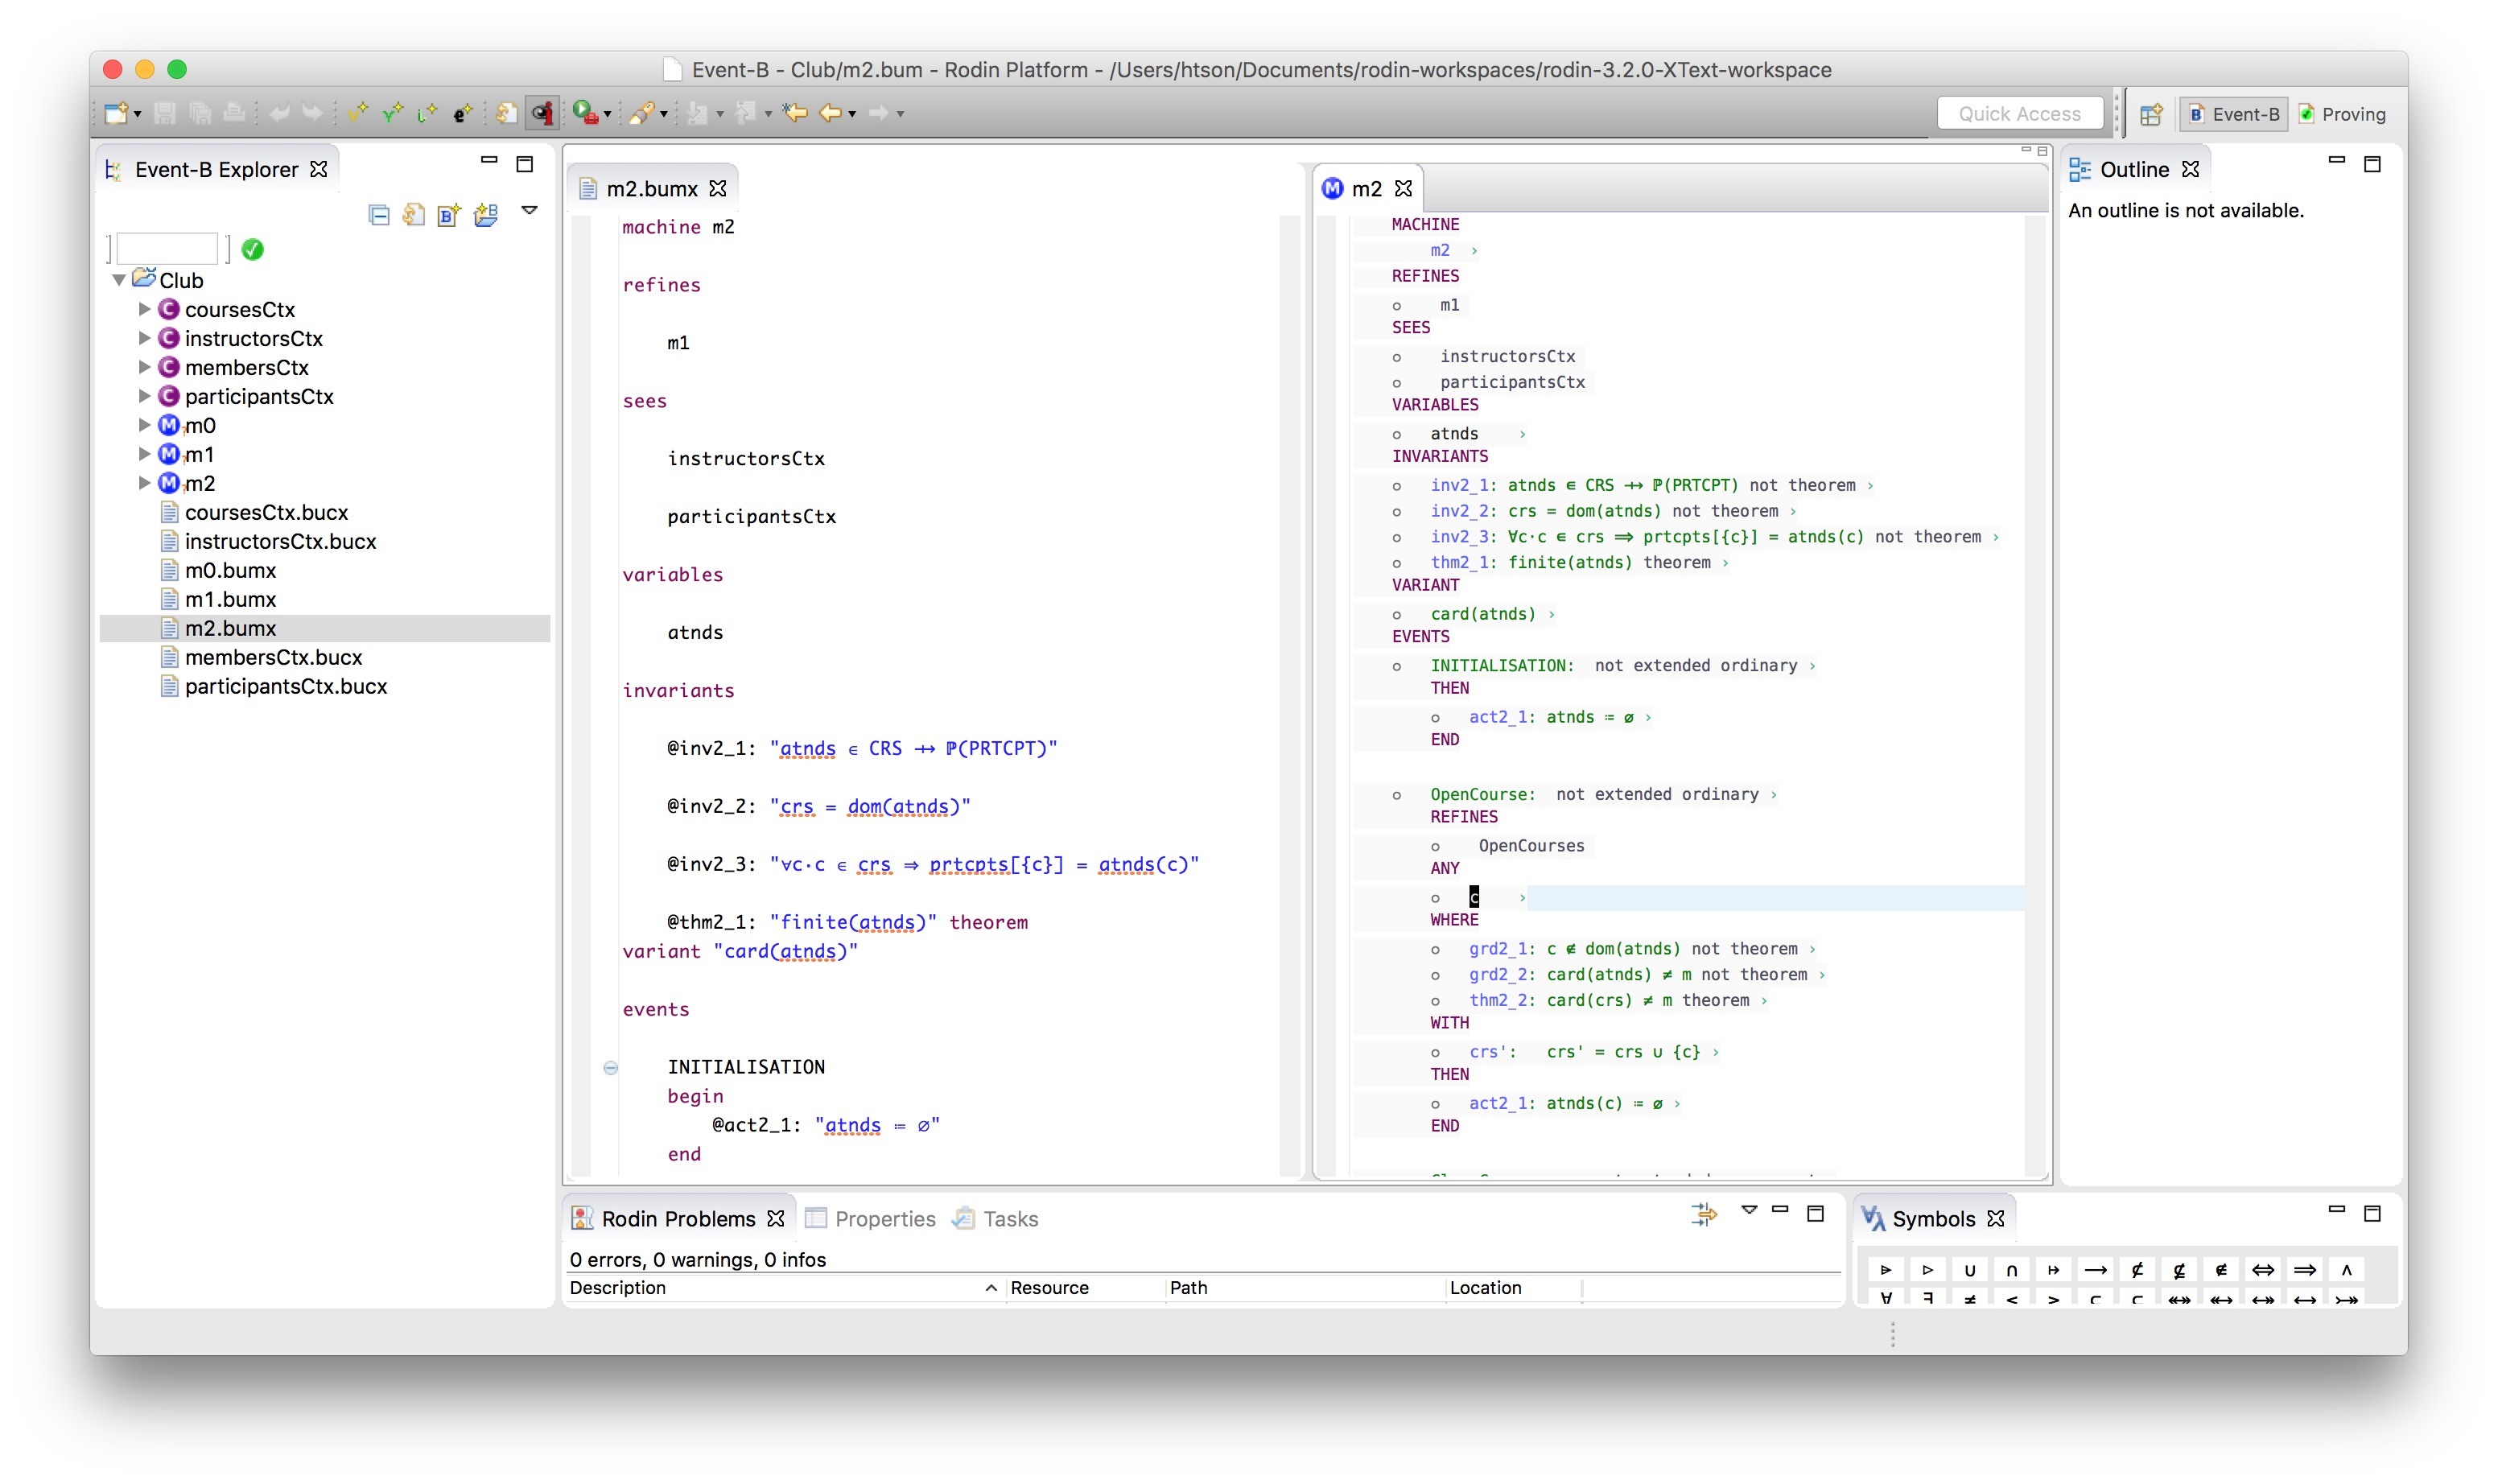
\includegraphics[width=512]{figures/M2}
    \else
    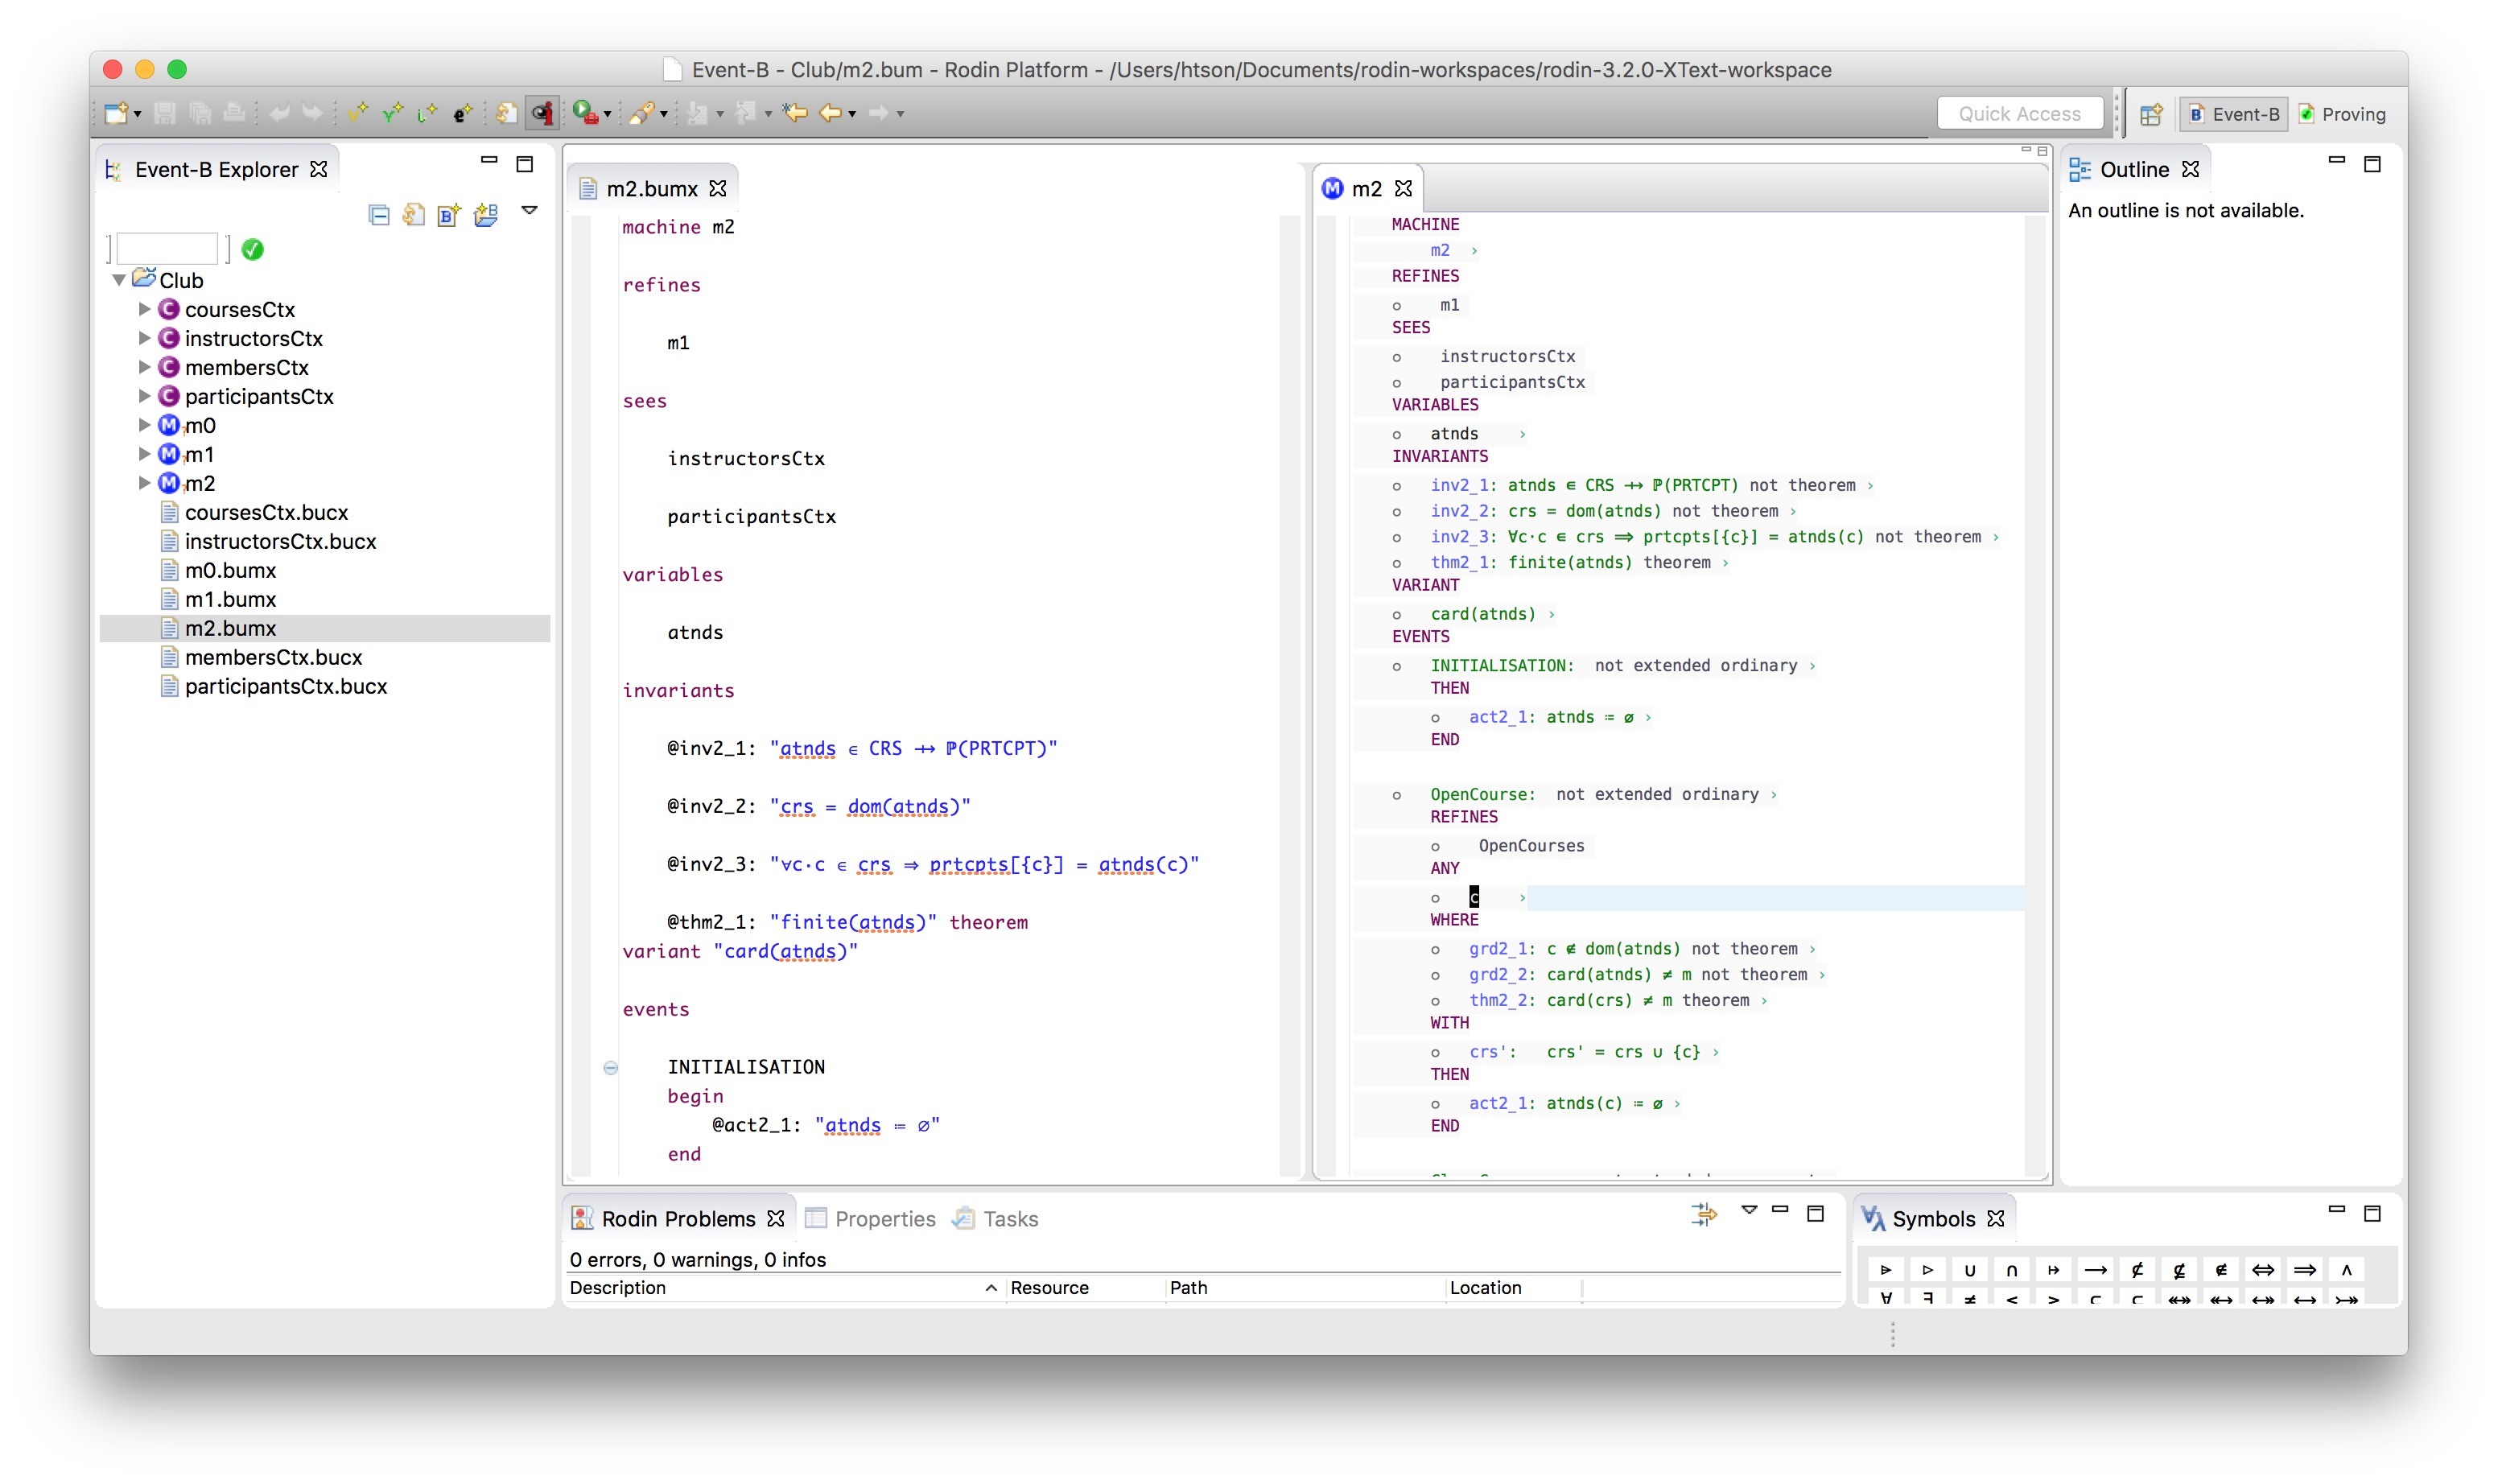
\includegraphics[width=0.9\textwidth]{figures/M2}
    \endif
    \caption{XMachine m2.bumx}
    \label{fig:M2}
  \end{figure}

\subsection{Advanced Tutorial}
\label{sec:advanced-tutorial}

This tutorial provides a step-by-step walk-through working with \emph{machine inclusion} using XEvent-B. Following the same steps as in Section~\ref{sec:basic-tutorial} to create machines and contexts, we can create a machine that can include other machines and can update the included machines variables via \emph{event synchronisation}.

We illustrate the application of machine inclusion using XEvent-B by modelling a small example of ``controlling cars on a bridge'', which is based on Chapter 2 of ``\emph{Modeling in Event-B: System and Software Engineering}'' book.

\subsubsection{Task 1. Create the reusable model}
\textbf{Introduction} The purpose of this task is to create the model that will be reused by other models using machine inclusion.
\begin{description}
\item[Step 1. Create a new Project (Sensor) with XMachine m0\_SNSR.bumx] 

Following the same steps as 
\ifdef{PLASTEX}
in tasks 2 and 4 in Section~\ref{sec:basic-tutorial} for creating project and machines.
\else
in Sections~\ref{CreateProject} and~\ref{CreateMachine} for creating project and machines.
\endif

\item[Step 2. Set the content of m0\_SNSR.bumx] \textbf{Set the content of ``m0\_SNSR.bumx'' as follows}.
\begin{center}
	\begin{Bcode}
		\ifdef{PLASTEX}
		\Bmachine{} m0_SNSR\\
		\Bvariables{} SNSR\\
		\Binvariants\\
                \Btheorem{} @thm0_1: SNSR ∈ BOOL\\
		\Bevents\\
		event INITIALISATION\\
		\Bthen\\
		@act1: SNSR ≔ FALSE\\
		\Bend\\
		event SNSR_on\\
		\Bwhere\\
		@grd1: SNSR = FALSE\\
		\Bthen\\
		@act1: SNSR ≔ TRUE\\
		\Bend\\
	    event SNSR_off\\
	    \Bwhere\\
	    @grd1: SNSR = TRUE\\
	    \Bthen\\
	    @act1: SNSR ≔ FALSE\\
	    \Bend\\
		\Bend
		\else
		\Bmachine{} m0_SNSR\\
		\Bvariables{} SNSR\\
		\Binvariants\\
		\Btab  \Btheorem{} @thm0_1: \(SNSR \in BOOL\)\\
		\Bevents\\
		\Btab event INITIALISATION\\
		\Btab \Bthen\\
		\Btab \Btab @act1: \(SNSR \bcmeq FALSE\)\\
		\Btab \Bend\\
		\Btab event SNSR_on\\
		\Btab \Bwhere\\
		\Btab \Btab @grd1: \(SNSR = FALSE\)\\
		\Btab \Bthen\\
		\Btab \Btab @act1: \(SNSR \bcmeq TRUE\)\\
		\Btab \Bend\\
		\Btab event SNSR_off\\
		\Btab \Bwhere\\
		\Btab \Btab @grd1: \(SNSR = TRUE\)\\
		\Btab \Bthen\\
		\Btab \Btab @act1: \(SNSR \bcmeq FALSE\)\\
		\Btab \Bend\\
		\Bend
		\endif
	\end{Bcode}
\end{center}

\item[Step 3. Auto-format and Save the file ``m0\_SNSR.bumx''] 
\end{description}

\textbf{Conclusion} By now, the XMachine ``m0\_SNSR.bumx'' and the corresponding Rodin Machine ``m0\_SNSR'' should be visible in the Event-B Explorer.

\subsubsection{Task 2. Model the abstract level of cars on a bridge}
\textbf{Introduction} The purpose of this task is to create the abstract model of the ``cars on a bridge'' example. At this level, we have not applied machine inclusion, but it is possible to apply machine inclusion right from the abstract level. 
\begin{description}
	\item[Step 1. Create the Context Car\_c0\_limit.bucx in a new project Car] 
	Following the same steps as 
	\ifdef{PLASTEX}
	in task 3 of Section~\ref{sec:basic-tutorial} for creating a simple context.  
	\else
	in Section~\ref{Sec:SimpleContext} for creating a simple context.
	\endif
	\textbf{Set the content of ``Car\_c0\_limit.bucx'' as follows and save the file}.
	  
	  \begin{center}
		\begin{Bcode}
			\ifdef{PLASTEX}
			\Bcontext{} Car\_c0_limit\\
			\Bconstants{} D\\
			\Baxioms\\
			@axm1: D ∈ ℕ1\\
			\Bend
			\else
			\Bcontext{} Car_c0_limit\\
			\Bconstants{} D\\
			\Baxioms\\
			\Btab @axm1: \(D \in \nat1\)\\
			\Bend
			\endif
		\end{Bcode}
	\end{center}
	\item[Step 2. Create the Machine Car\_m0\_cars.bumx]\textbf{Set the content of ``Car\_m0\_cars.bumx'' as follows and save the file}.

	\begin{center}
		\begin{Bcode}
			\ifdef{PLASTEX}
			\Bmachine{} Car\_m0_cars\\
			\Bsees{} Car\_c0_limit\\
			\Bvariables{} A B C\\
			\Binvariants\\
			@inv0_1: A ∈ ℕ\\
			@inv0_2: B ∈ ℕ\\
			@inv0_3: C ∈ ℕ\\
			@inv0_4: A = 0 ∨ C = 0\\
			@inv0_5: A + B + C ≤ D\\
                        \Btheorem{} @thm0_1: B ≤ D\\
			\Bevents\\
			event INITIALISATION\\
			\Bthen\\
			@act1: A ≔ 0\\
			@act2: B ≔ 0\\
			@act3: C ≔ 0\\
			\Bend\\
			event ML_out\\
			\Bwhere\\
			@grd1: C = 0\\
			@grd2: A + B ≠ D\\
			\Bthen\\
			@act1: A ≔ A + 1\\
			\Bend\\
			event ML_in\\
			\Bwhere\\
			@grd1: C ≠ 0\\
			\Bthen\\
			@act1: C ≔ C − 1\\
			\Bend\\
			event IL_in\\
			\Bwhere\\
			@grd1: A ≠ 0\\
			\Bthen\\
			@act1: A ≔ A − 1\\
			@act2: B ≔ B + 1\\
			\Bend\\
			event IL_out\\
			\Bwhere\\
			@grd1: B ≠ 0\\
			@grd2: A = 0\\
			\Bthen\\
			@act1: B ≔ B − 1\\
			@act2: C ≔ C + 1\\
			\Bend\\
			\Bend
			\else
			\Bmachine{} Car\_m0_cars\\
			\Bsees{} Car\_c0_limit\\
			\Bvariables{} A B C\\
			\Binvariants\\
			\Btab @inv0_1: \(A \in \nat\)\\
			\Btab @inv0_2: \(B \in \nat\)\\
			\Btab @inv0_3: \(C \in \nat\)\\
			\Btab @inv0_4: \(A = 0 \vee C = 0\)\\
			\Btab @inv0_5: \(A + B + C \leq D\)\\
			\Btab  \Btheorem{} @thm0_1: \(B \leq D\)\\
			\Bevents\\
			\Btab event INITIALISATION\\
			\Btab \Bthen\\
			\Btab \Btab @act1: \(A \bcmeq 0\)\\
			\Btab \Btab @act2: \(B \bcmeq 0\)\\
			\Btab \Btab @act3: \(C \bcmeq 0\)\\
			\Btab \Bend\\
			\Btab event ML_out\\
			\Btab \Bwhere\\
			\Btab \Btab @grd1: \(C = 0\)\\
			\Btab \Btab @grd2: \(A + B \neq D\)\\
			\Btab \Bthen\\
			\Btab \Btab @act1: \(A \bcmeq A + 1\)\\
			\Btab \Bend\\
			\Btab event ML_in\\
			\Btab \Bwhere\\
			\Btab \Btab @grd1: \(C \neq 0\)\\
			\Btab \Bthen\\
			\Btab \Btab @act1: \(C \bcmeq C - 1\)\\
			\Btab \Bend\\
			\Btab event IL_in\\
			\Btab \Bwhere\\
			\Btab \Btab @grd1: \(A \neq 0\)\\
			\Btab \Bthen\\
			\Btab \Btab @act1: \(A \bcmeq A - 1\)\\
			\Btab \Btab @act2: \(B \bcmeq B + 1\)\\
			\Btab \Bend\\
			\Btab event IL_out\\
			\Btab \Bwhere\\
			\Btab \Btab @grd1: \(B \neq 0\)\\
			\Btab \Btab @grd2: \(A = 0\)\\
			\Btab \Bthen\\
			\Btab \Btab @act1: \(B \bcmeq B - 1\)\\
			\Btab \Btab @act2: \(C \bcmeq C + 1\)\\
			\Btab \Bend\\
			\Bend
			\endif
		\end{Bcode}
	\end{center}
	
\end{description}
\textbf{Conclusion} Saving the XContext and XMachine files will generate the corresponding Rodin files. In the ``Car'' you have the context ``Car\_c0\_limit'' and the machine ``Car\_m0\_cars''. Ideally the reusable models should be in a different project, that is why we added the reusable model in a different project ``Sensor''.

\subsubsection{Task 3. Model an XMachine using machine inclusion}
\textbf{Introduction} In this task we define the XMachine ``Car\_m1\_SNSR.bumx'' which is a refinement of the machine ``Car\_m0\_cars'' and includes two instances of ``m0\_SNSR''. The keywords in red  are \textbf{not} part of the standard Event-B syntax, they correspond to machine inclusion and event synchronisation. 

\begin{description}
	\item[Step 1. Create the file ``Car\_m1\_SNSR.bumx''] \textbf{Set its contents as follows.}
	
		\begin{center}
		\begin{Bcode}
			\ifdef{PLASTEX}
			\Bmachine{} Car_m1_SNSR\\
			\textcolor{red}{\textbf{includes}} Sensor.m0_SNSR \textcolor{red}{\textbf{as}} IL_out ML_out\\
			\Brefines{} Car_m0_cars\\
			\Bsees{} Car_c0_limit\\
			\Bvariables{} A B C\\
			\Binvariants\\
			@inv1_1: IL_out_SNSR = TRUE ⇒ B ≠ 0\\
			\Bevents\\
			event INITIALISATION extends INITIALISATION\\
			\textcolor{red}{\textbf{synchronises}} IL_out.INITIALISATION\\
			\textcolor{red}{\textbf{synchronises}} ML_out.INITIALISATION\\
			\Bend\\
			event ML_out extends ML_out\\
			\textcolor{red}{\textbf{synchronises}} ML_out.SNSR_off\\
			\Bend\\
			event ML_in extends ML_in\\
			\Bend\\
			event IL_in extends IL_in\\
			\Bwhere\\
			\Btheorem{} @inv0_2−copy: B ∈ ℕ \\
			\Bend\\
			event IL_out \Brefines{} IL_out\\
			\textcolor{red}{\textbf{synchronises}} IL_out.SNSR_off\\
			\Bwhere\\
			@grd2: A = 0\\
			\Bthen\\
			@act1: B ≔ B − 1\\
			@act2: C ≔ C + 1\\
			\Bend\\
			event ML_out_ARR\\
			\textcolor{red}{\textbf{synchronises}} ML_out.SNSR_on\\
			\Bend\\
			event IL_out_ARR\\
			\textcolor{red}{\textbf{synchronises}} IL_out.SNSR_on\\
			\Bwhere\\
			@grd2: B ≠ 0\\
			\Bend\\
			\Bend
			\else
			\Bmachine{} Car_m1_SNSR\\
			\textcolor{red}{includes} Sensor.m0_SNSR \textcolor{red}{as} IL_out ML_out\\
			\Brefines{} Car_m0_cars\\
			\Bsees{} Car_c0_limit\\
			\Bvariables{} A B C\\
			\Binvariants\\
			\Btab @inv1_1: \(IL\_out\_SNSR = TRUE \Rightarrow B \neq 0\)\\
			\Bevents\\
			\Btab event INITIALISATION extends INITIALISATION\\
			\Btab \textcolor{red}{synchronises} IL_out.INITIALISATION\\
            \Btab \textcolor{red}{synchronises} ML_out.INITIALISATION\\
			\Btab \Bend\\
			\Btab event ML_out extends ML_out\\
			\Btab \textcolor{red}{synchronises} ML_out.SNSR_off\\
			\Btab \Bend\\
			\Btab event ML_in extends ML_in\\
			\Btab \Bend\\
			\Btab event IL_in extends IL_in\\
			\Btab \Bwhere\\
			\Btab \Btab @inv0_2−copy: "\(B \in \nat\)" \Btheorem\\
			\Btab \Bend\\
			\Btab IL_out \Brefines{} IL_out\\
			\Btab \textcolor{red}{synchronises} IL_out.SNSR_off\\
			\Btab \Bwhere\\
			\Btab \Btab @grd2: \(A = 0\)\\
			\Btab \Bthen\\
			\Btab \Btab @act1: \(B \bcmeq B - 1\)\\
			\Btab \Btab @act2: \(C \bcmeq C + 1\)\\
			\Btab \Bend\\
			\Btab event ML_out_ARR\\
			\Btab \textcolor{red}{synchronises} ML_out.SNSR_on\\
			\Btab \Bend\\
			\Btab event IL_out_ARR\\
			\Btab \textcolor{red}{synchronises} IL_out.SNSR_on\\
			\Btab \Bwhere\\
			\Btab \Btab @grd2: \(B \neq 0\)\\
			\Btab \Bend\\
			\Bend
			\endif
		\end{Bcode}
	\end{center}
	\item[Step 2. Auto-format the file ``Car\_m1\_SNSR.bumx'' and Save it.]
\end{description}
\textbf{Conclusion} After saving the file a standard Event-B machine ``Car\_m1\_SNSR''will be generated. The generated machine (Figure~\ref{fig:FlattenedMachine}) is flattened to include the variables and invariants  of the included machine ``m0\_SNSR'' which are renamed according to the chosen prefixes. In addition to the guards and actions of the synchronised events. The project name must be specified when including a machine (e.g., Sensor.m0\_SNSR), and the project (Sensor) of the included machines must be opened in the same workspace. You can also use content assist to see all available machines in the workspace.

When synchronising an event you can add the prefix of the required machine followed by the synchronised event name (e.g., IL\_out.SNSR\_on where ``IL\_out'' is one of the included machine prefixes and ``SNSR\_on'' is the synchronised event). It is also possible to include more than one machine and synchronise with more than one event. Notice the order of the generated elements in the flattened machine is the included elements from last to first then the source machine elements.

\begin{figure}[!htbp]
	\centering
	\ifdef{PLASTEX}
	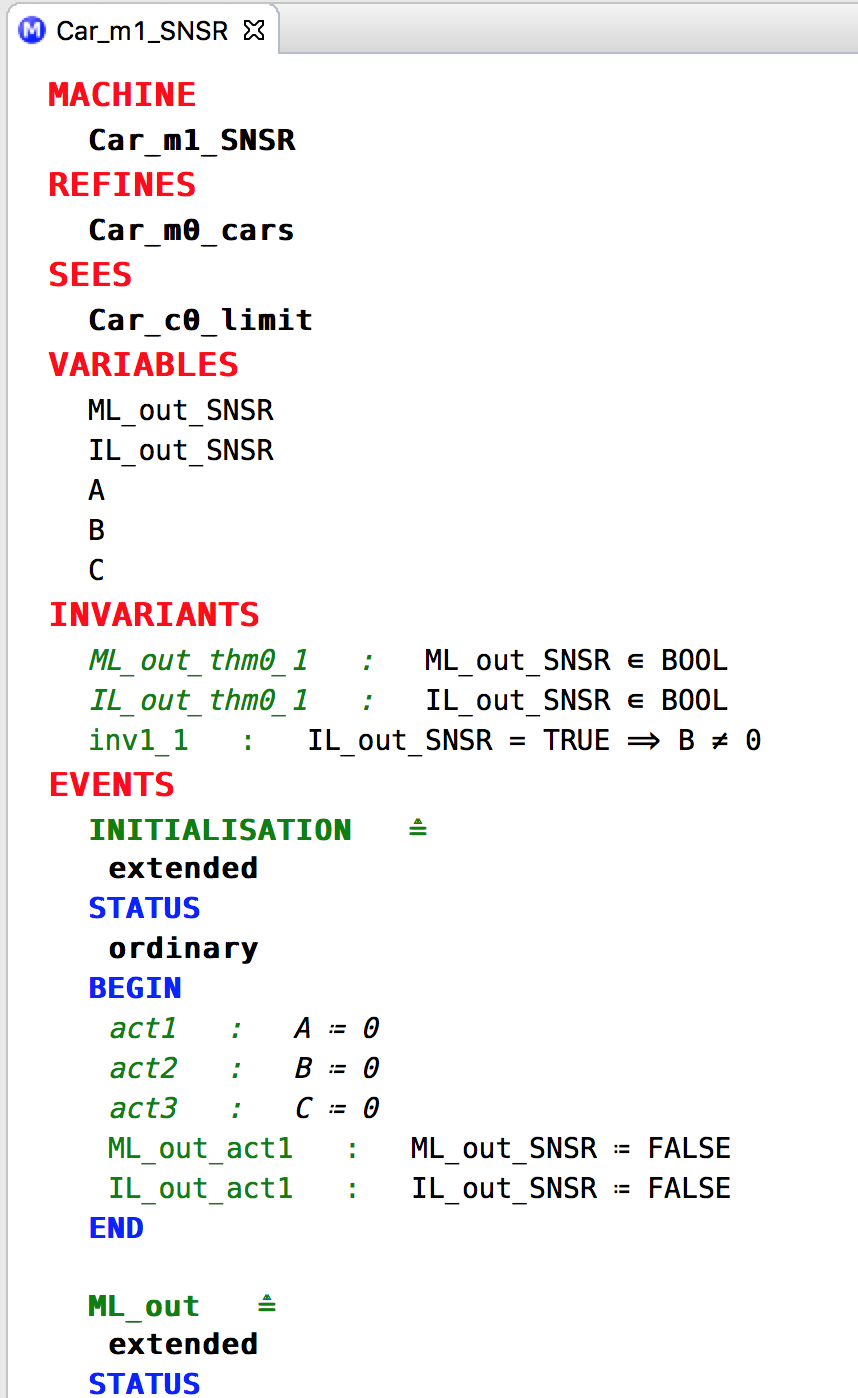
\includegraphics[width=512]{figures/Flattened_var_m1_snsr}
	\else
	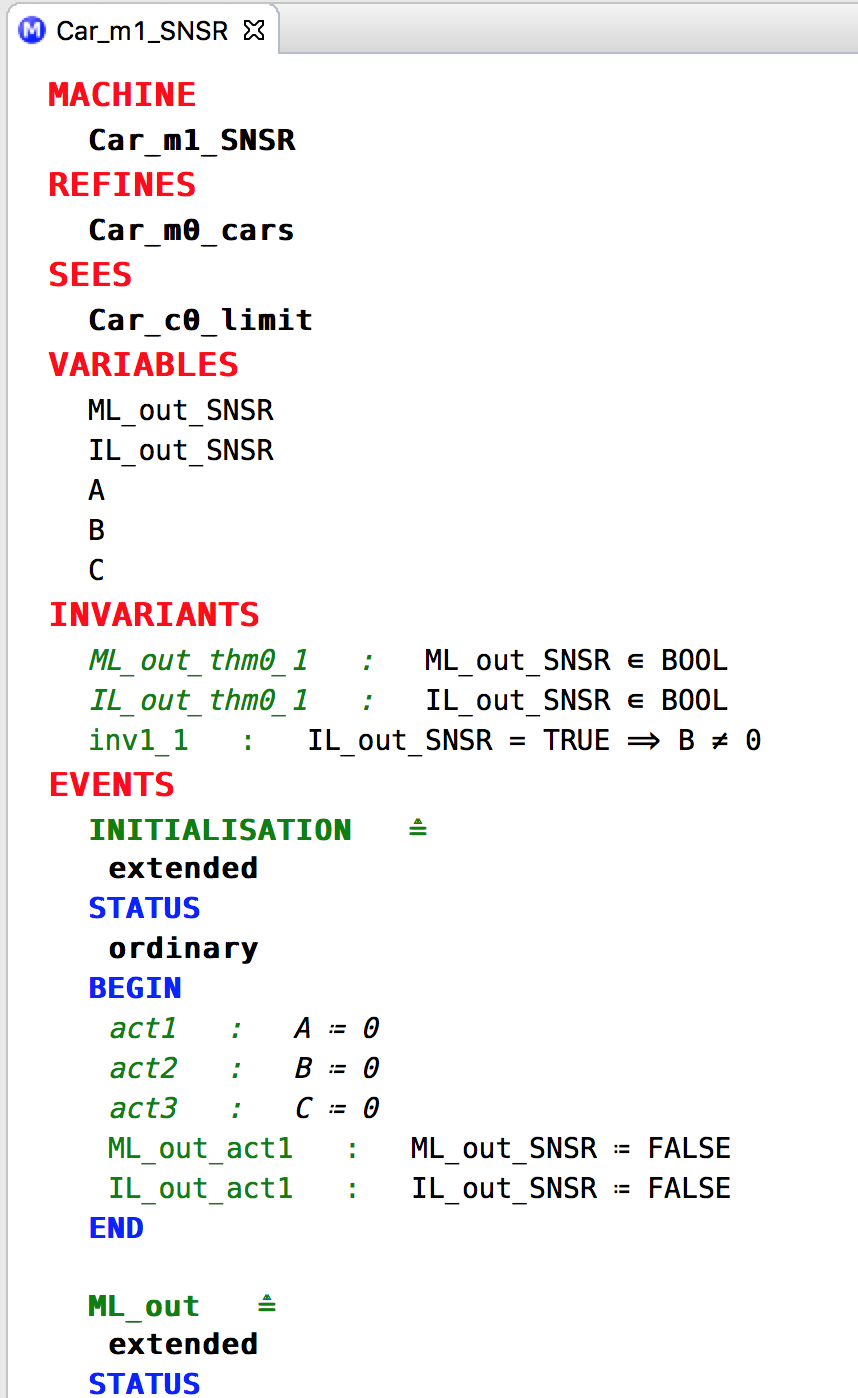
\includegraphics[width=0.9\textwidth]{figures/Flattened_var_m1_snsr}
	\endif
	\caption{Flattened Machine ``Car\_m1\_SNSR''}
	\label{fig:FlattenedMachine}
\end{figure}

% probably here add a figure of the flattened machine to show how variables, inv, gurads are copied and renamed

%%% Local Variables:
%%% mode: latex
%%% TeX-master: "user_manual"
%%% End:
